%\documentclass[fleqn,reqno,a4paper,parskip=half]{scrartcl}
\documentclass[fleqn,reqno,a4paper,parskip=half]{scrbook}
%\usepackage{showkeys}      % zeigt label-Bezeichner an

%%%%%%%%%%%%%%%%   Pakete   %%%%%%%%%%%%%%%%%%

\usepackage{charter} %Charter fuer englische Texte
%\linespread{1.05} % Durchschuss für Charter leicht erhöhen

%\usepackage[mathletters]{ucs} %direkt griechisches im Mathe modus
%\usepackage[utf8]{inputenc}
\usepackage[utf8]{inputenc}
%\usepackage[utf8x]{inputenc}
%\usepackage[T1]{fontenc}
%\usepackage{times}

% utf8x is incompatible with biblatex, the following trick is a remedy
% source: https://tex.stackexchange.com/a/213177
\input{binhex}
\makeatletter
\def\uc@dclc#1#2#3{%
  \ifnum\pdfstrcmp{#2}{mathletters}=\z@
    \begingroup\edef\x{\endgroup
      \noexpand\DeclareUnicodeCharacter{\hex{#1}}}\x{#3}%
  \fi
}
\input{uni-3.def}
\def\uc@dclc#1#2#3{%
  \ifnum\pdfstrcmp{#2}{default}=\z@
    \begingroup\edef\x{\endgroup
      \noexpand\DeclareUnicodeCharacter{\hex{#1}}}\x{#3}%
  \fi
}
\input{uni-34.def}
\makeatother






%TODO_Lorin: besser?
   %\usepackage{uniinput}       % für Unicode-Zeichen, wird momentan nicht verwendet, deshalb auskommentiert by Benni


%\usepackage[ngerman]{babel}
%\usepackage{ngerman}
\usepackage[tbtags,sumlimits,intlimits,namelimits]{amsmath}

\usepackage{amsfonts}
\usepackage{amssymb}
\usepackage{bbm}
\usepackage{ulem}
\usepackage{tikz}
\usepackage{pgf}
\usepackage{ifpdf}
\usepackage{color}
\usepackage{esint}
\usepackage{framed}
\usepackage{wasysym}  % \ocircle
%\usepackage{calc}   % \begin{tabular}[b]{|p{\textwidth-2\tabcolsep}|}

%\usepackage[colorlinks=true,linkcolor=black,citecolor=black,urlcolor=black]{hyperref}  % print
\usepackage[colorlinks=true,linkcolor=blue,citecolor=blue]{hyperref}    % web
\usepackage[top=2.3cm, bottom=3.45cm, left=2.3cm, right=2.3cm]{geometry}
%\numberwithin{equation}{section}
\usepackage{chngcntr}
\counterwithin*{section}{part}
%\graphicspath{{images/png/}{images/}}        % Pfad, in dem sich Grafikdateien befinden
%\usepackage{subfigure}          % Unterbilder, deprecated
%\usepackage(subfig}

\usepackage[all]{hypcap}
%\usepackage{cite}           % Literatur
\usepackage{graphicx}       % Bilder in Tabellen
\usepackage{float}          % eigene Float-Umgebungen, H-Option, um Bilder an der aktuellen Stelle anzuzeigen
\usepackage{caption}
\usepackage{subcaption,array}
%\usepackage{array}

\restylefloat{figure}       % Bilder an der Stelle, wo sie eingebunden werden
\usepackage{multirow}
\usepackage{listings}       % Darstellung von Source-Code
\usepackage{framed}         % Rahmen um Text
\usepackage{arydshln}       % gestrichelte Linie in Tabelle mit \hdashline
\usepackage{longtable}     % Tabellen mit automatischen Seitenumbruch
\usepackage{layouts}        % textwidth in cm: \printinunitsof{cm}\prntlen{\textwidth}
 % \cref verbessert
\usepackage[
  % capitalize names automatically
  capitalise,
  % mark all of "Lemma 1" as a link, not only "1"
  nameinlink,
  % pass language used in document to enable cleveref in otherlanguage env
  ngerman,english,
]{cleveref}
%\usepackage{ziffer}       % Komma in Dezimalzahlen
\usepackage{url}          % Links
%% end old
\definecolor{darkblue}{rgb}{0,0,.5}
\definecolor{black}{rgb}{0,0,0}

\usepackage[framemethod=TikZ]{mdframed}       % Rahmen um Text und Gleichungen


%\usepackage{arydshln}      % gestrichelte Linie in Tabelle mit \hdashline
\usepackage{dirtytalk}          % \say{...} erzeugt (deutsche) Anführungszeichen

\usepackage{tipa}
\usepackage{transparent}    % needed for inkscape generated pdf_tex files
\usepackage{multicol}       % multiple columns
\usepackage{moreverb}       % verbatimwrite
\usepackage{verbatimbox}    % \begin{verbbox}
\usepackage{booktabs}
\usepackage{morefloats}     % Increase the number of simultaneous LaTeX floats
\usepackage{enumitem}       % more control oover itemize
%\usepackage{algorithm2e}
%\usepackage{algorithmic}
%\usepackage{algpseudocode}

\newsavebox\lstbox
\mdfdefinestyle{MyFrame}{%
    innertopmargin=0pt,
    innerbottommargin=10pt,
    innerrightmargin=20pt,
    innerleftmargin=20pt}

\definecolor{darkgreen}{HTML}{009900}
    
% settings for algorithm
\lstset{literate=%
    {Ö}{{\"O}}1
    {Ä}{{\"A}}1
    {Ü}{{\"U}}1
    {ß}{{\ss}}1
    {ü}{{\"u}}1
    {ä}{{\"a}}1
    {ö}{{\"o}}1
    {⇐}{{$\leftarrow$}}1
    {>=}{{$\geq$}}1
    {~}{{\textasciitilde}}1,  
  language=C++,
  numbers=none,
  numberstyle=\tiny,
  xleftmargin=2.0ex, 
  %basicstyle=\small, %  print  whole  listing  small
  basicstyle=\small\ttfamily,
  morekeywords={elif,do,end,then,proc,local,Eingabe,Ausgabe,alignof,loop,each},
  deletekeywords={new},
  columns=flexible,   % alignment
  tabsize=2,    % size of tabs
  keepspaces,
  gobble=2,    % remove 2 characters at begin of each line
  mathescape    % wandle $$ in latex um
}

% Versuche stärker, Abbildungen dort einzubinden, wo sie definiert wurden
\renewcommand{\topfraction}{.85}      % Anteil, den floats auf einer Seite von oben her einnehmen dürfen
\renewcommand{\bottomfraction}{.7}    % Anteil, den floats auf einer Seite von unten her einnehmen dürfen
\renewcommand{\textfraction}{.15}       % Anteil der Seite, der mind. für Text zur Verfügung steht
\renewcommand{\floatpagefraction}{.66}  % Anteil der Seite, der belegt sein muss, bevor eine weitere Seite angelegt wird
\setcounter{topnumber}{9}               % maximale Anzahl floats, die im oberen Bereich der Seite sein dürfen
\setcounter{bottomnumber}{9}            % maximale Anzahl floats, die im unteren Bereich der Seite sein dürfen
    

\usepackage{charter} %Charter fuer englische Texte
%\linespread{1.05} % Durchschuss für Charter leicht erhöhen

\usepackage[utf8]{inputenc}
\usepackage{pmboxdraw}

% utf8x is incompatible with biblatex, the following trick is a remedy
% source: https://tex.stackexchange.com/a/213177
\input{binhex}
\makeatletter
\def\uc@dclc#1#2#3{%
  \ifnum\pdfstrcmp{#2}{mathletters}=\z@
    \begingroup\edef\x{\endgroup
      \noexpand\DeclareUnicodeCharacter{\hex{#1}}}\x{#3}%
  \fi
}
\input{uni-3.def}
\def\uc@dclc#1#2#3{%
  \ifnum\pdfstrcmp{#2}{default}=\z@
    \begingroup\edef\x{\endgroup
      \noexpand\DeclareUnicodeCharacter{\hex{#1}}}\x{#3}%
  \fi
}
\input{uni-34.def}
\makeatother

\usepackage[tbtags,sumlimits,intlimits,namelimits]{amsmath}

\usepackage{amsfonts}
\usepackage{amssymb}
\usepackage{bbm}
\usepackage{ulem}
\usepackage{tikz}
\usepackage{pgf}
\usepackage{ifpdf}
\usepackage{color}
\usepackage{esint}
\usepackage{framed}
\usepackage{wasysym}  % \ocircle
\usepackage{makecell}  % \makecell{...\\...} to break in table cell
\usepackage{textcomp}
\usepackage{fancyvrb}  % improved verbatim 


%\usepackage[colorlinks=true,linkcolor=black,citecolor=black,urlcolor=black]{hyperref}  % print
%\usepackage[colorlinks=true,linkcolor=blue,citecolor=blue,pdfpagelabels,plainpages=false]{hyperref}    % web
%\usepackage{hyperref}    % plain
\usepackage[top=2.3cm, bottom=3.45cm, left=2.3cm, right=2.3cm]{geometry}
%\numberwithin{equation}{section}
\usepackage{chngcntr}
\counterwithin*{section}{part}
%\graphicspath{{images/png/}{images/}}        % Pfad, in dem sich Grafikdateien befinden
%\usepackage{subfigure}          % Unterbilder, deprecated
%\usepackage(subfig}

%\usepackage{cite}           % Literatur
\usepackage{graphicx}       % Bilder in Tabellen
\usepackage{float}          % eigene Float-Umgebungen, H-Option, um Bilder an der aktuellen Stelle anzuzeigen
\usepackage{caption}
\usepackage{subcaption,array}
%\usepackage{array}

\restylefloat{figure}       % Bilder an der Stelle, wo sie eingebunden werden
\usepackage{multirow}
\usepackage{listings}       % Darstellung von Source-Code
\usepackage{framed}         % Rahmen um Text
\usepackage{arydshln}       % gestrichelte Linie in Tabelle mit \hdashline
\usepackage{longtable}     % Tabellen mit automatischen Seitenumbruch
\usepackage{layouts}        % textwidth in cm: \printinunitsof{cm}\prntlen{\textwidth}
 
%\usepackage{ziffer}       % Komma in Dezimalzahlen
\usepackage{url}          % Links
%% end old
\definecolor{darkblue}{rgb}{0,0,.5}
\definecolor{black}{rgb}{0,0,0}

\usepackage[framemethod=TikZ]{mdframed}       % Rahmen um Text und Gleichungen


%\usepackage{arydshln}      % gestrichelte Linie in Tabelle mit \hdashline
\usepackage{dirtytalk}          % \say{...} erzeugt (deutsche) Anführungszeichen

\usepackage{tipa}
\usepackage{transparent}    % needed for inkscape generated pdf_tex files
\usepackage{multicol}       % multiple columns
\usepackage{moreverb}       % verbatimwrite
\usepackage{verbatimbox}    % \begin{verbbox}
\usepackage{booktabs}
\usepackage{morefloats}     % Increase the number of simultaneous LaTeX floats
\usepackage{enumitem}       % more control oover itemize
%\usepackage{algorithm2e}
%\usepackage{algorithmic}
%\usepackage{algpseudocode}

\newsavebox\lstbox
\mdfdefinestyle{MyFrame}{%
    innertopmargin=0pt,
    innerbottommargin=10pt,
    innerrightmargin=20pt,
    innerleftmargin=20pt}

\definecolor{darkgreen}{HTML}{009900}
    
% settings for algorithm
\lstset{literate=%
    {Ö}{{\"O}}1
    {Ä}{{\"A}}1
    {Ü}{{\"U}}1
    {ß}{{\ss}}1
    {ü}{{\"u}}1
    {ä}{{\"a}}1
    {ö}{{\"o}}1
    {⇐}{{$\leftarrow$}}1
    {>=}{{$\geq$}}1
    {~}{{\textasciitilde}}1
    {`}{\textquotedbl}1,  
  language=C++,
  numbers=none,
  numberstyle=\tiny,
  xleftmargin=2.0ex, 
  %basicstyle=\small, %  print  whole  listing  small
  basicstyle=\small\ttfamily,
  morekeywords={elif,do,end,then,proc,local,Eingabe,Ausgabe,alignof,loop,each},
  deletekeywords={new},
  columns=flexible,   % alignment
  tabsize=2,    % size of tabs
  keepspaces,
  gobble=2,    % remove 2 characters at begin of each line
  mathescape    % wandle $$ in latex um
}

% Versuche stärker, Abbildungen dort einzubinden, wo sie definiert wurden
\renewcommand{\topfraction}{.85}      % Anteil, den floats auf einer Seite von oben her einnehmen dürfen
\renewcommand{\bottomfraction}{.7}    % Anteil, den floats auf einer Seite von unten her einnehmen dürfen
\renewcommand{\textfraction}{.15}       % Anteil der Seite, der mind. für Text zur Verfügung steht
\renewcommand{\floatpagefraction}{.66}  % Anteil der Seite, der belegt sein muss, bevor eine weitere Seite angelegt wird
\setcounter{topnumber}{9}               % maximale Anzahl floats, die im oberen Bereich der Seite sein dürfen
\setcounter{bottomnumber}{9}            % maximale Anzahl floats, die im unteren Bereich der Seite sein dürfen
    
% language-specific things (hyphenation, ...)
\usepackage[ngerman,main=american]{babel}

% biblatex package wants to have csquotes (otherwise: warning)
\usepackage{csquotes}

% lower-case page header
\usepackage[markcase=upper]{scrlayer-scrpage}

% dummy texts
\usepackage[math]{blindtext}

% amsmath with improvements
\usepackage{mathtools}

% math theorems
%\usepackage{amsthm}

% format math theorems
\usepackage{thmtools}

% for setting size of text area
\usepackage{geometry}

% for \luadirect command
%\usepackage{luacode}

% check mode
%\iftoggle{checkMode}{
  % show non-whitelisted hyphenations
%  \usepackage[mark]{lua-check-hyphen}
%}{}

% debug mode
%\iftoggle{debugMode}{
%  % show boxes, glues, and kerning
%  \usepackage{lua-visual-debug}
%}{}

% use GoMono as typewriter font
\usepackage[
  % otherwise, bold is not available ("undefined font shape" warnings)
  type1,
  % scale to match main font size
  scale=0.88,
]{GoMono}

% use TeX Gyre Heros as sans-serif font
\usepackage{tgheros}

% need T1 font encoding for Charter,
% otherwise there will be "undefined font shape" warnings
\usepackage[T1]{fontenc}

% use Bitstream Charter as main font
\usepackage[bitstream-charter]{mathdesign}

% do not use mathcal of mathdesign, but replace by standard mathcal
\DeclareSymbolFont{usualmathcal}{OMS}{cmsy}{m}{n}
\DeclareSymbolFontAlphabet{\mathcal}{usualmathcal}


% micro-typographic adjustments
\usepackage[
  % don't deactivate extensions due to document class draft option
  final,
  % increase letter spacing in small-caps
  tracking=smallcaps,
  % font expansion: don't stretch/shrink lines by more than 1%,
  % default of 2% looks a bit weird
  stretch=10,
  shrink=10,
]{microtype}

% reference last page of document
\usepackage{lastpage}

% extract number from page reference
\usepackage{refcount}

% graphics
\usepackage{graphicx}

% colors, load colortbl for coloring table rows
%\usepackage[table]{xcolor}

% contours around text
\usepackage{contour}

% additional space in table cells
\usepackage{cellspace}

% custom float captions, subfigures
\usepackage{subcaption}

% allows to put float caption beside image
\usepackage{sidecap}

% L, C, R column types for tables
\usepackage{array}

% X column type for tables (filling rest of line)
\usepackage{tabularx}

% more beautiful tables
\usepackage{booktabs}

% table cells spanning multiple rows
\usepackage{multirow}

% for controlling space in enumerate and itemize
\usepackage{enumitem}

% disable "Column type for cellspace package moved to 'C'." warning
% when loading siunitx
% (this is due to the cellspace package loaded above)
\usepackage{expl3}
\ExplSyntaxOn
\msg_redirect_name:nnn{siunitx}{moved-cellspace-column}{none}
\ExplSyntaxOff

% consistent style of units and numbers
\usepackage[binary-units=true]{siunitx}

% watermarks
\usepackage{everypage}

% rules left of theorems
%\usepackage[framemethod=tikz]{mdframed}

% drawings
\usepackage{tikz}

% styling of table of contents
\usepackage{tocbasic}

% local table of contents (mini TOC)
\usepackage{etoc}

% wrap text around boxes
\usepackage{wrapfig}

% initials/dropped captial letters at beginning of chapters
\usepackage{lettrine}

% inclusion of external PDFs
\usepackage{pdfpages}

% reference current chapter, section, subsection, ...
\usepackage{nameref}

% line spacing (one and a half lines)
\usepackage[onehalfspacing]{setspace}

% filter specific warnings
%\usepackage{silence}

% patch hard-coded stuff in packages
\usepackage{regexpatch}

% allow breaking after hyphens in long URLs
%\usepackage[hyphens]{url}

% PDF links
\usepackage{hyperref}

\usepackage[all]{hypcap}

% \cref verbessert
\usepackage[
  % capitalize names automatically
  capitalise,
  % mark all of "Lemma 1" as a link, not only "1"
  nameinlink,
  % pass language used in document to enable cleveref in otherlanguage env
  ngerman,english,
]{cleveref}

% generate Eqs. instead of Equations
\crefmultiformat{equation}{#2Eqs.~(#1)#3}{ and~#2(#1)#3}{, #2(#1)#3}{ and~#2(#1)#3}
%\crefrangemultiformat{equation}{#2Eqs.~(#1)#3}{ and~#2(#1)#3}{, #2(#1)#3}{ and~#2(#1)#3}
%\crefrangemultiformat{equation}
%  {Eqs. #3(#1)#4 to #5(#2)#6}
%  { and #3(#1)#4 to #5(#2)#6}
%  {, #3(#1)#4 to #5(#2)#6}
%  { and #3(#1)#4 to #5(#2)#6}

% algorithms
\usepackage{algorithm}
\usepackage{algorithmicx}

% pseudo-code
\usepackage[noend]{algpseudocode}

% create custom PDF bookmarks
\usepackage{bookmark}

% old formatting using the titlesec package, which is now obsolete
%\usepackage{titlesec} % space before chapter head
%\titleformat{\chapter}[display]{\normalfont\huge\bfseries}{\chaptertitlename\ \thechapter}{20pt}{\Huge}
\renewcommand*{\chapterformat}{\normalfont\large\bfseries Chapter~\thechapter\autodot\enskip}
%Chapter~\fontsize{60}{68}\selectfont\color{gray} \thechapter\autodot\enskip}

\renewcommand\chapterlinesformat[3]{\ifstr{#2}{}{}{#2\vspace*{5mm}\\*}{\Huge #3}}

% analogous to \cleardoublepage but for left page
\newcommand*\cleartoleftpage{%
  \clearpage
  \ifodd\value{page}\hbox{}\newpage\fi
}

% BibLaTeX
\usepackage[
  % abbreviate author names
  giveninits=true,
  % only show years in dates
  date=year,
  % use alphabetic style instead of numeric
  style=alphabetic,
  % only use first author's name for the style
  maxalphanames=1,
]{biblatex}

%\usepackage{scrhack}

% named references
%\usepackage[
%  % capitalize names automatically
%  capitalise,
%  % mark all of "Lemma 1" as a link, not only "1"
%  nameinlink,
%  % pass language used in document to enable cleveref in otherlanguage env
%  ngerman,english,
%]{cleveref}

\makeatletter

% ======================================================================
% Meta-Data
% ======================================================================

% meta-data variables
\newcommand*{\thetitle}{%
  Scalable Biophysical Simulations\texorpdfstring{\\}{}
  of the Neuromuscular System%
}
\newcommand*{\theapproval}{%
  Vom Stuttgarter Zentrum für Simulationswissenschaften (SC SimTech) und\\
  der Fakultät für Informatik, Elektrotechnik und Informationstechnik\\
  der Universität Stuttgart zur Erlangung der Würde eines Doktors\\
  der Naturwissenschaften (Dr.\ rer.\ nat.) genehmigte Abhandlung%
}
\newcommand*{\theauthor}{Benjamin Maier}
\newcommand*{\thebirthplace}{Waiblingen}
\newcommand*{\thedefensedate}{22. Juni 2021}
\newcommand*{\thedate}{April 22, 2021}
\newcommand*{\theyear}{2021}
\newcommand*{\theuniversity}{Universität Stuttgart}
\newcommand*{\theinstitute}{Institut für Parallele und Verteilte Systeme}
\newcommand*{\theadvisor}{Prof.\ Dr.\ Miriam Schulte}
\newcommand*{\theexamineri}{Prof.\ Dr.\ Hans-Joachim Bungartz}
\newcommand*{\theexaminerii}{}

% ======================================================================
% KOMA-Script and Text Area
% ======================================================================

% options for KOMA-Script
\KOMAoptions{
  % choose font size (PO: should be between 12pt and 14pt)
  fontsize=12pt,
  % suppress "very small head height detected" warning
  DIV=12,
  % don't end section numbers with period despite appendices
  numbers=noendperiod,
  % set linespacing of header and footer to 1.5
  % (otherwise, the header will "jump" back and forth from normal
  % pages and pages with single line spacing, e.g., table of contents)
  onpsinit=\onehalfspacing,
  % use \section for headings of list of figures/tables/algorithms
  listof=leveldown,
}

% binding offset that will be substracted from inner margins
\newcommand*{\bindingoffset}{10mm}

% set page margins
\geometry{
  bindingoffset=\bindingoffset,
  inner=15mm,
  outer=30mm,
  top=20mm,
  bottom=30mm,
  includehead=true,
}

% ======================================================================
% Graphics
% ======================================================================

% location of graphics files
\graphicspath{{../gfx/}}

\graphicspath{
{images/summer_school_study/png/}
{images/summer_school_study/}
{images/summer_school_study/plots/}
{images/summer_school_study/2018/}
{images/fiber_creation/}
{images/parallel_fiber_estimation/}
{images/motor_unit_assignment/}
{images/implementation/}
{images/theory/}
{images/results/basic}
{images/results/application}
{images/results/studies}
{images/logos}
}

% TikZ libraries
\usetikzlibrary{
  % arrow types
  arrows.meta,
  % coordinate calculations
  calc,
  % zig-zag lines
  decorations.pathmorphing,
  % curly braces
  decorations.pathreplacing,
  % text along paths
  decorations.text,
  % color gradients
  fadings,
  % shadows
  shadows,
}

% set default line width to same as in Matplotlib plots
% created by helper.figure
\tikzset{every picture/.style={line width=1pt}}

% set default arrow tip
\tikzset{>={Stealth[length=5.5pt,width=5.5pt]}}

% draw circle arc around center (standard in TikZ is
% the specification of the first point on the arc)
% [draw options] (center) (initial angle:final angle:radius)
\def\centerarc[#1](#2)(#3:#4:#5){
  \draw[#1] ($(#2)+({(#5)*cos(#3)},{(#5)*sin(#3)})$) arc (#3:#4:#5);
}

% width of contours around text with \contour
\contourlength{1.5pt}

% ======================================================================
% Cross-References
% ======================================================================

% define abbreviated names for cross-references
\crefname{algorithm}{Alg.}{Algorithms}
\Crefname{algorithm}{Algorithm}{Algorithms}

\crefname{chapter}{Chap.}{Chapters}
\Crefname{chapter}{Chapter}{Chapters}

\crefname{corollary}{Cor.}{Corollaries}
\Crefname{corollary}{Corollary}{Corollaries}

\crefname{definition}{Def.}{Definitions}
\Crefname{definition}{Definition}{Definitions}

\crefname{equation}{Eq.}{Equations}
\Crefname{equation}{Equation}{Equations}

\crefname{figure}{Fig.}{Figures}
\Crefname{figure}{Figure}{Figures}

\crefname{lemma}{Lemma}{Lemmas}
\Crefname{lemma}{Lemma}{Lemmas}

\crefname{line}{line}{lines}
\Crefname{line}{Line}{Lines}

\crefname{proposition}{Prop.}{Propositions}
\Crefname{proposition}{Proposition}{Propositions}

\crefname{section}{Sec.}{Sections}
\Crefname{section}{Section}{Sections}

\crefname{table}{Tab.}{Tables}
\Crefname{table}{Table}{Tables}

\crefname{theorem}{Thm.}{Theorems}
\Crefname{theorem}{Theorem}{Theorems}

% reference theorems with their name appended
\newcommand*{\thmref}[1]{\hyperlink{#1}{\cref*{#1}~(\nameref*{#1})}}
\newcommand*{\Thmref}[1]{\hyperlink{#1}{\Cref*{#1}~(\nameref*{#1})}}

% ======================================================================
% Tables of Contents, Figures, Tables, Algorithms, and Theorems
% ======================================================================

% remove indentation for lists of figures and tables
\DeclareTOCStyleEntry[indent=0em]{tocline}{figure}
\DeclareTOCStyleEntry[indent=0em]{tocline}{table}

% -- this fails
% declare algorithm float environment, create list of algorithms,
% use same formatting as for figures and tables
%\DeclareNewTOC[
%  type=algorithm,
%  name=Algorithm,
%  listname={List of Algorithms},
%  float,
%  floattype=4,
%  floatpos=tp,
%  counterwithin=chapter,
%  tocentrynumwidth=2.3em,
%  tocentryindent=0em,
%]{loa}

% create list of theorems,
% use same formatting as for figures, tables, and algorithms
% (thmtools's thm-listof.sty is unfortunately a little buggy,
% as it causes the flip book images to jump; using KOMA-Script for
% all lists is more consistent and less error-prone)
\DeclareNewTOC[
  type=mytheorem,
  name=Theorem,
  listname={List of Theorems},
  tocentrynumwidth=2.3em,
  tocentryindent=0em,
]{lop}

% add code that adds the theorem to the *.lop file to hook
\addtotheorempostheadhook{%
  \addxcontentsline{lop}{mytheorem}{\csname ll@\thmt@envname\endcsname}%
}

% use single spacing in
% tables of contents, figures, tables, algorithms, and theorems
\AfterTOCHead{\begin{spacing}{1}}
\AfterStartingTOC{\end{spacing}}

% exclude subsections from table of contents
\setcounter{tocdepth}{\sectionnumdepth}

% increase space of page numbers
% (default values of 1.55em and 2.55em are too small for three-digit numbers)
\renewcommand*{\@pnumwidth}{2em}
\renewcommand*{\@tocrmarg}{3em}

% ======================================================================
% Dictums
% ======================================================================

% don't use sans-serif font for dictums
\addtokomafont{dictum}{\rmfamily}

% shortcut for setting the dictum for a chapter
\newcommand*{\setdictum}[3][0.54\textwidth]{%
  \setchapterpreamble{%
    \cleanchapterquote{#1}{#2}{#3}%
    \chapterheadendvskip%
  }%
}

% fancy quotes (taken from cleanthesis.sty, slightly adapted)
\newcommand*{\hugequote}{%
  \fontsize{75}{80}\selectfont%
  \hspace*{-0.6em}\color[rgb]{0.6,0.6,0.6}%
  \textit{``}%
  \vskip -0.8em%
}

\newcommand*{\cleanchapterquote}[3]{%
  \begin{minipage}{\textwidth}%
    \begin{flushright}
      \begin{minipage}{#1}%
        \begin{flushleft}
          {\hugequote}\textit{#2}
        \end{flushleft}
        \begin{flushright}
          \small--- #3
        \end{flushright}
      \end{minipage}%
    \end{flushright}
  \end{minipage}%
  \bigskip
}

% ======================================================================
% Page Headers and Footers
% ======================================================================

% all-caps sans-serif page header
\setkomafont{pageheadfoot}{%
  \normalfont\normalcolor\sffamily%
  \fontsize{9.5}{12}\selectfont\lsstyle%
}
\setkomafont{pagenumber}{\usekomafont{pageheadfoot}\bfseries}

% move page number to page header
\clearscrheadfoot
\lehead[\pagemark]{\pagemark}
\rehead[]{\headmark}
\lohead[]{\headmark}
\rohead[\pagemark]{\pagemark}
\lefoot[]{}
\rofoot[]{}

% prepend "Chapter X: " in front of the chapter name in page headers
\renewcommand*{\chaptermarkformat}{\chapapp{} \thechapter: }

% ======================================================================
% Initials
% ======================================================================

% indent right of initial
\setlength{\DefaultNindent}{0.5em}
% use height of upper-case letters for height of initial
\renewcommand*{\LettrineSecondString}{X}
% enlarge initial (grows to the top, aligned on baseline of bottom line)
\renewcommand*{\DefaultLoversize}{0.07}
% make initial bold
\renewcommand*{\LettrineFontHook}{\bfseries}
% don't use small caps for rest of first word, make bold
\renewcommand*{\LettrineTextFont}{\normalfont\bfseries}

% custom command: \initial[options]{0.5em}{L}{etter}
% is like \lettrine[options]{L}{etter}, except that the first line
% is moved to the left by 0.5em
\newcommand*{\initial}[4][]{%
  \lettrine[%
    findent=\dimexpr-#2\relax,%
    nindent=\dimexpr#2+\DefaultNindent\relax,%
    #1%
  ]{#3}{#4}%
}

% ======================================================================
% Tables
% ======================================================================

% fixed-width column types with left, center, and right alignment
\newcolumntype{L}[1]{%
  >{\raggedright\let\newline\\\arraybackslash\hspace{0pt}}p{#1}%
}
\newcolumntype{D}[1]{%
  >{\centering\let\newline\\\arraybackslash\hspace{0pt}}p{#1}%
}
\newcolumntype{R}[1]{%
  >{\raggedleft\let\newline\\\arraybackslash\hspace{0pt}}p{#1}%
}

% colors of table lines and rows
\newcommand*{\tablelinecolor}{mittelblau}
\newcommand*{\headerrowcolor}{mittelblau!40}
\newcommand*{\headerrowtextcolor}{black}
\newcommand*{\oddrowcolor}{mittelblau!10}
\newcommand*{\evenrowcolor}{mittelblau!20}

% \setnumberoftableheaderrows has to be put before every tabular environment,
% sets the \rownum counter such that the 1st content row has row number 1
\newcommand*{\setnumberoftableheaderrows}[1]{%
  \rowcolors{1}{\oddrowcolor}{\evenrowcolor}%
  \global\rownum=\numexpr-#1\relax%
}

% set text color per row, use it like this: \begin{tabular}{=l+l+l+l} ...
% (a single \color command wouldn't suffice, as tabular cells have
% their own boxes, i.e., the font color is reset after every cell)
\newcommand*{\@rowstyle}{}
\newcommand*{\rowstyle}[1]{\gdef\@rowstyle{#1}\@rowstyle\ignorespaces}
\newcolumntype{=}{>{\gdef\@rowstyle{}}C}
\newcolumntype{+}{>{\@rowstyle}C}

% \headerrow has to be put before every tabular header row,
% sets background and text color
\newcommand*{\headerrow}{%
  \rowcolor{\headerrowcolor}%
  \rowstyle{\color{\headerrowtextcolor}}%
}

% automatically select header or odd/even row color
% for the current tabular row
\newcommand*{\autorowcolor}{%
  \ifnum\rownum<1%
    \headerrowcolor%
  \else%
    \ifodd\rownum\oddrowcolor\else\evenrowcolor\fi%
  \fi%
}

% automatically select header or odd/even row color
% for the previous tabular row
\newcommand*{\prevautorowcolor}{%
  \ifnum\rownum<2%
    \headerrowcolor%
  \else%
    \ifodd\rownum\evenrowcolor\else\oddrowcolor\fi%
  \fi%
}

% set thickness of table rules
\setlength{\heavyrulewidth}{0.10em}
\setlength{\lightrulewidth}{0.06em}

% like \toprule, except that the space below the rule has the color
% given in the argument
\newcommand*{\toprulecustom}[1]{%
  \arrayrulecolor{\tablelinecolor}%
  \specialrule{\heavyrulewidth}{\abovetopsep}{0pt}%
  \arrayrulecolor{#1}%
  \specialrule{\belowrulesep}{0pt}{0pt}%
  \arrayrulecolor{black}%
}

% like \midrule, except that the space above and below the rule has the colors
% given in the arguments
\newcommand*{\midrulecustom}[2]{%
  \arrayrulecolor{#1}%
  \specialrule{\aboverulesep}{0pt}{0pt}%
  \arrayrulecolor{\tablelinecolor}%
  \specialrule{\lightrulewidth}{0pt}{0pt}%
  \arrayrulecolor{#2}%
  \specialrule{\belowrulesep}{0pt}{0pt}%
  \arrayrulecolor{black}%
}

% like \bottomrule, except that the space above the rule has the color
% given in the argument
\newcommand*{\bottomrulecustom}[1]{%
  \arrayrulecolor{#1}%
  \specialrule{\aboverulesep}{0pt}{0pt}%
  \arrayrulecolor{\tablelinecolor}%
  \specialrule{\heavyrulewidth}{\belowbottomsep}{0pt}%
  \arrayrulecolor{black}%
}

% commands like \toprule, \midrule, and \bottomrule,
% but automatically guessing the right background colors
% for the spaces above/below the rules
\newcommand*{\toprulec}{\toprulecustom{\autorowcolor}}
\newcommand*{\midrulec}{%
  \midrulecustom{\prevautorowcolor}{\autorowcolor}%
}
\newcommand*{\bottomrulec}{\bottomrulecustom{\prevautorowcolor}}

% ======================================================================
% Algorithms
% ======================================================================

% disable ligatures ("fi" etc.) in monospace font
\DisableLigatures{encoding=*,family=tt*}

% line number format
\algrenewcommand{\alglinenumber}[1]{\footnotesize\color{anthrazit}{\texttt{#1}}}
\algrenewcommand{\algorithmicrequire}{\qquad\textbf{Input:}}
\algrenewcommand{\algorithmicensure}{\qquad\textbf{Output:}}

% function name
\algrenewcommand{\textproc}{}

% bold keywords
\algnewcommand{\Break}{\textbf{break}}
\algnewcommand{\Continue}{\textbf{continue}}
\algnewcommand{\True}{\textbf{true}}
\algnewcommand{\False}{\textbf{false}}
\algnewcommand{\Null}{\textbf{null}}
\algrenewcommand{\algorithmicend}{\textbf{end}}
\algrenewcommand{\algorithmicdo}{\textbf{do}}
\algrenewcommand{\algorithmicwhile}{\textbf{while}}
\algrenewcommand{\algorithmicfor}{\textbf{for}}
\algrenewcommand{\algorithmicforall}{\textbf{for all}}
\algrenewcommand{\algorithmicloop}{\textbf{loop}}
\algrenewcommand{\algorithmicrepeat}{\textbf{repeat}}
\algrenewcommand{\algorithmicuntil}{\textbf{until}}
\algrenewcommand{\algorithmicprocedure}{\textbf{procedure}}
\algrenewcommand{\algorithmicfunction}{\textbf{function}}
\algrenewcommand{\algorithmicif}{\textbf{if}}
\algrenewcommand{\algorithmicthen}{\textbf{then}}
\algrenewcommand{\algorithmicelse}{\textbf{else}}
\algrenewcommand{\algorithmicreturn}{\textbf{return}}
\algnewcommand{\algorithmicforever}{\textbf{for ever}}
\algdef{S}[FOR]{ForEver}{\algorithmicforever\ \algorithmicdo}
\algnewcommand{\algorithmicgoto}{\textbf{go to}}
\algnewcommand{\Goto}[1]{\algorithmicgoto\ \cref*{#1}}
\algnewcommand{\ForOneLine}[2]{%
  \State\algorithmicfor\ #1\ \algorithmicdo\ #2%
}
\algnewcommand{\IfOneLine}[2]{%
  \State\algorithmicif\ #1\ \algorithmicthen\ #2%
}
\algnewcommand{\ElseOneLine}[1]{%
  \State\algorithmicelse\ #1%
}

% small monospace font in algorithms
\g@addto@macro\ALG@beginalgorithmic{\small\ttfamily}

% comment format
\algrenewcomment[1]{\hfill$\rightsquigarrow$\;{\normalfont\emph{#1}}}

% set indentation to two characters
\algrenewcommand{\algorithmicindent}{\widthof{AB}}

% make ALG@line.XX counters unique,
% otherwise hyperlinks to algorithm lines won't work
% (they will always point to the line with the same number,
% but in the first algorithm of the thesis)
\newcounter{algorithmicH}
\let\oldalgorithmic\algorithmic
\renewcommand*{\algorithmic}{\stepcounter{algorithmicH}\oldalgorithmic}
\renewcommand*{\theHALG@line}{ALG@line.\thealgorithmicH.\arabic{ALG@line}}

% ======================================================================
% Mathematics
% ======================================================================

% automatically replace "l" with \ell in math mode
\mathcode`l="8000
\begingroup
\lccode`\~=`\l
\DeclareMathSymbol{\lsb@l}{\mathalpha}{letters}{`l}
\lowercase{\gdef~{\ifnum\the\mathgroup=\m@ne \ell \else \lsb@l \fi}}%
\endgroup

% change QED symbol to filled square
%\renewcommand*{\qedsymbol}{\textcolor{mittelblau}{\blacksquare}}

% redefine own proof environment (prohibits \qedhere)
%\renewenvironment{proof}[1][Proof]{%
%  \noindent{\formatcaption{#1}\hspace{1em}}%
%}{\qed\par}

% siunitx setup
\sisetup{
  % reduce space between units
  inter-unit-product={\hspace{0.03em}},
  % use fractions for inverse units
  per-mode=fraction,
  % use dot for product between number and power of ten
  exponent-product=\cdot,
}

% add \permille macro
\DeclareSIUnit{\permille}{\text{\textperthousand}}

% add \hms command similar to \ang to describe durations
% (e.g., computation times), use as \hms{1;2;3} ==> 1h 02min 03s
\ExplSyntaxOn
\NewDocumentCommand\hms{o>{\SplitArgument{2}{;}}m}{
  \group_begin:
  \IfNoValueF{#1}{\keys_set:nn{siunitx}{#1}}
  \siunitx_hms_output:nnn #2
  \group_end:
}
\cs_new_protected:Npn \siunitx_hms_output:nnn #1#2#3
{
  \IfNoValueF{#1}{
    \tl_if_blank:nF{#1}{
      \SI{#1}{\hour}
      \IfNoValueF{#2}{~}
    }
  }
  \IfNoValueF{#2}{
    \tl_if_blank:nF{#2}{
      \IfNoValueF{#1}{\tl_if_blank:nF{#1}{\sisetup{minimum-integer-digits=2}}}
      \SI{#2}{\minute}
      \IfNoValueF{#3}{~}
    }
  }
  \IfNoValueF{#3}{
    \tl_if_blank:nF{#3}{
      \IfNoValueF{#1}{\tl_if_blank:nF{#1}{\sisetup{minimum-integer-digits=2}}}
      \IfNoValueF{#2}{\tl_if_blank:nF{#2}{\sisetup{minimum-integer-digits=2}}}
      \SI{#3}{\second}
    }
  }
}
\ExplSyntaxOff

% make spacing after partial sign smaller
\edef\partial{\mathchar\number\partial\noexpand\mkern-2mu}

% ======================================================================
% Dummy Text
% ======================================================================

% insert dummy text with TODO, warn for every usage
\newcommand*{\dummytext}[1][\value{blindtext}]{%
  \todo{write}
  \textcolor{gray}{\blindtext[#1]}%
}

% ======================================================================
% Dynamic Commands
% ======================================================================

% get name of current label (chapter, section, subsection, ...)
\newcommand*{\currentname}{\@currentlabelname}

% calculate difference between page numbers
\newcommand*{\pagedifference}[2]{%
  \number\numexpr\getpagerefnumber{#2}-\getpagerefnumber{#1}\relax%
}

% custom TODO command with warning
% (all packages that were tried produced problems)
\newcommand*{\todo}[1]{%
  \GenericWarning{}{%
    LaTeX Warning (\thesubsection\space\currentname): TODO "#1"%
  }%
  \textcolor{red}{TODO: #1}%
}

% set up versioning information
%\luaexec{require("version")}

% convenience commands for title page and watermarks
\newcommand*{\gitCommitText}[1][]{%
  \texttt{#1\gitCommitHash}%
  \ifx\gitTag\empty\else{} (\texttt{#1\gitTag})\fi%
}

\newcommand*{\compileCounterText}[1][]{%
  \texttt{#1v\compileCounter}%
}

% command for checking if file is in \includeonly or not
\newcommand*{\isincluded}[1]{%
  \@tempswatrue
  \if@partsw
    \@tempswafalse
    \edef\reserved@b{#1}%
    \@for\reserved@a:=\@partlist\do
    {\ifx\reserved@a\reserved@b\@tempswatrue\fi}%
  \fi
  \if@tempswa\expandafter\@firstoftwo\else\expandafter\@secondoftwo\fi
}

% ======================================================================
% Text Body
% ======================================================================

% increase indentation of paragraphs (default: 1em = \quad)
\setlength{\parindent}{1em}

% prohibit inserting page breaks in footnotes
\interfootnotelinepenalty=10000

% only display underfull \hbox/\vbox warnings if really, really bad;
% in a technical text riddled with long inline formulas and narrow
% sub-captions or side-captions, it's just not possible to avoid all
% badnesses over 1000
\hbadness=9999
\vbadness=9999

% mathdesign's Charter font has some questionable kerning between some
% capital letters such as F, P, and V and a period (the space between those
% is far too small); one solution would be to use the charter package for
% the main text, but that leads a number of other issues (the text size is
% then larger, and doesn't match the math font size anymore...)
\newcommand*{\punctfix}[1]{{\hspace{-0.05em}#1}}

% enumerate and itemize spaces
\setlist{
  % space between left edge of text area and left edge of paragraphs
  leftmargin=\parindent,
  % space between item paragraphs (in addition to \parskip)
  itemsep=0pt,
  % space above and below lists
  topsep=0.5em,
}

% math version of \settowidth, automatically choosing the right style
% (textstyle, displaystyle, ...)
\def\mathsettowidth#1#2{%
  \setbox\@tempboxa\hbox{$\m@th\mathpalette{}{#2}$}%
  #1=\wd\@tempboxa%
  \setbox\@tempboxa\box\voidb@x%
}

% \halfhphantom works like \hphantom, except that it creates a box
% that is only half as wide as that of \hphantom
\newlength{\halfhphantomlength}
\newcommand*{\halfhphantom}[1]{%
  \ifmmode%
    \mathsettowidth{\halfhphantomlength}{#1}%
  \else%
    \settowidth{\halfhphantomlength}{#1}%
  \fi%
  \setlength{\halfhphantomlength}{\halfhphantomlength/2}%
  \hspace{\halfhphantomlength}%
}

% \lefthphantom{abc}{defghij} positions the text "abc" as follows:
% |abc    |
%  defghij
\newcommand*{\lefthphantom}[2]{%
  \ifmmode\mathrlap{#1}\else\rlap{#1}\fi%
  \hphantom{#2}%
}

% \centerhphantom{abc}{defghij} positions the text "abc" as follows:
% |  abc  |
%  defghij
\newcommand*{\centerhphantom}[2]{%
  \halfhphantom{#2}%
  \ifmmode\mathclap{#1}\else\clap{#1}\fi%
  \halfhphantom{#2}%
}

% \righthphantom{abc}{defghij} positions the text "abc" as follows:
% |    abc|
%  defghij
\newcommand*{\righthphantom}[2]{%
  \hphantom{#2}%
  \ifmmode\mathllap{#1}\else\llap{#1}\fi%
}

% use Oxford comma for multiple references in cleveref
% (e.g, \cref{fig1,fig2,fig3} => Fig. 1, 2, and 3)
\newcommand*{\creflastconjunction}{, and\nobreakspace}

% ======================================================================
% Colors
% ======================================================================

% define line colors (mix between MATLAB and matplotlib colors)
\definecolor{C0}{rgb}{0.000,0.447,0.741}
\definecolor{C1}{rgb}{0.850,0.325,0.098}
\definecolor{C2}{rgb}{0.749,0.561,0.102}
\definecolor{C3}{rgb}{0.494,0.184,0.556}
\definecolor{C4}{rgb}{0.466,0.674,0.188}
\definecolor{C5}{rgb}{0.301,0.745,0.933}
\definecolor{C6}{rgb}{0.635,0.078,0.184}
\definecolor{C7}{rgb}{0.887,0.465,0.758}
\definecolor{C8}{rgb}{0.496,0.496,0.496}

% define university CD colors
\definecolor{anthrazit}{RGB}{62,68,76}
\definecolor{mittelblau}{RGB}{0,81,158}
\definecolor{hellblau}{RGB}{0,190,255}

% ======================================================================
% PDF Meta-Data and Links
% ======================================================================

% set up hyperref
\hypersetup{
  % set metadata
  pdftitle={\thetitle},
  pdfauthor={\theauthor},
  pdfcreator={LaTeX, KOMA-Script, hyperref},
  % underline links instead of putting a framed box around them
  pdfborderstyle={/S/U/W 1},
  % set link colors
  citebordercolor=C1,
  filebordercolor=C1,
  linkbordercolor=C1,
  menubordercolor=C1,
  runbordercolor=C1,
  urlbordercolor=C0,
  % prepend bookmarks with section number
  bookmarksnumbered,
  % open bookmark tree on start
  bookmarksopen,
}

% include parentheses of \eqref in hyperlink
\renewcommand*{\eqref}[1]{\hyperref[{#1}]{\textup{\tagform@{\ref*{#1}}}}}

% ======================================================================
% Bibliography
% ======================================================================

% location of *.bib file
\addbibresource{document/references.bib}

% include brackets in \cite hyperlink
%\DeclareCiteCommand{\cite}{\usebibmacro{prenote}}{%
%  \usebibmacro{citeindex}%
 % \printtext[bibhyperref]{\mkbibbrackets{\usebibmacro{cite}}}%
%}{\multicitedelim}{\usebibmacro{postnote}}

% declare special \multicite command which produces [Abc01; Def02]
% (instead of [Abc01]; [Def02])
\DeclareCiteCommand{\cite}[\mkbibbrackets]{\usebibmacro{prenote}}{%
  \usebibmacro{citeindex}\usebibmacro{cite}%
}{\multicitedelim}{\usebibmacro{postnote}}

% don't append "+" sign to BibLaTeX citations in alphabetic style
\renewcommand*{\labelalphaothers}{}

% define custom heading to add bibliography to table of contents
\defbibheading{myheading}[\bibname]{\addchap{#1}}

% add custom bibliography post note (reset font size)
\defbibnote{mypostnote}{%
  \renewcommand*{\texttt}[1]{\oldtexttt{##1}}%
}

% order entries by last names
\DeclareNameAlias{sortname}{last-first}
\DeclareNameAlias{default}{last-first}

% change font size of bibliography
\renewcommand*{\bibfont}{\small}

% set single line spacing for bibliography
\renewcommand*{\bibsetup}{\singlespacing}

% separate authors with semicolon, suppress "and" in author names
\renewcommand*{\multinamedelim}{\addsemicolon\space}
\renewcommand*{\finalnamedelim}{\addsemicolon\space}

% make names bold
\renewcommand*{\mkbibnamefamily}[1]{\textbf{#1}}

% insert colon after author names in bibliography
\renewcommand*{\labelnamepunct}{\addcolon\space}

% separate BibLaTeX units with commas instead of periods
\renewcommand*{\newunitpunct}{\addcomma\space}

% make paper titles italic, remove quotation marks
\DeclareFieldFormat[article]{title}{\mkbibemph{#1}}
\DeclareFieldFormat[article]{journaltitle}{#1}
\DeclareFieldFormat[article]{issuetitle}{#1}
\DeclareFieldFormat[article]{issuesubtitle}{#1}
\DeclareFieldFormat[inbook]{title}{\mkbibemph{#1}}
\DeclareFieldFormat[inbook]{booktitle}{#1}
\DeclareFieldFormat[inbook]{maintitle}{#1}
\DeclareFieldFormat[incollection]{title}{\mkbibemph{#1}}
\DeclareFieldFormat[incollection]{booktitle}{#1}
\DeclareFieldFormat[incollection]{maintitle}{#1}
\DeclareFieldFormat[inproceedings]{title}{\mkbibemph{#1}}
\DeclareFieldFormat[inproceedings]{booktitle}{#1}
\DeclareFieldFormat[inproceedings]{maintitle}{#1}
\DeclareFieldFormat[inreference]{booktitle}{#1}
\DeclareFieldFormat[inreference]{maintitle}{#1}
\DeclareFieldFormat[thesis]{title}{\mkbibemph{#1}}
\DeclareFieldFormat[unpublished]{title}{\mkbibemph{#1}}

% fix title capitalization to sentence case (all lowercase)
\DeclareFieldFormat{titlecase}{\MakeTitleCase{#1}}

% .. but don't change journal titles, book titles, and so on
\newrobustcmd{\MakeTitleCase}[1]{%
  \ifthenelse{%
    \ifcurrentfield{booktitle}\OR\ifcurrentfield{booksubtitle}%
    \OR\ifcurrentfield{maintitle}\OR\ifcurrentfield{mainsubtitle}%
    \OR\ifcurrentfield{journaltitle}\OR\ifcurrentfield{journalsubtitle}%
    \OR\ifcurrentfield{issuetitle}\OR\ifcurrentfield{issuesubtitle}%
    \OR\ifentrytype{book}\OR\ifentrytype{mvbook}\OR\ifentrytype{bookinbook}%
    \OR\ifentrytype{booklet}\OR\ifentrytype{suppbook}%
    \OR\ifentrytype{collection}\OR\ifentrytype{mvcollection}%
    \OR\ifentrytype{suppcollection}\OR\ifentrytype{manual}%
    \OR\ifentrytype{periodical}\OR\ifentrytype{suppperiodical}%
    \OR\ifentrytype{proceedings}\OR\ifentrytype{mvproceedings}%
    \OR\ifentrytype{reference}\OR\ifentrytype{mvreference}%
    \OR\ifentrytype{thesis}\OR\ifentrytype{online}%
  }{%
    #1%
  }{%
    \MakeSentenceCase*{#1}%
  }%
}

% suppress "In:" before journal names
\renewbibmacro*{in:}{}

% don't put parentheses around year for journals
\renewbibmacro*{issue+date}{%
  \setunit{\addcomma\space}%
  \iffieldundef{issue}{%
    \usebibmacro{date}%
  }{%
    \printfield{issue}\setunit*{\addspace}\usebibmacro{date}%
  }%
  \newunit%
}

% reformat and link URLs, DOIs, and ISBNs
\DeclareFieldFormat{url}{\scriptsize\url{#1}}
\DeclareFieldFormat{doi}{%
  \scriptsize%
  \ifhyperref{%
    \href{https://doi.org/#1}{\nolinkurl{doi:#1}}%
  }{\nolinkurl{doi:#1}}%
}
\DeclareFieldFormat{isbn}{%
  \scriptsize%
  \ifhyperref{%
    \href{https://www.amazon.com/s/?field-keywords=#1}{\nolinkurl{isbn:#1}}%
  }{\nolinkurl{isbn:#1}}%
}

% hide urldate field
\AtEveryBibitem{\clearfield{urlyear}}

% remove period at end of entries
\renewcommand*{\finentrypunct}{}

\DeclareBibliographyCategory{own}
\DeclareBibliographyCategory{own_other}
\DeclareBibliographyCategory{own_forthcoming}


\makeatother

    

%%%%%%%%%%%%%%%%   Abkürzungen   %%%%%%%%%%%%%%%%%%

%----------------------Umgebungen----------------------
\def\beqno{\begin{equation}}
\def\eeqno{\end{equation}}
\def\beq{\begin{equation*}}
\def\eeq{\end{equation*}}
\def\ba#1{\begin{array}{#1}}
\def\ea{\end{array}}
\def\mat#1{\left(\begin{matrix}#1\end{matrix}\right)}
%\newcommand{\bs}{\begin{subequations}}
%\newcommand{\es}{\end{subequations}}
\newcommand{\bal}{\begin{align}}
\def\ealll{ \end{align} }

\renewcommand{\emph}[1]{\textit{#1}\/}
\def\clap#1{\hbox  to  0pt{\hss#1\hss}}                 % für underbrace
\def\mathclap{\mathpalette\mathclapinternal}
\def\mathclapinternal#1#2{\clap{$\mathsurround=0pt#1{#2}$}}
\newcommand{\ub}[2]{\underbrace{#1}_{\mathclap{#2}}}    
\newcommand{\ds}{\displaystyle}                         % displaystyle
\renewcommand{\dfrac}[2]{\ds\frac{\ds{#1}}{\ds{#2}}\,}  % nach Bruch Abstand
%\newcommand{\code}[1]{{\small\lstinline[columns=fixed]!#1!}}

\usepackage{setspace}
\newcommand{\code}[1]{{\small\lstinline[basicstyle=\small\ttfamily,breaklines=true]!#1!}}
\newcommand{\codebox}[1]{\begin{lstlisting}[columns=fullflexible,breaklines=true,postbreak=\mbox{\textcolor{gray}{$\hookrightarrow$}\space}]#1\end{lstlisting}}

%\newfloat{algorithm}{ht}{aux0}              % Algorithmus-Umgebung
%\floatname{algorithm}{Code-Abschnitt}
\newcommand{\anm}[1]{\textcolor{blue}{#1}}
\def\bigA{\mathop{\mathrm{A}}}

% -------------
% Using mdframed, define environment for \begin{reproduce} abcdefgh \end{reproduce}
\definecolor{Maroon}{HTML}{801010}
%\mdfsetup{skipabove=\topskip,skipbelow=\topskip}
\newcounter{reproduce}[section]
\newenvironment{reproduce}{%
  \stepcounter{reproduce}%
  \mdfsetup{%
    frametitle={%
      \tikz[baseline=(current bounding box.east),outer sep=0pt]
      \node[anchor=east,rectangle,fill=red!20]
      {How To Reproduce};},nobreak=false
  }
  \mdfsetup{innertopmargin=10pt,linecolor=Maroon!20,nobreak=false,backgroundcolor=Maroon!05,%
            linewidth=2pt,topline=true,roundcorner=5pt,frametitleaboveskip=\dimexpr-\ht\strutbox\relax,%
  }
  \vfill
  %\begin{minipage}[b]{\linewidth}
  \begin{mdframed}\relax%
}
{
  \end{mdframed}%
  %\end{minipage}%
}
% -------------


%----------------------Funktionen, Zeichen----------------------
\def\det{\hbox{det} \,}
\def\spn{\hbox{span} \,}
\def\div{\hbox{div} \,}
\def\grad{\hbox{grad} \,}
\def\supp{\hbox{supp} \,}
%\def\spur{\hbox{\textup{spur}} \,}
\DeclareMathOperator{\spur}{spur}
\newcommand{\stern}[1] {\overset{*}{#1}}        %Sternchen auf Buchstabe
\def\tstern{\stern{t}}
\def\dV{\d V}
\def\qed{\begin{flushright}$\square$\end{flushright}}
%\renewcommand{\grqq}{\grqq\,}
\def\rpsi{\textcolor{red}{\hat{\psi}}}
\def\Dcon{\mathcal{D}_{con}}
\def\Dloc{\mathcal{D}_{loc}}
\def\D{\mathcal{D}}
\def\E{\mathbb{E}} % C2 domain of elasticity
\def\P{\mathcal{P}} % C2 domain of elasticity

%----------------------Ableitungen------------------------

%Ableitungen mit \d 
\makeatletter
\def\d{\futurelet\next\start@i}\def\start@i{\ifx\next\bgroup\expandafter\abl@\else\expandafter\abl@d\fi}\def\abl@#1{\def\tempa{#1}\futurelet\next\abl@i}\def\abl@i{\ifx\next\bgroup\expandafter\abl@ii\else\expandafter\abl@a\fi}\def\abl@ii#1{\def\tempb{#1}\futurelet\next\abl@iii}\def\abl@iii{\ifx\next\bgroup\expandafter\abl@c\else\expandafter\abl@b\fi}
\def\abl@d{\mathrm{d}}                                          % keine Argumente
\def\abl@a{\ds\frac{\mathrm{d}}{\mathrm{d}\tempa}\,}            % 1 Argument \d{x} -> d/dx
\def\abl@b{\ds\frac{\mathrm{d}\tempa}{\mathrm{d}\tempb}\,}  % 2 Argumente: \d{f}{x} -> df/dx
\def\abl@c#1{\ds\frac{\mathrm{d}^{#1} {\tempa}}{\mathrm{d} {\tempb}^{#1}}\,}        % 3 Argumente: \d{f}{x}{2} -> d^2f/dx^2

%partielle Ableitungen mit \p
\def\p{\futurelet\next\startp@i}\def\startp@i{\ifx\next\bgroup\expandafter\pabl@\else\expandafter\pabl@d\fi}\def\pabl@#1{\def\tempa{#1}\futurelet\next\pabl@i}\def\pabl@i{\ifx\next\bgroup\expandafter\pabl@ii\else\expandafter\pabl@a\fi}\def\pabl@ii#1{\def\tempb{#1}\futurelet\next\pabl@iii}\def\pabl@iii{\ifx\next\bgroup\expandafter\pabl@c\else\expandafter\pabl@b\fi}
\def\pabl@d{\partial}                                           % keine Argumente
\def\pabl@a{\ds\frac{\partial}{\partial\tempa}\,}           % 1 Argument \d{x} -> d/dx
\def\pabl@b{\ds\frac{\partial\tempa}{\partial\tempb}\,} % 2 Argumente: \d{f}{x} -> df/dx
\def\pabl@c#1{\ds\frac{\partial^{#1} {\tempa}}{\partial {\tempb}^{#1}}\,}       % 3 Argumente: \d{f}{x}{2} -> d^2f/dx^2
\makeatother

%i-ter Ableitungsoperator
\newcommand{\dd}[2]{\ds\frac{\mathrm{d}^{#2}}{\mathrm{d}{#1}^{#2}}\,}   %\dd{x}{5} -> d^5/dx^5
\newcommand{\pp}[2]{\ds\frac{\partial^{#2}}{\partial{#1}^{#2}}\,}       %\pp{x}{5} -> d^5/dx^5 (partiell)

%----------------------Buchstaben, Räume----------------------
\def\eps{\varepsilon}
\def\N{\mathbb{N}}  %nat. Zahlen
\def\Z{\mathbb{Z}}  %ganze Zahlen
\def\Q{\mathbb{Q}}  %rat. Zahlen
\def\R{\mathbb{R}}  %reelle Zahlen
\def\C{\mathbb{C}}  %komplexe Zahlen
\def\P{\mathcal{P}} %Potenzmenge, Polynome
\def\T{\mathcal{T}} %Triangulierung
\def\X{\mathcal{T}} %samping point space
\def\Oe{\overset{..}{O}}    %Menge von 2013_12_04
\def\DD{\mathcal{D}} % Differentialoperator

\renewcommand{\i}[2]{\ds\int\limits_{#1}^{#2}} %Integral, %TODO_Lorin:das überschreibt "interpolierende" \I, %FIX_Benni: zweimal kleiner Buchstabe (Großbuchstaben sind eher für Räume)
\renewcommand{\s}[2]{\ds\sum\limits_{#1}^{#2}} %Summe %EDIT_Georg: mit renewcommand hat's nicht compiliert, deshalb jetzt newcommand


\renewcommand{\O}{\mathcal{O}}      %O-Notation
\renewcommand{\o}{o}
\newcommand{\CC}{\mathcal{C}}       %Raum der stetig diff.baren Fkt
\renewcommand{\L}{\mathcal{L}}      %Raum der Lebesgue-int.baren Fkt
\newcommand{\W}{\mathcal{W}}
\newcommand{\Lloc}{\L^1_{\text{loc}}}
\newcommand{\Cabh}{\mathrm{C}}      %Abhängigkeitskegel
\newcommand{\Sabh}{\mathrm{S}}      %zum Abhängigkeitskegel gehörendes S

% Maßeinheiten
\newcommand{\cm}{\,\mathrm{cm}}
\newcommand{\m}{\,\mathrm{m}}
\newcommand{\Npcm}{\,\mathrm{N/cm}}
\newcommand{\Npm}{\,\mathrm{N/m}}
\newcommand{\Npmm}{\,\mathrm{N/m^2}}
\newcommand{\NN}{\,\mathrm{N}}

%---------------------fette Buchstaben------------------------
\newcommand{\bfa}{\textbf{a}}
\newcommand{\bfb}{\textbf{b}}
\newcommand{\bfc}{\textbf{c}}
\newcommand{\bfd}{\textbf{d}}
\newcommand{\bfe}{\textbf{e}}
\newcommand{\bff}{\textbf{f}}
\newcommand{\bfg}{\textbf{g}}
\newcommand{\bfh}{\textbf{h}}
\newcommand{\bfi}{\textbf{i}}
\newcommand{\bfj}{\textbf{j}}
\newcommand{\bfk}{\textbf{k}}
\newcommand{\bfl}{\textbf{l}}
\newcommand{\bfm}{\textbf{m}}
\newcommand{\bfn}{\textbf{n}}
\newcommand{\bfo}{\textbf{o}}
\newcommand{\bfp}{\textbf{p}}
\newcommand{\bfq}{\textbf{q}}
\newcommand{\bfr}{\textbf{r}}
\newcommand{\bfs}{\textbf{s}}
\newcommand{\bft}{\textbf{t}}
\newcommand{\bfu}{\textbf{u}}
\newcommand{\bfv}{\textbf{v}}
\newcommand{\bfw}{\textbf{w}}
\newcommand{\bfx}{\textbf{x}}
\newcommand{\bfy}{\textbf{y}}
\newcommand{\bfz}{\textbf{z}}
\newcommand{\bfA}{\textbf{A}}
\newcommand{\bfB}{\textbf{B}}
\newcommand{\bfC}{\textbf{C}}
\newcommand{\bfD}{\textbf{D}}
\newcommand{\bfE}{\textbf{E}}
\newcommand{\bfF}{\textbf{F}}
\newcommand{\bfG}{\textbf{G}}
\newcommand{\bfH}{\textbf{H}}
\newcommand{\bfI}{\textbf{I}}
\newcommand{\bfJ}{\textbf{J}}
\newcommand{\bfK}{\textbf{K}}
\newcommand{\bfL}{\textbf{L}}
\newcommand{\bfM}{\textbf{M}}
\newcommand{\bfN}{\textbf{N}}
\newcommand{\bfO}{\textbf{O}}
\newcommand{\bfP}{\textbf{P}}
\newcommand{\bfQ}{\textbf{Q}}
\newcommand{\bfR}{\textbf{R}}
\newcommand{\bfS}{\textbf{S}}
\newcommand{\bfT}{\textbf{T}}
\newcommand{\bfU}{\textbf{U}}
\newcommand{\bfV}{\textbf{V}}
\newcommand{\bfW}{\textbf{W}}
\newcommand{\bfX}{\textbf{X}}
\newcommand{\bfY}{\textbf{Y}}
\newcommand{\bfZ}{\textbf{Z}}
\newcommand{\bfzero}{\textbf{0}}

\newcommand{\bfalpha}{\boldsymbol{\alpha}}
\newcommand{\bfbeta}{\boldsymbol{\beta}}
\newcommand{\bfgamma}{\boldsymbol{\gamma}}
\newcommand{\bfdelta}{\boldsymbol{\delta}}
\newcommand{\bfeps}{\boldsymbol{\eps}}
\newcommand{\bftheta}{\boldsymbol{\theta}}
\newcommand{\bfeta}{\boldsymbol{\eta}}
\newcommand{\bfphi}{\boldsymbol{\varphi}}
\newcommand{\bfpsi}{\boldsymbol{\psi}}
\newcommand{\bfsigma}{\boldsymbol{\sigma}}
\newcommand{\bfPi}{\boldsymbol{\Pi}}
\newcommand{\bfXi}{\boldsymbol{\Xi}}
\newcommand{\bfxi}{\boldsymbol{\xi}}
\newcommand{\bfchi}{\boldsymbol{\chi}}
\newcommand{\bfChi}{\boldsymbol{\chi}}
\newcommand{\bfzeta}{\boldsymbol{\zeta}}
\newcommand{\bfmu}{\boldsymbol{\mu}}
\newcommand{\bflambda}{\boldsymbol{\lambda}}

% this file declares acronyms. There are two classes: abbrev for abbreviations and nomencl for nomenclature

\acsetup{
  first-style=short
}

% class `abbrev': abbreviations:
\DeclareAcronym{CE}{
  short = CE ,
  long  = contractile element ,
  class = abbrev
}
\DeclareAcronym{SEE}{
  short = SEE ,
  long  = serial elastic element ,
  class = abbrev
}
\DeclareAcronym{PEE}{
  short = PEE ,
  long  = parallel elastic element ,
  class = abbrev
}
\DeclareAcronym{SDE}{
  short = SDE ,
  long  = serial damping element ,
  class = abbrev
}
\DeclareAcronym{MTU}{
  short = MTU ,
  long  = muscle tendon unit ,
  class = abbrev
}

% class `nomencl': nomenclature
\DeclareAcronym{angelsperarea}{
  short = \ensuremath{a} ,
  long  = The number of angels per unit area ,
  sort  = a ,
  class = nomencl
}
\DeclareAcronym{numofangels}{
  short = \ensuremath{N} ,
  long  = The number of angels per needle point ,
  sort  = N ,
  class = nomencl
}
\DeclareAcronym{areaofneedle}{
  short = \ensuremath{A} ,
  long  = The area of the needle point ,
  sort  = A ,
  class = nomencl
}

% usage: \ac{ny}, \ac{la} and \ac{un} are abbreviations 
%        whereas \ac{angelsperarea}, \ac{numofangels} and \ac{areaofneedle} are part of the nomenclature


\graphicspath{
{images/summer_school_study/png/}
{images/summer_school_study/}
{images/summer_school_study/plots/}
{images/summer_school_study/2018/}
{images/fiber_creation/}
{images/parallel_fiber_estimation/}
{images/motor_unit_assignment/}
}

\begin{document}

\newcommand{\opendihu}{OpenDiHu}
\newcommand{\Opendihu}{OpenDiHu}
 
%\setcounter{tocdepth}{2}
\tableofcontents
%\newpage


%\part{Introduction}
%  \chapter{Motivation}
%  - great picture, digital human vision, connection to soft tissue robotics\\
%  - EMG, parameter estimation, see motivation of IRTG paper\\
%  - MU estimation\\
%  
%  \chapter{State of the art and aims}
%  \chapter{Own contributions}
%  - own contributions
%  \chapter{Overview}
%  - structure of following sections
%\part{Digital human}

%
\chapter{Comparative Study: Modeling Upper Arm Movement}\label{chap:comparative_study}

Moving one's upper arms and forearms is an action that is performed unnoticed every day. 
What seems like a trivial task involves a sophisticated interplay of muscles, tendons, bones and joints. Macroscopic behavior such as mechanical properties of fibers and tissues as well as microscopic mechanisms such as molecular-scale processes inside biological cells and changes in electric potential across muscle fiber membranes contribute to the overall, versatile human musculoskeletal system.

Understanding this system well allows to use observations to make predictions.
Using observations and predictions of the musculoskeletal system, we can for example design safe assistive robotic devices.
Such robotic devices, in the form of exoskeletons, can potentially support humans in strenuous, unhealthy tasks that pose high loads on the human skeleton. An example is the precise handling of heavy objects that can only be done by humans, which is required in various industries. Moreover, exoskeletons can help to restore muscle function in a rehabilitation therapy.

In order to develop models for such predictions, various choices have to be made. 
Relevant properties of the muscular system have to be identified. Based on a physiological understanding, essential relationships have to be selected. Phenomenological relations can be incorporated. Mathematical formulations and numerical algorithms have to be found.

Model formulations can be differentiated by how much they are based on biophysical insights compared to raw experimental observations. The following sections present two different approaches that use a relatively high proportion of experimental observations combined with some biophysically justified relations. The two approaches are compared in an experimental study of forearm movement. 

The first of the two presented models completely relies on experimental data. The second model adds physiological knowledge at a high level. In the remainder of this thesis after the current chapter, this trend continues: More details of the functioning of the musculoskeletal system get included. More advanced models are introduced that have finer model resolutions.

\section{Introduction}
% definition of the task: movement prediction EMG->torque
Actuated orthoses and prosthesis help rehabilitation patients to regain their ability to move arms and legs when muscles have lost their full function. The dysfunction can be a result of muscular or nervous diseases, e.g., after a stroke, or originate from amputation of parts of the limb \cite{Krebs2002, Zhang2018}.

Rehabilitation or prosthetic devices are firmly attached to the body. Powered actuators at the joints support or replicate the natural movements of the limb.
Exoskeletons are similar devices that typically extend to a larger part of the human body. Apart from rehabilitation, they are used as assistive, haptic or teleoperation device. Details can be found in \cite{Perry2007}.

For the actuation to be supportive and helpful, the device has to determine the intended movement of the limb. If muscles are functioning at least residually, EMG signals can be captured from the skin surface. They can be interpreted to determine finely graduated levels of force.

For this purpose, mathematical models are required that, given EMG measurements, predict joint torques for the system of limb segments and muscles. 
Because of the variety of muscle characteristics among humans, such models have to be patient-specific in order to be safe and effective for the particular individual.

In the following study, two different approaches for formulating such models, A and B, are developed. Instances of these two models are parametrized for a particular healthy subject. 

The specific task in this study is to predict movements of a human upper arm. The arm is flexed and extended under varying loads and with varying velocities. Measured EMG signals on the agonist and antagonist muscles are used to predict the torque in the elbow joint. Considering the application of a supportive orthosis or exoskeleton, the predicted torque value is the control input to the actuator at the joint.

Prior to online application of the models, an offline training-phase is carried out, where all required parameter values get identified for the subject. After the two computational models have been trained, we perform validation experiments and compare the output of the models with measurements from the real system.
 
The first model approach, A, is a non-parametric, data-driven model. It uses the captured information from the training phase to construct a map between input and output values. It is based on Gaussian Process Regression.

The second approach, B, uses biophysically informed models of individual muscles together with the kinematics of the overall system. This approach requires a set of subject-specific parameters which is determined in the training phase. The model is based on the commonly used Hill-type muscle model.

\subsection{Related Works}

%The authors of \cite{Perry2007} develop a cable-actuated exoskeleton for the arm with 7 degrees of freedom. It supports the full natural movements of shoulder, elbow and wrist.
%
Numerous experimental studies of flexion and extension of the upper arm with the aim to predict elbow torques can be found in the literature. The studies presented in the following all include a Hill-type muscle model; such a model is also present in approach B of the present study.

In \cite{Rosen1999}, an exoskeleton across the elbow joint on the forearm is used as a passive measurement device. Experiments with lifting weights are performed and EMG is captured.
Two different models are compared with respect to their performance in predicting moments and, thus, their suitability for exoskeleton control.
The first model is Hill-based, similar to model B in the study of this work.
The second model is data-driven, as is model A in our study. However, the method is different, the authors use a neural network.

The study reveals that the neural network is easier to set up but only works for the space defined by the learning data set. The advantage of the Hill-based model is that it is universal and not task dependent. 
Further studies using neural networks to estimate muscle activations and elbow torques are presented by \cite{Wang2002} and \cite{Song2005}.
%

The paper of \cite{Rosen2001} focuses on an exoskeleton that supports the forearm in lifting heavy weights. A generic Hill-type model is the base for the model predictions. Different control strategies are investigated. 
A naturally feeling human machine interface is achieved when
control input is taken from processed EMG measurements and moment feedback of the external load. 
This result is promising as it shows that neural control of exoskeletons is possible, even using non-customized models. 

The goal and setup of all these studies is similar to the work presented in the following sections. Differences are, apart from different setups, that they use state-less Hill-type models instead of the Hill-based models in our study that are more advanced. Furthermore, they do not use subject specific parametrizations. Both improvements can lead to better predictions of the moments in the elbow.

%
However, several studies predicting joint torques using Hill-type models exist in the literature that optimize model parameters to fit a specific subject.
The authors of \cite{Cavallaro2005, Cavallaro2006} study a scenario where a weight is lifted by the forearm. They use a genetic algorithm to find subject specific parameters to the models. Similar studies are given in \cite{Lloyd2003,Venture2005,Pontonnier2009,Sartori2012}.

%\cite{Chadwick2014} present a real-time simulation of movements of the upper limb with eleven degrees of freedom. The input to the model consists of the muscle activation levels.
A further study is performed by \cite{Heine2003}. The authors include models of activation dynamics, Hill-type muscle contraction and musculoskeletal geometry and restrict the scenario to isometric tasks. They optimize parameters for different subjects and determine the importance of parameters for good model predictions. It is found that the predictive quality of the model decreases with its complexity, but a model with seven parameters still has reasonable validity. 
In contrast to this study that only predicts static cases, our study also includes muscle dynamics and has more parameters to describe all required muscle properties.

\cite{Falisse2016} estimate muscle model parameters of the knee joint actuators involving 23 degrees of freedom considering eight flexors and four extensors. Just like our study with model approach B, EMG signals and motion capture data are used to solve an optimization problem to fit the model. A difference is that three-element Hill-type models are used, whereas our study is based on more detailed, four-element Hill-type models but includes a smaller number of muscles.

Hill-based models of the muscle-tendon complex can also be parametrized without using EMG data.
\cite{Garner2003} estimate characteristic parameters of 26 major muscles around shoulder, elbow and  wrist in a two-phase optimization procedure. This approach uses individual experiments to identify different parameters. A method that requires fewer experiments is the ISOFIT method presented by \cite{Wagner2005}. They use non-linear regression to fit Hill-type model parameters for various muscles from only 6-8 isovelocity contractions.

The authors of \cite{Campen2014} develop a new method for estimating a subject-specific model of muscles around the knee which achieves higher accuracy than \cite{Garner2003} and is robust with respect to noisy data. Two improvements are that they use physiological constraints in the parameter optimization process and a heuristic for the initial guess of the parameters. The former is also done in our study. Concerning the latter, we base our initial guess on literature values which, too, is an improvement compared to using random initial values.

\subsection{Contribution Statement}

The work presented in this section was performed in collaboration with several members of the IRTG \say{Soft Tissue Robotics}. A summary can be found in the publication \cite{summerschool2019}, where also the list of contributors is given.
The experiments were conducted during the IRTG's Summer School 2019 at the University of Auckland, New Zealand, where all involved researchers were present. Derivation and programming of the models as well as evaluation and discussion of the results was done in smaller expert groups as well as plenary video calls before and after this event at both the Universities of Stuttgart and Auckland.

An overview of the workflow from experiments to the models A and B and their validation is visualized in \cref{fig:schematitc}.
\begin{figure}%
  \centering%
  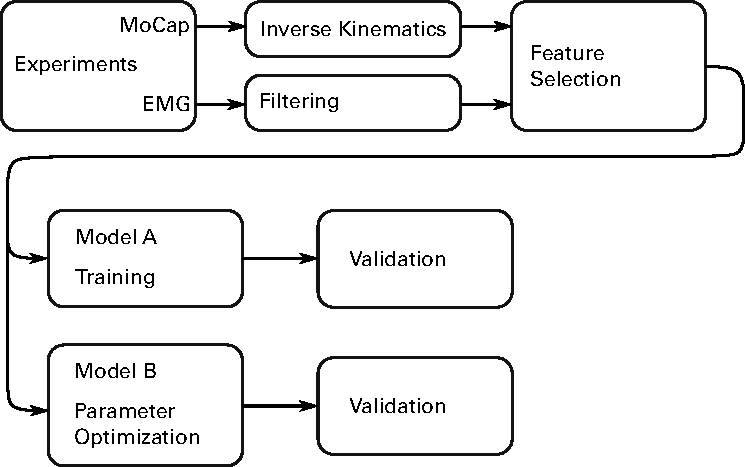
\includegraphics[width=0.8\textwidth]{images/summer_school_study/schematitc.pdf}%
  \caption{Upper Arm Movement Modeling:\\ Schematic workflow of data processing. In experiments, Motion Capture (MoCap) data and EMG signals were recorded. They were processed using inverse kinematics and filtering techniques, respectively. The size of the large datasets was reduced by selecting specific features. Those were used as training inputs for the two models A and B. The trained models were validated using a validation dataset that also originated from experiments.}%
  \label{fig:schematitc}%
\end{figure}%
%
I contributed mainly to the fields of data processing, especially filtering of EMG signals and feature selection, derivation and training of both models, A and B, their validation and the overall programming and visualization of the results. The respective fields are presented more detailed in the following, corresponding sections.

\subsection{Structure of this Chapter}
\Cref{sec:exp_study} gives an overview of the experiments, data processing and feature selection, which resulted in the required datasets. In \cref{sec:study_models}, the two models, A and B, are described. Results including the validation of the models and a discussion are given in \cref{sec:evaluation}. Conclusions follow in \cref{sec:study_conclusion}.

\section{Experimental Study}\label{sec:exp_study}

\begin{figure}%
    \centering%
    \def\svgwidth{5cm}%
    \input{images/summer_school_study/summer_school_study.pdf_tex}%
    \caption{Upper Arm Movement Modeling: \\Experimental setup for the triceps trials. The subject pulls down a rope over a pulley which is connected to a weight with mass $m_w$.
    Angles required for the kinematic formulation are the elbow angle, $\phi_e$, the forearm angle, $\phi_a$, and the angle of the weight, $\phi_w$. The length of the ulna bone is denoted by $\ell_u$.}%
    \label{fig:summer_school_study}%
\end{figure}%

Experiments are required to identify the model parameters for the particular subject. First, the experimental setup is described, then, details on the processing of the measured values are given. Then, the selection of feature points from the experimental data is described.

\subsection{Experimental Trials}

In a series of experiments, eight different actions of flexing and extending the elbow were performed by the subject. Weights of 3 kg and 5 kg were held in the hand during the elbow flexion trials. For the elbow extension trials, a pulley system was installed that redirected the force of the weight such that the downward movement of the forearm acted against the direction of the force. This is shown in \cref{fig:summer_school_study}. A detailed description of the experimental trials can be found in \cite{summerschool2019}.

Time series of position and velocity of the upper arm and the forearm were recorded using a Motion Capture system. It consisted of eight cameras that tracked three markers placed on shoulder, elbow and wrist of the subject. 

The elbow torque $\tau$ was computed as
\begin{equation*}
  \begin{array}{lll}
    \tau = m_w\,g\,\ell_u\,\sin(\phi_w) - m_{a}\,g\,\dfrac{\ell_u}{2}\,\sin(\phi_a),
  \end{array}
\end{equation*}
where $(m_w\,g)$ is the force of the weight, $m_{a}$ is the mass of forearm and hand, $\ell_u$ is the length of the ulna bone and $\phi_a$ and $\phi_w$ are the angles of the forearm and rope, as visualized in \cref{fig:summer_school_study}.

\subsection{Data Processing}
From the captured data, derived quantities of biceps ($B$) and triceps ($T$) muscles were estimated using a geometric model of the upper arm. 
The geometric model is available in the software OpenSim \cite{OpenSim2007} and was customized for the particular subject. The inverse kinematics module of OpenSim was used to estimate the muscle tendon unit lengths, $\ell_{\text{MTU},M}$, contraction velocities, $v_M=\dot{\ell}_M$, and moment arms, $r_{M}$, of the two muscles, $M\in\{B,T\}$.

EMG signals were captured by two electrodes on the skin at the biceps and triceps muscles. For both signals, several preprocessing steps were applied to obtain the inputs for the two models, A and B.

The raw signal was filtered with the same procedure as in \cite{Falisse2016}. First, a fourth-order Butterworth high pass filter with cutoff frequency 30 Hz was applied to reduce non-zero average voltages. Second, the resulting signal was full-wave rectified by taking the absolute value of every measured data point. Third, application of a fourth-order Butterworth low pass filter with 10 Hz cutoff frequency yielded a smoothed signal.
Forth, the resulting filtered EMG signals were normalized to the interval $[0,1]$, such that the value of 1 corresponds to the experimentally determined value of maximum voluntary contraction.

The measured EMG signals on the skin directly correspond to the electric excitation level $u$ in the muscle. Excitation leads to the release of free calcium ions within the sarcomere. Binding of calcium ions to myosin increases the concentration of cross-bridges. This concentration is commonly known as the muscular activation $\alpha$. The muscular activation directly corresponds to the produced force of the muscle \cite{Bayer2017}.

The concentration of free calcium ions is denoted as $\gamma$ and can be computed from the excitation $u$ by the following first order differential equation \cite{Hatze1977}
%
\begin{equation*}
  \begin{array}{lll}
    \dot{\gamma} = m\,(u - \gamma).
  \end{array}
\end{equation*}
%
We used the filtered EMG signal $u$ to obtain values for $\gamma$. \Cref{fig:emg_filtering} shows the raw and filtered EMG signals and the resulting free calcium concentration for a sample of the experimental data.

\begin{figure}%
  \centering%
  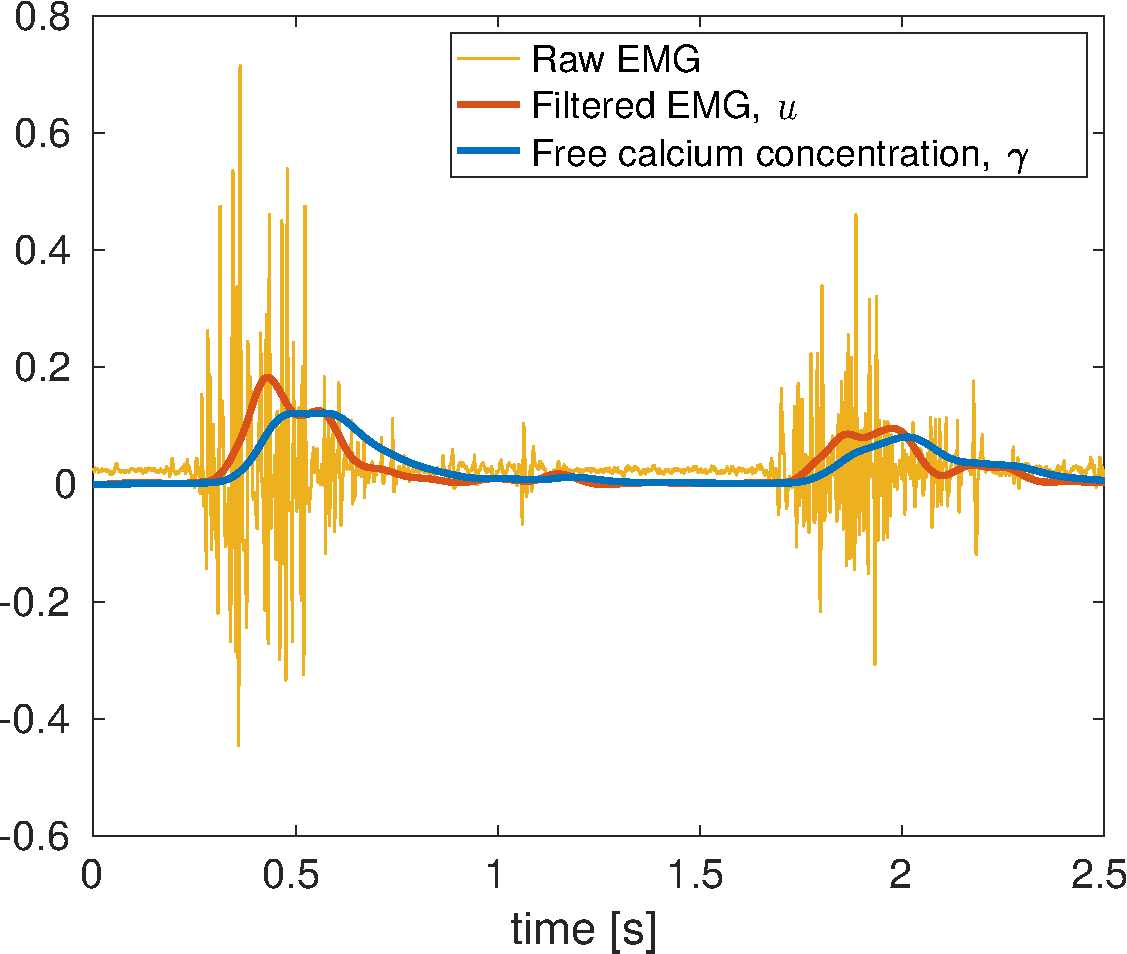
\includegraphics[width=0.8\textwidth]{images/summer_school_study/emg_filtering.pdf}%
  \caption{From raw EMG data of the biceps (yellow) to the filtered signal $u$ (red) and the free calcium concentration $\gamma$ (blue). The data are taken from the beginning of the first elbow flexion experiment. It can be seen that the filtering smooths out the initial signal and removes the constant offset. The free calcium ion concentration follows the filtered EMG with a short delay.}%
  \label{fig:emg_filtering}%
\end{figure}%

The activation of the muscle $\alpha$ does not only depend on the free ion concentration $\gamma$ but also on the current state of muscle contraction. This excitation-contraction coupling has to be described by a dynamic system of ODEs and is included in model B.
Therefore, preprocessing is completed with computing the free calcium concentration $\gamma$ and not the activation $\alpha$.

\subsection{Feature Selection} \label{sec:study_feature_selection}

The eight experimental trials were split into $n_\text{trials}=7$ experiments to be used for model identification and one for validation.
The total number $N$ of captured values in the training experiments was large, such that not all points could be used for training of models A and B.
To reduce the amount of data and, thus, speed up the computation, we selected $n \ll N$ featured values with the assumption that they are representative for the whole data set.
For every experimental trial, we choose the same fixed number $n_\text{per\_trial}$ of data points.
Our selection algorithm identifies $n_\text{per\_trial}$ timesteps, $t_i, i=1, \dots, n$ such that the summed values of the free calcium concentrations $\gamma_B(t_i) + \gamma_T(t_i)$ for biceps and triceps are evenly distributed along the value range.
This leads to $n = n_\text{trials} \cdot n_\text{per\_trial}$ selected data points.

The set of training data $\mathcal{D} = \mathcal{X} \times \mathcal{Y}$ consists of the $n$ selected vectors of the experimental values that are the input to the system of muscles, $\bfx_i \in \mathcal{X}, i=1,\dots, n$, together with the observed output values, $y_i \in \mathcal{Y}, i=1,\dots,n$.
The input vectors contain values for muscle tendon unit lengths, contraction velocities, moment arms and free calcium ion concentrations for biceps and triceps each, $\bfx_i = (\ell_{\text{MTU},B}, \ell_{\text{MTU},T}, v_B, v_T, r_{B}, r_{T}, \gamma_B, \gamma_T)^\top(t_i)$. The output values consist of the elbow torques, $y_i = \tau(t_i)$. This data set, $\mathcal{D}$, serves as training input for both models, A and B.

\section{Models}\label{sec:study_models}

The current section describes the two model approaches that can predict elbow torques from experimental input data. \Cref{sec:data_driven_model} introduces the non-parametric, data driven model A. \Cref{sec:biophysical_model} presents the biophysically based model B. It requires a parameter optimization, which is described in \cref{sec:parameter_optimization}.

\subsection{Data-driven Model A}\label{sec:data_driven_model}

The first modeling approach uses a non-parametric model. Such a model approximates the function $f$ that maps from input to output data points. The function $f$ is learned from the training data set. Regression is used to obtain predictions for new data points. In our case, we use a stochastic model that considers the probability distribution of the model function.

We use the method of \emph{Gaussian Process Regression}. A Gaussian process is a collection of random variables such that the joint distribution of every finite subset of these random variables is multivariate normal (Gaussian).
In our example, each input data point in the space of measured values, $\bfx \in \mathcal{X}$ has an associated random variable $f(\bfx)$ that describes the output of the model for this point.

A Gaussian process, $\mathcal{GP}$, is characterized by a mean function $m(\bfx)$ and a kernel function $k(\bfx,\bfx')$ that models the covariance between any pair $(\bfx, \bfx') \in \mathcal{X} \times \mathcal{X}$ of points. Different choices of kernel functions are possible and can depend on hyperparameters $\bfpsi$. Describing observed values $y$ by a Gaussian process distribution can be expressed as
\begin{equation*}
  \begin{array}{lll}
    f(x) \approx y \sim \mathcal{GP}\big(m(\bfx), k(\bfx,\bfx',\bfpsi)\big).
  \end{array}
\end{equation*}
This representation is non-parametric in the sense that no particular parametric form of the function $y=f(\bfx)$ is assumed whose (biophysical) parameters would be determined. Instead, a generic probabilistic model is constructed using the observed function values at measured inputs $\bfx_i \in \mathcal{X}$.
%More specifically, the conditional distribution $p(y|\bfx)$ considered.

Gaussian Process Regression is based on \emph{Bayesian Inference} to update a prior belief of the model to a posterior model using information contained in observations of the process.
The observed data are the set of measurements $\mathcal{D}$. 

The \emph{prior} distribution $p(\bff\mid\mathcal{X},\bfpsi)$ for the vector of function values $\bff$ is described by the Gaussian process,
\begin{equation*}
  \begin{array}{lll}
    p(\bff\mid\mathcal{X},\bfpsi) = \mathcal{N}(\bff\mid\bfm,\bfK),
  \end{array}
\end{equation*}
with mean values $\bfm = (m(\bfx_i))^\top_{i=1,\dots,n}$ and covariance matrix $\bfK$ with $K_{ij} = k(\bfx_i,\bfx_j,\bfpsi).$

The \emph{likelihood} $p(\bfy\mid f(\bfx), \bftheta)$ describes the probability of an observation $\bfy$ given a particular model $f$. The vector $\bftheta$ denotes additional parameters of the likelihood. 

Using Bayes' rule, the \emph{posterior} distribution $p(\bff\mid\mathcal{D})$ of the function values $\bff$ can be computed from prior and likelihood as
\begin{equation*}
  \begin{array}{lll}
    p(\bff\mid\mathcal{D},\bftheta,\bfpsi) 
      = \dfrac{p(\bfy\mid\bff,\bftheta)\,p(\bff\mid\mathcal{X},\bfpsi)}{p(\mathcal{D}\mid\bftheta,\bfpsi)}.
  \end{array}
\end{equation*}
This results in a measure for the uncertainty of the model $f$ at unobserved points $\bfx_\ast \notin \mathcal{D}$. 

Additionally, the fact that the measured quantities in the experiments are subject to measurement noise can be incorporated into the model.
The assumption 
\begin{equation*}
  \begin{array}{lll}
    y = f(\bfx) + \eps
  \end{array}
\end{equation*}
adds a normally distributed random variable of observational noise $\eps \sim \mathcal{N}(0,\sigma_n^2)$ to the formulation. The noise variance $\theta = \sigma_n^2$ is an additional parameter of the likelihood. 
It is also possible to explicitly model the mean function $m(\bfx)$. By replacing the model $f(\bfx)$ by $g(\bfx) = f(\bfx) + \bfh(\bfx)^\top \bfbeta$, i.e.
\begin{align*}
  %\begin{array}{rlrl}
    y &= f(\bfx) + \bfh(\bfx)^\top \bfbeta + \eps, \quad 
    &\text{ with } f(x) &\sim\mathcal{GP} \big(m(\bfx), k(\bfx,\bfx',\bfpsi)\big),\\[4mm]
    && \eps &\sim \mathcal{N}(0,\sigma_n^2),
  %\end{array}
\end{align*}
we allow for a global trend in the data that is formulated in terms of a vector of explicit basis functions $\bfh(\bfx)$ and corresponding coefficients $\bfbeta$.

The algorithm for Gaussian Process Regression involves estimating the following values from the given data during the training phase. The hyperparameters of the covariance function $\bfpsi$, the noise variance $\bftheta$, and the coefficients of the fixed basis functions $\bfbeta$ are determined by solving an optimization problem. The computation involves matrix inversions and has a computational complexity $\O(n^3)$, i.e. is cubic in the number of data points. For details, the reader is referred to the literature \cite{Rasmussen2005,kuss2006gaussian}.

In our study, training of the Gaussian Process of model A was performed using the ready to use implementation provided by MATLAB.
We parametrized the covariance by a squared exponential kernel and used constant basis functions, $\bfh(x) = 1$. We enabled observational noise, its variance $\bftheta = \sigma_n^2$ was found by optimization during training of the model.

%$p(\bff^\ast | \mathcal{D},\mathcal{X}^\ast)$
\subsection{Biophysical Model B}\label{sec:biophysical_model}

Extension of the elbow is governed by the triceps brachii muscle.
During elbow flexion, three muscles are involved: biceps brachii, brachialis and brachioradialis. For simplicity, only biceps brachii, which contributes most of the moment, is explicitly considered in the current study. The effects of the other two muscle are contained in the biceps brachii model in a lumped manner.

Thus, the biophysical model consists of two Hill-type muscle models, for biceps and triceps, respectively. The muscle models are arranged around a hinge joint for the elbow angle. The muscle forces contribute to the torque at the elbow over their respective moment arms.

Hill-type models describe the macroscopic, dynamic mechanical behavior of an entire muscle along a one-dimensional line of action.
The behavior is formulated by phenomenological, mathematical functions that have to be parametrized to fit experimental observations.

%Such models are often used to compute muscle forces in simulations of various movements, e.g. \cite{Siebert2003}, \cite{Kistemaker2006}.
Multiple variants of Hill-type models exist that use various configurations of mechanical elements to consider different properties and functionalities of the muscle. The original model was proposed in \cite{Hill1938}. It contains a contractile element (CE) and two elastic elements, arranged in series and in parallel to the CE.
The authors of \cite{Siebert2008} compare two different approaches using these three elements. The effect of tension in eccentric contractions is added to the Hill-type model by \cite{Till2008}. The authors of \cite{Gunther2007} add a forth, damping element to account for high-frequency damping of the muscle tissue. In \cite{Morl2012}, electromechanical delay is investigated with and without the additional damping element. 

\begin{figure}%
  \centering%
  \def\svgwidth{0.5\textwidth}
  \input{images/summer_school_study/hilltype.pdf_tex}%
  \caption{Mechanical structure of the Hill-type muscle model. The force generating contractile element (CE) is parallel-connected to the parallel elastic element (PEE) and connected in series to a second parallel-connected structure consisting of the serial elastic element (SEE) and the serial damping element (SDE). The length $l_\text{MTU}$ of the whole muscle tendon unit is composed of the common length $l_\text{CE}$ of CE and PEE and the common length $l_\text{SEE}$ of SEE and SDE. The variable $l_\text{CE}$ is an internal state of the model.}
  \label{fig:hilltype}%
\end{figure}%

\newcommand{\CE}{\text{CE}}
\newcommand{\MTU}{\text{MTU}}

We employ the four-element Hill-type muscle model that is described by \cite{Hilltype2014}. Its structure is visualized in \cref{fig:hilltype}. It consists of four components: the contractile element (CE), the parallel elastic element (PEE), the serial elastic element (SEE), and the serial damping element (SDE). Inputs to the model are the muscular activation $\alpha(t)$, the length $l_\MTU(t)$ and the contraction velocity $\dot{l}_\MTU(t)$ of the muscle tendon unit (MTU).
The output of the model is the muscle force $f_\text{MTU}(t)$. The model contains one internal state variable, the length $l_\text{CE}(t)$ of the CE. The muscle dynamics determine this internal length and its time derivative, the contraction velocity $\dot{l}_\text{CE}(t)$ of the CE.

The resulting force of the MTU is given as sum of the forces of the respective parallel elements as visualized in \cref{fig:hilltype}:
\begin{equation}\label{eq:hill_type0}
  \begin{array}{lll}
    F_\MTU = F_\CE(l_\CE, \dot{l}_\CE, \alpha) + F_\text{PEE}(l_\CE) = F_\text{SEE}(l_\CE,l_\MTU) + F_\text{SDE}(l_\CE,\dot{l}_\CE,\dot{l}_\MTU,\alpha).
  \end{array}
\end{equation}
The force terms of the four elements, $F_\CE, F_\text{PEE}, F_\text{SEE}$ and $F_\text{SDE}$ are described by analytical functions that use a total of 19 parameters. A description of the detailed equations and parameters can be found in \cite{Hilltype2014}. In the following, an overview over the formulation is given with a focus on the piecewise formulated terms that contribute to the overall muscle model. In the following formulations, underlined variables designate constant parameters that either have to be specified or follow from other given parameters.

The muscle output force $F_\text{MTU}$ is computed by the second identity of \cref{eq:hill_type0}, i.e., from the forces $F_\text{SEE}$ and $F_\text{SDE}$. The force $F_\text{SEE}$ acting in the SEE is formulated as a continuous piecewise function with a constant zero, an exponential and a linear branch:
\begin{equation*}
  \begin{array}{lll}
    F_\text{SEE}(\ell_\CE,\ell_\MTU) = \begin{cases}
      0, & \ell_\text{SEE} < \underline{l_{\text{SEE},0}}\\[2mm]
      \underline{K_\text{SEE,nl}}(\ell_\text{SEE} - \underline{\ell_\text{SEE,0}})^{\underline{\nu_\text{SEE}}}, & \ell_\text{SEE} < \underline{\ell_\text{SEE,nll}}\\[2mm]
    \underline{\Delta F_\text{SEE,0}} + \underline{K_\text{SEE,l}}(\ell_\text{SEE} - \underline{\ell_\text{SEE,nll}}), & 
    \ell_\text{SEE} \geq \underline{\ell_\text{SEE,nll}}
    \end{cases}, \quad \text{with } \ell_\text{SEE} = \ell_\MTU - \ell_\CE.
  \end{array}
\end{equation*}

The damping force $F_\text{SDE}$ in the SDE is proportional to the lengthening velocity ${\dot{\ell}_\text{SEE} = \dot{\ell}_\MTU - \dot{\ell}_\CE}$ of this element. It is given by
\begin{equation}\label{eq:sde_force}
  \begin{array}{lll}
    F_\text{SDE}(l_\CE,\dot{l}_\CE,\dot{l}_\MTU,\alpha) \\ \qquad = \underline{D_\text{SDE,max}}\left( (1-\underline{R_\text{SDE}}) \dfrac{F_\text{PEE}(\ell_\CE)+F_\text{CE}(\ell_\CE, \dot{\ell}_\CE, \alpha)}{\underline{F_\text{max}} + \underline{R_\text{SDE}}} \right) (\dot{\ell}_\MTU - \dot{\ell}_\CE).
  \end{array}
\end{equation}
The amount of damping is dependent on the force $F_\MTU$ of the MTU which appears in the nominator of the fraction in \cref{eq:sde_force} as the sum of the forces $F_\text{PEE}$ and $F_\CE$. Formulas for these two forces are given in the following.

The force $F_\text{PEE}$ of the PEE is formulated piecewise as a shifted and cut off polynomial function:
\begin{equation}\label{eq:fpee}
  \begin{array}{lll}
    F_\text{PEE}(\ell_\CE) = \begin{cases}
      0, & \ell_\CE < \underline{\ell_{\text{PEE},0}}\\[4mm]
    \underline{K_\text{PEE}}(l_\CE - \underline{l_{\text{PEE},0}})^{\underline{\nu_\text{PEE}}},& \ell_\CE \geq \underline{\ell_{\text{PEE},0}}
    \end{cases}.
  \end{array}
\end{equation}

The force $F_\CE$ of the CE is the active force produced by the muscle and is given by:
\begin{equation}\label{eq:fce}
  \begin{array}{lll}
    F_\CE(l_\CE, \dot{l}_\CE, \alpha) 
    = \underline{F_\text{max}} \left(
    \dfrac{\alpha\,F_\text{isom}(\ell_\CE) + A_\text{rel}(\dot{\ell}_\CE,\ell_\CE,\alpha)}
    {1 - 
    \frac{\dot{\ell}_\CE}
    {B_\text{rel}(\dot{\ell}_\CE,\ell_\CE,\alpha)\,\ell_{\CE,\text{opt}}}}\right)
    - A_\text{rel}(\dot{\ell}_\CE,\ell_\CE,\alpha).
  \end{array}
\end{equation}
It can be seen that the active force depends on the activation level $\alpha$. 
The formulation of $F_\CE$ contains the two main characteristic curves for muscle forces, the force-length relation and the force-velocity relation.

The force-length relation is modeled by the function $F_\text{isom}(\ell_\CE)$ of isometric force, which describes the relative force for the condition $\dot{\ell}_\CE = 0$. This function is formulated piecewise for CE lengths $\ell_\CE$ smaller and larger than an optimal length $\ell_\text{CE,opt}$. 

The force-velocity relation follows from the auxiliary functions $A_\text{rel}(\dot{\ell}_\CE,\ell_\CE,\alpha)$ and $B_\text{rel}(\dot{\ell}_\CE,\ell_\CE,\alpha)$. These functions have different forms for concentric ($\dot{\ell}_\CE < 0$) and eccentric ($\dot{\ell}_\CE \geq 0$) conditions as well as for the two ranges of CE  length, $\ell_\CE < \ell_\text{CE,opt}$ and $\ell_\CE \geq \ell_\text{CE,opt}$.

\begin{figure}%
  \centering%
  \begin{subfigure}[t]{0.9\textwidth}%
    \centering%
    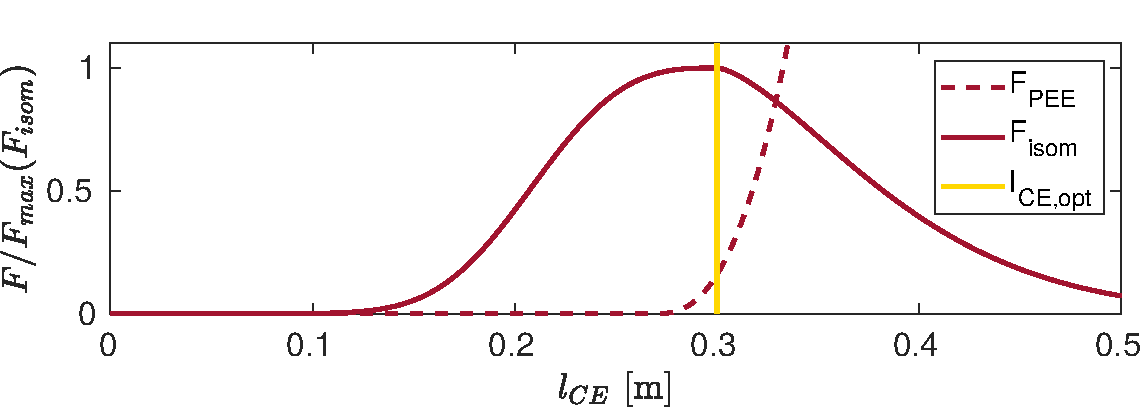
\includegraphics[width=\textwidth]{images/summer_school_study/force_curves_generic_length.pdf}%
    \caption{Force-length curves of the PEE (dashed red line) and isometric force $F_\text{isom}$ (solid red line) for an isometric condition ($\dot{l}_\CE=0$), normalized to the maximum isometric force. The optimal length $l_\text{CE,opt}$ of the CE is shown as yellow vertical line. The force $F_\text{PEE}(l_\CE)$ of the PEE is zero for $l_\CE < 0.9\,l_\text{CE,opt}$. The isometric contraction force $F_\text{isom}$ is formulated piecewise by two branches separated by $l_\text{CE,opt}$.}%
    \label{fig:force_curves_generic_length}%
  \end{subfigure}\\[6mm]
  \begin{subfigure}[t]{0.9\textwidth}%
    \centering%
    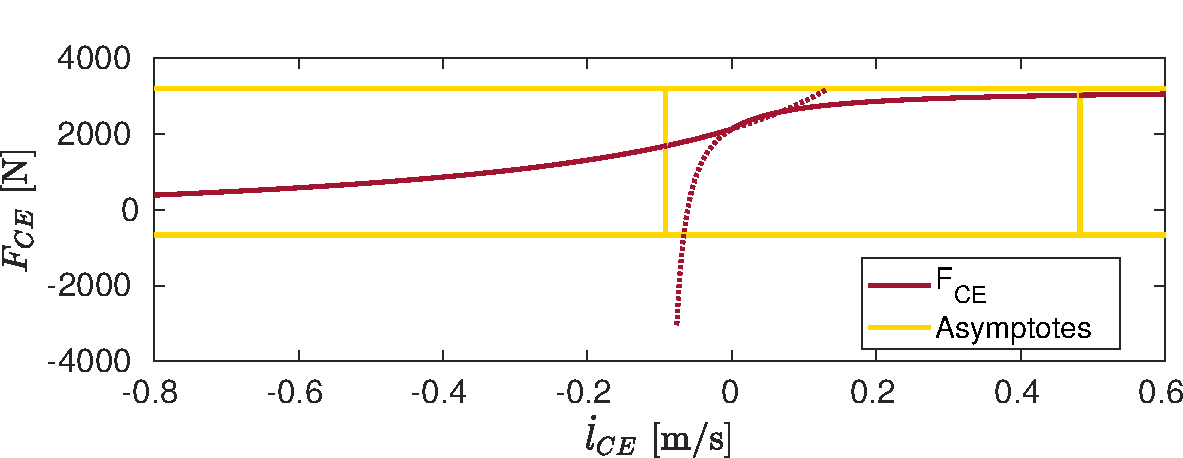
\includegraphics[width=\textwidth]{images/summer_school_study/force_curves_generic_velocity.pdf}%
    \caption{Force-velocity curve $F_\CE(\dot{l}_\CE)$ of the CE at optimal length $l_\CE=l_{\CE,\text{opt}}$, and for activation level $\alpha=0.5$. The function (red solid line) is formulated piecewise, graphs of the base functions of the two branches continue as red dotted lines. Their limits and singularities are visualized by the yellow horizontal and vertical asymptotes.}%
    \label{fig:force_curves_generic_velocity}%
  \end{subfigure}%
  \caption{Force-length and force-velocity relations for the muscle model with generic parameters taken from literature \cite{Hilltype2014}.}%
  \label{fig:force_curves_generic}%
\end{figure}%

\Cref{fig:force_curves_generic} visualizes the two main characteristic curves of the model. 
\Cref{fig:force_curves_generic_length} shows how the generated force depends on the length of the CE. 
The active force $F_\CE$, given by \cref{eq:fce}, is visualized by the solid red line. It has its maximum at the optimal length $l_\text{CE,opt}$ of the CE. This can be explained by the overlap of actin and myosin filaments in the sarcomere. The overlap is lower when the actin filaments are pulled apart or pushed together. A higher overlap leads to a higher force output.

The dashed line in \cref{fig:force_curves_generic_length} represents the passive force $F_\text{PEE}$ of the elastic muscular tissue, formulated in \cref{eq:fpee}. The passive force is essentially generated by the titin proteins in the sarcomere. Only starting from a certain length, the structure exerts reaction forces against lengthening forces to avoid overstretching of the muscle.

\cref{fig:force_curves_generic_velocity} shows the force-velocity relation of the Hill-type model. The curve of $F_\CE(\dot{l}_\CE)$ is composed of two branches: 
The concentric branch for shortening contraction with $\dot{l}_\CE \leq 0$ and the eccentric branch for lengthening contraction with $\dot{l}_\CE > 0$. It can be seen that the generated force increases monotonically over the lengthening velocity. It approaches a limit for maximum positive and negative velocity. These limits can be adjusted by parameters of the model and are exemplary for how the shape of the curves of a Hill-type model can be parametrized.

In addition to the resulting muscle force $F_\MTU$, a formulation for the internal state variable $\ell_\CE$ is required.
The second identity of \eqref{eq:hill_type0} can be solved for the lengthening velocity $\dot{\ell}_\CE$ of the CE to get an evolution equation for the length $\ell_\CE$ of the CE. The derivation and the resulting formula can be found in \cite{Hilltype2014}.

To describe the activation dynamics, i.e., the evolution of the muscle activation ${\alpha \in [0,1]}$, the model of Hatze et al. \cite{Hatze1977} is used.
The activation is computed depending on the free calcium ion concentration $\gamma$ and the length $\ell_\CE$ of the CE by
\begin{equation*}
  \begin{array}{lll}
    \alpha(\ell_\CE,\gamma) = \dfrac{\underline{a_0} + \big(\rho(\ell_\CE)\,\gamma\big)^3}
    {1 + \big(\rho(\ell_\CE)\,\gamma\big)^3}.
  \end{array}
\end{equation*}
The function $\rho$ is given by
\begin{equation*}
  \begin{array}{lll}
    \rho(\ell_\CE) = \underline{c}\,\underline{\eta}\,\dfrac{(\underline{k}-1)\,\ell_\CE}{(\underline{k} - \ell_\CE/\ell_\text{CE,opt})\,l_\text{CE,opt}}.
  \end{array}
\end{equation*}
All used parameter values for the activation dynamics can be found in \cite{Bayer2017}.

In summary, we get the following coupled system of differential-algebraic equations, where $f_\CE$ and $f_\alpha$ denote the respective formulas:
\begin{align}
  F_\MTU &= F_\MTU(\ell_\MTU,l_\CE,\dot{l}_\CE,\alpha),      \label{eq:hill_type1} \\[4mm]
  \dot{l}_\CE &= f_\CE(l_\CE,\ell_\MTU,\dot{l}_\MTU,\alpha), \label{eq:hill_type2}\\[4mm]
  \alpha &= f_\alpha(\gamma, l_\CE).                      \label{eq:hill_type3}
\end{align}

To compute the joint torque in a system of an agonist and antagonist muscle pair, two instances of the presented Hill-type muscle model can be used. In our study considering the upper arm, the torque $\tau$ at the elbow is computed by multiplying the predicted forces $F_{\MTU,B}$ and $F_{\MTU,T}$ of biceps and triceps with the corresponding moment arms $\hat{r}_B$ and $\hat{r}_T$:
\begin{equation}\label{eq:muscle_torque}
  \begin{array}{lll}
    \tau = F_{\MTU,B}(l_{\MTU,B},\dot{l}_{\MTU,B},\alpha_B) \cdot \hat{r}_B - F_{\MTU,T}(l_{\MTU,T},\dot{l}_{\MTU,T},\alpha_T) \cdot \hat{r}_T.
  \end{array}
\end{equation}

\subsection{Parameter Identification for Model B}\label{sec:parameter_optimization}
%
The process of model identification finds the parameters that make the model B predict correct values for the specific subject, i.e., minimizes the error in the predicted outcome for the training data set.

The following minimization is performed:
\begin{align}
  &&\min\limits_{\substack{\bftheta_M,l_{\CE,M}(t), \\\forall M \in \{B,T\}, \,\forall t \in \mathcal{T}}} &\sum\limits_{t\in \mathcal{T}}|\tau(t) - \hat{\tau}(t)|^2
   \label{eq:opt_1}\\[4mm]
  &&\text{s.t. }\forall t \in \mathcal{T}:\quad &\tau(t) = F_{\MTU,B}(t,l_{\CE,B},\bftheta_B) \cdot \hat{r}_B(t) \notag\\
      &&&\qquad\quad- F_{\MTU,T}(t,l_{\CE,T},\bftheta_T) \cdot \hat{r}_T(t),                 \label{eq:opt_2}\\[4mm]
  &&& \dot{l}_{\CE,M}(t) = \dot{\hat{l}}_{\MTU,M}(t),\quad M \in \{B,T\},      \label{eq:opt_3}\\[4mm]
  &&& \bftheta_B, \bftheta_T \in \Theta,                                       \label{eq:opt_4}\\[4mm]
  &&& l_{\CE,M}(t) \in [0,l_{\MTU,M}(t)],\quad M \in \{B,T\}.                  \label{eq:opt_5}
\end{align}

The optimization variables are the parameters $\bftheta_B$ and $\bftheta_T$ for the biceps and triceps Hill-type models and the lengths $l_{\CE,B}(t)$ and $l_{\CE,T}(t)$ of the contractile elements for both models at every point in time. The variables designated as $\hat{\square}$ are the measured quantities from the training experiments. The objective function given in \cref{eq:opt_1} penalizes the difference between computed torque $\tau$ and measured torque $\hat{\tau}$ at every timestep $t \in \mathcal{T}$ of the training data. 

\Cref{eq:opt_2} computes the torque values and follows from \cref{eq:muscle_torque} of the muscle model. For every point in time, the predicted forces $F_{\MTU,B}$ and $F_{\MTU,T}$ are multiplied with the measured moment arms $\hat{r}_B$ and $\hat{r}_T$.

In \cref{eq:opt_3}, the contraction velocities are constrained to the measured values. Because the lengthening velocity $\dot{l}_\CE$ of the CE is an internal quantity and, thus, cannot be observed in experiments, we assume it to be equal to the lengthening velocity of the whole muscle: $\dot{l}_\CE \approx \dot{l}_{\MTU} = \dot{l}_\text{CE} + \dot{l}_\text{SEE}$. This requires the assumption $\dot{l}_{\text{SEE}} \approx 0$ which can be justified given the low dynamic nature of the experiments.

By \cref{eq:opt_4}, we bound each of the parameters $\bftheta_B$ and $\bftheta_T$ to a range between half and twice the generic value from literature.
The lengths of the CEs are constrained by \cref{eq:opt_5} to be positive and smaller than the length of the MTU.

All optimization variables are normalized to improve the numerical conditioning of the optimization problem. 
The parameters $\bftheta_B$ and $\bftheta_T$ are normalized with respect to generic values from literature that were taken from \cite{Gunther2007, Morl2012, Hilltype2014}. The initial values are set to one, which corresponds to the generic literature values.
The internal states $l_{\CE,B}$ and $l_{\CE,T}$, are normalized with respect to the measured MTU lengths $\hat{l}_{\MTU,B}$ and $\hat{l}_{\MTU,T}$ and initialized with zero.

%For training of model B, the optimization problem for the parameters needed to be solved. 
We implemented the Hill-type models and the constraints in MATLAB and used the nonlinear programming implementation, \code{fmincon}, to minimize the given bounded and nonlinear constrained, multivariable function.
In our study, the total number of optimization variables is computed by $2\cdot 19 + 2n = 598$, as each of the parameter vectors $\bftheta_B,\bftheta_T$ had 19 entries. 

\section{Results and Discussion}\label{sec:evaluation}

In the following, results of connecting the two model formulations, A and B, to the experimental data are presented.
At first, \cref{sec:res_feature_selection} gives details on the preprocessed data. The training phase is described in \cref{sec:res_training}. Applying the trained models to the validation data is done in \cref{sec:res_validation}. Then, \cref{sec:res_simplified_a} tests a simplified version for model A. Then, \cref{ref:res_insights_b} shows some insights into the optimized parameter values for model B.

\subsection{Feature Selection}\label{sec:res_feature_selection}
% intro
The experimental data is split into a training and a validation dataset. \Cref{fig:selected_points} shows the processed data of the training data set. In total, we captured $N=\num{34934}$ data points for the seven experimental trials. Out of these, we select $n_\text{per\_trial}=\num{40}$ feature points in every trial, leading to a total of $n=n_\text{per\_trial}\cdot n_\text{trials}=\num{280}$ points. The selected points are visualized by crosses in the top plot of \cref{fig:selected_points}. It can be seen that the algorithm described in \cref{sec:study_feature_selection} distributes the feature points equally along the $\gamma$ axis.

\begin{figure}%
  \centering%
  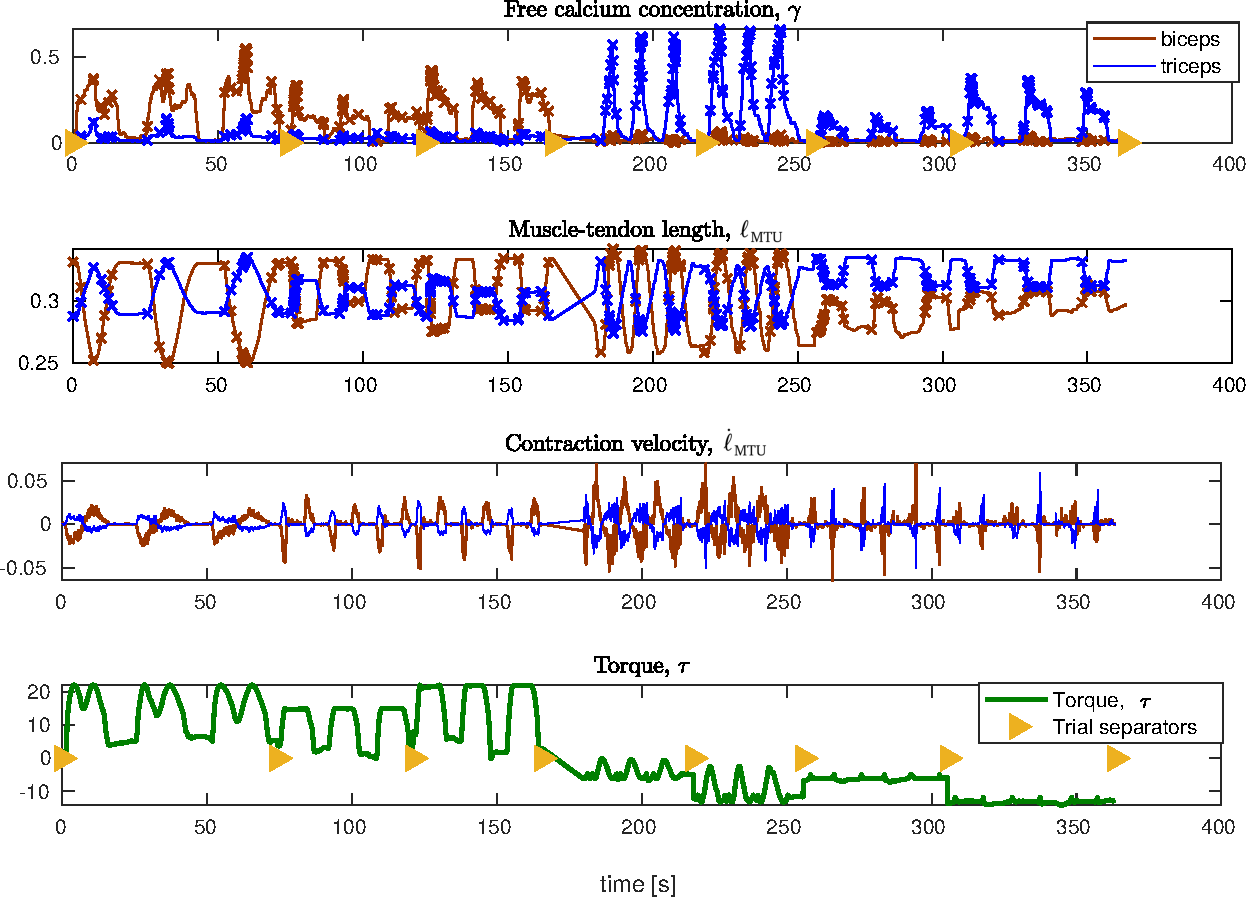
\includegraphics[width=\textwidth]{images/summer_school_study/selected_points.pdf}%
  \caption{Processed experimental values over time that were used for training of both models. The concatenated data of seven trials are shown, which yield an end time of $\SI{363.32}{s}$. The individual trials are separated by the yellow triangles on the $x$-axis. The three upper plots show the values of $\gamma, \ell_\MTU$ and $\dot{l}_\MTU$ for both biceps (brown) and triceps (blue), the bottom plot shows the elbow torque $\tau$. The selected feature points are visualized as crosses in the two top plots. In the upper-most plot, it can be seen that the first three trials, which correspond to elbow flexion, mainly activated the biceps muscle, whereas in the last four trials, corresponding to elbow extension, the triceps is more active.
}%
  \label{fig:selected_points}%
\end{figure}%

\subsection{Training of the Models}\label{sec:res_training}
%
Training of model A consists of estimating the hyperparameters for the Gaussian Process Regression model from the training data.

For model B, the optimization problem for the biophysical parameters is solved. The resulting parameter values and their relation to the initial values are summarized in \cref{tab:model_b_parameters}. It can be seen that none of the final parameter values is limited by the constraints, which would be $\SI{-50}{\percent}$ and +\SI{100}\percent. However, it was observed that including the constraints helps the optimizer to stay in the valid range of meaningful model parameters and, thus, reach the optimum faster.

\begin{table}[t] 
  \centering
  %\begin{scriptsize}
  
    \begin{tabular}{@{}llllll@{}}
%\hline
 %| param              | biceps   |            | triceps  |            %|
 %| ------------------ | -------- | ---------- | -------- | ---------- %|
 %| CE_F_max           | +11.03 % | 4729.97    | -49.04 % | 2171.04    |
 %| CE_l_CEopt         | +31.72 % | 0.40       | -25.36 % | 0.22       |
 %| CE_DeltaW_limb_des | +10.86 % | 0.39       | +10.86 % | 0.39       |
 %| CE_DeltaW_limb_asc | +91.61 % | 0.67       | +5.05 %  | 0.37       |
 %| CE_v_CElimb_des    | +10.86 % | 1.66       | +10.86 % | 1.66       %|
 %| CE_v_CElimb_asc    | -46.39 % | 1.61       | +95.87 % | 5.88       |
 %| CE_A_rel0          | +14.03 % | 0.29       | -20.34 % | 0.20       |
 %| CE_B_rel0          | +77.51 % | 3.99       | +41.38 % | 3.18       |
 %| CE_S_eccentric     | -4.12 %  | 1.92       | +22.92 % | 2.46       |
 %| CE_F_eccentric     | -30.94 % | 1.04       | +36.79 % | 2.05       |
 %| PEE_L_PEE0         | +10.86 % | 1.00       | +10.86 % | 1.00       |
 %| PEE_l_PEE0         | +10.86 % | 0.30       | +10.86 % | 0.30       |
 %| PEE_v_PEE          | +10.86 % | 2.77       | +10.86 % | 2.77       |
 %| PEE_F_PEE          | +10.86 % | 2.22       | +10.86 % | 2.22       |
 %| PEE_K_PEE          | +10.86 % | 1410470.38 | +10.86 % | 1410470.38 |
 %| SDE_D_SE           | +10.86 % | 0.33       | +10.86 % | 0.33       |
 %| SDE_R_SE           | +8.63 %  | 0.01       | -10.99 % | 0.01       |
 %| SDE_d_SEmax        | +8.41 %  | 513.16     | -10.64 % | 422.98     |
 %| SEE_l_SEE0         | -24.95 % | 0.13       | -10.28 % | 0.15       |
 %| SEE_DeltaU_SEEnll  | +59.16 % | 0.07       | +23.58 % | 0.05       |
 %| SEE_DeltaU_SEEl    | +63.34 % | 0.03       | +19.02 % | 0.02       |
 %| SEE_DeltaF_SEE0    | -42.40 % | 327.16     | +64.75 % | 935.78     |
 
% contractile element (CE)
%===========================
%  CE_F_max                         % F_max in [N] for Extensor (Kistemaker et al., 2006)
%  CE_l_CEopt                       % optimal length of CE in [m] for Extensor (Kistemaker et al., 2006)
%* CE_DeltaW_limb_des = 0.35;       % width of normalized bell curve in descending branch (Moerl et al., 2012)
%* CE_DeltaW_limb_asc = 0.35;       % width of normalized bell curve in ascending branch (Moerl et al., 2012)
%* CE_v_CElimb_des = 1.5;           % exponent for descending branch (Moerl et al., 2012)
%  CE_v_CElimb_asc = 3.0;           % exponent for ascending branch (Moerl et al., 2012)
%* CE_A_rel0 = 0.25;                % parameter for contraction dynamics: maximum value of A_rel (Guenther, 1997, S. 82)
%* CE_B_rel0 = 2.25;                % parameter for contraction dynmacis: maximum value of B_rel (Guenther, 1997, S. 82)
%  eccentric force-velocity relation:
%* CE_S_eccentric  = 2;             % relation between F(v) slopes at v_CE=0 (van Soest & Bobbert, 1993)
%  CE_F_eccentric  = 1.5;           % factor by which the force can exceed F_isom for large eccentric velocities (van Soest & Bobbert, 1993)

% paralel elastic element (PEE)
%===============================
%  PEE_L_PEE0   = 0.9;                               % rest length of PEE normalized to optimal lenght of CE (Guenther et al., 2007)
%  PEE_v_PEE    = 2.5;                               % exponent of F_PEE (Moerl et al., 2012)
%  PEE_F_PEE    = 2.0;                               % force of PEE if l_CE is stretched to deltaWlimb_des (Moerl et al., 2012)

% serial damping element (SDE)
%=============================
%* SDE_D_SE    = 0.3;               % xxx dimensionless factor to scale d_SEmax (Moerl et al., 2012)
%* SDE_R_SE    = 0.01;              % minimum value of d_SE normalised to d_SEmax (Moerl et al., 2012)
%  SDE_d_SEmax = SDE_D_SE*(CE_F_max*CE_A_rel0)/(CE_l_CEopt*CE_B_rel0);
                                    % maximum value in d_SE in [Ns/m] (Moerl et al., 2012)

% serial elastic element (SEE)
% ============================
%  SEE_l_SEE0        = 0.172;       % rest length of SEE in [m] (Kistemaker et al., 2006)
%  SEE_DeltaF_SEE0   = 568;         % both force at the transition and force increase in the linear part in [N] (~ 40% of the maximal isometric muscle force)
%  SEE_DeltaU_SEEnll = 0.0425;      % relativ stretch at non-linear linear transition (Moerl et al., 2012)
%* SEE_DeltaU_SEEl   = 0.017;       % relativ additional stretch in the linear part providing a force increase of deltaF_SEE0 (Moerl, 2012)
% 
     \toprule
    \textbf{CE} 
      & $F_{\mathrm{max}}\,[\mathrm{N}]$
      & $l_{\mathrm{CE},opt}\,[\mathrm{m}]$ 
      & $\Delta W_{d} \,[\;]$ 
      & $\Delta W_{a} \,[\;]$ 
      & $\nu_{\mathrm{CE},d} \,[\;]$ \\  \midrule
    Generic & $4260$ & $0.3$ & $0.35$ & $0.35$ & $1.5$  \\ %\hline
    Biceps  & $+\SI{11.0}{\percent}$ & $+\SI{31.7}{\percent}$ & $+\SI{10.9}{\percent}$ & $+\SI{91.6}{\percent}$ & $+\SI{10.9}{\percent}$  \\ %\hline
    Triceps & $-\SI{49.0}{\percent}$ & $-\SI{25.4}{\percent}$ & $+\SI{10.9}{\percent}$ & $+\SI{5.1}{\percent}$ & $+\SI{10.9}{\percent}$  \\ %\hline 
    \addlinespace[2ex]
    \textbf{CE} 
      &  $\nu_{\mathrm{CE},a} \,[\;]$ 
      & $A_\text{rel,0} \,[\;]$  
      & $B_\text{rel,0} \,[\;]$ 
      & $S_\text{ecc} \,[\;]$ 
      & $F_\text{ecc} \,[\;]$\\  \hline
    Generic & $3.0$ & $0.25$ & $2.25$ & $2$ & $1.5$ \\ %\hline
    Biceps & $-\SI{46.4}{\percent}$ & $+\SI{14.0}{\percent}$ & $+\SI{77.5}{\percent}$ & $-\SI{4.1}{\percent}$ & $-\SI{30.1}{\percent}$ \\ %\hline
    Triceps &  $+\SI{95.9}{\percent}$ & $-\SI{20.3}{\percent}$ & $+\SI{41.4}{\percent}$ & $+\SI{22.3}{\percent}$ & $+\SI{36.8}{\percent}$ \\ %\hline
    \addlinespace[2ex]
    \textbf{PEE} 
      & $L_{\mathrm{PEE},0} \,[\;]$ 
      & $\nu_{\mathrm{PEE}} \,[\;]$ 
      & $F_{\mathrm{PEE}} \,[\;]$
      \\ \hline
    Generic & $0.9$ & $2.5$ & $2.0$  \\ %\hline
    Biceps & $+\SI{10.9}{\percent}$ & $+\SI{10.9}{\percent}$ & $+\SI{10.9}{\percent}$  \\ %\hline
    Triceps & $+\SI{10.9}{\percent}$ & $+\SI{10.9}{\percent}$ & $+\SI{10.9}{\percent}$  \\ %\hline
    \addlinespace[2ex]
    \textbf{SDE} 
      & $D_{\mathrm{SDE}} \,[\;]$ 
      & $R_{\mathrm{SDE}} \,[\;]$ 
      \\ \midrule
    Generic & $0.3$ & $0.01$    \\ %\hline
    Biceps & $+\SI{10.9}{\percent}$ & $+\SI{8.6}{\percent}$   \\ %\hline
    Triceps & $+\SI{10.9}{\percent}$ & $-\SI{11.0}{\percent}$  \\ %\hline
    \addlinespace[2ex]
    \textbf{SEE} 
      & $l_{\mathrm{SEE},0}\,[\mathrm{m}]$ 
      & $\Delta F_{\mathrm{SEE},0} \,[\;]$  
      & $\Delta U_\text{l} \,[\;]$  
      & $\Delta U_\text{nll}\,[\;]$
      \\ \hline
    Generic & $0.172$ & $0.0425$ & $0.017$ & $568$ \\ %\hline
    Biceps & $-\SI{25.0}{\percent}$ & $-\SI{42.4}{\percent}$ & $+\SI{63.3}{\percent}$ & $+\SI{59.2}{\percent}$ \\ %\hline
    Triceps & $-\SI{10.3}{\percent}$ & $+\SI{64.75}{\percent}$ & $+\SI{19.0}{\percent}$ & $+\SI{23.6}{\percent}$ \\ %\hline
    \bottomrule
  \end{tabular}

  \caption{Hill-type muscle model parameters of the four elements: CE, PEE, SDE and SEE, initial values given in literature and relative changes of the optimized values. Further explanations of the parameters and references to literature containing their initial values are given in \cite{Hilltype2014}.}
  \label{tab:model_b_parameters}
  %\end{scriptsize}
\end{table}

After training of the models A and B using the selected points of the training dataset, both models were tested by a \emph{resubstitution prediction}, i.e., predicting output from the training input data. The results are shown in \cref{fig:measured_optimized_torque_A} for model A and \cref{fig:measured_optimized_torque_B} for model B. As this evaluation only uses the subset of selected experimental values, the data points have no natural ordering. They were sorted for better visibility.

It can be seen that, for both models, the predicted values are a good fit to the measured values. For model A, the predicted 95\% confidence interval includes the actually measured values almost everywhere. For model B, the predicted values show a higher variance, especially for high torque values.

\begin{figure}%
  \centering%
  \begin{subfigure}[t]{0.48\textwidth}%
    \centering%
    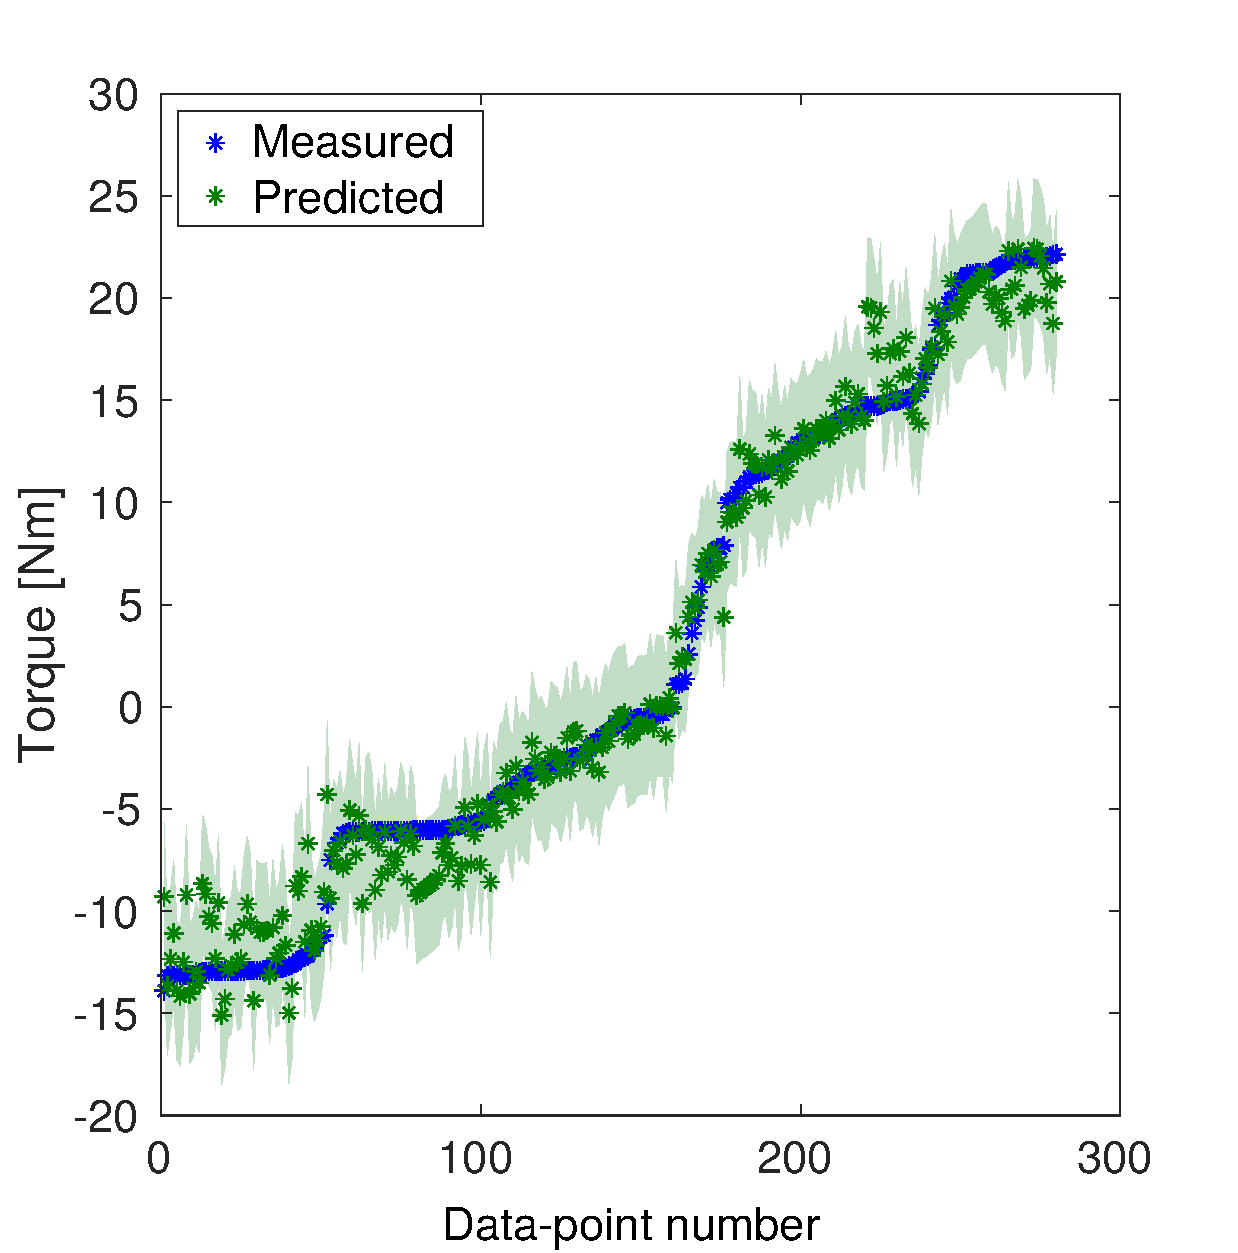
\includegraphics[width=\textwidth]{images/summer_school_study/measured_optimized_torque_A.pdf}%
    \caption{Measured values (blue) and values predicted by model A (dark green), with 95\% confidence interval (light green).}%
    \label{fig:measured_optimized_torque_A}%
  \end{subfigure}%
  \quad
  \begin{subfigure}[t]{0.48\textwidth}%
    \centering%
    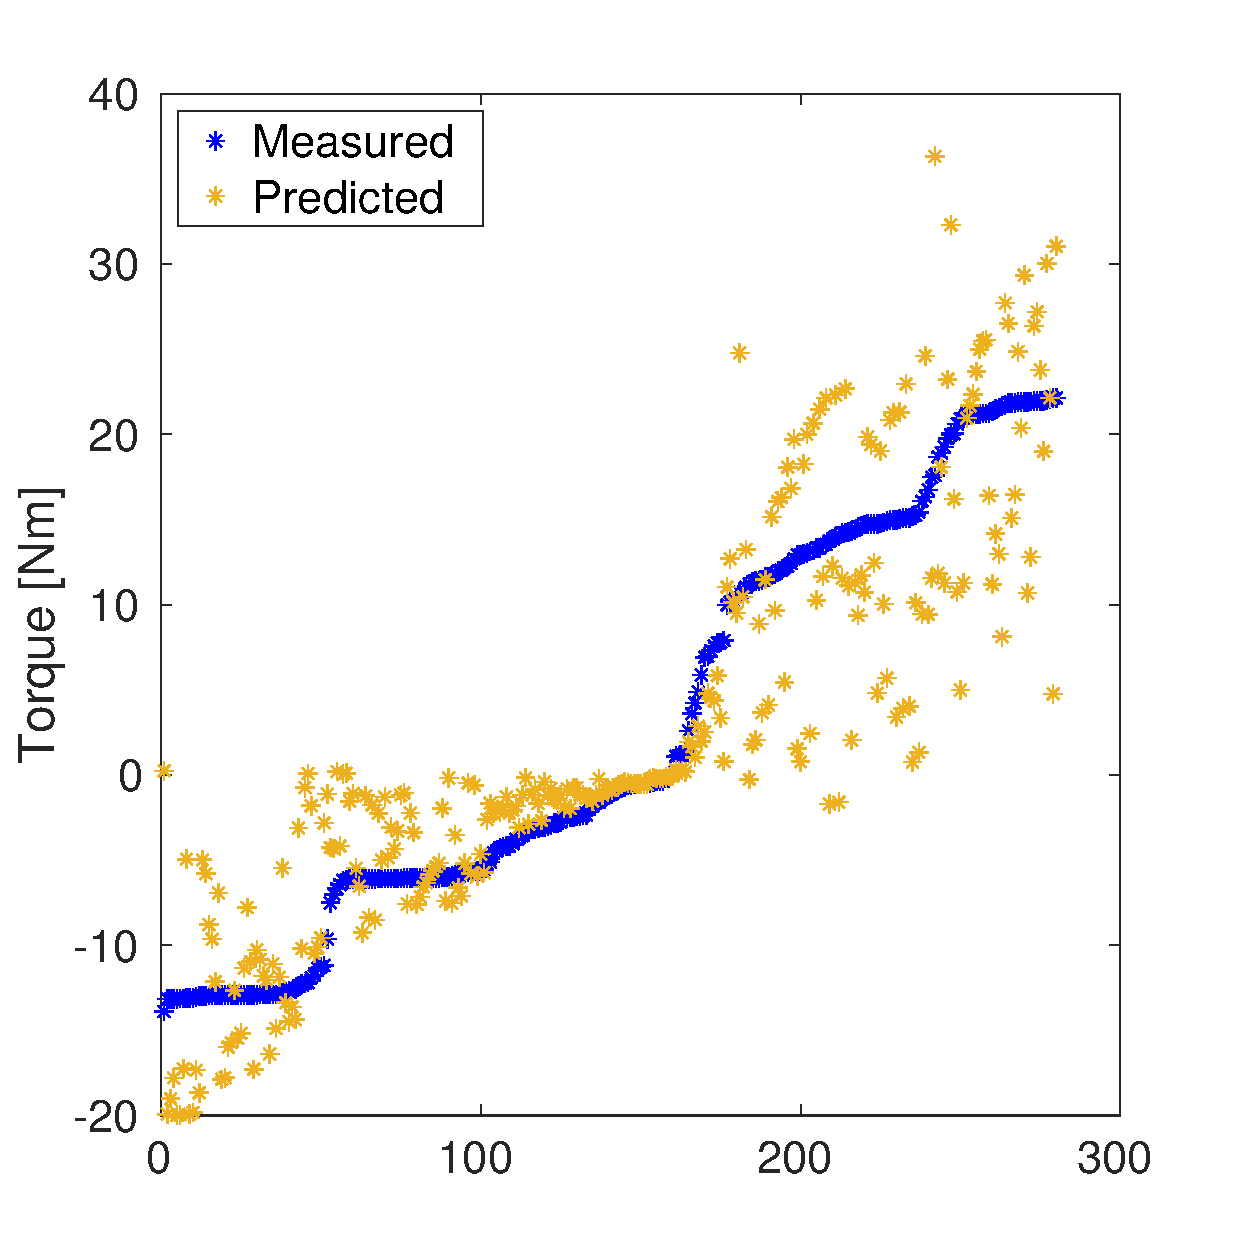
\includegraphics[width=\textwidth]{images/summer_school_study/measured_optimized_torque_B.pdf}%
    \caption{Measured values (blue) and values predicted by model B (orange).}%
    \label{fig:measured_optimized_torque_B}%
  \end{subfigure}%
  \caption{Resubstitution prediction: Measured and predicted torque values for the training data set. The measured points are ordered and numbered by magnitude, the order of the predicted points matches the order of the measured points.}%
  \label{fig:measured_optimized_torque}%
\end{figure}%

\subsection{Validation}\label{sec:res_validation}

The next evaluation uses the validation dataset and compares the predicted outputs of the models with the actual experimental values.
In contrast to the training data, where a small number $n$ of points was selected, we now use all captured values. This involves a total of \num{54e3} data points for a time span of $t=\SI{54}s$. 

\begin{figure}%
  \centering%
  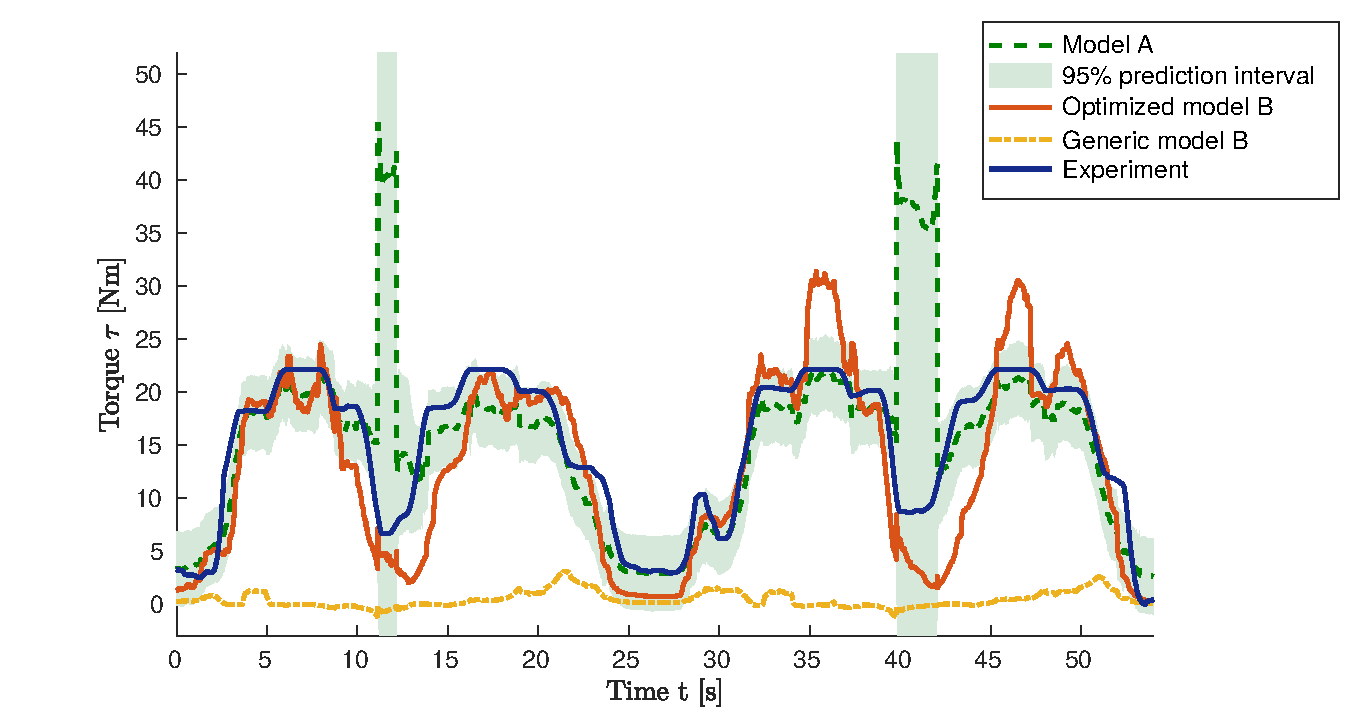
\includegraphics[width=\textwidth]{images/summer_school_study/validation_bv5_40_points.pdf}%
  \caption{Validation: Predicted torque values by model A (green), trained model B (red) and untrained model B (yellow), in comparison to the experimentally measured values (blue), for the validation data set.}%
  \label{fig:validation_bv5_40_points}%
\end{figure}%

The results are shown in \cref{fig:validation_bv5_40_points}. Comparing the green curve for model A with the blue curve for the experimental data, it can be seen that the predicted values match qualitatively for most of the time span. The predicted torque values appear consistently slightly smaller than the real values. Only for the two intervals $[\SI{11}s, \SI{12}s]$ and $[\SI{40}s, \SI{42}s]$ the predicted value is far off. The \SI{95}\percent{} confidence interval that was computed by the Gaussian Process spans a large range for these time intervals which implies that the model prediction is not to be trusted for this area. 

The biophysical model approach, model B, was tested in two variants. First, with the generic parameters from literature (yellow curve), second, with the subject-specific, optimized parameters (red curve). It can be seen that the generic model fails to predict the torque values whereas the trained model predicts reasonable values. These values are worse than most of the predictions from model A, but they succeed in giving a qualitative estimate about a low, medium or high torque output.

The match between model outputs $\tau_i$ and experimental data $\hat\tau_i$ can be quantified using the normalized root-mean-square error (NRMSE). This is a scaled version of the root-mean-square error (RMSE) and can be defined as
\begin{equation*}
  \begin{array}{lll}
    \text{RMSE} = \sqrt{\sum\limits_{i=1}^N (\tau_i - \hat{\tau_i})^2 / N},\\[4mm]
    \text{NRMSE} = \dfrac{\text{RMSE}}{\max\limits_i\{\hat\tau_i\} - \min\limits_i\{\hat\tau_i\}}.
  \end{array}
\end{equation*}
The NRMSE for model A is 0.267 which is worse than the value of 0.163 for the trained model B. The generic model B has the worst NRMSE of 0.547.

\subsection{Simplified Model A}\label{sec:res_simplified_a}
An advantage of model approach A is that it forgoes any biophysical description and the associated type of model error. It is a generic approach that does not require expert knowledge about the physiological structure. In the present study, however, some level of expert knowledge and physiological model was required in preprocessing the MoCap data, i.e. solving the inverse kinematics of the observed forearm movements to get the kinematic quantities of muscle lengths, velocities and moment arms. 

Since model A performed well in the previous validation study, we tested whether good results can also be achieved without this expert knowledge.
Consequently, the next study applies model approach A using only the elbow angle and no muscle lengths, velocities nor moment arms. Thus, the training data consists of input vectors $\bfx_i = (\phi_e(t_i), \gamma_B(t_i), \gamma_T(t_i))^\top \in \mathcal{X}$. In the following, this model is named \say{simplified model A} in contrast to the \say{full model A} that uses the complete set of input variables.

The results are shown in \cref{fig:measured_optimized_A2}. It can be seen that the resubstitution prediction in \cref{fig:measured_optimized_torque_A2} where the trained model is used to predict the training values shows a perfect fit. In contrast to the full model A, \cref{fig:measured_optimized_torque_A}, here, the learned input-output mapping shows no variance. However, the prediction for the validation dataset in \cref{fig:measured_optimized_torque_A3} shows a high error relative to the experimental data. The curve for the experimental data even lies outside the 95\% confidence interval of the prediction at some points. 

The simplified model A has a NRMSE value of 0.461. For comparison, the NRMSE values of the full and simplified model A and the generic and optimized model B are summarized in \cref{fig:nrmse}. 

This evaluation shows that simplified model A gives no useful results where the training input is too scarce. Instead, preprocessing of the measurements using a subject specific geometric model, as done for the full model A, is needed to allow for a useful prediction.

\begin{figure}%
  \centering%
  \begin{subfigure}[t]{0.48\textwidth}%
    \centering%
    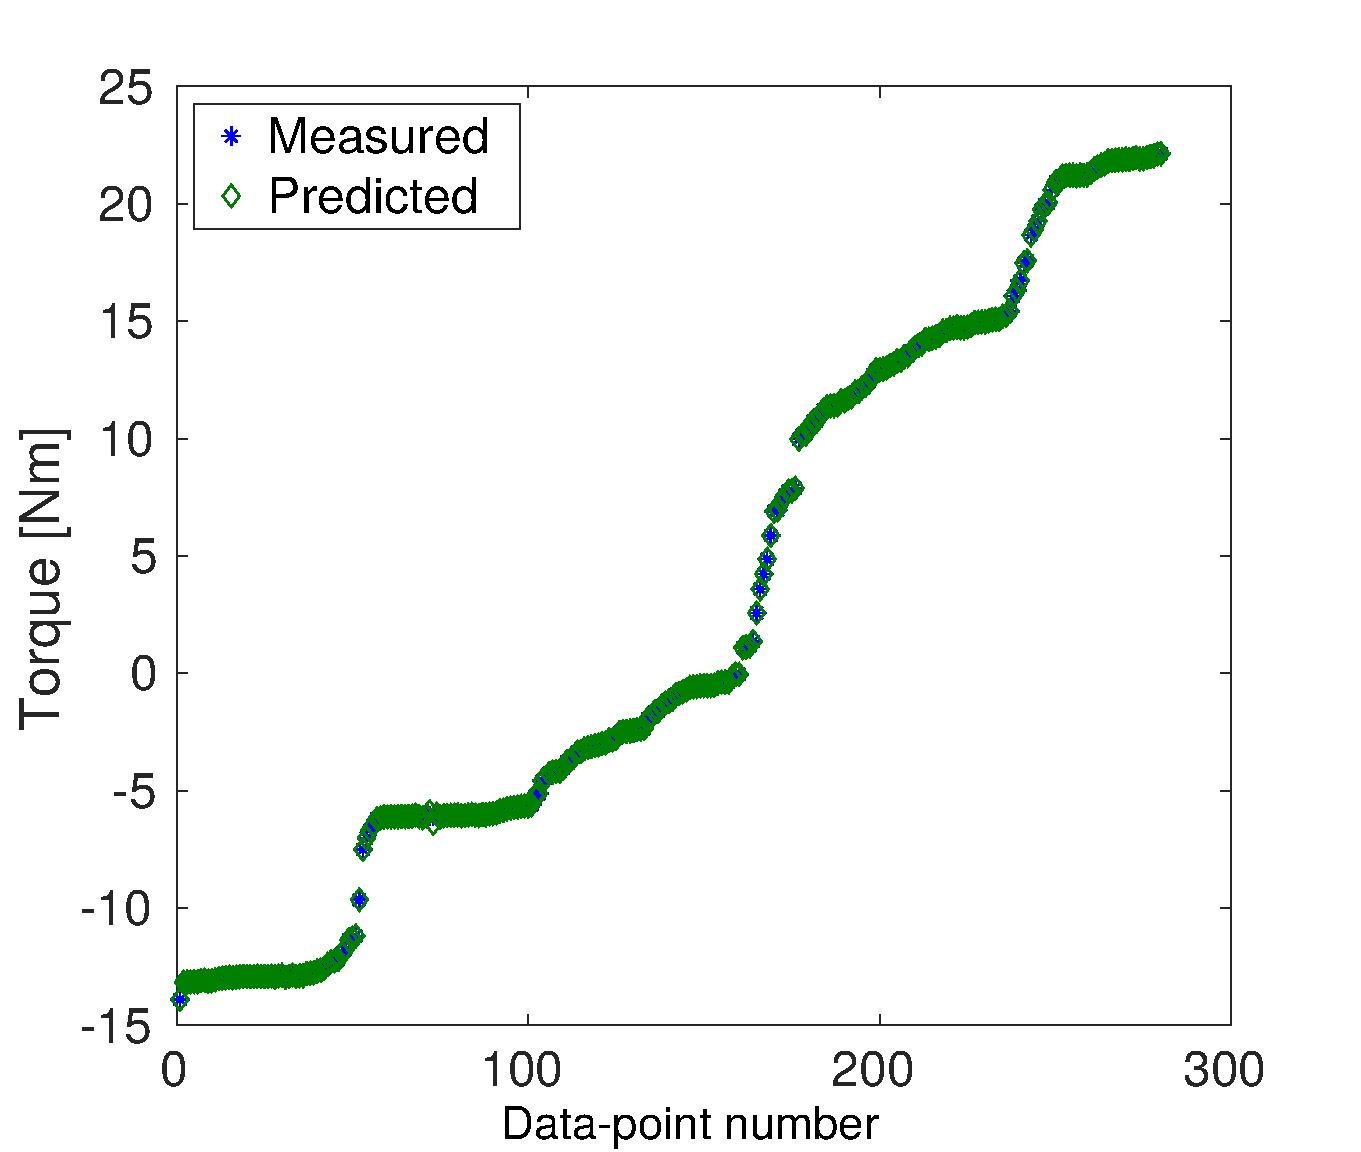
\includegraphics[width=\textwidth]{images/summer_school_study/measured_optimized_torque_A2.pdf}%
    \caption{Measured and predicted torque values of the training dataset, ordered and numbered by magnitude. The measured values (blue) and the values predicted by the Gaussian Process (green) lie on each other.}%
    \label{fig:measured_optimized_torque_A2}%
  \end{subfigure}%
  \quad
  \begin{subfigure}[t]{0.48\textwidth}%
    \centering%
    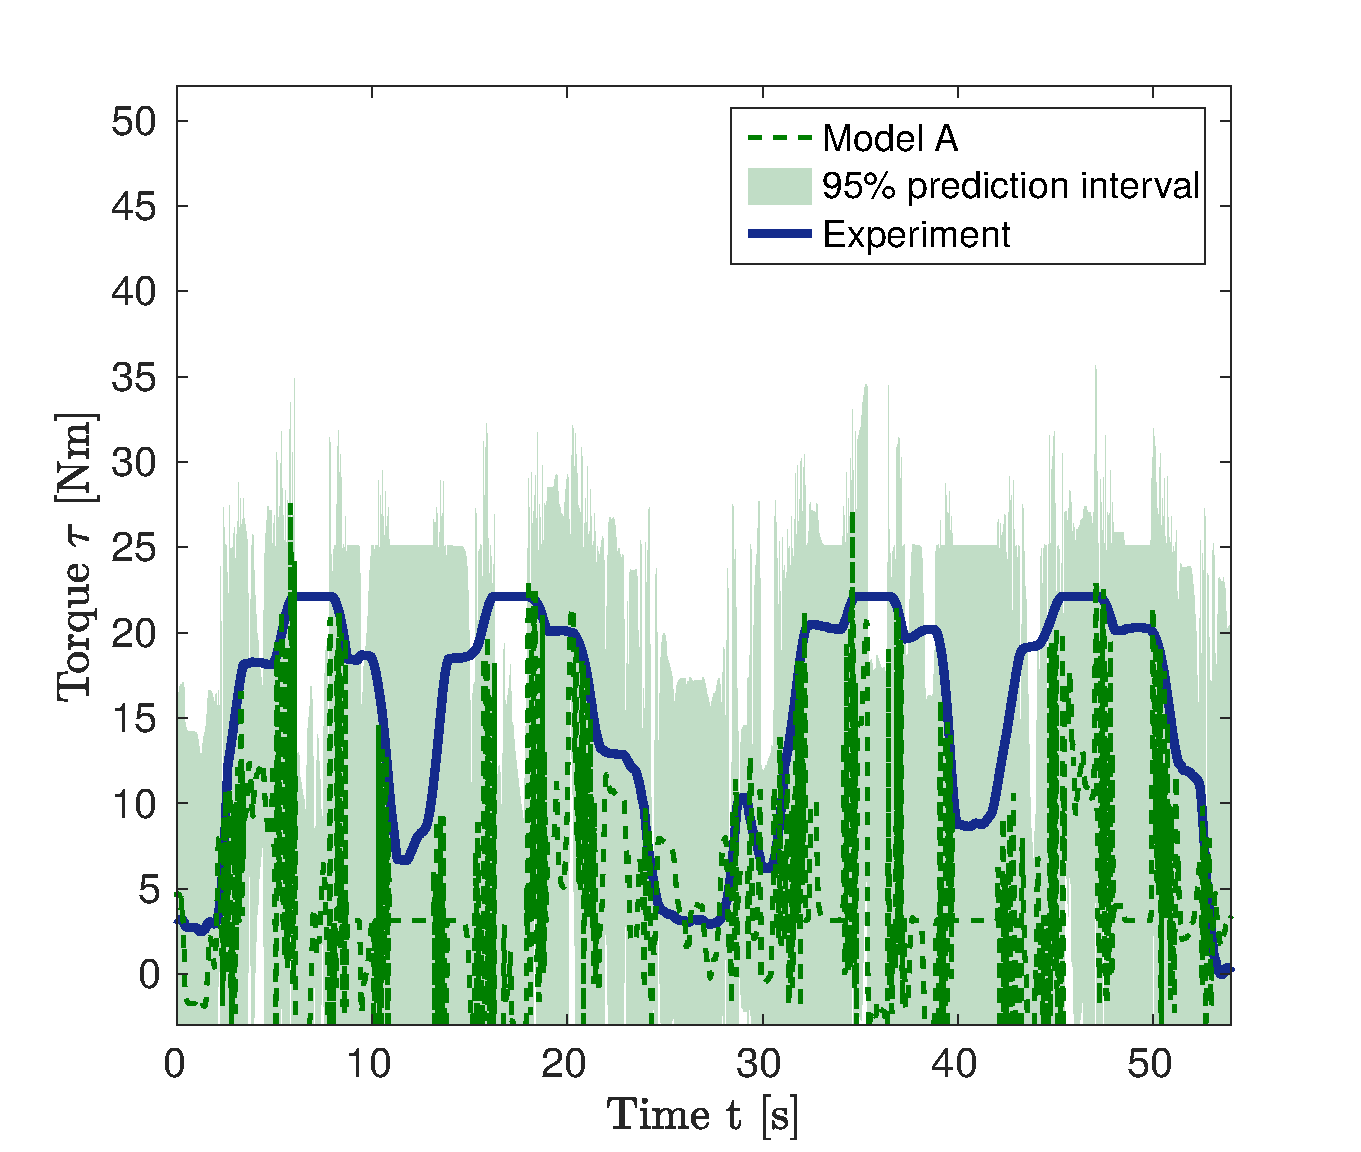
\includegraphics[width=\textwidth]{images/summer_school_study/validation_bv5_40_points_only_gamma_for_training.pdf}%
    \caption{Predicted torque values for the validation trials (green dotted line), 95\% confidence interval (light green) and the reference values of the experiment (blue). The plot reveals bad prediction capabilities of the simplified model A.}%
    \label{fig:measured_optimized_torque_A3}%
  \end{subfigure}%
  \caption{Result for the simplified model A, where, apart from the free calcium ion contractions, only the elbow angles, $\phi_e$, are used as training input instead of MTU lengths, velocities and moment arms.}
  \label{fig:measured_optimized_A2}%
\end{figure}%

\subsection{Insights of Model B}\label{ref:res_insights_b}
An advantage of model approach B is that the trained parameters are physically meaningful and allow insight into the properties of the subject specific model. Furthermore, the quality of the training data can be assessed. \Cref{fig:biceps_working_area} shows the force-length relation of the biceps muscle model using the generic and the optimized parameter values. It can be seen that the subject-specific model has a smaller slope of the force curve. 
All points of the training data set are indicated by red crosses on the curves and show the operating range of the muscle in which the model has been trained. It can be seen that the experimental training data are limited to a small range of the muscle length below its optimal CE length $l_{\CE,\text{opt}}$. In order to improve the quality of the model predictions for this subject, specific additional experimental trials can be designed for model training. They can be designed to fill in values in the missing range of operation, which in this case is for larger muscle extensions.

A low computational time of the offline parameter identification and the online evaluation of the two models would be an important measure for their practical applicability. In the present study, the training phase of Model A, i.e., optimization of the quantities for the Gaussian Process Regression using 280 training data points took \SI{2.24}{\second}. The evaluation of Model A for the validation data set containing \num{54e3} points had a duration of \SI{116}{\milli\second}.

The runtimes for model B were significantly higher. The parameter optimization lasted \SI{25}{\minute} \SI{16}{\second} and the evaluation for the validation data set had a duration of \SI{13}{\second}.

The large differences in runtime between models A and B can be explained by the inefficient implementation of the biophysical model using the MATLAB programming language. During parameter identification, this model needs to be evaluated iteratively in the optimization algorithm. In contrast, the optimization within model A works with an internal implementation of the Gaussian Process which was optimized during development of the particular MATLAB functionality.
In general, the evaluation of Gaussian Process Regression has cubic time complexity whereas, for the parameter optimization of model B, iterative solvers with linear time complexity exist.

\begin{figure}%
  \centering%
  \begin{subfigure}[t]{0.47\textwidth}%
    \centering%
    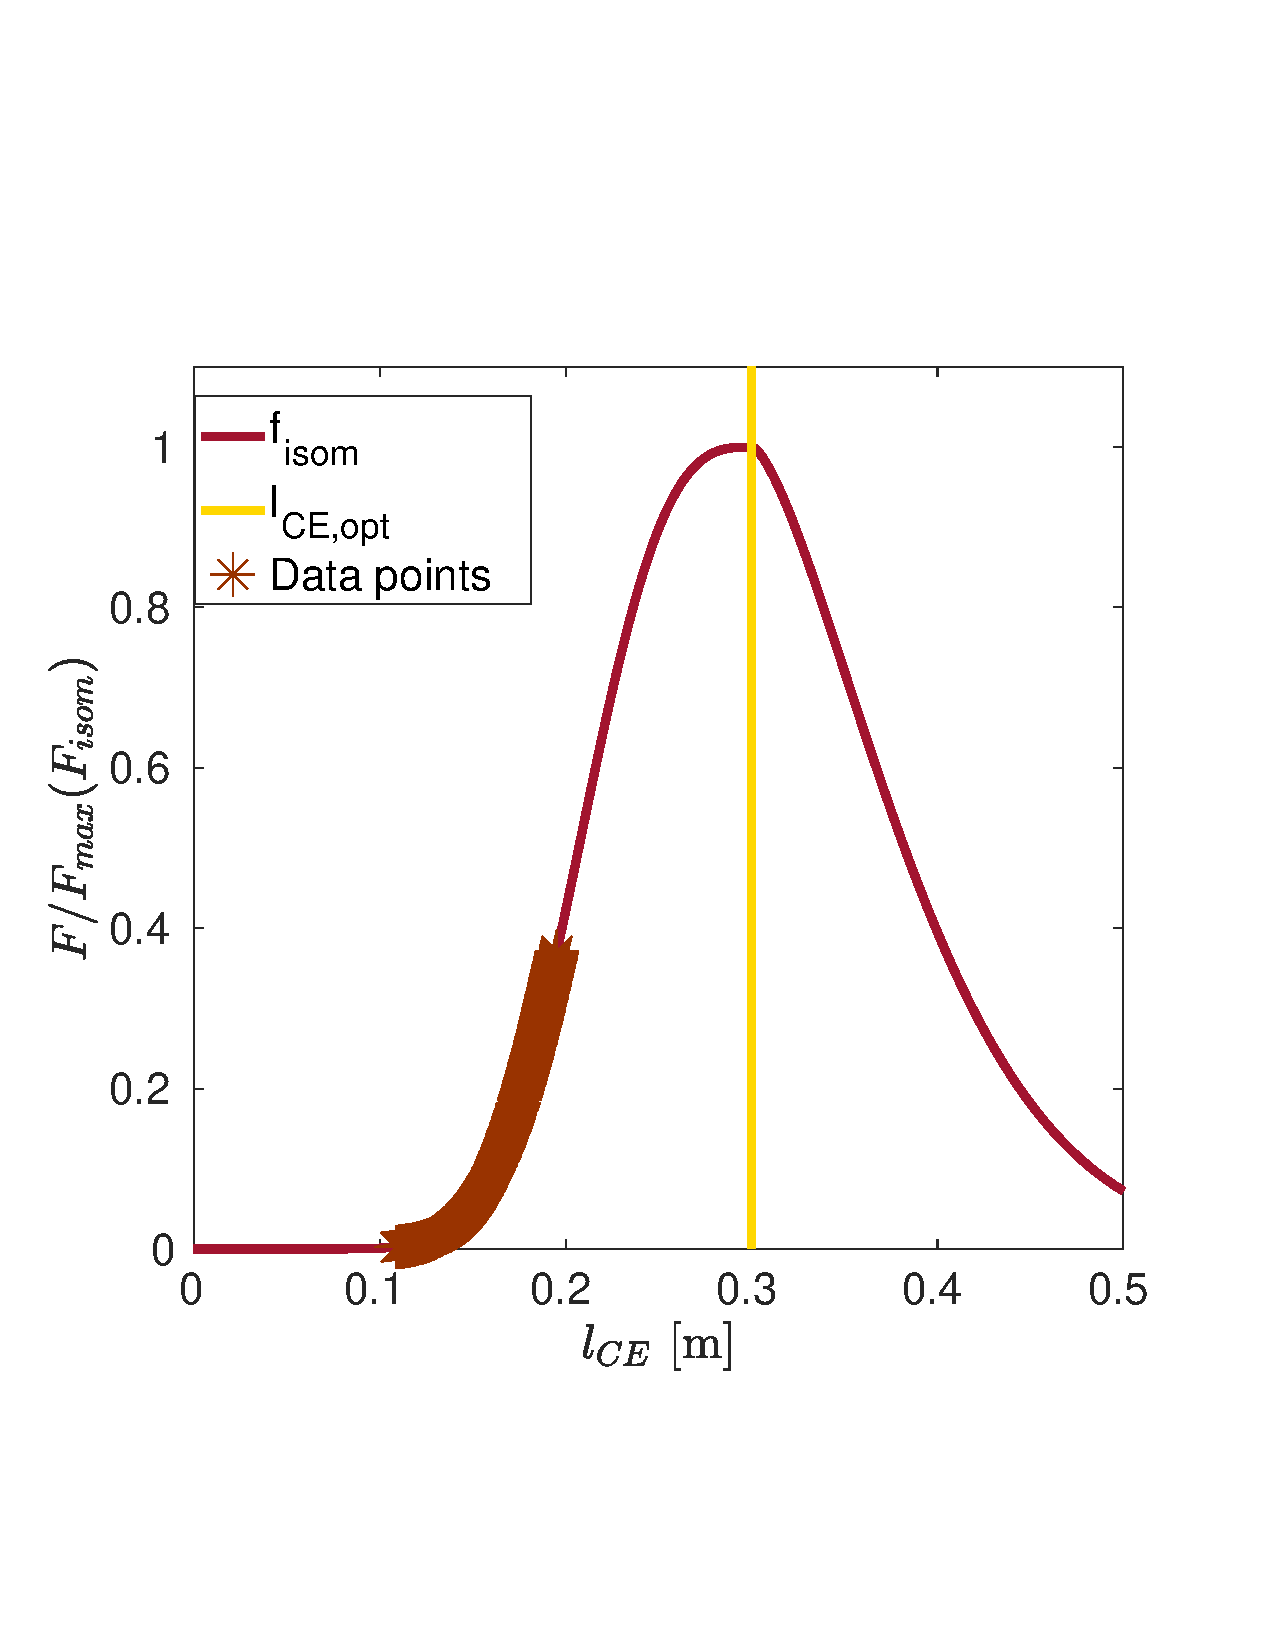
\includegraphics[width=\textwidth]{images/summer_school_study/biceps_initial.pdf}%
    \caption{Model with generic parametrization.}%
    \label{fig:biceps_a}%
  \end{subfigure}%
  \quad
  \begin{subfigure}[t]{0.47\textwidth}%
    \centering%
    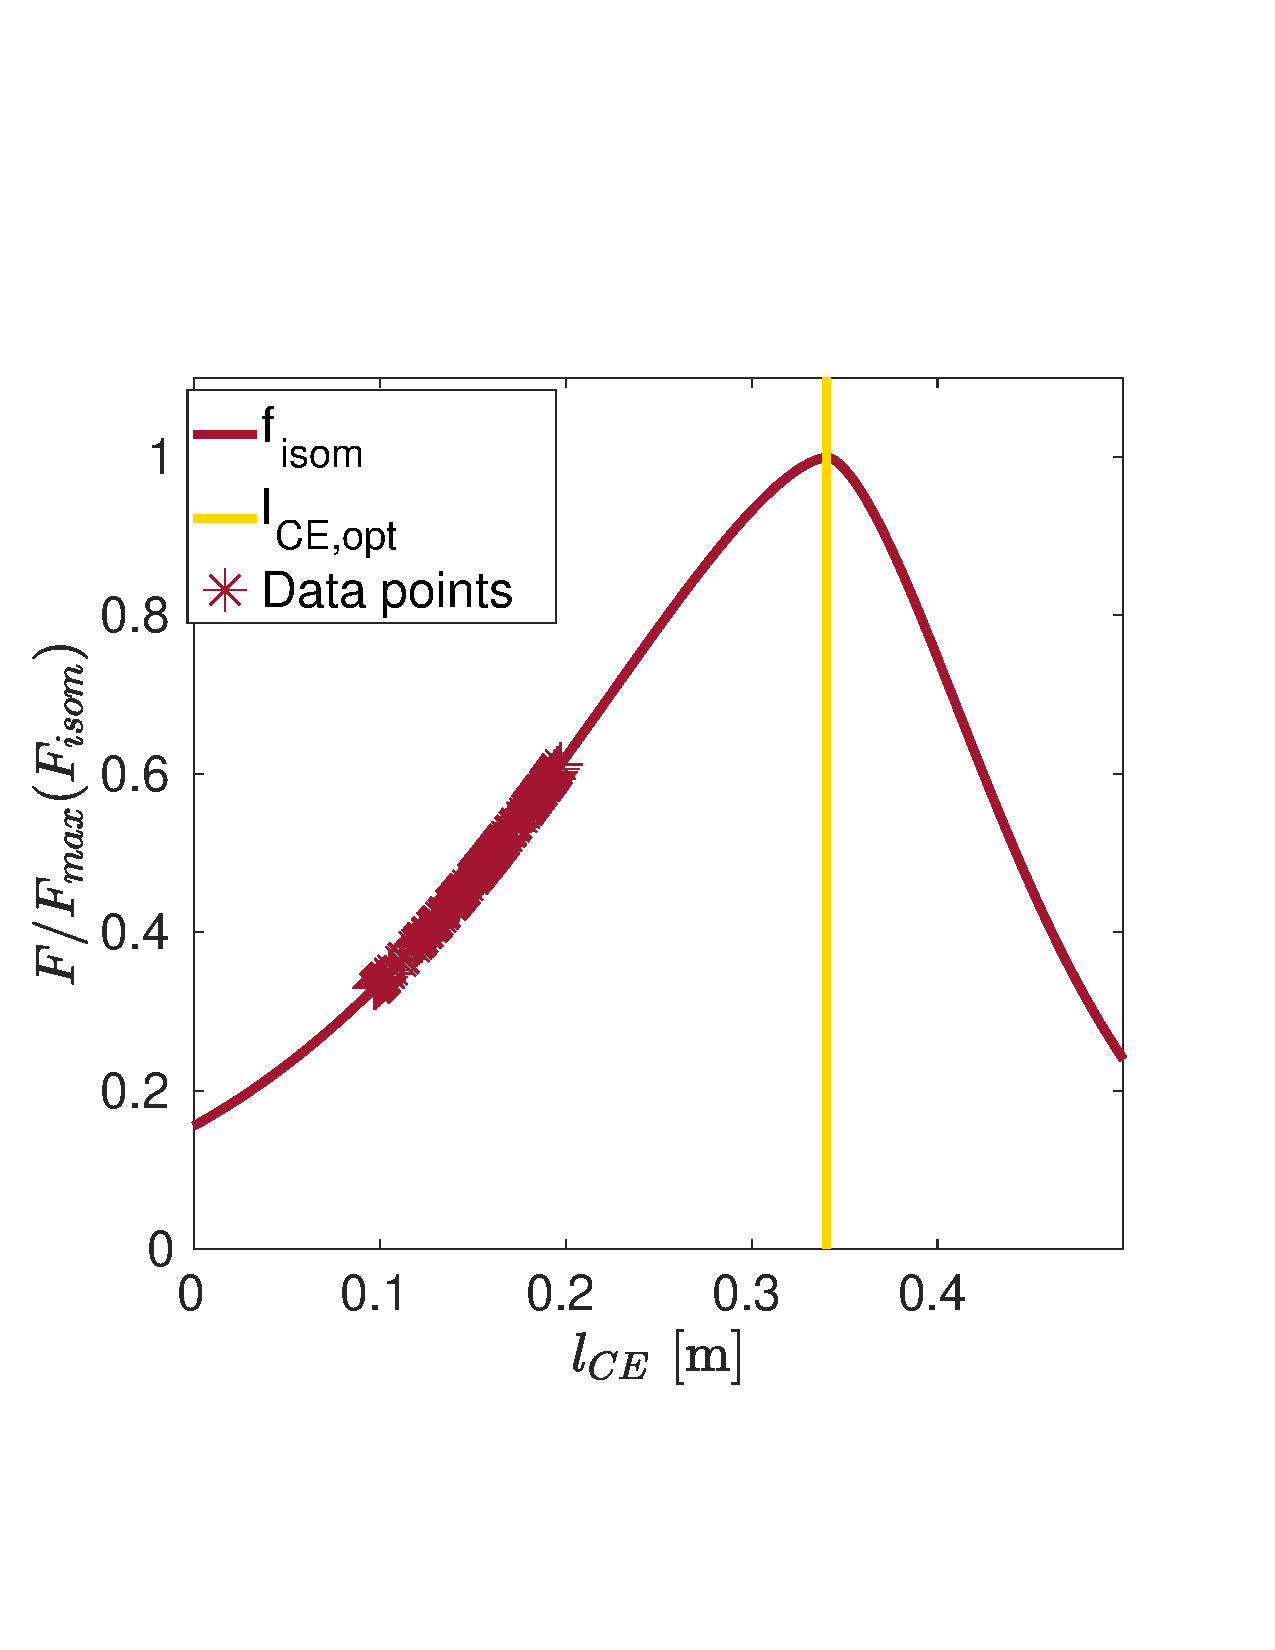
\includegraphics[width=\textwidth]{images/summer_school_study/biceps_optimized.pdf}%
    \caption{Model with subject-specific parametrization.}%
    \label{fig:biceps_b}%
  \end{subfigure}%
  \caption{Isometric force-length relation of the CE for the biceps model, analogue to \cref{fig:force_curves_generic_length}, but additionally with training data points. The points are placed on the model curve and visualize the predicted relative forces for the lengths of the CE that occurred during the training trials.}%
  \label{fig:biceps_working_area}%
\end{figure}%


\begin{figure}%
  \centering%
  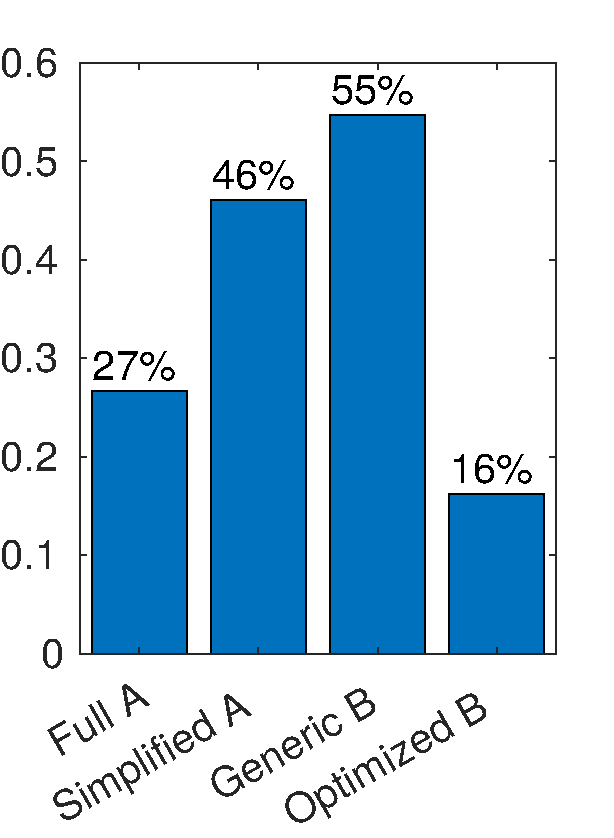
\includegraphics[width=0.35\textwidth]{images/summer_school_study/nrmse.pdf}%
  \caption{Normalized Root Mean Square errors (NRMSE) of the validation trials between the respective models and the measured values. A lower error value means a better fit.}%
  \label{fig:nrmse}%
\end{figure}%

\section{Conclusion}\label{sec:study_conclusion}
In this study, elbow torques during flexion and extension of the upper arm were predicted from motion capture data and EMG measurements. Two models, A and B, were developed. Model A is non-parametric and uses Gaussian Process Regression. Model B is biophysically informed and involves two state-of-the-art Hill-type muscle models for biceps and triceps. Experiments were conducted to generate training and validation data. These training data were used for model parameter identification. Predictions from the two models were compared to real experimental values using the validation data.

Regarding the formulation and implementation, model A requires low effort and no special knowledge about the model, except where experimental motion data is preprocessed for a specific subject. In contrast, model B needs expert knowledge about the biophysical structure and the implementation of all comprised models.

Similar holds for the offline training phase. There are no parameters in model A that have to be tuned manually, which allows a quick start. Conversely, model B requires the appropriate definition of initial values and physiological constraints for the optimization problem. However, this can also be seen as an advantage for model B, as a-priori knowledge can be integrated in such a model.

On the other hand, an advantage of model A is that additional experimental data, e.g., from neighboring muscles or additional sensors, can easily be added to the model. This is not possible with model B, where the model formulation would have to be changed.

Our studies showed that both models were able to predict the levels of torque reasonably. 
\Cref{fig:nrmse} showed the best score for model A, followed by model B. It was also seen that the generic parametrization of model B does not yield a useful prediction. The same is true for a simplified version of model A, where the elbow torque was used as training input instead of derived quantities from the motion capture system that required a complex preprocessing step.

Both models provide possibilities to assess the confidence of their predictions. With model A, confidence intervals can be computed directly from the Gaussian Processes. Their usefulness was shown in the validation where regions with large errors also had a large confidence interval. 
Model B allows insight into force-length and force-velocity characteristics of the two involved muscles. The operating ranges of the muscles during the experiments can be visualized and allow assessing whether the desired model features were covered by the training phase and, thus, will yield a good prediction.

In our study, runtimes were low for model A and high for model B in both offline and online phases. However, this is due to our prototypical implementation of model B. For larger data sizes and a more sophisticated implementation, the reverse effect is expected. The runtime complexity for the training phase is better for model B (linear in time) compared to model A (cubic in time). For the online phase, costly integration over data points is needed for model A whereas model B directly provides a differential equation of the system that can be solved efficiently. 

If EMG is used to control an exoskeleton that supports the movement of the limb, it is known that the measured signals are ahead of the intended movement by a small offset. This is a result of the time delay in the neuromusculoskeletal system. This property gives the assistive exoskeleton a short time to predict the intended movement and thereby allows a seamless integration of the artificial device with human control.

When targeted at such a real-time application, both models could be considered to be integrated into the control. Model A better fits the use case of a device that could be (re\nobreakdash-)calibrated by the patient itself. Because of the built-in estimation of prediction quality, compliance and safety could be ensured more easily even for imperfect training.
Model B would need a controlled environment such as a specialist's laboratory and careful assistance for the calibration process.
After calibration, it would promise a more natural and more responsive experience because of the subject-specific model and possibly smaller compute times.

Where real-time application is not a requirement, biophysically informed models have a high potential to leverage the understanding how the human neuromusculoskeletal system operates for given tasks.
In model B of this study, the kinematics and individual muscle dynamics were described close to the current  understanding of the system. However, several aspects where not modeled as detailed as possible. The pathway from neural stimulation to excitation and activation of the muscle, the recruitment strategies including different motor units, neural feedback loops as well as effects stemming from the 3D geometry of the muscle were not considered. Therefore, this thesis develops a more detailed, biophysically informed model including these properties in the following chapters.

The presented study reproduced what similar studies in literature have shown: Subject-specific model identification for Hill-based torque prediction models can vastly improve the prediction quality compared to generic models. Our work adds to the common knowledge that this holds also for the four-element Hill-type model that was used for model B. Furthermore, a comparison with Gaussian Process Regression was given, various advantages and disadvantages of these two approaches were identified. Future work can test the two models with more subjects and increase the variety of motion in the training experiments. For example, effects resulting from high contraction velocities or eccentric contractions could be investigated to evaluate the model's potential in more complex movements.


\chapter{Generation of Meshes for the Multiscale Models}

Multiscale models of skeletal muscles describe phenomena on different length scales and combine them into a single description. The phenomena are modeled by different sets of equations which need individual discretizations and solvers. For that, various geometrical meshes describing different physical domains are required.

The discretization considered in this work involves three-dimensional (3D) and one-dimensional (1D) meshes.
As a whole, muscles and tendons are treated as 3D domains. Muscle fascicles and myofibrils are represented by 1D fibers that are embedded in the 3D domain of the muscle.

The generation of the respective 1D and 3D meshes should be based on biomedical imaging data in order to represent actual human anatomy. The generated meshes should be of good quality such that finding numerical solutions with low error is possible. Good mesh quality usually involves mesh cells with similar lengths and angles. It should also be possible to easily partition the mesh into multiple, equally sized subdomains. This is required for efficient parallel computation.
The two requirements of good mesh quality and easy partitioning lead to the decision to employ \emph{hexahedral} elements and a \emph{structured} mesh for the 3D domains.

In this chapter, we present a workflow to construct meshes with the mentioned properties starting from biomedical data. We present novel algorithms to generate the required structured hexahedral meshes. This work contributes an implementation of the algorithms that can be used to construct all meshes needed for our biomechanical simulations.

\section{Overview and Notation of Required Meshes}\label{sec:overview_and_notation_of_required_meshes}
In the following, we summarize the meshes generated and used in this thesis and introduce their notation used in the following discussions.

The domain of the muscle belly is denoted by $\Omega_M$. A layer of fat and skin tissue is located on top of the muscle belly. It is denoted as the body domain $\Omega_B$.
The muscle belly is attached to tendons on both longitudinal ends. The tendon domains are denoted by $\Omega_{T,1}$ and $\Omega_{T,2}$. These domains are all subspaces of the 3D Euclidean space: $\Omega_M,\Omega_B,\Omega_{T,i} \subset \R^3$.

Additionally, a number $n_f$ of individual muscle fibers $\Omega_{F,i} \subset \R^3$ for $i \in \{0,\dots,n_f\}$ is introduced. Each fiber is a 1D manifold embedded in the 3D domain, i.e., $\Omega_{F,i} \subset \Omega_M$. \Cref{fig:fibers_domains} summarizes the notation of the domains.

\begin{figure}%
    \centering%
    \def\svgwidth{8cm}%
    \input{images/fiber_creation/domains.pdf_tex}%
    \caption{Visualization of the computational domains in a simulated muscle: tendons $\Omega_{T,1}, \Omega_{T,2}$, muscle belly $\Omega_M$, body domain $\Omega_B$ and fiber domains $\Omega_{F,i}$.}%
    \label{fig:fibers_domains}%
\end{figure}%

For the application of the Finite Element Method (FEM), we create meshes for each of these domains. Formally, a 3D mesh $\Omega_\text{3D}$ is given by a number of 3D elements $\{U_{\text{3D},i}\}_{i=1,\dots,n}$ with $U_{\text{3D},i} \subset \R^3$ such that their disjoint union approximates the domain,
$\dot{\bigcup}_{i=1}^{n} U_{\text{3D},i} \approx \Omega_\text{3D}$. Similar holds for 1D meshes.

The elements are non-overlapping and can be defined by nodes and edges. In the discretizations used here, no hanging nodes are allowed, i.e., at any node all adjacent elements share the node.

Furthermore, only structured, hexahedral meshes are considered in this chapter.
A 3D structured mesh is isomorphic to a 3D cartesian grid with equidistant elements. 
This has advantages for programmatically indexing nodes and elements as well as for parallel partitioning of the domain.
\Cref{fig:fiber_creation_decomposition} shows an example of a 3D structured mesh that is partitioned into twelve subdomains. The subdomains are constructed by planar cuts through the structure of the mesh. These cuts are typically defined in a way that the resulting subdomains have similar numbers of 3D elements and, thus, every process gets a similar portion of the total computational load.

The number $n$ of 3D elements is the product of the numbers $n_i, n_j$ and $n_k$ of elements in the three coordinate directions $x,y$ and $z$ of the cartesian grid,
 i.e., $n = n_i\,n_j\, n_k$.
Each element can be indexed by a triple $(i,j,k)$ of indices with the ranges $i \in \{0,\dots,n_i-1\}, j \in \{0,\dots, n_j-1\}$ and $k \in \{0,\dots,n_k-1\}$. 
In the simulation program, typically, consecutive indices $\iota$ are used that iterate over all elements $\iota \in \{0,\dots,n-1\}$ and are obtained from the index triples by the mapping 
$(i,j,k) \mapsto \iota = k\,n_i\,n_j + j\,n_i + i$.

\begin{figure}%
  \centering%
  \begin{subfigure}[t]{0.5\textwidth}%
    \centering%
    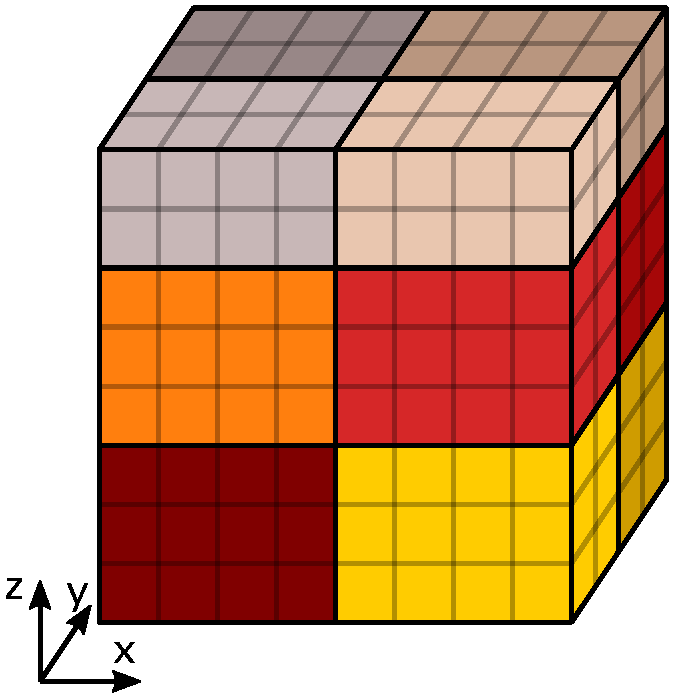
\includegraphics[width=\textwidth]{images/fiber_creation/decomposition.pdf}%
    \caption{Parallel decomposition of a 3D mesh with $n_x \times n_y \times n_z = 8 \times 4 \times 8$ elements into $2 \times 2 \times 3=12$ subdomains.}%
    \label{fig:fiber_creation_decomposition}%
  \end{subfigure}
  \quad
  \begin{subfigure}[t]{0.45\textwidth}%
    \centering%
    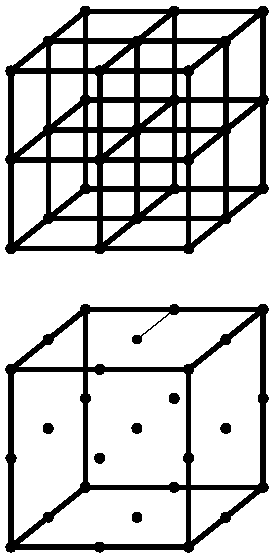
\includegraphics[width=0.6\textwidth]{images/fiber_creation/quadratic_elements.pdf}%
    \caption{Top: a linear 3D mesh with eight elements, bottom: a single quadratic element, which uses the same nodes as the linear 3D mesh at the top.}%
    \label{fig:fiber_creation_quadratic_elements}%
  \end{subfigure}    
  \caption{Structured 3D meshes that are used in the simulations: parallel partitioning and construction of quadratic elements.}%
  \label{fig:quadratic_elements_decomposition}%
\end{figure}%

The elements of such a mesh can have different numbers of \emph{degrees of freedom (dof)} depending on the desired spatial order of consistency of the Finite Element discretization. The number $n_{\text{dofs,}d\text{D}}$ of dofs in a $d$-dimensional element is computed from the number $n_{\text{dofs,1D}}$ of dofs along one coordinate direction of the element as $n_{\text{dofs,}d\text{D}} = n_{\text{dofs,1D}}^d$.
Consequently, linear elements have two dofs in 1D meshes and eight dofs in 3D meshes. Quadratic elements have three dofs in 1D and 27 dofs in 3D.

The dofs are located at the \emph{nodes} of the elements. In linear and quadratic elements, every node corresponds to a single dof. While the nodes form the \say{corners} of linear 3D elements, they are also located on the faces and in the interior of quadratic 3D elements. \Cref{fig:fiber_creation_quadratic_elements} shows a mesh with $2 \times 2 \times 2$ linear 3D elements at the top. The same 27 nodes can be used to define a single quadratic 3D element as shown at the bottom of \cref{fig:fiber_creation_quadratic_elements}. 

It is sufficient to develop a method for constructing structured 3D meshes with linear elements. 
Higher order elements can be geometrically constructed by using the nodes of multiple adjacent linear elements.
To generate both linear and quadratic elements, we always begin with generating a mesh with even numbers $n_i,n_j$ and $n_k$ of elements in the coordinate directions. Then, linear and quadratic meshes can be extracted from the set of nodes. Similarly, a linear 1D mesh with an even $n_i$ can be easily converted into a quadratic 1D mesh.

The next sections describe workflows and algorithms to construct 3D meshes for the domains $\Omega_M,\Omega_B,\Omega_{T,i}$ and 1D meshes for the fibers $\Omega_{F,i}$ based on anatomical information. \Cref{sec:fiber_meshes_related_works} gives an overview over available meshing software tools and existing algorithms in literature. Then, \cref{sec:preprocessing_of_the_muscle_geometry} presents a workflow to extract a smooth surface representation from anatomical imaging data. In \cref{sec:ser_alg_meshes}, two serial algorithms are presented to generate 3D meshes and 1D fibers meshes. The next section, \cref{sec:parallel_algorithm}, extends these serial algorithms formulating a parallel algorithm and shows and discusses results. Finally, \cref{sec:meshes_summary_and_conclusion} gives a summary and concludes this chapter.

\section{Related Work}\label{sec:fiber_meshes_related_works}

Generating volumetric meshes for domains enclosed by a given surface is a task that is frequently needed in computational science. It is a preprocessing step whenever spatially discretized models have to be solved numerically. In consequence, a vast amount of literature has addressed this algorithmic task and various approaches and methods have been proposed. Moreover, numerous software packages that solve this problem exist. Especially tools for Computer Aided Design and Engineering (CAD/CAE) as well as free and commercial preprocessing tools and Finite Element solver software include functionality to generate meshes from given surfaces.

An example from the biomechanical domain is \cite{untaroiu2013finite}. The study develops a Finite Element model of the lower limb of an occupant of a car with the aim to investigate injury scenarios during traffic crashes.
The lower extremity geometry was obtained by computer tomography (CT) and magnetic resonance imaging (MRI) scan data of a 50th percentile male volunteer. Different meshes of bones and ligaments were created using the three tools IA-FEMesh \cite{grosland2009ia}, TrueGrid \cite{TrueGrid} and Hyper-Mesh \cite{Hypermesh} which will be outlined in the following.

\emph{IA-FEMesh} (University of Iowa, Iowa City, USA) is an open source tool to generate hexahedral meshes \cite{grosland2009ia}. It provides an interactive environment where existing geometries can be loaded. In a visualization window, bounding boxes, called blocks, can be positioned such that they contain the whole geometry. A structured grid on the block is then projected onto the surface of the geometry. Multiple blocks can be placed to account for more complex geometries. The resulting surface mesh is improved using Laplacian smoothing which equalizes the edge lengths of the elements.
The interior nodes are generated using interpolation.
The result is a structured mesh if only one block is used or an unstructured mesh if multiple blocks are used. Further operations to manage mesh density, visually manipulate the meshes and add material properties, load and boundary conditions are available. The model can be exported in a file format for Finite Element analysis with ABAQUS (Dassault Systèmes, Vélizy-Villacoublay, France) \cite{ABAQUS}.

The second tool is \emph{TrueGrid} (XYZScientific Applications, Livermore, USA) \cite{TrueGrid}. It is a commercial toolkit to generate hexahedral meshes. The project was started in the early 1990s as the successor to the even older preprocessor software \emph{INGRID}. Similar to \emph{IA-FEMesh}, a projection method and a multi-block technique are used. Some effort has been put into dealing with holes and sewing together dissimilar blocks.

The third tool is \emph{Hyper-Mesh}, the commercial pre- and postprocessing toolkit of Hyperworks (Altair HyperWorks, Troy, USA) \cite{Hypermesh}.
Altair sells infrastructure and solvers for a multitude of physics and is targeted at a wide range of industries. 
Being a commercial vendor, information about the internals of their preprocessing software are hardly provided.

More meshing software exists, such as CGALmesh \cite{Jamin2015CGALmesh} for tetrahedral meshes. The package gives quality guarantees of their generated meshes and includes four mesh optimization algorithms to further improve the mesh quality.

Another application-oriented work dedicated to the use of commercial tools is \cite{Ellankavi2018}. A workflow for patient-specific modeling, simulation and analysis of the interaction between a residual lower limb stump and the socket of a prosthesis is presented. Imaging data were taken from magnetic resonance diffusion tensor imaging where also the preferred diffusion direction of water molecules along muscle fibers is captured. The open source tool MedInria (National Institute for Research in Digital Science and Technology (Inria), France) \cite{vichot2012cardiac} was used to extract muscle fibers. The residual limb data were processed using the commercial 3D image segmentation software Simpleware ScanIP (Synopsys, Mountain View, USA). Auxiliary tasks were performed using MATLAB (MathWorks,	Natick, USA) scripts. The commercial multiphysics solver LS-DYNA (LSTC/Ansys, Canonsburg, USA) was used for the simulations.

Commercial tools usually have the advantage that more development effort was put into them, than is possible for open source codes from the scientific community. This often leads to more robust and user-friendly software. An advantage of open source software is that the used algorithms are disclosed to everyone. They are often well documented or described in a publication. This allows to assess the expected quality of the generated meshes. Conversely, commercial vendors usually have no interest in revealing their internal algorithms.

For our simulation, structured, hexahedral meshes are needed. Several of the described tools are able to generate hexahedral meshes, however the meshes are typically unstructured. For our special need of 1D muscle fibers embedded in a 3D mesh, we develop our own method that is based on the ideas of existing algorithms. In the following, an overview over the algorithmic common knowledge of creating simplex meshes and hexahedral meshes is given as a basis.

% other 3D meshing
% tets
Triangulating a 2D domain is the archetype of mesh creation. The triangulation named after B. Delaunay was formulated in 1934 \cite{delaunay1934sphere}. For a given set of points, it maximizes the minimum angle of the triangles and, thus, avoids small angles. Therefore, a guarantee on the quality of the triangulation is given.

In 1995, J. Ruppert presented the Delaunay refinement algorithm \cite{Ruppert1995}, which constructs a Delaunay triangulation conforming to prescribed connected points. This algorithm is still commonly used and also part of numerous derived meshing techniques.

In 1997, P. Chew developed an algorithm for meshing a 3D domain with tetrahedra \cite{chew1997guaranteed} and proved that the aspect ratio of the tetrahedra is bounded, i.e., degenerate, \say{flat} tetrahedra, called slivers, are avoided.

The authors of \cite{Alliez2005Variational} propose a variational approach to triangulation where a quadratic energy function is minimized. During minimization both vertex positions and connectivity are optimized. This leads to better quality meshes than by simple Delaunay triangulations.

% tets to quads:
Hexahedral meshes can be obtained from certain tetrahedral meshes by splitting up each tetrahedron into four hexahedra. This is discussed in \cite{eppstein1999linear}. A remaining issue is that the generated meshes from this procedure are highly unstructured and some hexahedra have poor quality, whereas the goal would be to construct elements that are almost equilateral.

% hexs
A different approach is to directly generate a hexahedral mesh for the given surface geometry.
The survey in \cite{owen1998survey} identifies four different strategies for generating unstructured hexahedral meshes.

The first one is a \emph{grid-based} approach. It was introduced in \cite{schneiders1996grid,schneiders1997algorithm}. The interior of a given solid is filled with a regular and cartesian grid of as many hexahedral elements as fit into the space. Then, the gaps at the surface are filled with additional elements. This method is robust but can lead to poor quality elements near the surface. 
%The orientation of the interior grid highly depends on the orientation of the initial surfaces and may not be the natural orientation of the given volume.

The second approach for generation of hexahedral meshes are \emph{medial surface methods} \cite{price1995hexahedral, price1997hexahedral}. First, the volume is decomposed into subregions by medial surfaces such that the resulting domains are one of only 13 possible types. Predefined templates are used to fill the domains with hexahedral elements. Then, the continuity between the domains is ensured using linear programming. This approach gives good results for some geometries but has robustness issues when general geometries are considered.

The third approach is called \emph{plastering}. It was first described by \cite{blacker1993seams} and continued by \cite{staten2006unconstrained,staten2010unconstrained}.
It is a moving-front method where hexahedral elements are placed in layers starting at the boundary and moving towards the interior. Intersection of faces has to be detected when the fronts meet in the interior and rules for connecting to existing faces have to be defined.
During this process, complex shaped voids can occur in the interior. When it is no longer possible to fill the voids with hexahedra already placed elements have to be removed.
A new method, called unconstrained plastering, starts from an unmeshed volume boundary. The approach has general robustness issues and is not guaranteed to find a solution for arbitrary boundaries.

The forth approach is \emph{whisker weaving}, introduced by \cite{tautges1996whisker} and extended by \cite{ledoux2008extension,kawamura2008strategy}. Here, the dual of the hexahedral mesh is considered. The dual consists of the three surfaces per hexahedron that lie in the planes of symmetry. The surfaces of all hexahedra form topological loops. 
The principle is now to first construct the dual of the mesh, which can be determined from the given boundary surface. Then, the actual hexahedral mesh is created from the dual, using the surfaces as guides where to place the elements.
The dual forms topological loops inside the volume. One important criterion for generating good quality meshes is that self-intersections of these loops are resolved in a first step.
The approach, used with subsequent smoothing, can produce meshes of good quality. However, no guarantee is given. One problem is that the resulting mesh depends on the quality of the surface mesh and that the number of nodes can increase significantly during the method.

For the whisker weaving method and for some plastering methods, a quadrilateral mesh of the surface is required. Algorithms for creating high quality quadrangulations of closed surfaces exist \cite{dong2005quadrangulating,Kovacs2011Anisotropic,Bessmeltsev2012,Meng2016Consistent}.

Other approaches start with 3D volumetric medical imaging data instead of surfaces. In \cite{Zhang2003,Zhang20053DFiniteElementMeshing}, adaptive tetrahedral and hexahedral meshes are created from volumetric data using octree subdivision. The method avoids hanging nodes and allows a feature sensitive adaptivity. While adaptive meshing methods can reduce the number of elements in the interior of the volume, a problem is that the worst quality elements are generated at the boundary, the location where the solution in a Finite Element study usually is most interesting.

\nocite{Gregson2011}

Multiple reasons make the previously outlined approaches unsuited regarding the needs for our parallel muscle simulation. 

(i) The generated meshes are unstructured. When performing domain decomposition for parallel computing on unstructured meshes, graph-partitioning methods have to be used. Storing an unstructured mesh requires storage of element adjacency information. Partitioned meshes additionally require storage of the adjacent processes. In contrast, structured meshes can be trivially decomposed and stored efficiently. A decomposition can be represented in memory by a very low number of parameters.

(ii) The presented methods are designed for hexahedral meshing of arbitrary volumes. Robustness and mesh quality at the same time remain issues that are not completely solved for most of the algorithms. Often, expensive smoothing steps are needed to increase mesh quality.

(iii) In general, either no assumption can be made about orientation or alignment of hexahedra in the interior, or, for the grid-based approach, the elements at the surface have poor quality. Having a mesh that is consistently aligned with, e.g., the main diffusion direction or the preferential direction of the anisotropic material or the muscle fibers can reduce numerical errors in the Finite Element solution.

Consequently, a more scenario specific solution is needed that can avoid the mentioned issues. Such solutions can also be found in the literature. An example is \cite{blemker2005three}, where 3D Finite Element models for various complex muscle geometries around the hip are generated from magnetic resonance images. Segmentation and surface mesh generation are performed using the old, unmaintained software \emph{Nuages} (Inria, France) \cite{Nuages}.
Then, a 3D hexahendral mesh is generated using TrueGrid. A structured template mesh on a unit square is mapped to the horizontal slices of the muscle geometry that resulted from the segmentation. After mesh smoothing, the slices are connected vertically to form a 3D mesh. 
Fiber directions are described by Bezier curves in a reference volume and mapped to the muscle geometry using the same mapping. The fiber direction then are used in a transversely-isotropic material formulation. Simulations are performed using the Finite Element solver \emph{Nike3D} (Lawrence Livermore National Lab, Livermore, USA) \cite{Nike3D}.

We base our work on this study and use a similar mapping from a template mesh to the actual muscle volume. In comparison to \cite{blemker2005three}, we use an improved mapping based on harmonic maps, which potentially leads to better quality meshes on the slices of the muscle. Instead of the unit circle template mesh, we experiment with different reference meshes and evaluate their quality.

In the study of \cite{blemker2005three}, fiber directions are defined based on anatomically assumed directions.
However, the definition is carried out on the cuboid reference geometry. This means that the authors mentally morph the muscle geometry into the reference geometry in order to define fiber directions, using their expertise. Then, the fiber directions together with the cuboid are transformed back to the actual geometry. This approach simplifies the definition of the fibers. However, defining the fiber direction directly on the muscle geometry can lead to better results. Thus, our approach is to automatically estimate fiber directions and define fibers directly in the muscle domain. At the same time, the 3D mesh and 1D fibers are aligned in our work to allow for better numerical and data structure properties of the discretization. 

The definition of fiber directions follows a method proposed in \cite{Choi2013}. 
The directions are assumed to follow a divergence free vector field. Such a field can be created by taking the gradient of the solution of the Laplace equation. Neumann boundary conditions are defined at the attachment points of the muscle tendon complex. The solution of the Laplace equation corresponds to the pressure values of a potential flow. Its gradient corresponds to the velocity and individual fascicles or fibers can be obtain by tracing streamlines through the velocity field.
This approach is extended and validated by the studies in \cite{Inouye2015} and \cite{Handsfield2017}. We incorporate this method into our workflow.

\section{Preprocessing of the Muscle Geometry}\label{sec:preprocessing_of_the_muscle_geometry}

The first step towards creating a structured mesh is to obtain a representation of the surface of the muscle. 
Starting point is a human biomedical imaging data set. In this section, two possible workflows are presented how to extract the muscle and tendon surfaces from imaging data. 
The two workflows are visualized in \cref{fig:scheme_preprocessing}. The workflow using the branch on the left side in \cref{fig:scheme_preprocessing} is automized but only works for the particular data set and extracting the biceps muscle.
The right branch involves manual steps and is applicable for any muscle geometry.

% overview over subsections

\begin{figure}%
  \centering%
  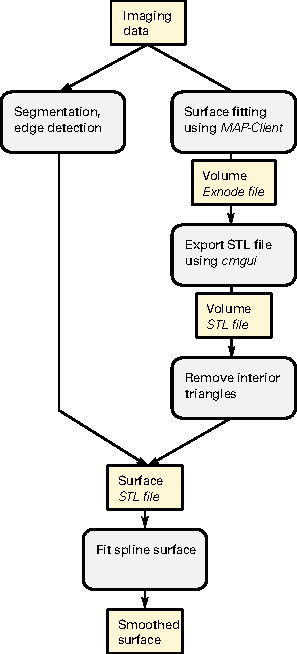
\includegraphics[height=15cm]{images/fiber_creation/scheme_preprocessing.pdf}%
  \caption{Workflow of generating a surface representation of the muscle and tendons from imaging data. Operations and intermediate results are shown as gray and yellow boxes, respectively. Two alternatives are given by the two branches. On the left, the imaging data are automatically processed to directly retrieve points on the surface of the muscle. The right branch achieves the same with three steps of which the first one involves manual adjustments. At the end, a spline surface smooths the collected data from both possibilities to yield the resulting surface representation.}%
  \label{fig:scheme_preprocessing}%
\end{figure}%

\subsection{Data Source}
Anatomic images provide the basis for the extraction of muscle geometries.
Our used data set originates from the Visible Human Project \cite{visible_human_male} of 
the United States National Library of Medicine. 
The project has published anatomic images derived from a male corps, among other data sets.
The data, known as \say{Visible Human Male}, were published in 1994.
Colored images of transversal cross sections were obtained by cryosectioning.
A total of \num{1871} images with dimensions of \num{2048} by \num{1216} pixels and 24 bit color depth visualize the whole human body. Parts of the upper arms are contained in approximately 500 of these images. The size of a pixel is \SI{0.33}{\milli\meter} in transversal direction and \SI{1}{\milli\meter} in axial direction. The size of the complete set of JPEG compressed images is \SI{772}{\mega\byte}. Cropping and selecting the relevant portions of the upper arm extracts a dataset with the size of \SI{35}{\mega\byte}.

An extract of an image of the upper arm is given in \cref{fig:vhp_image}. 
The location of biceps and triceps brachii muscles can be identified in the dark red tissue. For the biceps, the two muscle heads are visible, separated by the bright diagonal line from bottom left to top right. For the triceps, at least two of the three heads can be identified. The blue background is colored frozen gelatin that was needed during cryosection to stabilize the arms.

\begin{figure}%
  \centering%
  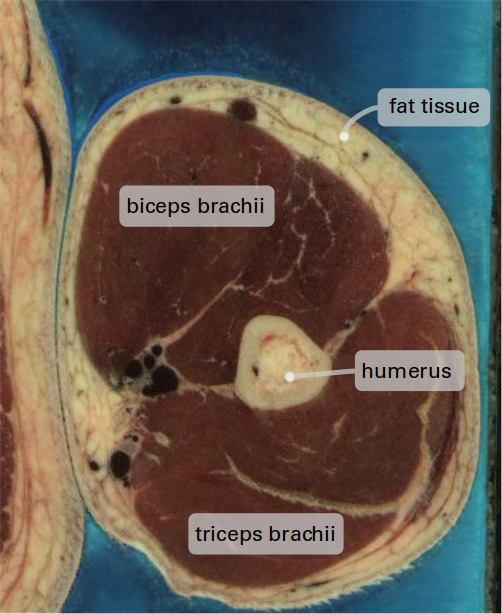
\includegraphics[height=10cm]{images/fiber_creation/vhp.png}% 0483
  \caption{Exemplary extract of image number 483 from the Visible Human Male. A transversal slice of the left upper arm is shown as seen from the bottom. The biceps and triceps muscles as well as the humerus bone can be identified. }%
  \label{fig:vhp_image}%
\end{figure}%

\subsection{Automatic Surface Extraction}
This section outlines the automatic algorithm to obtain the muscle surface from the Visible Human Male data set. The scheme corresponds to the left branch in \cref{fig:scheme_preprocessing}. The algorithm was implemented in a Python script as part of the Bachelor thesis of Kusterer \cite{Kusterer} that was supervised by me.
The algorithm is capable of extracting muscle and bone geometries from the mentioned imaging dataset.

At first, the color values in the images are used to segment the pixels into muscle tissue, surrounding tissue and skeletal structure. The algorithm traverses the selected and cropped relevant parts of the images. 
%For example, to consider the biceps muscle, the image region of pixels coordinates $(x,y)$ with $x \in [1300,1720] $ and $ y\in[1030,1720]$ are considered in the images with numbers 284 to 778. 

For every such part of an image, pixels that match a certain range in the RGB color space are marked and categorized. The categories are muscle tissue and, for demonstration, also bone tissue. The corresponding color ranges are given in \cref{tab:color_ranges}.

The color based classification does not succeed everywhere as the white shade corresponds not only to bone material but also to fat and other tissue. Therefore, the algorithm removes artifacts located near the outer gelatine from the set of pixels that was categorized as bone. 

\begin{table}
  \centering%
  \begin{tabular}{|l|lll|}
    \hline
    & red & green & blue\\
    \hline
    muscle & $60 - 100$& $30-75$   & $15-60$\\
    bone   & $145-255$ & 1$35-205$ & $60-160$\\
    \hline
  \end{tabular}
  \caption{Ranges in the RGB color space to identify pixels of muscle and bone segments. The numbers correspond to 24 bit colors with the range $[0,255]$ for every color channel.}%
  \label{tab:color_ranges}%
\end{table}

Exemplary results for image number 483 are given in the left column of \cref{fig:extraction}.
It can be seen that the marked regions for muscle and bone have gaps in the interior resulting from differently colored tissue inside muscles and bones. On some images, the set of pixels also includes small objects outside the actual muscle and bone regions.

To reduce the gaps and small objects, the morphological operations \emph{closing} and \emph{opening} are applied on the data. These operations consist of \emph{dilation} and \emph{erosion} steps. Both are pixel based operations that traverse the dataset and for every pixel consider a window of $3\times 3$ pixels centered at the current position. Dilation picks the maximum value and erosion the minimum value from this window and assigns it as the pixel's value in a new image. In our case, values of zero and one correspond to non-categorized and categorized pixels, respectively.

Closing consists of dilation followed by erosion and closes small gaps or holes in the marked objects. Opening consists of erosion followed by dilation and removes small artifacts outside the actual bone and muscle areas. It was found effective to perform both dilation and erosion twice in sequence to yield good results containing almost no more holes nor unwanted small objects.

Next, the algorithm determines the contours of all regions with marked pixels. This leads to lines with a width of one pixel that enclose the muscle and bone areas. The right column of \cref{fig:extraction} shows the results after this step. It can be seen that numerous gaps have been closed by the morphological operations. In some images, as in the considered example, the muscle area gets split into multiple smaller enclosed regions, which is not desired. These images skipped in the processing. However, proper contours of the biceps are found in the majority of images. 

\fboxsep=0mm   % padding thickness
\fboxrule=1pt   % border thickness
\begin{figure}%
  \centering%
  \fcolorbox{black}{black}{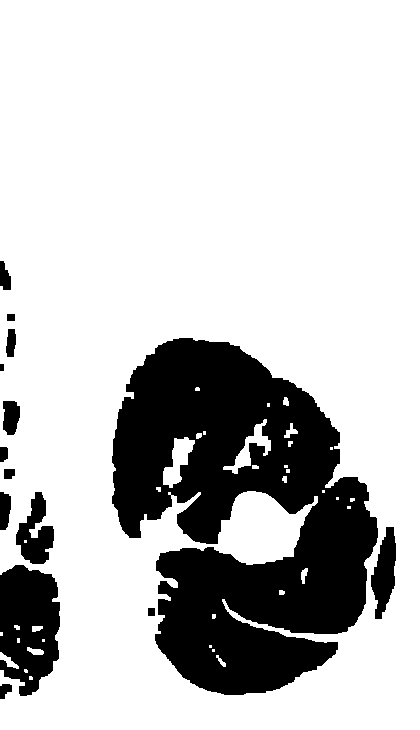
\includegraphics[height=7cm,trim=0 0 0 6cm, clip]{images/fiber_creation/extraction_segmentation_482.png}}\quad%
  \fcolorbox{black}{black}{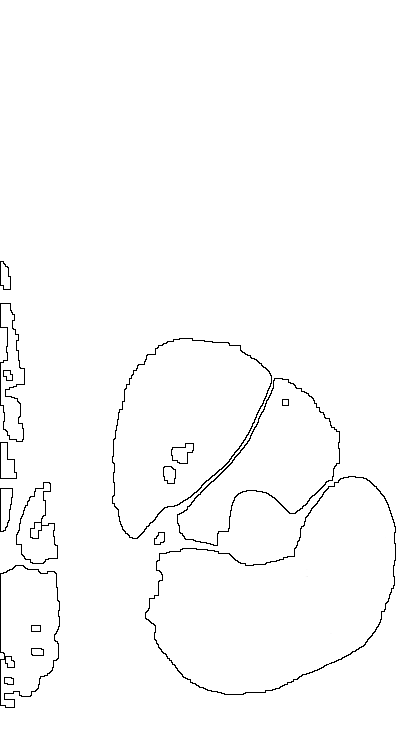
\includegraphics[height=7cm,trim=0 0 0 4cm, clip]{images/fiber_creation/extraction_contour_482.png}}\vspace*{5mm}\\
  \fcolorbox{black}{black}{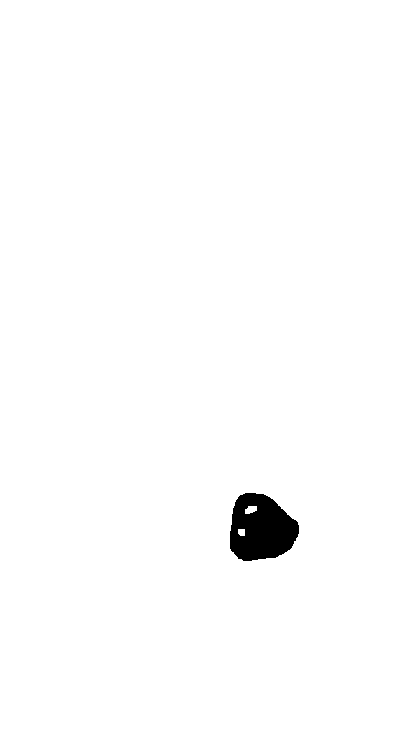
\includegraphics[height=7cm,trim=0 0 0 6cm, clip]{images/fiber_creation/extraction_bone482.png}}\quad%
  \fcolorbox{black}{black}{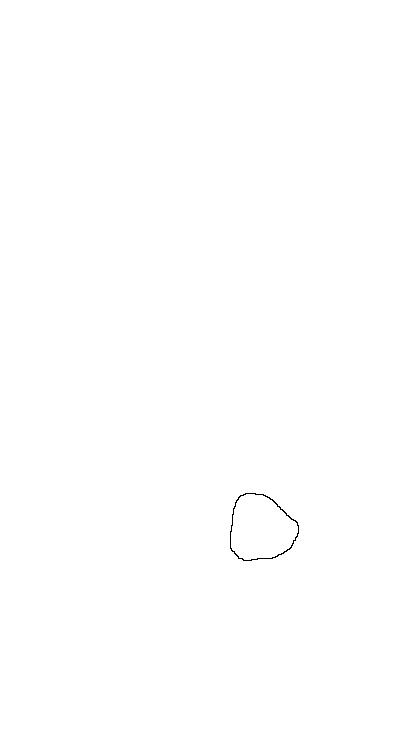
\includegraphics[height=7cm,trim=0 0 0 6cm, clip]{images/fiber_creation/extraction_surface_bone482.png}}%
  \caption{Intermediate steps of the algorithm to determine surface geometry of muscles and bones. The left columns shows pixels from the image in \cref{fig:vhp_image} that were categorized to be muscle tissue (top) and bone material (bottom). The right column shows a later step in the algorithm, where the surface of muscle (top) and bone (bottom) is estimated.}%
  \label{fig:extraction}%
\end{figure}%

In the next step, a single contour for each of muscle and bone is obtained in every image. If there are multiple contours per image, the one that is located closest to the upper right corner of the image is selected for the muscle. If all contours in an image are shorter than 20 pixels, this is an indication for bad segmentation quality and the whole image gets discarded. Because of the discarded images the resulting surface description has a lower resolution at the respective locations. This is not a problem as the data is subsequently approximated by a smooth spline surface.

The result is a set of contours for muscle and bone in the cross-sectional planes of the images. Combining these, we get a point cloud in 3D space that approximates the surface of the biceps muscle and the surfaces of the considered bones humerus, ulna and radius. Using these points, a spline surface can be fitted and subsequently triangulated. Resulting surfaces for the biceps and humerus bones are shown in \cref{fig:extraction_result}.
%
\begin{figure}%
  \centering%
  \begin{subfigure}[t]{0.48\textwidth}%
    \centering%
    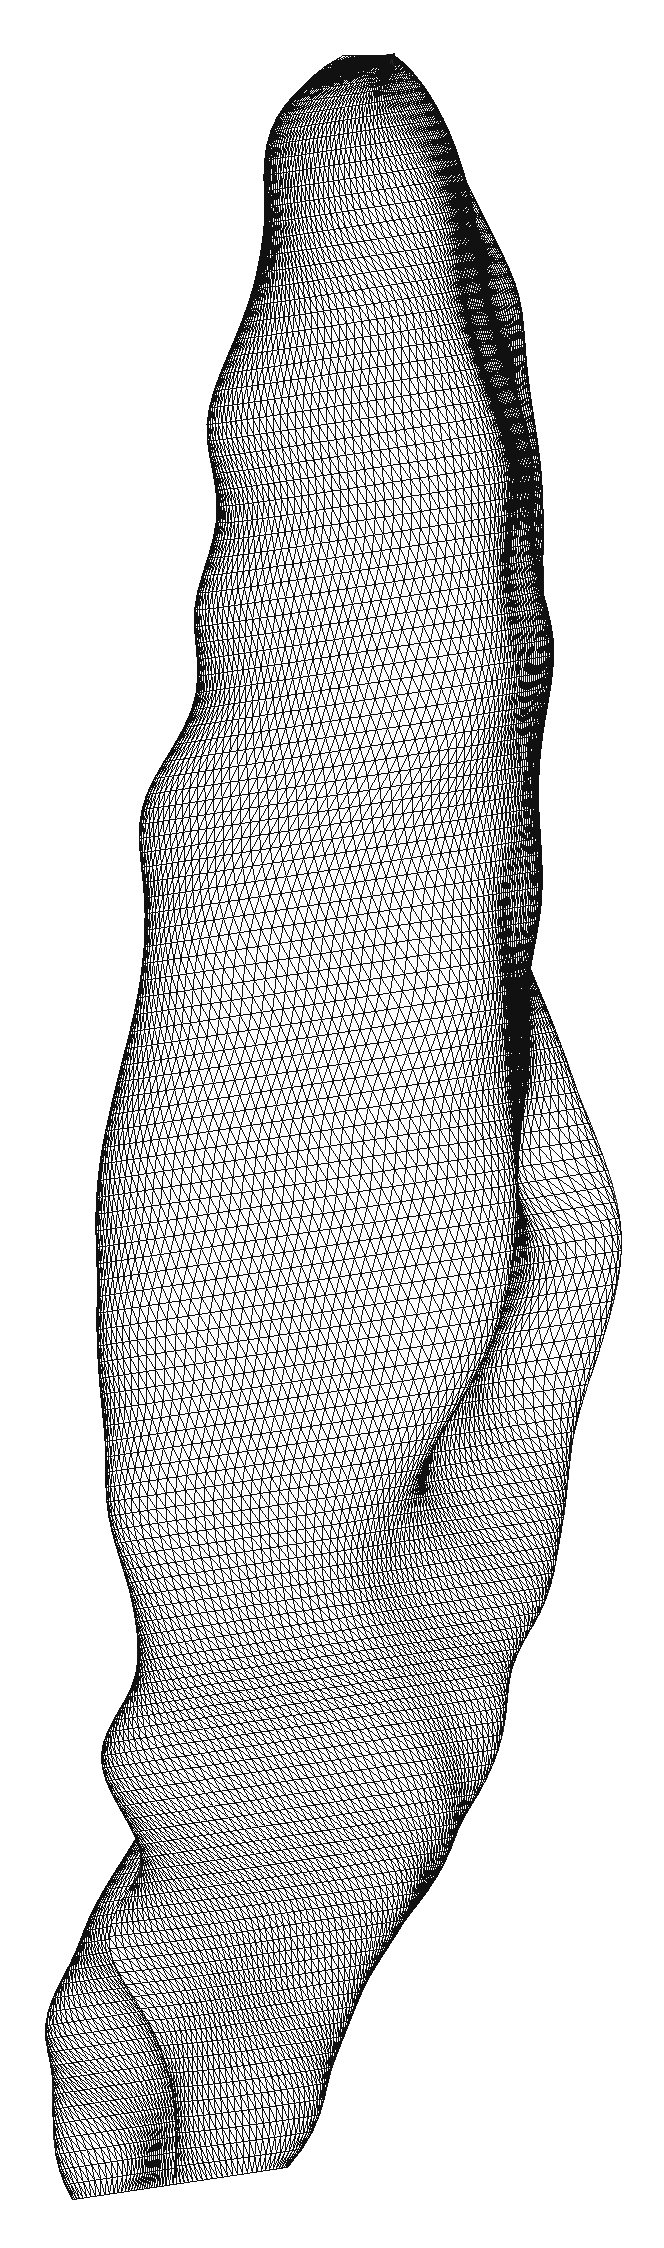
\includegraphics[height=7cm]{images/fiber_creation/extraction_biceps.png}%
    \caption{Surface of the biceps brachii muscle. At the right side of the muscle, the groove of the humerus bone can be seen.}%
    \label{fig:extraction_result_biceps}%
  \end{subfigure}
  \begin{subfigure}[t]{0.48\textwidth}%
    \centering%
    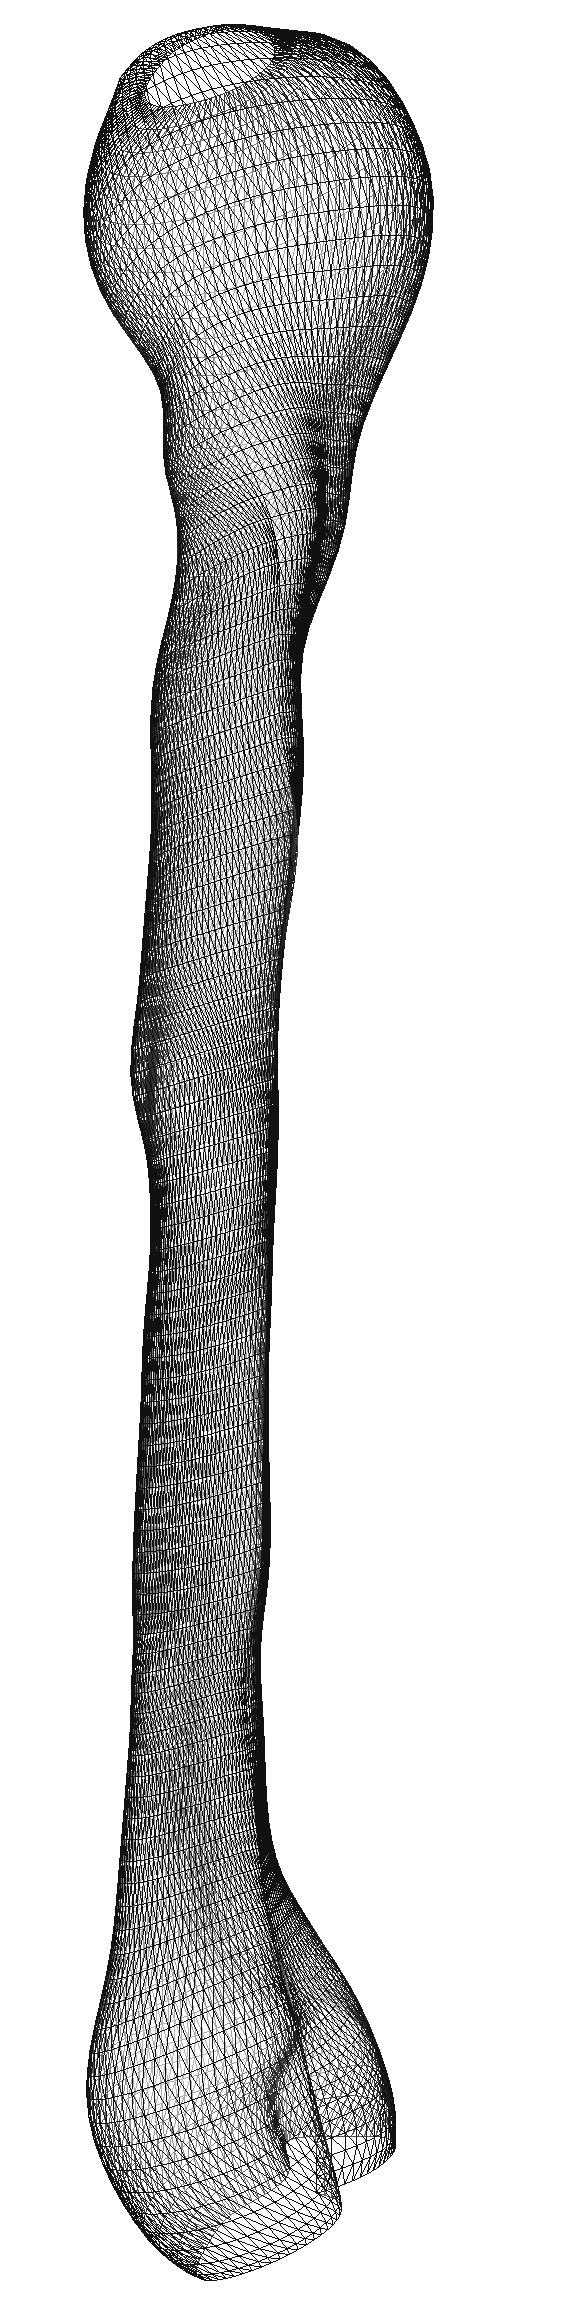
\includegraphics[height=7cm]{images/fiber_creation/extraction_humerus00.png}%
    \caption{Surface of the humerus.}%
    \label{fig:extraction_result_humerus}%
  \end{subfigure}    
  \caption{Surfaces of biceps and humerus bone obtained by the automatic surface extraction algorithm.}%
  \label{fig:extraction_result}%
\end{figure}%

The runtime for the algorithm applied on a dataset with \num{495} images and circa \num{144e6} pixels in total was \SI{121}{\minute}. The used hardware was a AMD Ryzen 5 1600 processor with 6 cores, 3.2 GHz and \SI{16}{\giga\byte} RAM, of which a maximum of \SI{2}{\giga\byte} was used. Because processing of the images can be done in parallel, the runtime was reduced to approximately half (\SI{62}{\minute}) using 2 threads and to a quarter (\SI{30}{\minute}) using 6 threads.

The advantage of the presented algorithm is that the outcome solely depends on the imaging data and, thus, no modeling error by manual approximation of the geometry occurs. For example, the obtained surfaces of biceps and humerus geometrically fit perfectly into each other. Intermediate steps are stored as black and white images. By editing these between the steps of the algorithm, manual tweaking is possible and can be used to increase the quality of the results.

A disadvantage is that the algorithm relies on color information in the imaging data to differentiate between muscle and other tissue. Because some of the involved tissue types have similar colors, this approach can be error-prone. Furthermore, the color ranges need to be determined experimentally. Therefore, the algorithm is not very robust with respect to image noise and needs adjustments when it should be used to extract other muscles. Expert knowledge about the location and shape of human muscles cannot be used easily to improve the results of the algorithm.

An alternative approach is to manually segment the imaging data and construct surfaces with the help of a tool. This approach is described in the following section.

\subsection{Manually Guided Surface Extraction}\label{sec:surf_extr}

Manually guided segmentation can be done using the \emph{MAP client} of the Musculoskeletal Altas Project (MAP) \cite{mapclient}. This application allows to create and execute a workflow to achieve data processing and simulation tasks. In a graphical window, the user can place and connect various workflow steps. When executing the workflow, each step shows a dialog where the required configuration can be entered or the operations can be performed on a visual representation of the data at this workflow stage. 

Possible workflow steps include source and sink operations such as reading image data and writing meshes. Imaging data such as the 2D images from the Visual Human Male can be visualized in a 3D representation. The user can place points in the 3D space to mark boundaries of the visualized muscle and tissue structures.
Further workflow steps allow to create meshes of predefined geometrical shapes, such as cubes and cylinders and merge them into a common mesh. These meshes can be fitted to point clouds of user defined points. This is done by a least squares approach minimizing the distances between user created points and the mesh surface. Details can be found in \cite{Fernandez2018}.

The MAP client has a plugin architecture and allows to create new workflow steps. It imports features from OpenCMISS, especially data processing formats and tools from OpenCMISS Zinc. Meshes can be created with 3D cubic Hermite elements that allow for a high geometric modeling flexibility with a low number of nodes. Such meshes are stored in the OpenCMISS file format of \code{exnode} and \code{exelem} files.

As a result, meshes of individual muscles or the whole human organism can be created. \Cref{fig:vhp_geometry} shows meshes that were create from the cryosectioning data of the Visible Human Male. In \cref{fig:vhp_total}, almost the whole body has been extracted. In \cref{fig:vhp_detail}, the mesh consisting of cubic Hermite elements is visualized. A relatively coarse mesh width suffices to model a smooth surface of the body. When exported in the exfiles format from the MAP client, the data can be visualized, e.g., using \emph{cmgui}, the visualization tool of OpenCMISS Zinc.

\begin{figure}%
  \centering%  
  \begin{subfigure}[t]{0.48\textwidth}%
    \centering%
    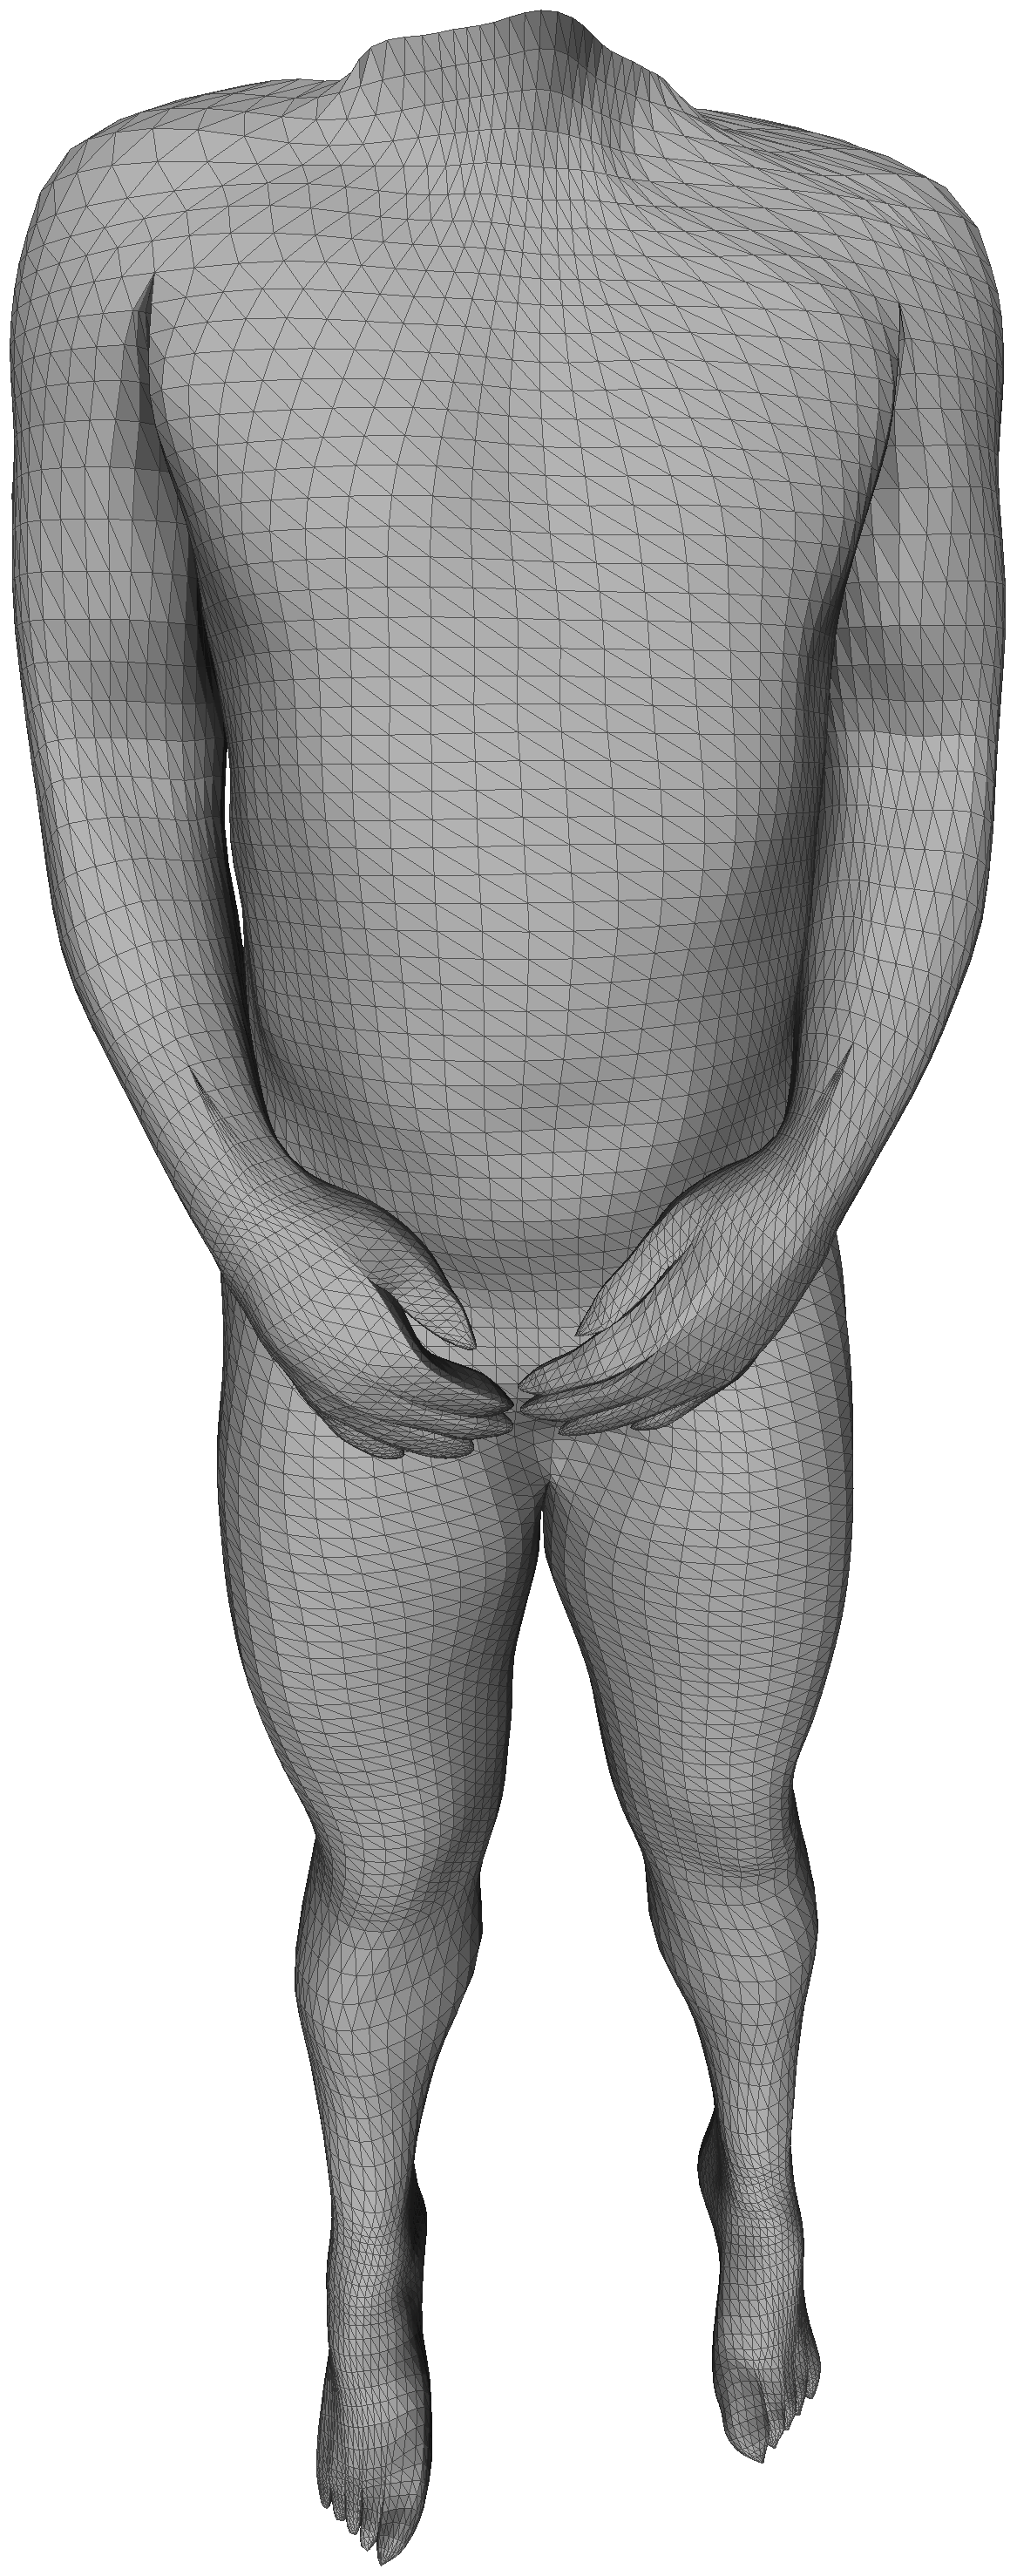
\includegraphics[height=10cm]{images/fiber_creation/skin00.png}%
    \caption{Mesh of the trunk and limbs, the surface has been triangulated for visualization.}%
    \label{fig:vhp_total}%
  \end{subfigure}
  \quad
  \begin{subfigure}[t]{0.48\textwidth}%
    \centering%
    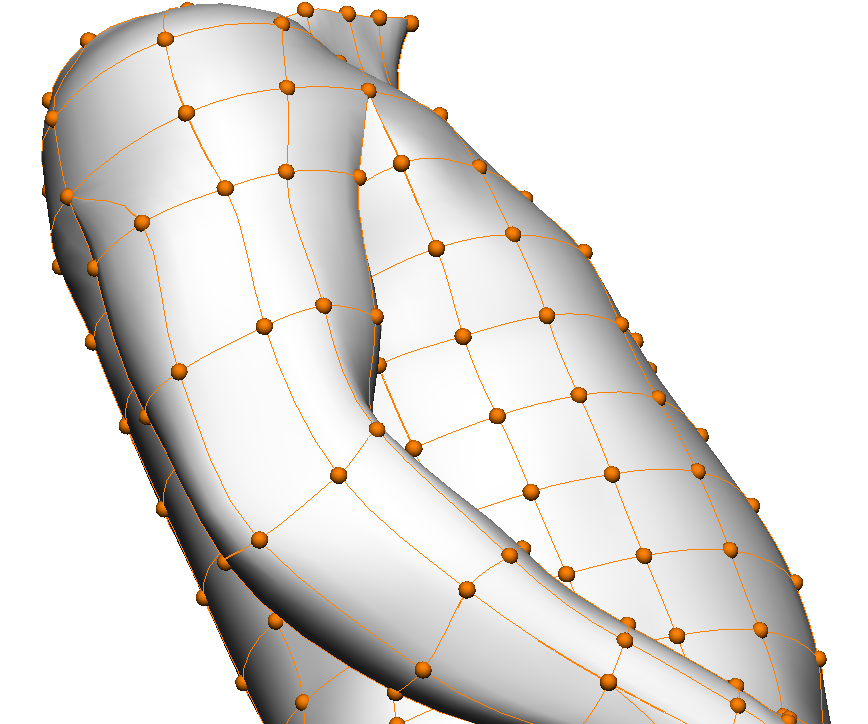
\includegraphics[height=7cm]{images/fiber_creation/elements4_red.png}%
    \caption{Detail view of part of the right upper arm and the trunk with orange nodes and edges of a cubic Hermite element mesh.}%
    \label{fig:vhp_detail}%
  \end{subfigure} 
  \caption{Mesh of the Visible Human Male from the Visible Human Project.}%
  \label{fig:vhp_geometry}% 
\end{figure}%

The mesh width of the meshes obtained using the MAP client was chosen such that the surface fitting yielded good results. The meshes are not necessarily ready for use in a simulation, especially if a  high mesh resolution is desired. 
Apart from the mesh width also the type of elements can be different than what is needed for a Finite Element simulation. Our goal is to obtain meshes with linear or quadratic Lagrange elements with configurable mesh widths for the specified upper arm muscles, such as the biceps brachii.

Therefore, the next step of the workflow, as visualized by the right branch of \cref{fig:scheme_preprocessing}, is to transform the volume mesh into a surface mesh which then can be used as start for further meshing. The further meshing steps are visualized in \cref{fig:biceps_processing}. The start is the Hermite mesh shown in the left-most image.

\begin{figure}%
  \centering%
  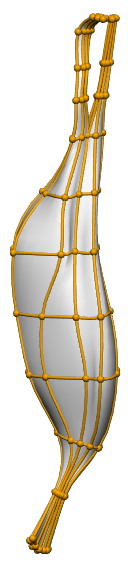
\includegraphics[height=10cm]{images/fiber_creation/exfile_red.png}\quad%
  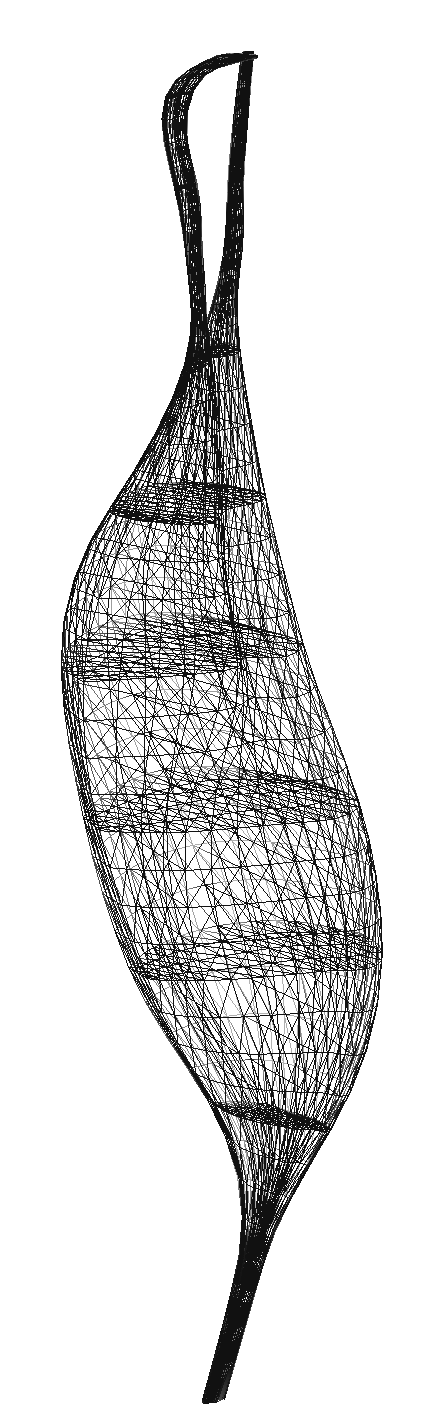
\includegraphics[height=10cm]{images/fiber_creation/biceps23.png}%
  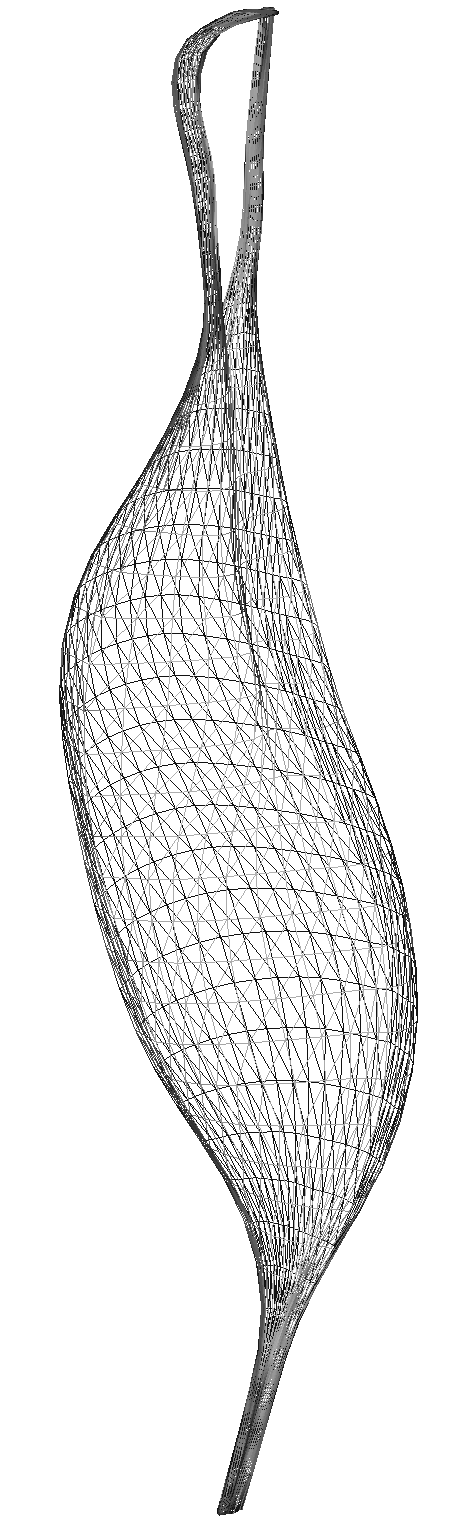
\includegraphics[height=10cm]{images/fiber_creation/biceps22.png}%
  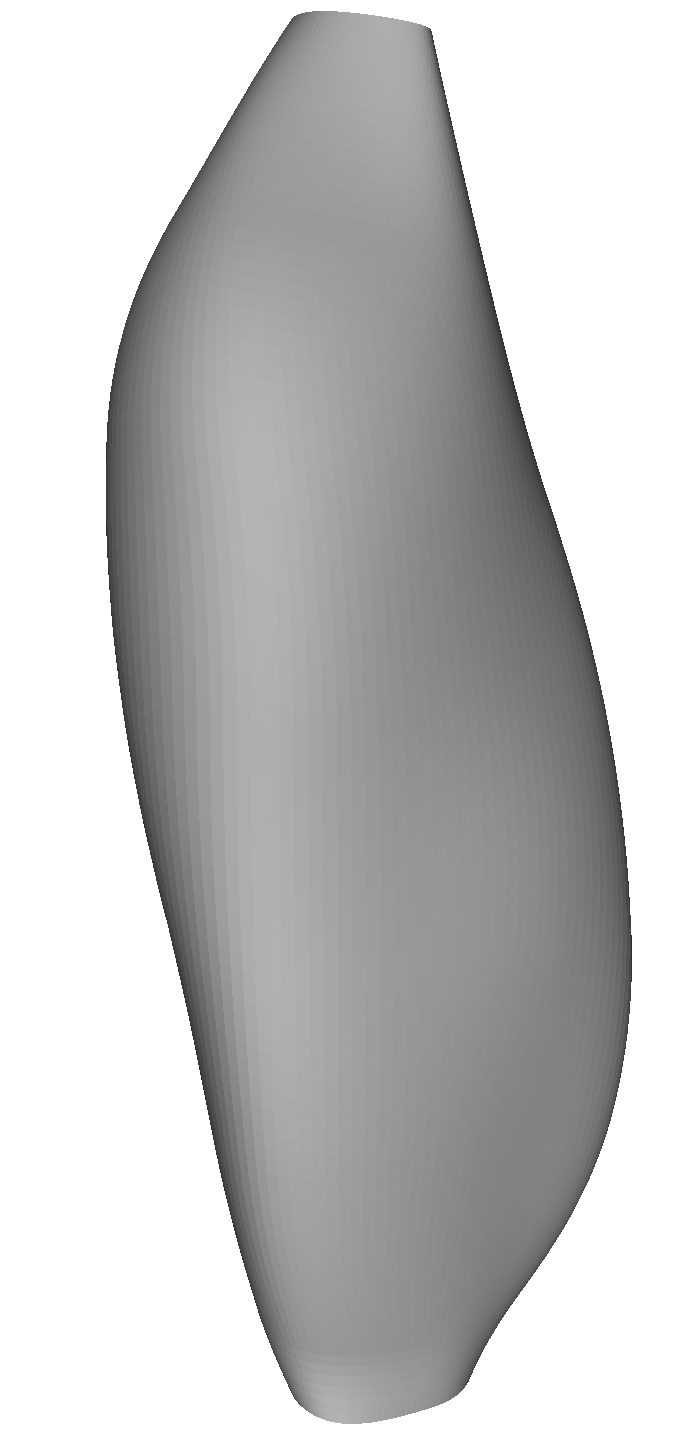
\includegraphics[height=10cm,trim=-2cm 0 0 -2cm, clip]{images/fiber_creation/splines00.png}%
  \caption{Processing the geometry of the biceps brachii muscle. From left to right: mesh with cubic Hermite elements, STL mesh with inside triangles, STL surface mesh where triangles lying inside have been removed, Spline surface of the muscle belly.}%
  \label{fig:biceps_processing}%
\end{figure}%

The Hermite elements can be triangulated and stored as an STL file using the tool \mbox{\code{cmgui}.} This process triangulates the non-planar faces of all Hermite elements. This leads to a dataset with triangles both on the surface and in the inside of the volume, as can be seen in the second image of \cref{fig:biceps_processing}. At this stage, the use of the MAP and OpenCMISS related tools is finished and further processing steps are performed using tools from \opendihu{} that we developed on our own.

A Python script removes the triangles inside the volume. The detection whether a triangle is inside the volume is done by casting four rays from the center of gravity of the respective triangle and determining if the rays intersect any other triangles. The rays have directions $(x,y,z) = (\pm1,\pm1,\frac13)$, where the $z$ axis is oriented along the muscle's longitudinal axis and the $x$ and $y$ axes are oriented in radial direction. The ray-triangle intersection is done using the fast Möller-Trumbore algorithm \cite{ray-triangle}. For every ray, all triangles are checked.
Only if all four rays intersect at least one more triangle, the starting triangle is considered to be inside the volume and subsequently removed from the dataset. 

This algorithm has a quadratic time complexity $\O(n^2)$ in the number of triangles $n$. It could be improved by organizing the triangles in a spatially adaptive data structure, such as an octree. However, since this preprocessing step has to be performed only once for a given geometry, the runtime is not critical and there is no need for such optimization.

The result of this operation is a triangulated surface, shown in the third image of \cref{fig:scheme_preprocessing}. The next step is to create a Spline surface of the muscle belly, as shown in the right-most image of \cref{fig:scheme_preprocessing}. This is described in the next two sections.

\subsection{Introduction of Spline Surfaces}\label{sec:nurbs}
After the surface representation of the muscle has been obtained from either the left or the right branch of the preprocessing workflow in \cref{fig:scheme_preprocessing}, the surface is given by a point cloud or a number of triangles. To remedy eventual outliers or unphysiological sharp edges from the segmentation, a Spline surface is fitted to the data. This leads to a smooth surface representation and later to a better conditioned Finite Element mesh in the simulation. However, this step is optional. It is also possible to directly use the surface triangulation from \cref{sec:surf_extr} for the meshing algorithm described in \cref{sec:ser_alg_meshes}.

The surfaces use Nonuniform Rational B-splines (NURBS). A NURBS surface is a generalization of a B-spline surface. From a modeling point of view, B-spline surfaces have three advantageous properties.
First, the B-spline surface can be constructed with given smoothness properties.  
Second, the definition of a particular B-spline surface builds on intuitive geometric information, which simplifies their creation: A control polygon mesh in 3D space is defined. Its convex hull is guaranteed to contain the surface.
Third, the geometric parameters of a B-spline surface have only local impact on the shape of the surface. This allows a B-spline surface of a fixed, low polynomial degree to approximate point clouds with any number of points without loosing approximation quality.

A limitation of B-spline surfaces is that circular and spherical shapes cannot be represented. This limitation is overcome by NURBS surfaces. NURBS surfaces are defined as the perspective projection into 3D space of a B-spline surface in 4D space.

The mathematical description is given in this section, following the notation of \cite{piegl2012nurbs}. The building blocks are the B-spline basis functions of polynomial degree $p$. Given a knot vector 
%
\begin{align*}
  \Xi = (\xi_1, \xi_2, \dots, \xi_k) \in \R^k \quad \text{with } a=\xi_1 \leq \xi_2 \leq \cdots \leq \xi_k = b,
\end{align*}
%
the $i$th B-spline basis function $N_{i,n}$ of degree $n$ is defined recursively starting with the piecewise constant function
%
\begin{align*}
  N_{i,0}(\xi) = \begin{cases} 
    1 \, &\text{for }\xi_i \leq \xi < \xi_{i+1},\\[2mm]
    0 &\text{else},
  \end{cases}
\end{align*}
and using the following relation to define the functions of higher degree $(n > 0)$:
\begin{align*}
  N_{i,n}(\xi) = \dfrac{\xi - \xi_i}{\xi_{i+n} - \xi_i} N_{i,n-1}(\xi) + \dfrac{\xi_{i+n+1} - \xi}{\xi_{i+n+1} - \xi_{i+1}} N_{i+1,n-1}(\xi), \quad \text{for all }i > 0.
\end{align*}
Because neighboring entries in the knot vector can be equal, the fraction $0/0$ can occur. In this case, $0/0 := 0$ is defined. Note that by construction of $N_{i,n}$ a zero denominator implies that also the dividend is zero.

A B-spline curve $\bfC: \R \to \R^d$ of polynomial degree $p$ is defined as
%
\begin{align*}
  \bfC(u) = \s{i=1}{l}N_{i,p}(u)\,\bfP_i, \quad u \in [a,b].
\end{align*}
%
The coefficients $\bfP_i \in \R^d, i=1, \dots, l$, of the basis functions $N_{i,p}$ are called \emph{control points} and define the control polygon. The number $l$ of basis functions and control points is determined from the number of knots $k$ in an open knot vector and the polynomial degree $p$ as $l = k-p-1$.

The number of equal entries in series in the knot vector is the \emph{multiplicity} of the respective knot value. Usually \emph{open} knot vectors $\Xi$ are used where the first and the last knot occur with a multiplicity of $p+1$.
This makes the first and the last points of the B-spline curve coincide with the control polygon points: $\bfC(a) = \bfP_1$ and $\bfC(b) = \bfP_l$.

The multiplicities of the knots in the knot vector encode information about the smoothness of the B-spline curve. If the knot value $\hat{\xi}$ has a multiplicity of $m$, the B-spline curve will be $(p-m)$ times continuously differentiable at $\bfC(\hat{\xi})$.
% This can be seen from the fact that there exist $m$ basis functions with a support that begins at $\hat{\xi}$.

An exemplary B-spline curve is shown in \cref{fig:bspline_curve}. It uses a \emph{non-uniform} knot vector for polynomial degree $p=3$, where the differences $\xi_{i+m} - \xi_i$ between neighboring knot values vary. The effect of different multiplicities can be seen. The multiplicity $m=p=3$ places the point of the curve at the knot on the respective control point, as for $\xi=49$ in the example. The multiplicity $m=p-1=2$ places the point of the curve at the knot on the control polygon, as in the example at $\xi=10$. A lower multiplicity $m < p-1$ does not yield a higher smoothness and in turn does not force the curve to coincide with the control polygon at the respective knot. It can also be seen that the B-spline curve stays inside the convex hull of the control polygon which is a property of B-spline curves \cite{piegl2012nurbs}.

\begin{figure}%
  \centering%
  \def\svgwidth{8cm}%
  \input{images/fiber_creation/bspline_curve.pdf_tex}%
  \caption{Exemplary B-spline curve (red) of degree $p=3$ for the knot vector $\Xi = (0,0,0,0,7,10,10,49,49,49,50,50,50,50)$, control points (blue) and control polygon (black).
  Positions of the curve $\bfC(\xi_i)$ at the knots $\xi_i$ are indicated by the red squares and the knot value $\xi$ and its multiplicity $m$ is given. The effect of moving one control point is shown in green.}%
  \label{fig:bspline_curve}%
\end{figure}%
%
The effect of moving one of the 10 control points is visualized with green color in \cref{fig:bspline_curve}.
The B-spline basis function $N_{i,p}$ has a local support of $S=(\xi_i,\xi_{i+p+1})$. Consequently, only the corresponding part of the curve, $\bfC(\xi)$ for $\xi \in S$, changes.

A B-spline surface $\bfS : \R^2 \to \R^d$ is given by the tensor product of two B-spline curves:
\begin{equation}\label{eq:bspline_surface}
  \begin{array}{lll}
    \bfS(u,v) = \s{i=1}{l^{(1)}}\s{j=1}{l^{(2)}} N^{(1)}_{i,p^{(1)}}(u)\,N^{(2)}_{j,p^{(2)}}(v)\, \bfP_{i,j}.
  \end{array}
\end{equation}

Here, we have two polynomial degrees $p^{(1)}$ and $p^{(2)}$, the ansatz functions $N^{(1)}_{i,p^{(1)}}$ and $N^{(2)}_{j,p^{(2)}}$ with $l^{(1)}$ and $l^{(2)}$ ansatz functions per coordinate direction are constructed from the corresponding knot vectors per coordinate direction.

NURBS, B-spline curves and surfaces are formulated using \emph{homogeneous coordinates}. Every point in Cartesian coordinates $(x,y,z) \in \R^3$ has a set of homogeneous coordinates $(\tilde{x},\tilde{y},\tilde{z},w)=(x\,w,y\,w,z\,w,w)$. Thus, the Cartesian coordinates can be obtain from the homogeneous coordinates by the \emph{perspective division}, i.e., dividing all but the last coordinate by the weight $w$.

A NURBS surface is given by the same definition as the B-spline surface in \cref{eq:bspline_surface} except that the control points $\bfP_{i,j} \in \R^3$ are enriched with scalar weights $w_{i,j}$ and, thus, replaced by $(\bfP_{i,j}, w_{i,j}) \in \R^4$. The resulting surface $\bfS$ is given in homogeneous coordinates. Executing the perspective division yields the form:
%
\begin{align*}
  &\bfT(u,v) = \s{i=1}{l^{(1)}}\s{j=1}{l^{(2)}} R_{i,j}(u,v) \,\bfP_{i,j},\\[4mm]
  &\text{with } R_{i,j}(u,v) = \dfrac{N_{i,p^{(1)}}(u)\,N_{j,p^{(2)}}(v)\,w_{i,j}}{\s{r=1}{l^{(1)}}\s{s=1}{l^{(2)}} N_{r,p^{(1)}}(u)\,N_{s,p^{(2)}}(v)\,w_{r,s}}.
\end{align*}
The new rational basis functions $R_{i,j}$ and the possibly non-uniform knot vectors give rise to the name Non-Uniform Rational B-spline surface (NURBS).

\subsection{Fitting a Spline Surface to the Muscle Geometry}
In order to find a NURBS surface for the given triangulated surface of a muscle, at first, the part of the geometry corresponding to the tendons is removed such that the resulting triangles model only the surface of the muscle belly. In our example of the biceps muscle, the resulting belly has a length of \SI{12.8}{\mm}.

Then, twelve cross sections are extracted from the surface triangles. As a result, we get twelve horizontal circumferential rings. On each ring, 9 equidistant points are determined. The first point is appended after the last point in every ring, such that in total we obtain a grid of $10 \times 12$ points. 

Then, the least squares surface approximation algorithm by \cite{piegl2012nurbs} is used to fit a NURBS surface to the points. The implementation of the algorithm is given by the NURBS-Python (geomdl) library. Polynomial degrees of $p^{(1)} = 3$ and $p^{(2)}=2$ are used where the first dimension corresponds to the cross-sectional direction of the muscle. The knot multiplicity is chosen as $m=1$ for both coordinate directions. We obtain a two times respective one times continuously differentiable surface in $u$ and $v$ direction. 
The resulting NURBS surface and the control polygon are visualized in \cref{fig:biceps_splines_control_points}. Note that the control polygon is different from the grid of points against which the surface is fitted.
%
\begin{figure}%
  \centering%
  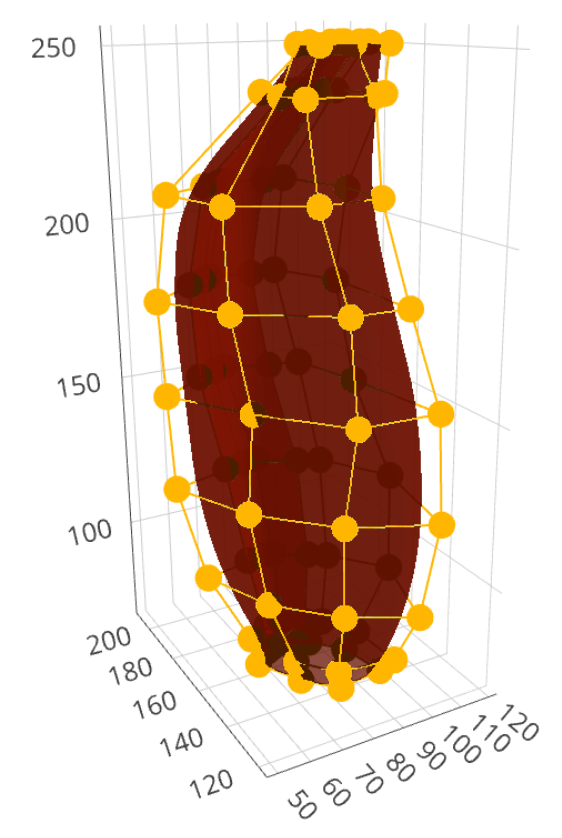
\includegraphics[width=0.35\textwidth]{images/fiber_creation/splines01red.png}%
  \caption{Muscle surface description with Splines: Fitted NURBS surface of the biceps muscle (red) and the control polygon (orange).}%
  \label{fig:biceps_splines_control_points}%
\end{figure}%

\Cref{fig:biceps_splines_wrong} shows the result of this approach in more detail. We observe that the surface is non-differentiable and has a kink at the seam line where the first and last points of each ring meet. The reason for this is that the surface fitting algorithm does not pose any conditions on the tangents at the edges of the fitted NURBS surface.  Thus, the tangents mismatch.

Since no implementation of a fitting algorithm specifically for a tubular NURBS surface with periodicity in tangential direction is available, we develop a different remedy. We modify the point grid that is used for the surface fitting. The series of 9 equidistant points on each ring is replicated twice and the first point is again added as the last point. This leads to a grid of $(3\cdot 9+1) = 28 \times 12$ points which wrap around the muscle volume in cirumferential direction three times. The NURBS surface fitting algorithm is applied on this grid. The resulting NURBS surface also wraps around the muscle three times with the two ends being again not properly fitting to each other. From these three wraps, the middle one is extracted. In the biceps example, this corresponds to restricting the NURBS surface $\bfT(u,v)$ from $(u,v) \in [0,1]^2$ to $(u,v) \in [0.4,0.733]\times [0,1]$.

The result is depicted in \cref{fig:biceps_splines_seam}. The tangents now match very well between the two sides of the NURBS surface. Additionally, the comparison with the inital approach in \cref{fig:biceps_splines_wrong} shows that an artifical bulge at the top of the muscle in the perspective of the visualization is removed. The overall shape of the muscle now looks smoother and more natural. Also, a comparison with the result of the automatic algorithm given in \cref{fig:extraction_result_biceps} shows that the results of our new approach are smoother.

The generated tubular surface has two holes at the top and bottom which prevent it from being an enclosing surface to the muscle belly volume. The borders of these holes each lie in a plane and, thus, the missing surfaces are treated as being planar during the subsequent creation of the 3D meshes.

For the next step, a triangulation of the tubular surface is created and stored as STL mesh file. We use the respective functionality of the NURBS-Python library that creates a structured triangle mesh using the 2D parametrization of the NURBS surface.

%
\begin{figure}%
  \centering%
  \begin{subfigure}[t]{0.48\textwidth}%
    \centering%
    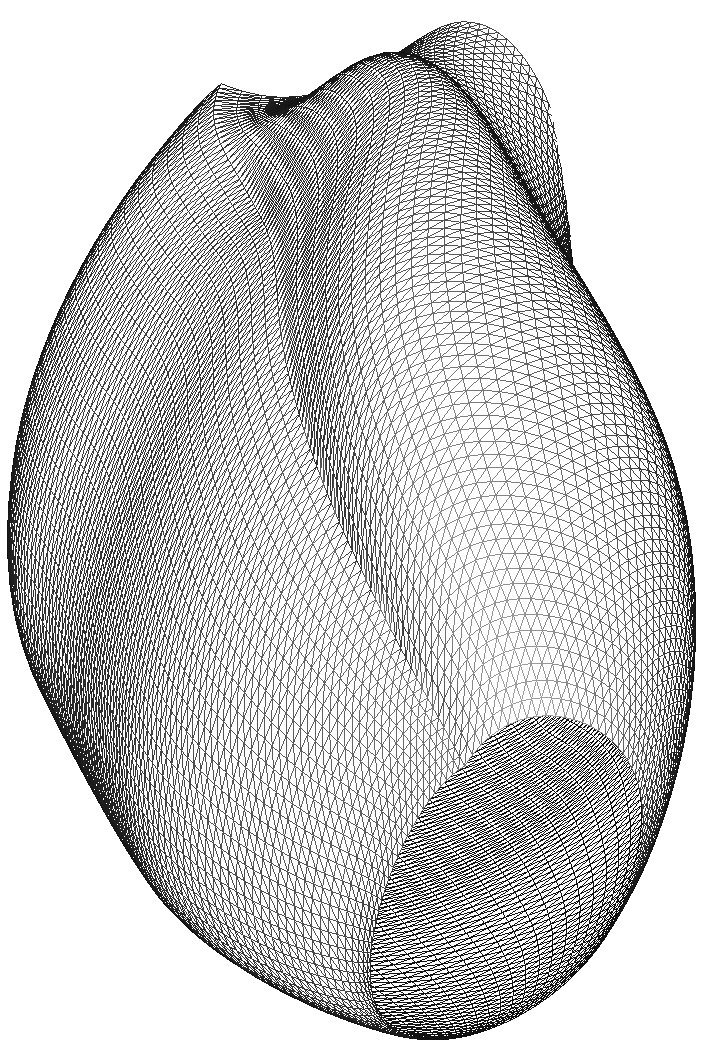
\includegraphics[height=8cm]{images/fiber_creation/splines_wrong00.png}%
    \caption{First approach with $10 \times 12$ control points. The kink at the seam line along the muscle is clearly visible.}%
    \label{fig:biceps_splines_wrong}%
  \end{subfigure}
  \quad
  \begin{subfigure}[t]{0.48\textwidth}%
    \centering%
    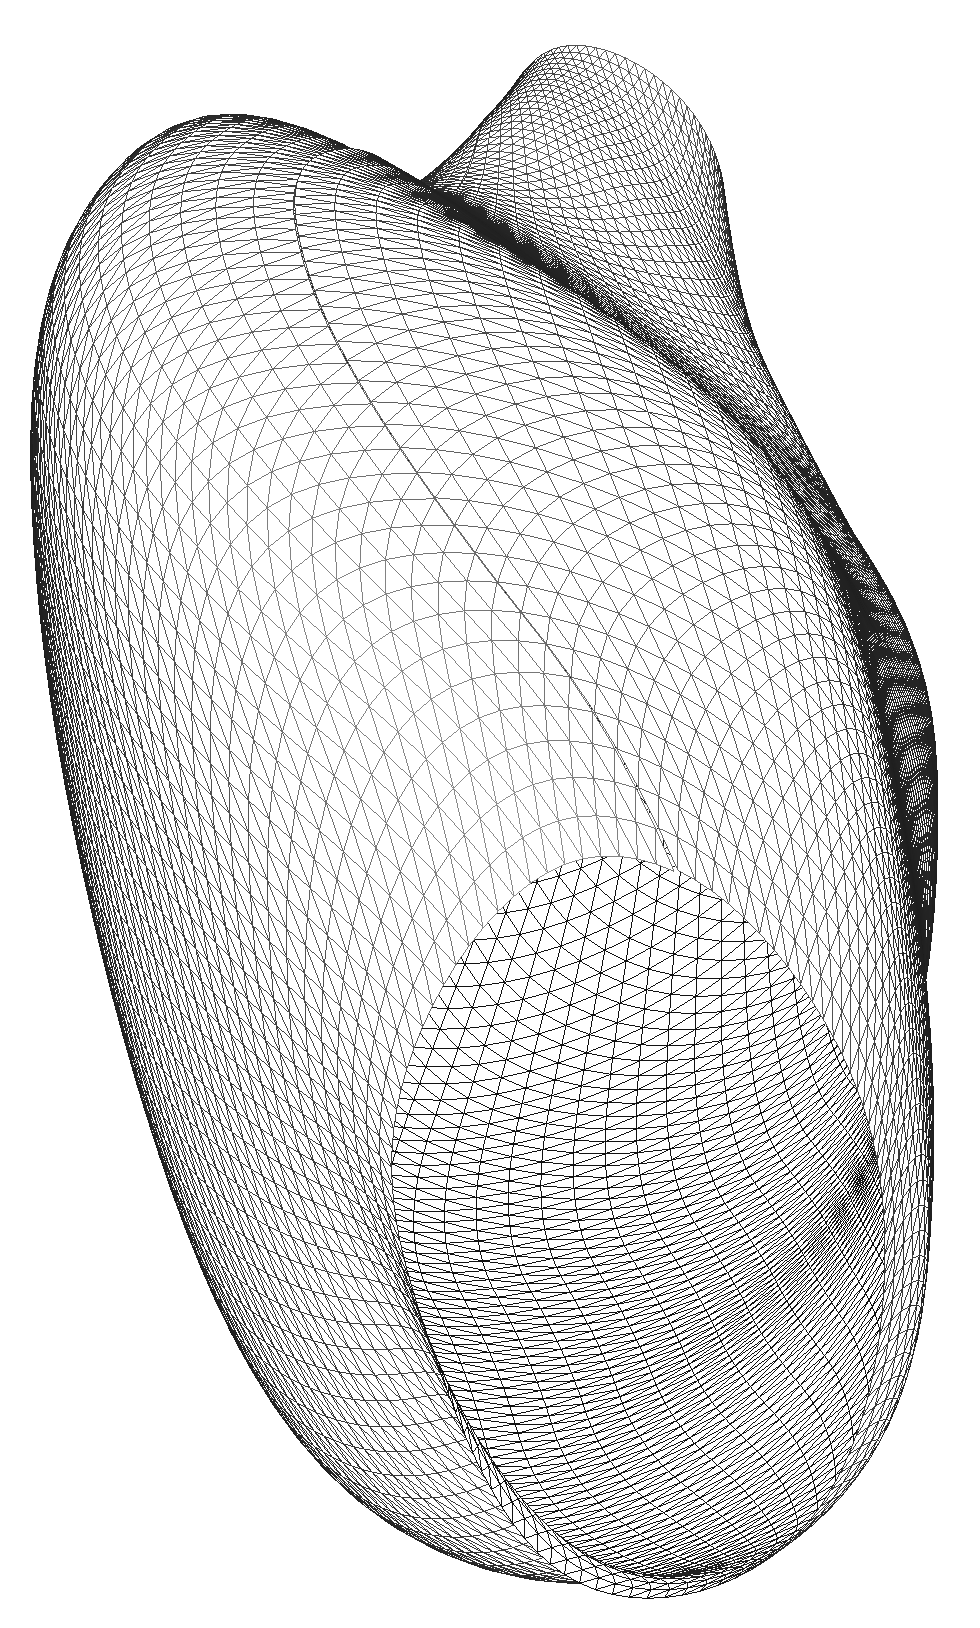
\includegraphics[height=8cm]{images/fiber_creation/splines_seam00.png}%
    \caption{Second, improved approach with $28 \times 12$ points. It can be seen that the tangents at the seam line match very well.}%
    \label{fig:biceps_splines_seam}%
  \end{subfigure}
  \caption{Muscle surface description with Splines: Fitted NURBS surface of the biceps muscle, triangulated for visualization purposes.}%
  \label{fig:biceps_splines}%
\end{figure}%
%
\section{Serial Algorithm to Create Muscle and Fiber Meshes}\label{sec:ser_alg_meshes}
Next, a 3D mesh for the muscle volume and 1D meshes for muscle fibers need to be generated from the surface representation described in the previous sections. In this section, first an algorithm for the 3D mesh is described. Then, a second algorithm that reuses results from the first algorithm is presented which generates one dimensional meshes for muscle fibers. Both algorithms are executed in serial. A derived algorithm that can run in parallel and, thus, can handle larger datasets on a distributed memory hardware is presented in \cref{sec:parallel_algorithm}.

The steps of a serial algorithm for the generation of a 3D mesh are given in \cref{alg:serial_algorithm_1}. Input is the set of triangles at the tubular surface of the muscle. The tubular surface is oriented along the $z$ axis. In the following descriptions, the muscle in considered to be oriented upright such that the $z$ axis points in vertical direction towards the top. The borders at the bottom and at the top have a constant $z$ coordinate.
%
\begin{algorithm}
  \begin{algorithmic}[1]%
    \Procedure{Create\_3D\_mesh}{}
    \Require Triangulated tubular surface
    \Ensure Structured 3D volume mesh
    \Statex
    \State Slice geometry           \label{alg:1.1}
    \State Triangulate 2D slices      \label{alg:1.2}
    \State Compute harmonic maps $u, v$ from the slices to a parameter space     \label{alg:1.3}
    \State Construct regular grid in parameter space and map it to slices            \label{alg:1.4}
    \State Form 3D quadrilateral elements between the 2D slices’ meshes   \label{alg:1.5}
    \EndProcedure
  \end{algorithmic}%
  \caption{Serial algorithm for generation of 3D meshes}%
  \label{alg:serial_algorithm_1}%
\end{algorithm}%

The idea of the algorithm is to first create 2D meshes with good quality on cross-sectional slices of the muscle volume and then combine them to get a 3D mesh. The algorithm starts with creating the horizontal 2D slices in lines \ref{alg:1.1} and \ref{alg:1.2}. The slices get vertically connected at the end of the algorithm in line \ref{alg:1.5} to create the 3D mesh. This step is visualized in \cref{fig:serial_alg_8}. 

Because the goal is to create a hexahedral mesh, the horizontal slices have to consist of quadrilaterals. 
Decomposing a 2D domain into quadrilaterals is easier for a square or circular shaped domain than for an actual cross-section of the muscle. Therefore, we introduce a separate, square or circular shaped parameter domain for creating the quadrilaterals.

\Cref{fig:harmonic_map_solution} outlines the method.
We start at the upper left of the figure with a triangulation on the cross-sectional slices of the muscle. A mapping from the muscle slices to the parameter space at the right of the figure is computed. We use harmonic maps to ensure a smooth mapping that results in good mesh quality. This first steps corresponds to line \ref{alg:1.3} in \cref{alg:serial_algorithm_1}. Different parameter domains such as unit circle and unit square are considered, as shown in \cref{fig:harmonic_map_solution}. It can also be seen at the upper right that the image of the muscle slice triangulation in the parameter domain is better in the unit circle than in the unit square. Therefore, an investigation of different parameter domains and triangulation schemes is necessary.

Next, line \ref{alg:1.4} of \cref{alg:serial_algorithm_1} defines a quadrangulation in the parameter space, shown at the lower right of \cref{fig:harmonic_map_solution}. The quadrilateral elements are mapped back to muscle slices where they are needed for the final 3D mesh. An optional smoothing step at the lower left of the figure further improves the mesh quality.
All steps of the algorithm are described in more detail in the following sections.

\begin{figure}%
  \centering%
  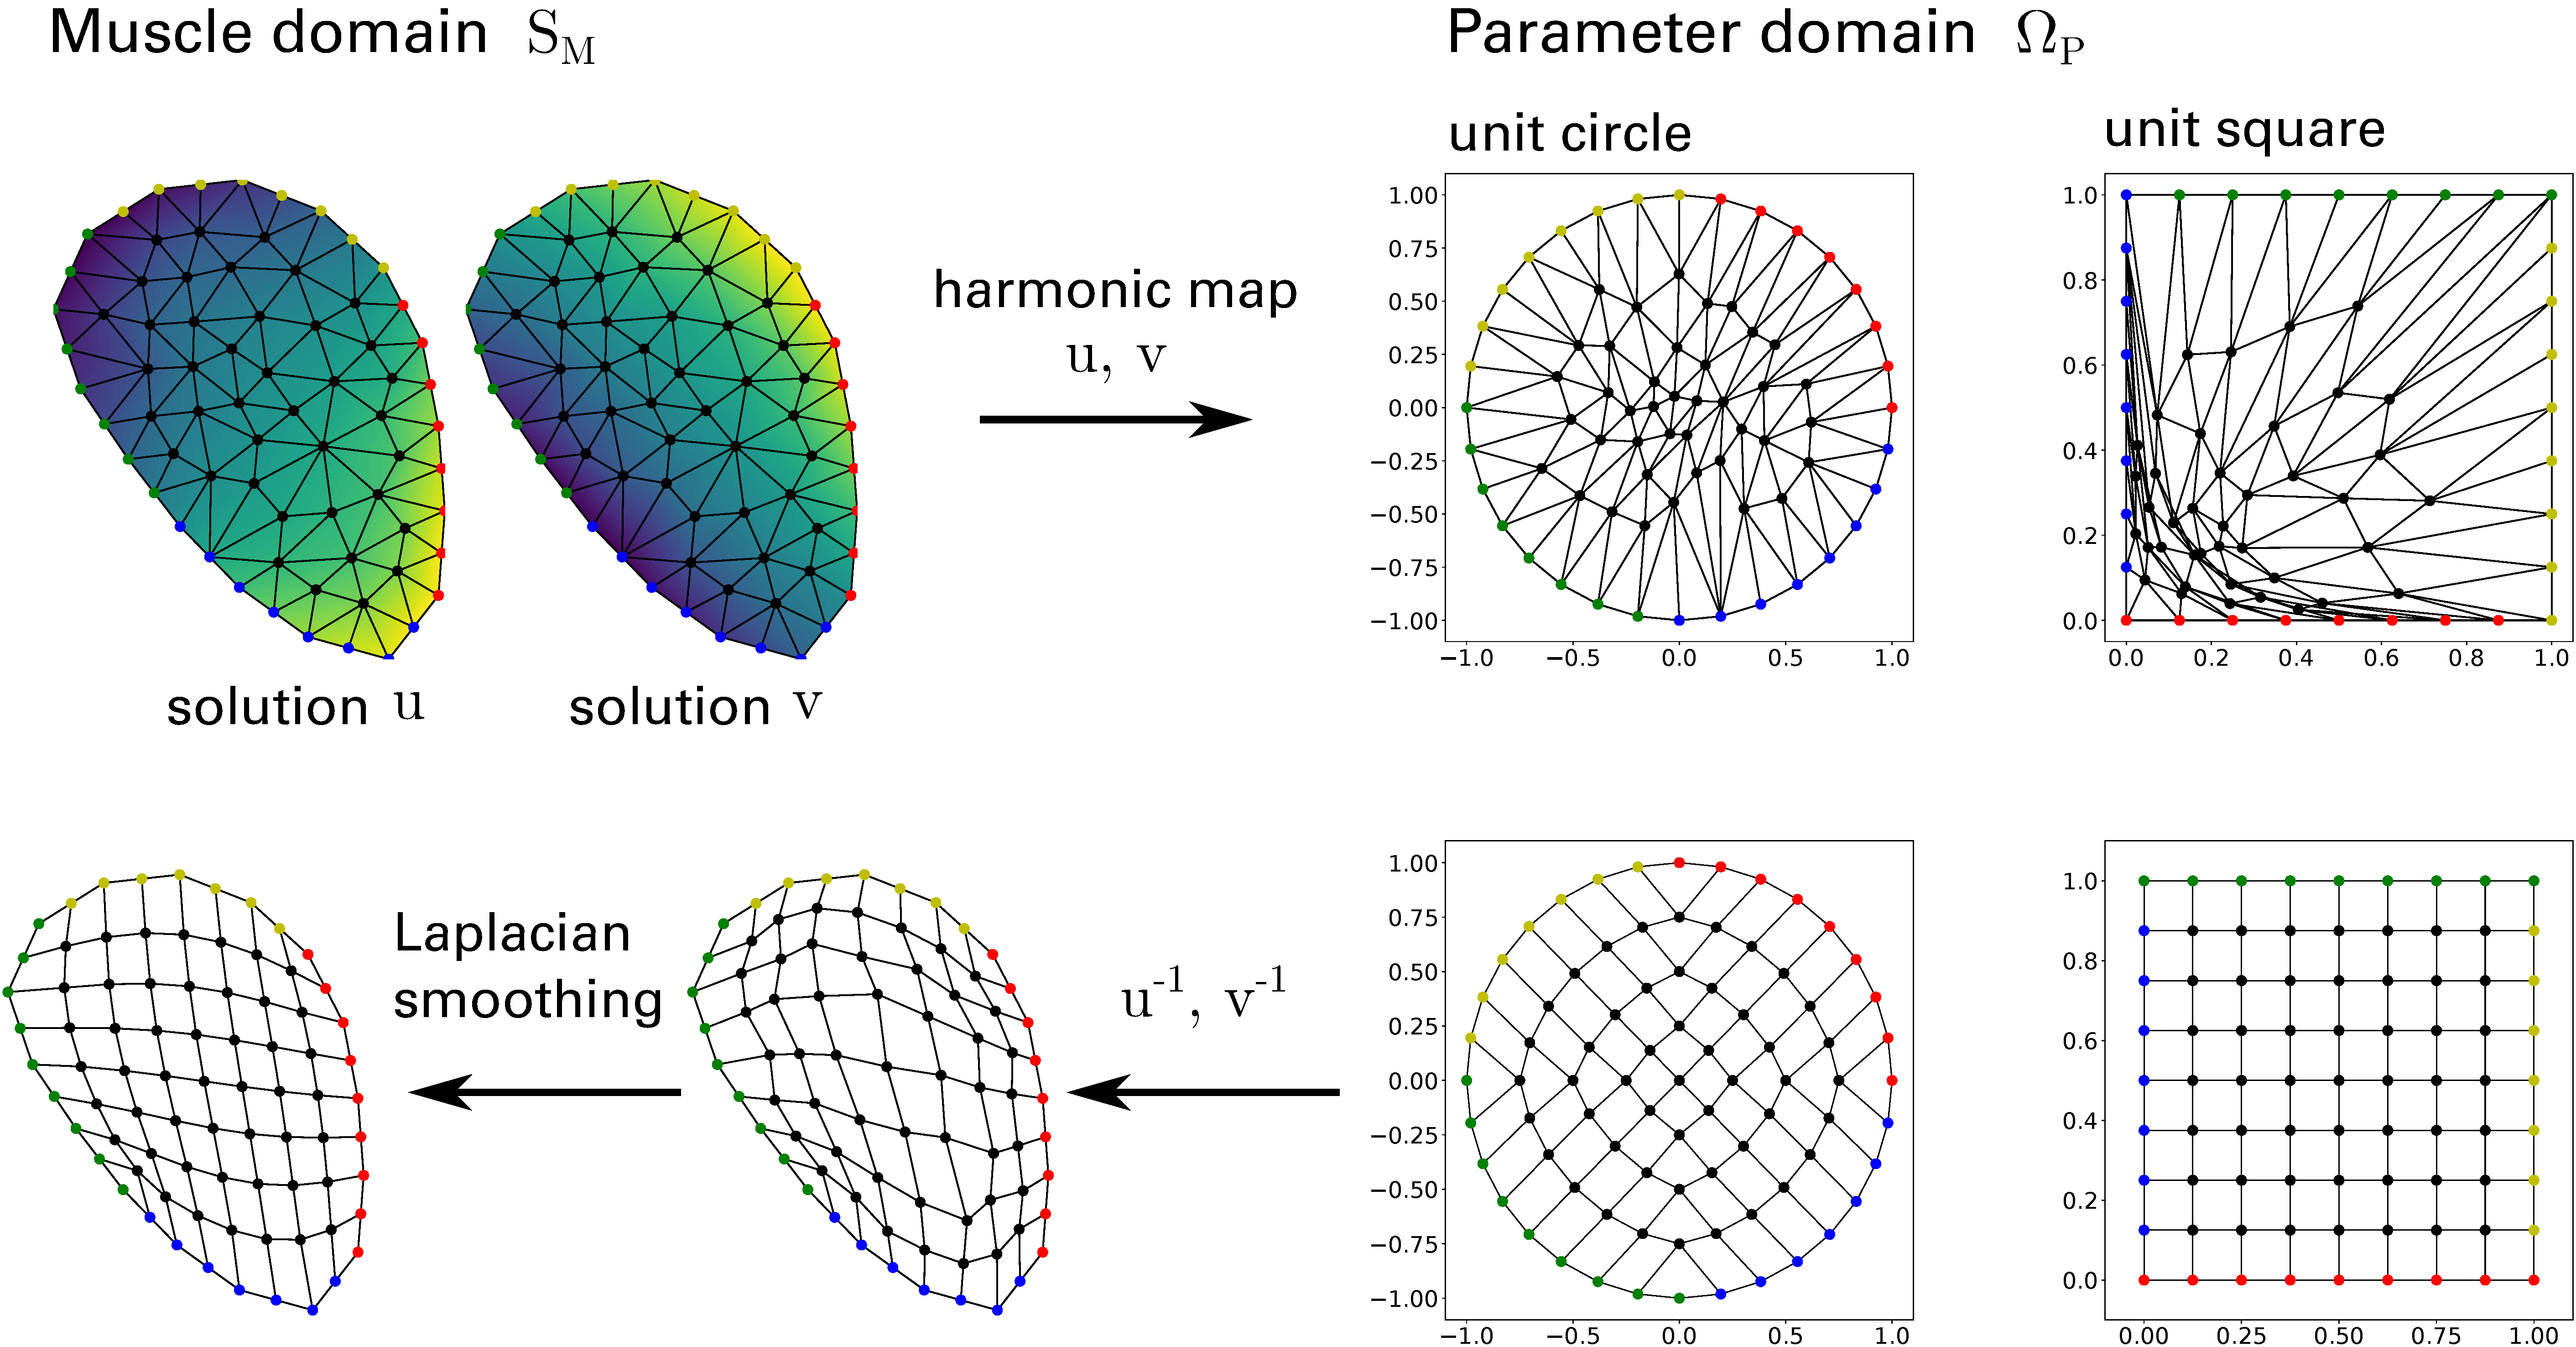
\includegraphics[width=\textwidth]{images/fiber_creation/harmonic_map_scheme_circle_square.pdf}%
  \caption{Generation of the muscle meshes, overview of the mapping method between the muscle domain (left) and the parameter domain (right) using harmonic maps.}%
  \label{fig:harmonic_map_solution}%
\end{figure}%

\subsection{Slicing of the Geometry}\label{sec:slicing_of_the_geometry}
The first step in line \ref{alg:1.1} of \cref{alg:serial_algorithm_1} slices the geometry. This means that horizontal \emph{slices} of the cross-sectional area are extracted from the surface mesh. First, the muscle is divided into equidistant positions $z_i, i=1,\dots,n$ along the $z$-axis where the slices are to be extracted. As can be seen in \cref{fig:serial_alg_0}, $n=13$ $z$ coordinates are selected. Next, for every position $z_i$, all surface triangles $T_j$ that intersect the plane $Z_i = \{\bfp=(x,y,z) \mid z=z_i$\} are considered and the intersection lines $P = T_j \cap Z_i$ are computed. The method of computing plane-triangle intersection is described in the following.

Given is a triangle $T$ with points $\bfp^{1},\bfp^2,\bfp^3 ∈ \R^3$ and a value $\hat{z}$, the result is the set of points $P = T ∩ \{\bfp = (\bfp_x,\bfp_y,\bfp_z) \mid \bfp_z=\hat{z}\}$ which corresponds to a line segment $\overline{\bfp^a\bfp^b}$. 

We describe the points in the triangle by two barycentric coordinates $\xi_1$ and $\xi_2$ as
\begin{equation}\label{eq:barycentric_triangle}
  \begin{array}{lll}
    \bfp(ξ_1,ξ_2) = (1-ξ_1-ξ_2)\,\bfp^{1} + \xi_1\,\bfp^{2} + \xi_2\,\bfp^{3},  \\[4mm]
    \text{with }\xi_1+\xi_2 \leq 1, \quad 0 \leq \xi_1,\xi_2 \leq 1.
  \end{array}
\end{equation}
$\bfp_z(ξ_1,ξ_2) = \hat{z}$ defines the equation for the line through the points $\bfp^a$ and $\bfp^b$ in barycentric coordinates. The solution is given as
\begin{equation*}
  \begin{array}{lll}
    ξ_1 = m\cdot ξ_2 + c,\quad
    m = -\dfrac{\bfp_z^{3} - \bfp_z^{1}}{\bfp_z^{2} - \bfp_z^{1}}, \quad c = \dfrac{\hat{z} - \bfp_z^{1}}{\bfp_z^{2} - \bfp_z^{1}}, \quad \bfp_z^2 \neq \bfp_z^1.
  \end{array}
\end{equation*}
For $\bfp_z^1 = \bfp_z^2 \neq \bfp_z^3$ we swap $\bfp_z^2$ and $\bfp_z^3$.

%
%  # x(xi1,xi2) = (1-xi1-xi2)*x^{1} + xi1*x^{2} + xi2*x^{3},  xi1+xi2 <= 1, 0 <= xi1,xi2 <= 1
%  # x_3(xi1,xi2) = z_value  =>  (1-xi1-xi2)*x^{1} + xi1*x^{2} + xi2*x^{3} = z_value
%  #                         =>  xi1*(x^{2} - x^{1})  +  xi2*(x^{3} - x^{1})  =  z_value - x^{1}
%  #                         =>  xi2 = ((z_value - x^{1}) - xi1*(x^{2} - x^{1})) / (x^{3} - x^{1})
%  #                         =>  xi2 = (z_value - x^{1})/(x^{3} - x^{1}) - xi1 * (x^{2} - x^{1})/(x^{3} - x^{1})
%  #                         =>  xi1 = (z_value - x^{1}) / (x^{2} - x^{1})  - xi2 * (x^{3} - x^{1}) / (x^{2} - %x^{1}) 
Next, the end points of the line segment $\overline{\bfp^a\bfp^b}$ are determined.
We consider the three sides $\overline{\bfp^1\bfp^2}, \overline{\bfp^2\bfp^3}$ and $\overline{\bfp^3\bfp^1}$ of the triangle and check which of them are intersected by the $z=\hat{z}$ plane by the following three conditions:
\begin{enumerate}
\item On the triangle side $\overline{\bfp^1\bfp^2}$ the condition $ξ_2 = 0$ holds and the side intersects the plane 
at $\bfp(c,0)$ 
iff $0 \leq c \leq 1$. 
\item Similarly, on the triangle side $\overline{\bfp^1\bfp^3}$ we have the condition $ξ_1 = 0$ and the side intersects the plane 
at $\bfp(0,-c/m)$ 
iff $m\neq 0 \wedge 0 \leq -c/m \leq 1$. 
\item The third triangle side $\overline{\bfp^2\bfp^3}$ is intersected for $\hat{ξ}_1=(c+m) / (1+m)$
at $\bfp(\hat{ξ}_1,1-\hat{ξ}_1)$ 
iff ${m \neq -1 \wedge 0 \leq \hat{ξ}_1 \leq 1}$.
\end{enumerate}
If two of these three conditions for intersection of the triangle sides are met, there is an intersecting line segment $\overline{\bfp^a\bfp^b}$ with $\bfp^a \neq \bfp^b$ and the two intersection points $\bfp^a$ and $\bfp^b$ on the triangle sides are determined as stated above. The trival cases $\bfp^a = \bfp^b$ and the case where $\bfp^a$ and $\bfp^b$ are equal to two of the triangle corners $\bfp^1, \bfp^2$ and $\bfp^3$ are handled separately in our implementation.

After the presented computations are performed for all planes $Z_i$ and all triangles $T_j$, we have a number of line segments that form a geometric \say{ring} for each $z$ plane. The line segments are ordered according to their adjacency and a counter-clockwise orientation with respect to the $z$ axis is ensured.
The length of each ring is computed. A number $m=16$ of equidistant points is selected on each ring.

Because the selected points on the rings are later used as boundary points of the resulting 3D mesh, their position relative to each other on different rings should be in a tidy manner. The positioning should enable straight connection lines in longitudinal direction of the muscle connecting the points on every ring. For illustration, \cref{fig:serial_alg_0} shows such a configuration of properly positioned ring points. Connecting the points from top to bottom is possible with smooth lines rather than zig-zag lines. In result, the outer surface of the final mesh in \cref{fig:serial_alg_8} consists of a smooth quadrilateral mesh.

With given rings and number $m$ of equidistant points per ring, only the position of one point per ring is not yet fixed. To close the definition, in the following we formulate a first condition that relates the point positions of two neighboring rings and a second condition for one point at the bottom-most ring.

As mentioned, the first condition should ensure that the point positions on neighboring rings are as similar as possible. This is done by minimizing the distance between the first points on every ring.
In the algorithm, the $z$ planes are traversed from bottom to top. 
The first point $\tilde{\bfp}_{i,0}$ on a ring at $z=z_i$ is determined from the first point $\tilde{\bfp}_{i-1,0}$ of the previous ring at $z=z_{i-1}$ as the one with the minimal distance $|\tilde{\bfp}_{i,0} - \tilde{\bfp}_{i-1,0}|$. 
Thus, the searched point $\tilde{\bfp}_{i,0}$ has the property that the line between $\tilde{\bfp}_{i,0}$ and $\tilde{\bfp}_{i-1,0}$ and the tangent of the ring are perpendicular.

Given any point $\bfp$ on the ring at $z_i$ and the tangent vector $\bfu$ at this point, we can project the connection vector $\bfv$ from $\bfp$ to the start point $\tilde{\bfp}_{i-1,0}$ of the previous ring, $\bfv = \tilde{\bfp}_{i-1,0} - \bfp$, onto the tangent $\bfu$. This leads to the plumb foot point $\bfp_0$ by the computation
\begin{equation*}
  \begin{array}{lll}
    \bfp_0 = \bfp + t\,\bfu \quad \text{with }t = \dfrac{\bfv \cdot \bfu}{|\bfu|^2}.
  \end{array}
\end{equation*}
Performing this calculation for every line segment $u$ on a ring allows to select the plumb foot $\bfp_0$ with the smallest distance to the start point $\tilde{\bfp}_{i-1,0}$ of the previous ring to be the start point $\tilde{\bfp}_{i,0}$ of the current ring. This is the point that fulfills the first condition.

With this first condition, all points are only fixed relative to each other. The definition of one point, the start point $\tilde{\bfp}_{0,0}$ of the bottom-most ring, is missing. The second condition fixes this point by a prescribed plane at $x = \hat{x}$ and selects $\tilde{\bfp}_{0,0}$ such that its $x$ coordinate lies in this plane. From the (usually two) points that meet this condition, the one with lower $y$ coordinate is selected. The actual value of $\hat{x}$ is determined experimentally such that the resulting point positions are visually uniform. Not every value leads to a good result because of the shape of the biceps muscle, especially the groove where the humerus bone is located.

The resulting grid of points on the biceps surface is visualized in \cref{fig:serial_alg_0}. It can be seen that all points of the same ring have the same $z$ coordinate. By connecting neighboring points horizontally and vertically, a regular grid can be formed. This overall grid in this $x$-$z$ perspective view looks relatively uniform, e.g., compared with the gray surface triangulation mesh of the biceps geometry. The spacing between the points is lower at the top and bottom of the muscle because of the smaller circumference at these locations.

%
\begin{figure}%
  \centering%
  \begin{subfigure}[t]{0.45\textwidth}%
    \centering%
    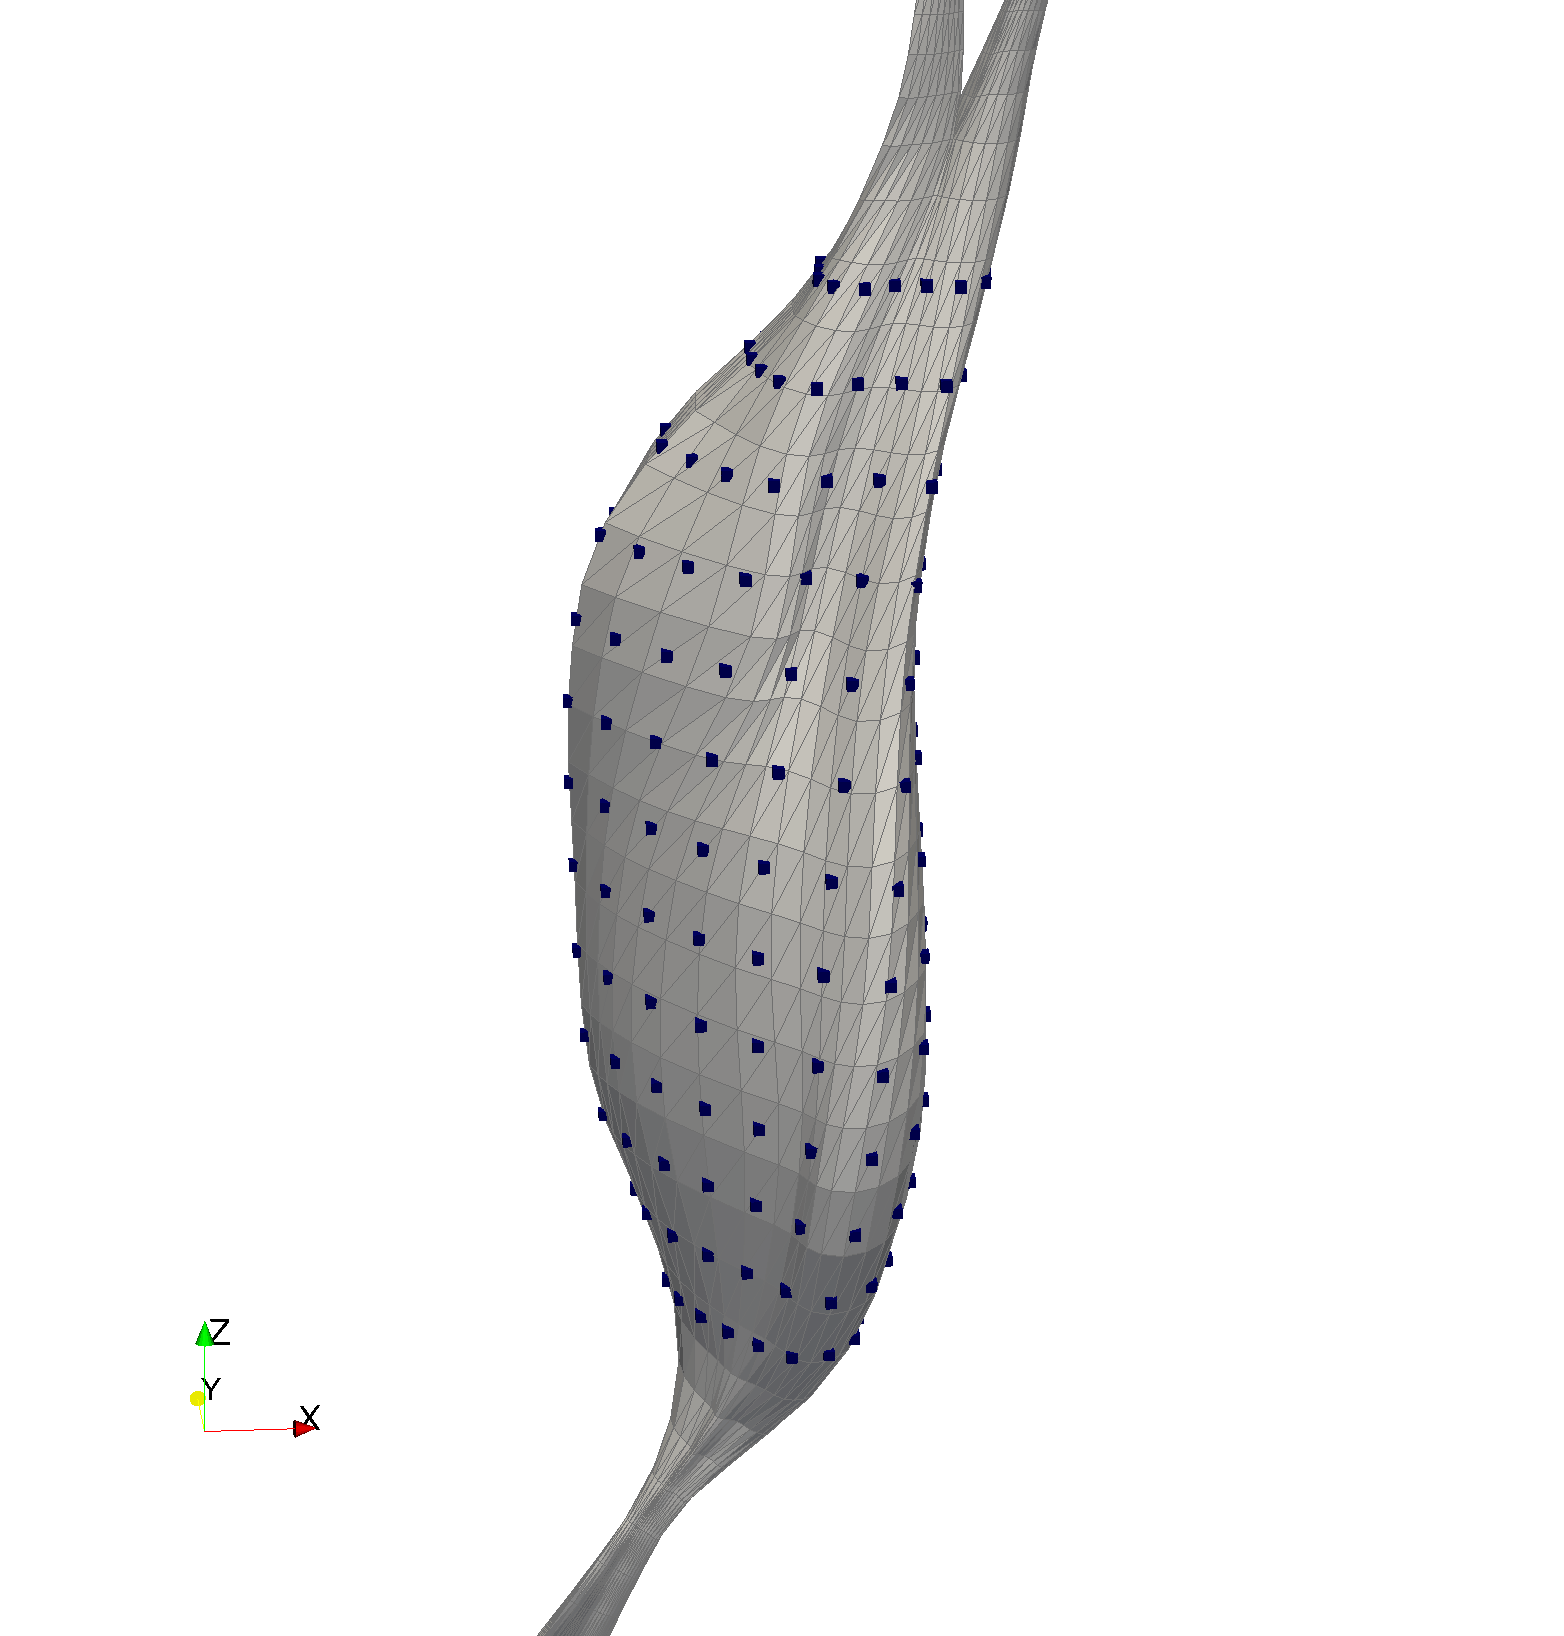
\includegraphics[height=9cm]{images/fiber_creation/serial_alg_0.png}% [trim=left bottom right top, clip]
    \caption{Extracted boundary points (blue) on the biceps surface mesh (gray). This is the result of line \ref{alg:1.1} in \cref{alg:serial_algorithm_1}.}%
    \label{fig:serial_alg_0}%
  \end{subfigure}
  \quad
  \begin{subfigure}[t]{0.51\textwidth}%
    \centering%
    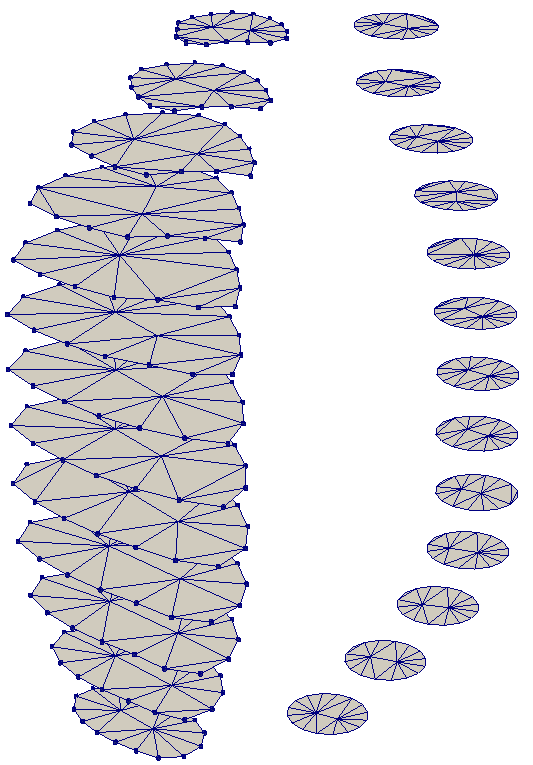
\includegraphics[height=9cm]{images/fiber_creation/serial_alg_3.png}%
    \caption{The generated triangulation of the slices (left) and the image $\bfy(\bfx)$ of the triangulation under the harmonic map (right). This figure shows the result of lines \ref{alg:1.2} and \ref{alg:1.3} in \cref{alg:serial_algorithm_1}.}%
    \label{fig:serial_alg_3}%
  \end{subfigure}\\
  \centering%
  \begin{subfigure}[t]{0.49\textwidth}%
    \centering%
    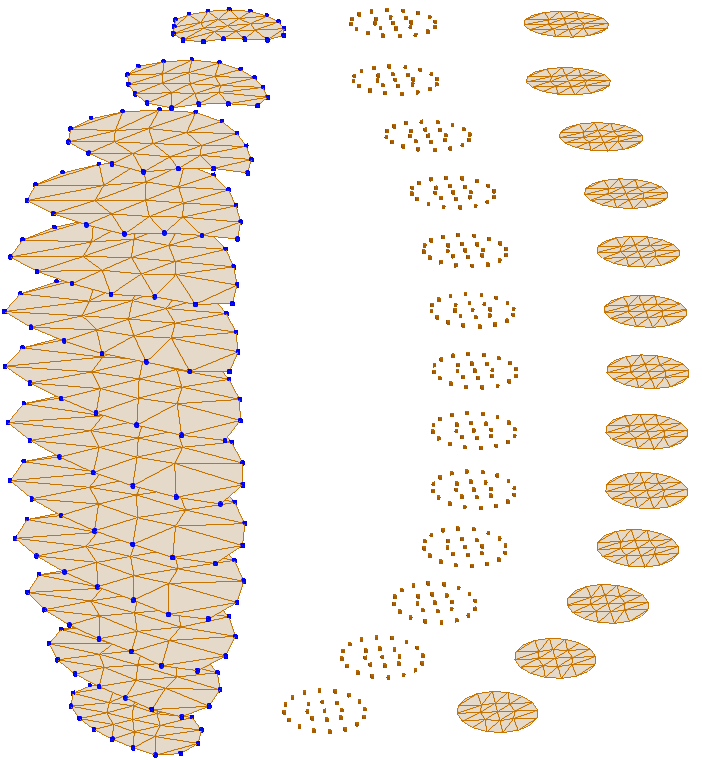
\includegraphics[height=9cm]{images/fiber_creation/serial_alg_4_orange.png}%
    \caption{Grid in parameter space (right) and muscle domain (left), result after line \ref{alg:1.4} in \cref{alg:serial_algorithm_1}.}%
    \label{fig:serial_alg_4}%
  \end{subfigure}
  \hfill{}
  \begin{subfigure}[t]{0.4\textwidth}%
    \centering%
    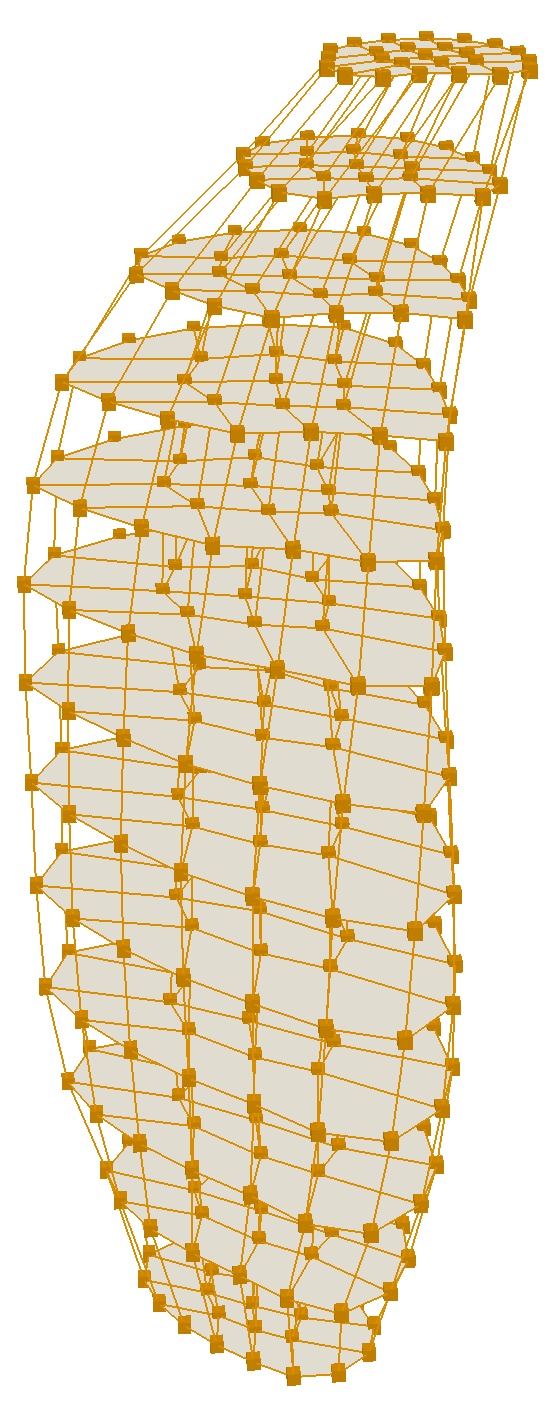
\includegraphics[height=9cm]{images/fiber_creation/serial_alg_8_orange.png}%
    \caption{3D elements formed by connecting the slices in line \ref{1.5} in \cref{alg:serial_algorithm_1}.}%
    \label{fig:serial_alg_8}%
  \end{subfigure}
  \caption{Steps of the serial algorithm for 3D mesh generation, \cref{alg:serial_algorithm_1}, executed directly on the surface mesh of the biceps muscle (not the B-spline surface).}%
  \label{fig:serial_alg}%
\end{figure}%
%

\subsection{Triangulation of the Slices}\label{sec:triangulation_of_the_slices}
The points of each ring enclose a planar, polygonal surface, a \emph{slice} $S_M$ of the muscle.
The next step in the algorithm, line \ref{alg:1.2}, is to triangulate the extracted slices, i.e., to construct triangles that decompose the polygons. The result of this step is visualized on the left side in \cref{fig:serial_alg_3}.

We select three different methods to construct this triangulation. The first and second methods are based on Delaunay triangulations. The third method creates a custom triangulation using a simple construction scheme with only one additional point.
\Cref{fig:triangulations} visualizes results of the three methods for one slice.

The first method uses the tessellation algorithm from the spatial algorithms and data structures module of the Python package \emph{SciPy}. 
The Quickhull algorithm \cite{quickhull} is used which triangulates the convex hull of the points. In consequence, the triangulations of concave slices have triangles that lie outside the interior of the slice, which is a disadvantage. An advantage is that the triangulation uses all given points and no new points are added. However, this often results in meshes of lower quality than if adding additional points were allowed.
The example in \cref{fig:triangulation_0} shows such a concave slice. At the bottom of the domain, the triangles are outside the slice and almost degenerate.

The second method uses a Delaunay refinement algorithm described in \cite{Delaunay2002} and implementated in the \emph{Triangle} software \cite{shewchuk96b}. A conforming, constrained Delaunay triangulation is created. The triangulation correctly handles convex and concave domains.
Conforming means that the triangulation uses the given points at the boundary. Additional points on the boundary as well as in the interior are added. The triangulation is constraint to generate triangles with minimum angles of 20 degrees and a maximum area $A$ that is set to a value depending on the area of the bounding box. In consequence, the generated triangulations of all slices have a guaranteed mesh quality in terms of angles and about the same size and number of triangles.

Comparing the result of the second method in \cref{fig:triangulation_1} with the result of the first method in \cref{fig:triangulation_0} shows the better triangulation quality as the triangles all have larger angles.

The third method places one additional point at the center of gravity of the given points. Triangles are constructed by connecting the center point with two adjacent points on the boundary, for all given points. The resulting triangulation resembles a pie chart. For some extreme concave slices, this method also creates triangles that partly lie outside the slice, but this occurs rarely with muscle cross-sections. The advantage of this approach is its simplicity.
\Cref{fig:triangulation_2} shows the result for an exemplary slice. In contrast to the first method, the third method creates a valid triangulation despite the concave domain.

\begin{figure}%
  \centering%
  \begin{subfigure}[t]{0.31\textwidth}%
    \centering%
    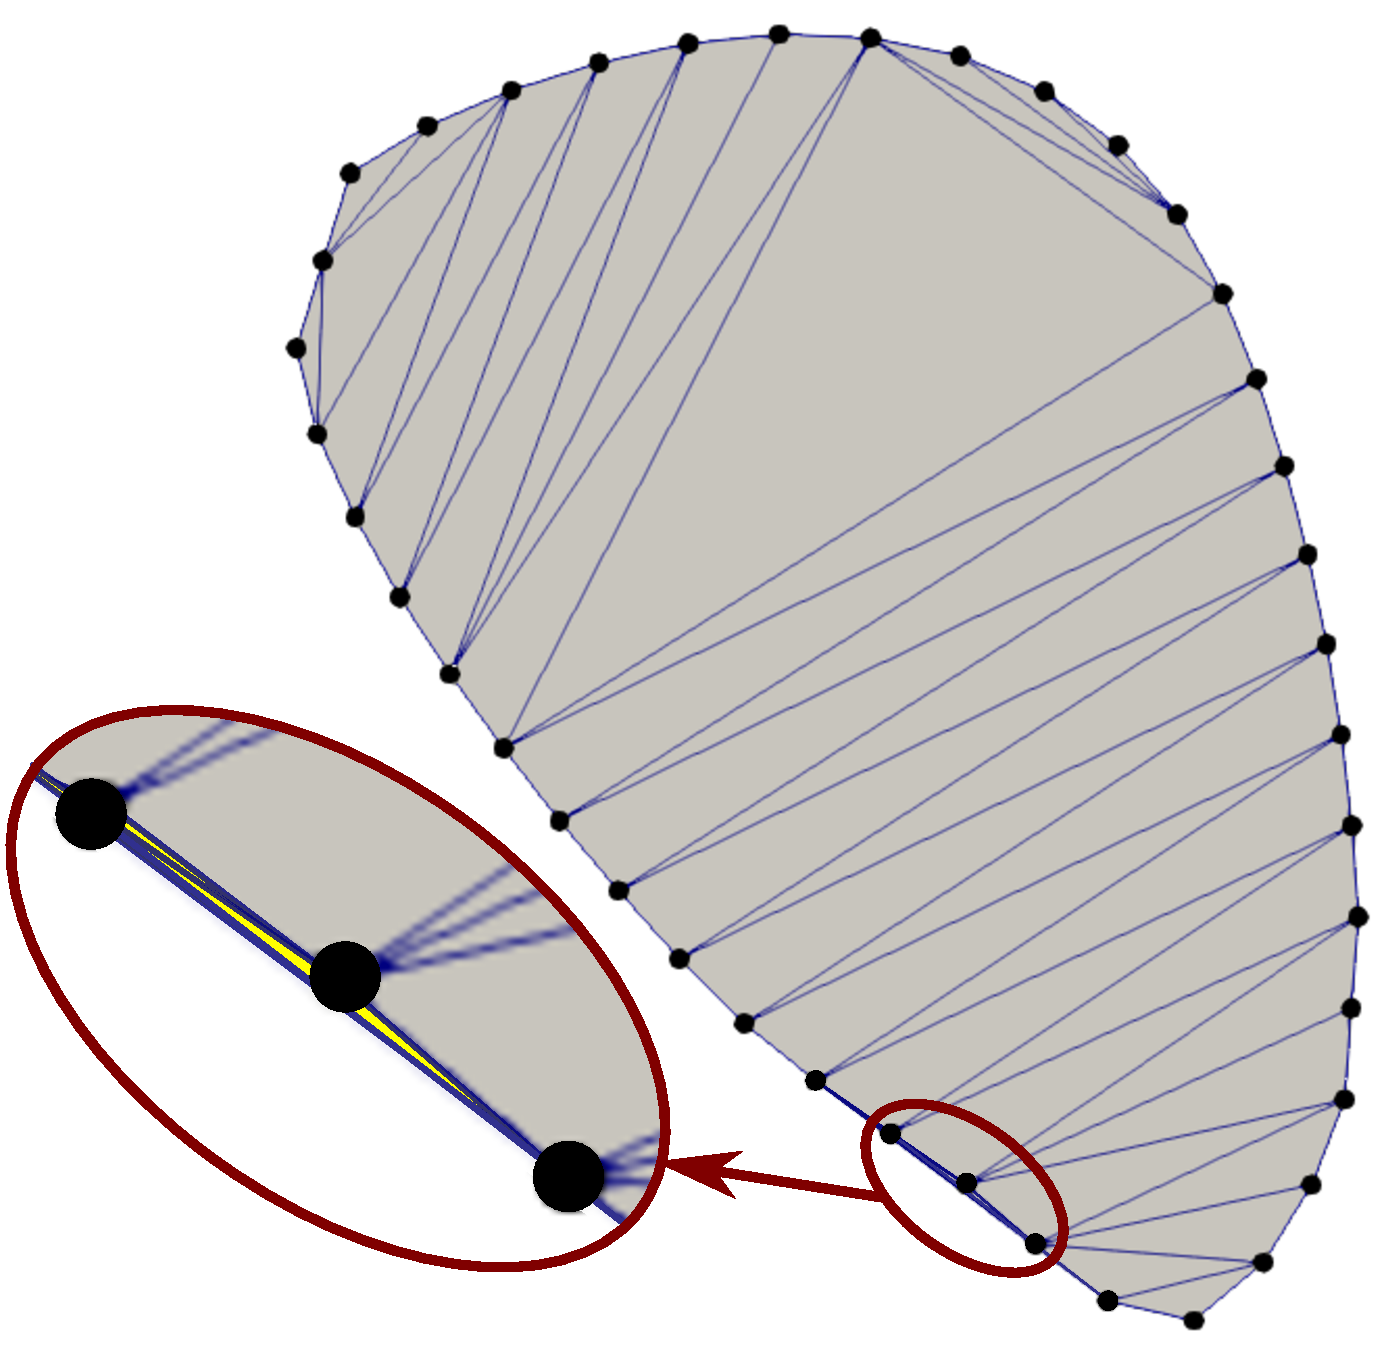
\includegraphics[height=55mm]{images/fiber_creation/triangulation_0.pdf}%
    \caption{First triangulation method}%
    \label{fig:triangulation_0}%
  \end{subfigure}
  \qquad
  \begin{subfigure}[t]{0.27\textwidth}%
    \centering%
    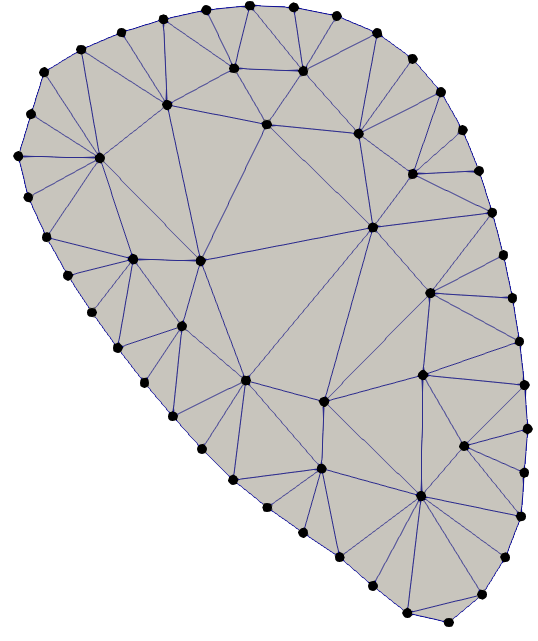
\includegraphics[height=55mm]{images/fiber_creation/triangulation_1.png}%
    \caption{Second trian\-gulation method}%
    \label{fig:triangulation_1}%
  \end{subfigure}
  \quad
  \begin{subfigure}[t]{0.32\textwidth}%
    \centering%
    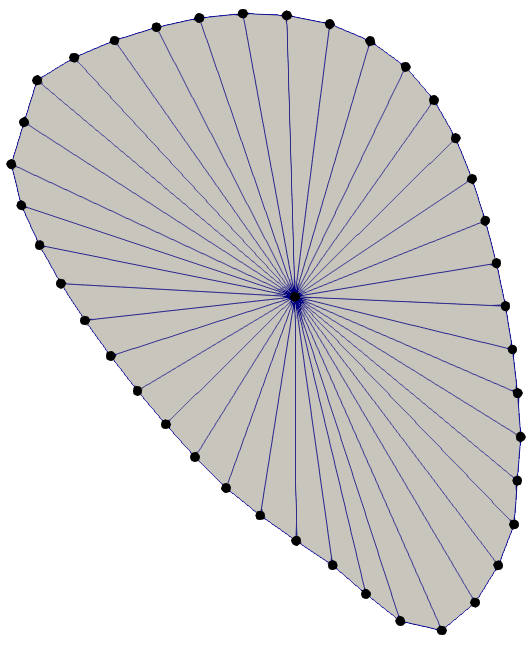
\includegraphics[height=55mm]{images/fiber_creation/triangulation_2.png}%
    \caption{Third triangulation method}%
    \label{fig:triangulation_2}%
  \end{subfigure}
  \caption{Intermediate step of 3D mesh generation: triangulation of slices, result of different triangulation methods for a slice in the center of the biceps muscle.}%
  \label{fig:triangulations}%
\end{figure}%

\subsection{Harmonic Maps}

Next, harmonic maps are created that allow to smoothly map a given 2D reference mesh onto an actual cross-section of the muscle. The initial application of harmonic maps to meshes used for biomedical simulations is given by \cite{marchandise2010quality} and \cite{Marchandise2_2011}. The authors improve a given, oversampled surface mesh obtained from classical segmentation. This is done by partitioning the surface into multiple mesh partitions of zero genus (i.e., containing no holes) and transforming them to a reference space using harmonic maps. There, controlled remeshing is carried out before the transformation is reversed.

In our algorithm, harmonic maps are also used for the purpose of generating high quality meshes. In contrast to the literature, the mapping is based on the muscle slices instead of the surface. Also, different parameter domains are investigated.

A function $u: \Omega \to \R$ on a domain $\Omega \in \R^d$ is \emph{harmonic} if it is a solution of the Laplace equation $Δu = 0$.
From variational calculus, it is known that harmonic functions are extremals of the \emph{Dirichlet energy functional} \cite{weyl1940},
\begin{align*}
  E[u] = \dfrac12 \int_\Omega |\nabla u|^2 \,\d\bfx.
\end{align*}
For an intuitive understanding, the map $u$ can be seen as deforming an elastic material that is initially located tension-free in the domain $\Omega$.
Then, the Dirichlet energy $E[u]$ describes the total amount of squared stretch or elastic energy resulting from the tension that occurs in the deformed state. A harmonic map minimizes this total tension. Qualitatively, the map deforms neighborhoods of all points in $\Omega$ by a similar amount, thus, preserving geometrical structures in $\Omega$, e.g., given by a mesh. The idea of our approach is that 
applying a harmonic map on a mesh with good quality preserves the mesh quality also in the image under the map.

In \cref{alg:serial_algorithm_1}, computing the harmonic maps $u$ and $v$ is done in line \ref{alg:1.3}. For a given slice $S_M$, the functions $u$ and $v$ map from points $\bfx \in S_M$ to coordinates $u(\bfx),v(\bfx)\in \R$ of a parameter domain $\Omega_P \subset \R^2$. The parameter domain is either a unit circle or a unit square.

The vector $\bfy(\bfx) := (u(\bfx), v(\bfx))^\top$ for $\bfx \in S_M$ is interpreted as position in $\Omega_P$. The maps are constructed such that the boundary $∂S_M$ of the slice $S_M$ is mapped to the boundary $∂\Omega_P$ of the parameter domain $\Omega_P$ while preserving the distance between points on the boundary.
The mapping $\bfy: S_M \to \Omega_P$ is bijective and harmonic, i.e., the Laplacians of $u$ and $v$ are zero.
More specifically, $u : S_M \to \R$ and $v : S_M \to \R$ are solutions of
%
\begin{equation}\label{eq:def_harmonic_maps}
  \begin{array}{l}
    Δu(\bfx) = 0, \quad Δv(\bfx) = 0 \quad \forall \bfx \in S_M.
  \end{array}
\end{equation}
%
To derive suitable Dirichlet boundary conditions for these equations, we consider a uniform parametrization $\bfp:[0,1] \to ∂S_M$ of the boundary $∂S_M$ of the slice, i.e., 
%
\begin{align*}
  \p{l(t)}{t} = c \in \R \quad \forall t \in [0,1], \quad \text{where } l(t) := \i{0}{t} |\bfp'(\tau)| \,\d\tau.
\end{align*}
%
We require the image of the boundary parametrization in $\Omega_P$ to be also uniform, i.e.,%
\begin{align*}
  \p{l_P(t)}{t} = c_P \in \R \quad \forall t \in [0,1], \quad \text{where } l_P(t) := \i{0}{t} |\bfy'\big(\bfp(\tau\big)| \,\d\tau.
\end{align*}
%
Corresponding boundary points $\bfx_\text{M,boundary} \in S_M$ and $\bfx_\text{P,boundary} = (u_\text{P,boundary},v_\text{P,boundary})^\top$ can be defined. This leads to the following Dirichlet boundary conditions that close the definition in \cref{eq:def_harmonic_maps}:%
\begin{align}\label{eq:bc_harmonic_maps}
  u(\bfx_\text{M,boundary}) = u_\text{P,boundary}, \quad v(\bfx_\text{M,boundary}) = v_\text{P,boundary}.
\end{align}
%

Equations \eqref{eq:def_harmonic_maps} and \eqref{eq:bc_harmonic_maps} describe a boundary value problem of ordinary differential equations for $u$ and $v$. We solve it using the Finite Element Method and the spatial discretization given by the triangulation of the slices.
Depending on the method of triangulation, a different number of degrees of freedom is given. For the first method with the Quickhull algorithm, no degree of freedom is present and no system of equations needs to be solved. Then, the mapping is only a FE interpolation of the boundary mapping.
For the third method, only one degree of freedom for the center point needs to be computed. The second method has as many degrees of freedom as there are additional points inserted during the Delaunay refinement.

The first step is to compute the prescribed boundary points $\bfx_\text{P,boundary}$ in parameter space. When using the first and third triangulation methods, the boundary points on the slices are  equidistant and therefore the same number of points need to be sampled equidistantly on the boundary $∂\Omega_P$ of the parameter space.
If the second triangulation method, which potentially adds additional points is used, the same number of points  are created on the boundary $∂\Omega_P$ of the slice as are given on the slice $∂S_M$. The boundary points are created such that the relations of their distances are the same on $∂\Omega_P$ as for the original points on $∂S_M$.

Using the standard procedure of the Finite Element method for $Δu(\bfx) = 0$ on $S_M$ and $u=f(\bfx)$ on $∂S_M$, e.g., as outlined in \cite{Remacle2010}, leads to the weak form with ansatz and test functions $\phi$,
\begin{align}\label{eq:est_fe_w}
    \i{S_M}{} (\nabla u^\top \nabla \phi + \nabla f(\bfx)^\top \nabla \phi) \,\d \bfx = 0 \quad \forall \phi \in \mathcal{H}_0^1.
\end{align}
Standard linear hat functions are used on the triangles, such that they provide the interpolation property $\phi_i(\bfx_j) = \delta_{ij}$. Using the barycentric parametrization of triangles with points $\bfp^1,\bfp^2$ and $\bfp^3$ introduced in \cref{eq:barycentric_triangle}, we define the ansatz functions and get their derivatives within the elements by:
%
\begin{align*}
  \phi^{(e)}_1 &= (1 - \xi_1)(1 - \xi_2), \quad&
  \phi^{(e)}_2 &= \xi_1 (1 - \xi_2), \quad &
  \phi^{(e)}_3 &= (1 - \xi_1) \xi_2,\\[4mm]
  \nabla \phi^{(e)}_1 &= (\xi_2-1, \xi_1 - 1)^\top, \quad&
  \nabla \phi^{(e)}_2 &= (1-\xi_2, -\xi_1)^\top, \quad&
  \nabla \phi^{(e)}_3 &= (-\xi_2, 1-\xi_1)^\top.
\end{align*}
The superscript $\square^{(e)}$ refers to the definition of the functions within elements. The global assembly involves composing the global nodal functions $\phi_i(\bfx)$ for nodes indexed by $i=1, \dots, n_\text{nodes}$ and using a mapping between the barycentric coordinates $\xi_1,\xi_2 \in [0,1]^2$ inside the elements to the global coordinates $\bfx \in S_M$.
Inserting the discretization
\begin{align*}
  u_h(\bfx) = \s{i=1}{n_\text{nodes}} u_i\,\phi_i(\xi_1(\bfx), \xi_2(\bfx))
\end{align*}
into \cref{eq:est_fe_w} leads to the form
\begin{equation}\label{eq:est_weak_form}
  \begin{array}{lll}
    \s{i=1}{n_\text{nodes}}u_i \i{S_M}{} \nabla_\bfx \phi_i^\top \nabla_\bfx \phi_j \,\d\bfx + \s{i=1}{n_\text{nodes}} f_i \i{S_M}{} \nabla_\bfx \phi_i^\top \nabla_\bfx \phi_j \,\d \bfx = 0\,\quad \forall j=1,\dots,n_\text{nodes}.
  \end{array}
\end{equation}
The integrations are executed element-wise and over the elemental coordinates $\xi_1,\xi_2$. 
The transformation to elemental coordinates involves the computation of the Jacobian $J=\d\bfx/\d\bfxi$ of the mapping between element coordinates $\bfxi = (ξ_1,ξ_2)$ and global coordinates $\bfx$. From the definition in \cref{eq:barycentric_triangle}, it follows that
\begin{align*}
  J = \d{\bfx}{\bfxi} = [\bfp^2-\bfp^1, \bfp^3-\bfp^1].\\[4mm]
\end{align*}
The metric tensor for this mapping is given by
\begin{align*}
  \mathcal{M} := \left(\d{x}{\bfxi}\right)^T \left(\d{x}{\bfxi}\right).
\end{align*}
%
The transformation of the integrals in \cref{eq:est_weak_form} introduces an additional integration factor $\sqrt{\det{\mathcal{M}}}$.
We get the following matrix equation:
\begin{align}\label{eq:est_fe_system}
  M_u \bfu = -M_f\,\bff,
\end{align}
with the vector $\bfu$ of nodal solution values, the vector $\bff$ of nodal Dirichlet boundary condition values at the boundary and the global stiffness matrices $M_u$ and $M_f$. The two global stiffness matrices are assembled from the element stiffness matrices $M^\text{(e)}$ for the degrees of freedom at all nodes respectively at the boundary nodes. The entries of the element stiffness matrices are given by
\begin{align*}
  M^\text{(e)}_{i,j} = \i{0}{1}\i{0}{1-\xi_1}   \nabla \phi_i^{(e)}(\xi_1,\xi_2)^\top \, \mathcal{M}^{-1} \, \nabla \phi_j^{(e)}(\xi_1,\xi_2) \, \sqrt{\det{\mathcal{M}}}  \,\d\xi_2\d\xi_1.
\end{align*}

By solving \cref{eq:est_fe_system} for $\bfu$, we get the discretized harmonic map $u$.
The Finite Element formulation and computation for $v$ is analogous and uses the same global stiffness matrices.

\Cref{fig:harmonic_map_solution} visualizes the triangulation of $S_M$ and the solutions $u(\bfx)$ and $v(\bfx)$ for a circular parameter domain $\Omega_P$ and an exemplary muscle slice in the first two plots. The color range from bright yellow to dark violet corresponds to increasing values of $u$ and $v$. It can be seen that the $u$ values increase from left to right whereas the $v$ values increase from bottom to top, corresponding to the horizontal and vertical coordinate axes $y_1$ and $y_2$ of $\Omega_P$.


Applying the computed harmonic map $\bfy(\bfx)$ to the triangulation of the slices results in a triangulation of the parameter domain $\Omega_P$. This is shown in the third plot of \cref{fig:harmonic_map_solution} and in \cref{fig:serial_alg_3}.
In both figures, the triangulation of the slices was generated using the second triangulation method with the constrained Delaunay triangulation. On the right side of \cref{fig:serial_alg_3}, the image $\bfy(\bfx)$ under the harmonic map of the triangulation in the slices is shown on the unit circle parameter domain.

\begin{figure}%
  \centering%
  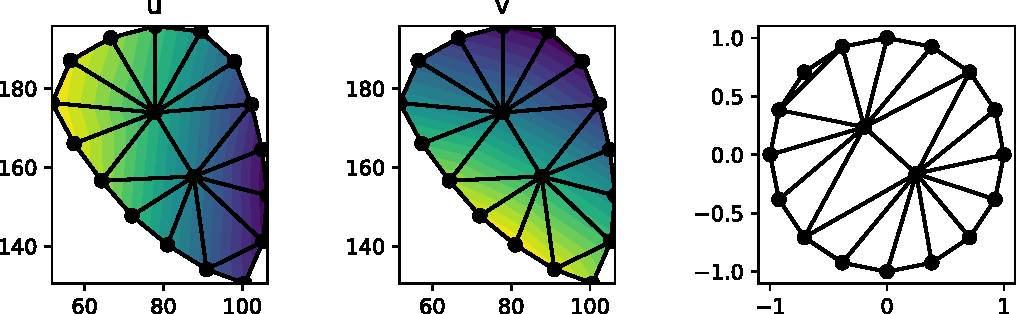
\includegraphics[width=\textwidth]{images/fiber_creation/harmonic_map_9b.pdf}%
  \caption{Quality improvement of muscle slice meshes as a basis for 3D mesh generation: Initial triangulations and harmonic map for a slice $S_M$ of the biceps muscle. The first two plots show the solutions of $u$ and $v$ on the slice $S_M$. The third plot shows the image in $\Omega_P$ of the triangulation in $S_M$ under the harmonic map.}%
  \label{fig:harmonic_map_solution}%
\end{figure}%

\subsection{Construction of a Regular Grid in the Parameter Domain}
The next step in \cref{alg:serial_algorithm_1} is the construction of a 2D structured, regular grid in the parameter domain $\Omega_P$, as stated in line \ref{alg:1.4}. This grid will then be mapped to the slices $S_M$. Creating a structured grid of quadrilateral elements in a given domain is also called \emph{quadrangulation}.

The parameter domain $\Omega_P$ can be selected to be either a unit square or a unit circle. For both choices, two different schemes how to generate a grid with a given number of cells can be selected.
\Cref{fig:quads} shows all four possiblities.

The first scheme, \cref{fig:quad_1}, uses an equidistant regular grid in a unit square. This is the easiest possibility to generate a quadrangulated reference domain. A possible issue is induced by the corners of the square. The grid will be mapped to a cross section of the muscle which has no sharp corners. Therefore, the cells of the grid will be distorted at the images of the corners, usually shortening diagonals that point towards the corners and lengthening the other diagonals. This assumption motivates the second scheme in \cref{fig:quad_2}. Here, the elements are already distorted in the described manner, with increasing distortion closer to the corners. The rationale is that the mapped cells in $S_M$ will then be less distorted.

We construct our second quadrangulation scheme of the unit square as follows. The diagonals of the square divide the domain into bottom, top, left and right quarters, which are considered separately.
For example, the bottom quarter is the triangle that is formed by the corner points $(0,0), (1,0)$ and the center point $(\frac12,\frac12)$ of the square. In the bottom quarter, the horizontal $x$ coordinate of a point $(x,y)$ in a uniform grid can be described by $x = \frac12 + \textrm{tan}(\phi)\,(\frac12-y)$ where $\phi$ is the angle between a line through $(x,y)$ and the center point $(\frac12,\frac12)$ and the $y$-axis. The points of the adjusted grid in the quadrangulation scheme are constructed by altering the value of $\phi$.
On every horizontal series of points in the bottom quarter, $\phi$ is varied linearly in $[-\pi/4,\pi/4]$ instead of the nonlinear progression according to the actual angle. This leads to the larger spacing between points near the diagonals. All four quarters are treated analogously to produce the shown symmetric pattern.

A different approach is to use a unit circle, which has no corners and therefore might resemble a muscle cross section more consistently. The first scheme of the unit circle is given in \cref{fig:quad_0}. It uses the radial and circumferential directions for the two dimensions of the grid. A disadvantage of this scheme is that the quadrilaterals at the center are degenerated to triangles. Additionally, the area of the cells varies significantly and the outer cells have unequal side lengths. 

To remedy this problem, we develop the second scheme given in \cref{fig:quad_3}. When traversing from the outer boundary towards the center point and considering the circumferential lines of grid points, the circle morphs into a square as the number of grid points decreases. This approach has the disadvantage that some cells have an inner angle of nearly \SI{180}{\degree}, especially four elements at the boundary. Apart from that, all elements have similar sized sides and angles.
The construction of this scheme is similar to the approach of scheme 2 on the unit square in that the domain is also divided into four quarters. However, different formulas for the point coordinates $(x,y)$ depending on the angle $\phi$ are used.
The detailed construction formulas of all four presented quadrangulation schemes are provided by their implementation in the code. The script \code{plot_quadrangulation_schemes.py} constructs and visualizes the four schemes with a configurable number of grid points.


Each construction scheme allows to specify the (squared) number of nodes and in consequence the number of cells. The examples in \cref{fig:quad_1,fig:quad_2,fig:quad_3} have $11 \times 11$ nodes and $10 \times 10$ cells. For \cref{fig:quad_0}, the numbers are slightly different. There are $10 \times (11 + 1)$ nodes resulting in $10 \times 11$ cells.

\begin{figure}%
  \centering%
  \begin{subfigure}[t]{0.48\textwidth}%
    \centering%
    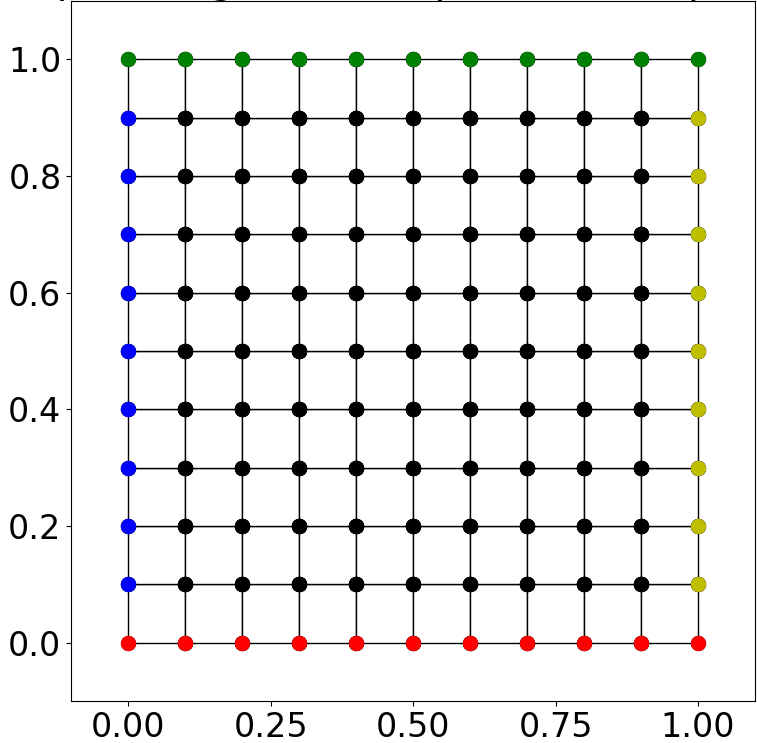
\includegraphics[width=\textwidth]{images/fiber_creation/quad_1.png}%
    \caption{Unit square, scheme 1}%
    \label{fig:quad_1}%
  \end{subfigure}
  \quad
  \begin{subfigure}[t]{0.48\textwidth}%
    \centering%
    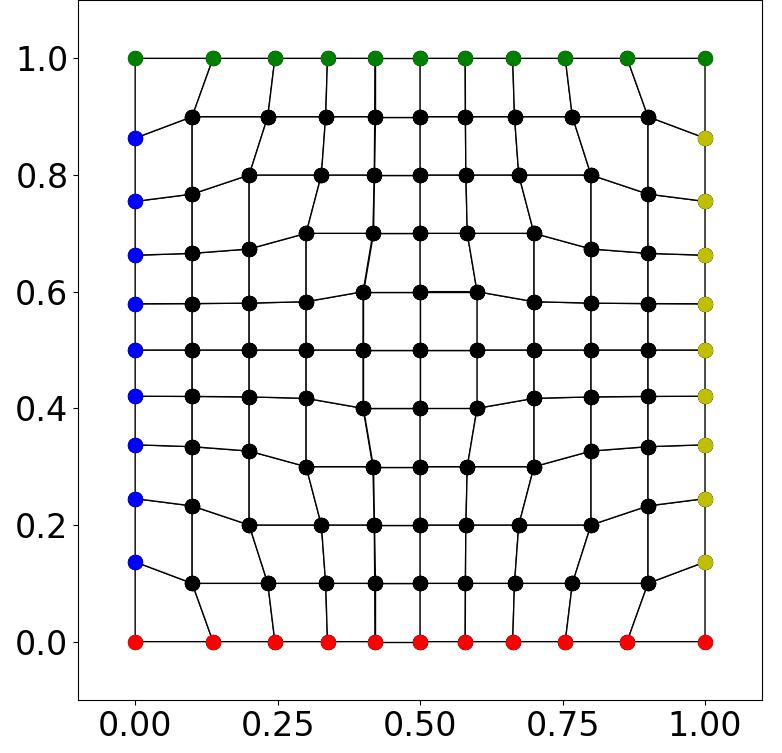
\includegraphics[width=\textwidth]{images/fiber_creation/quad_2.png}%
    \caption{Unit square, scheme 2}%
    \label{fig:quad_2}%
  \end{subfigure}
  \begin{subfigure}[t]{0.48\textwidth}%
    \centering%
    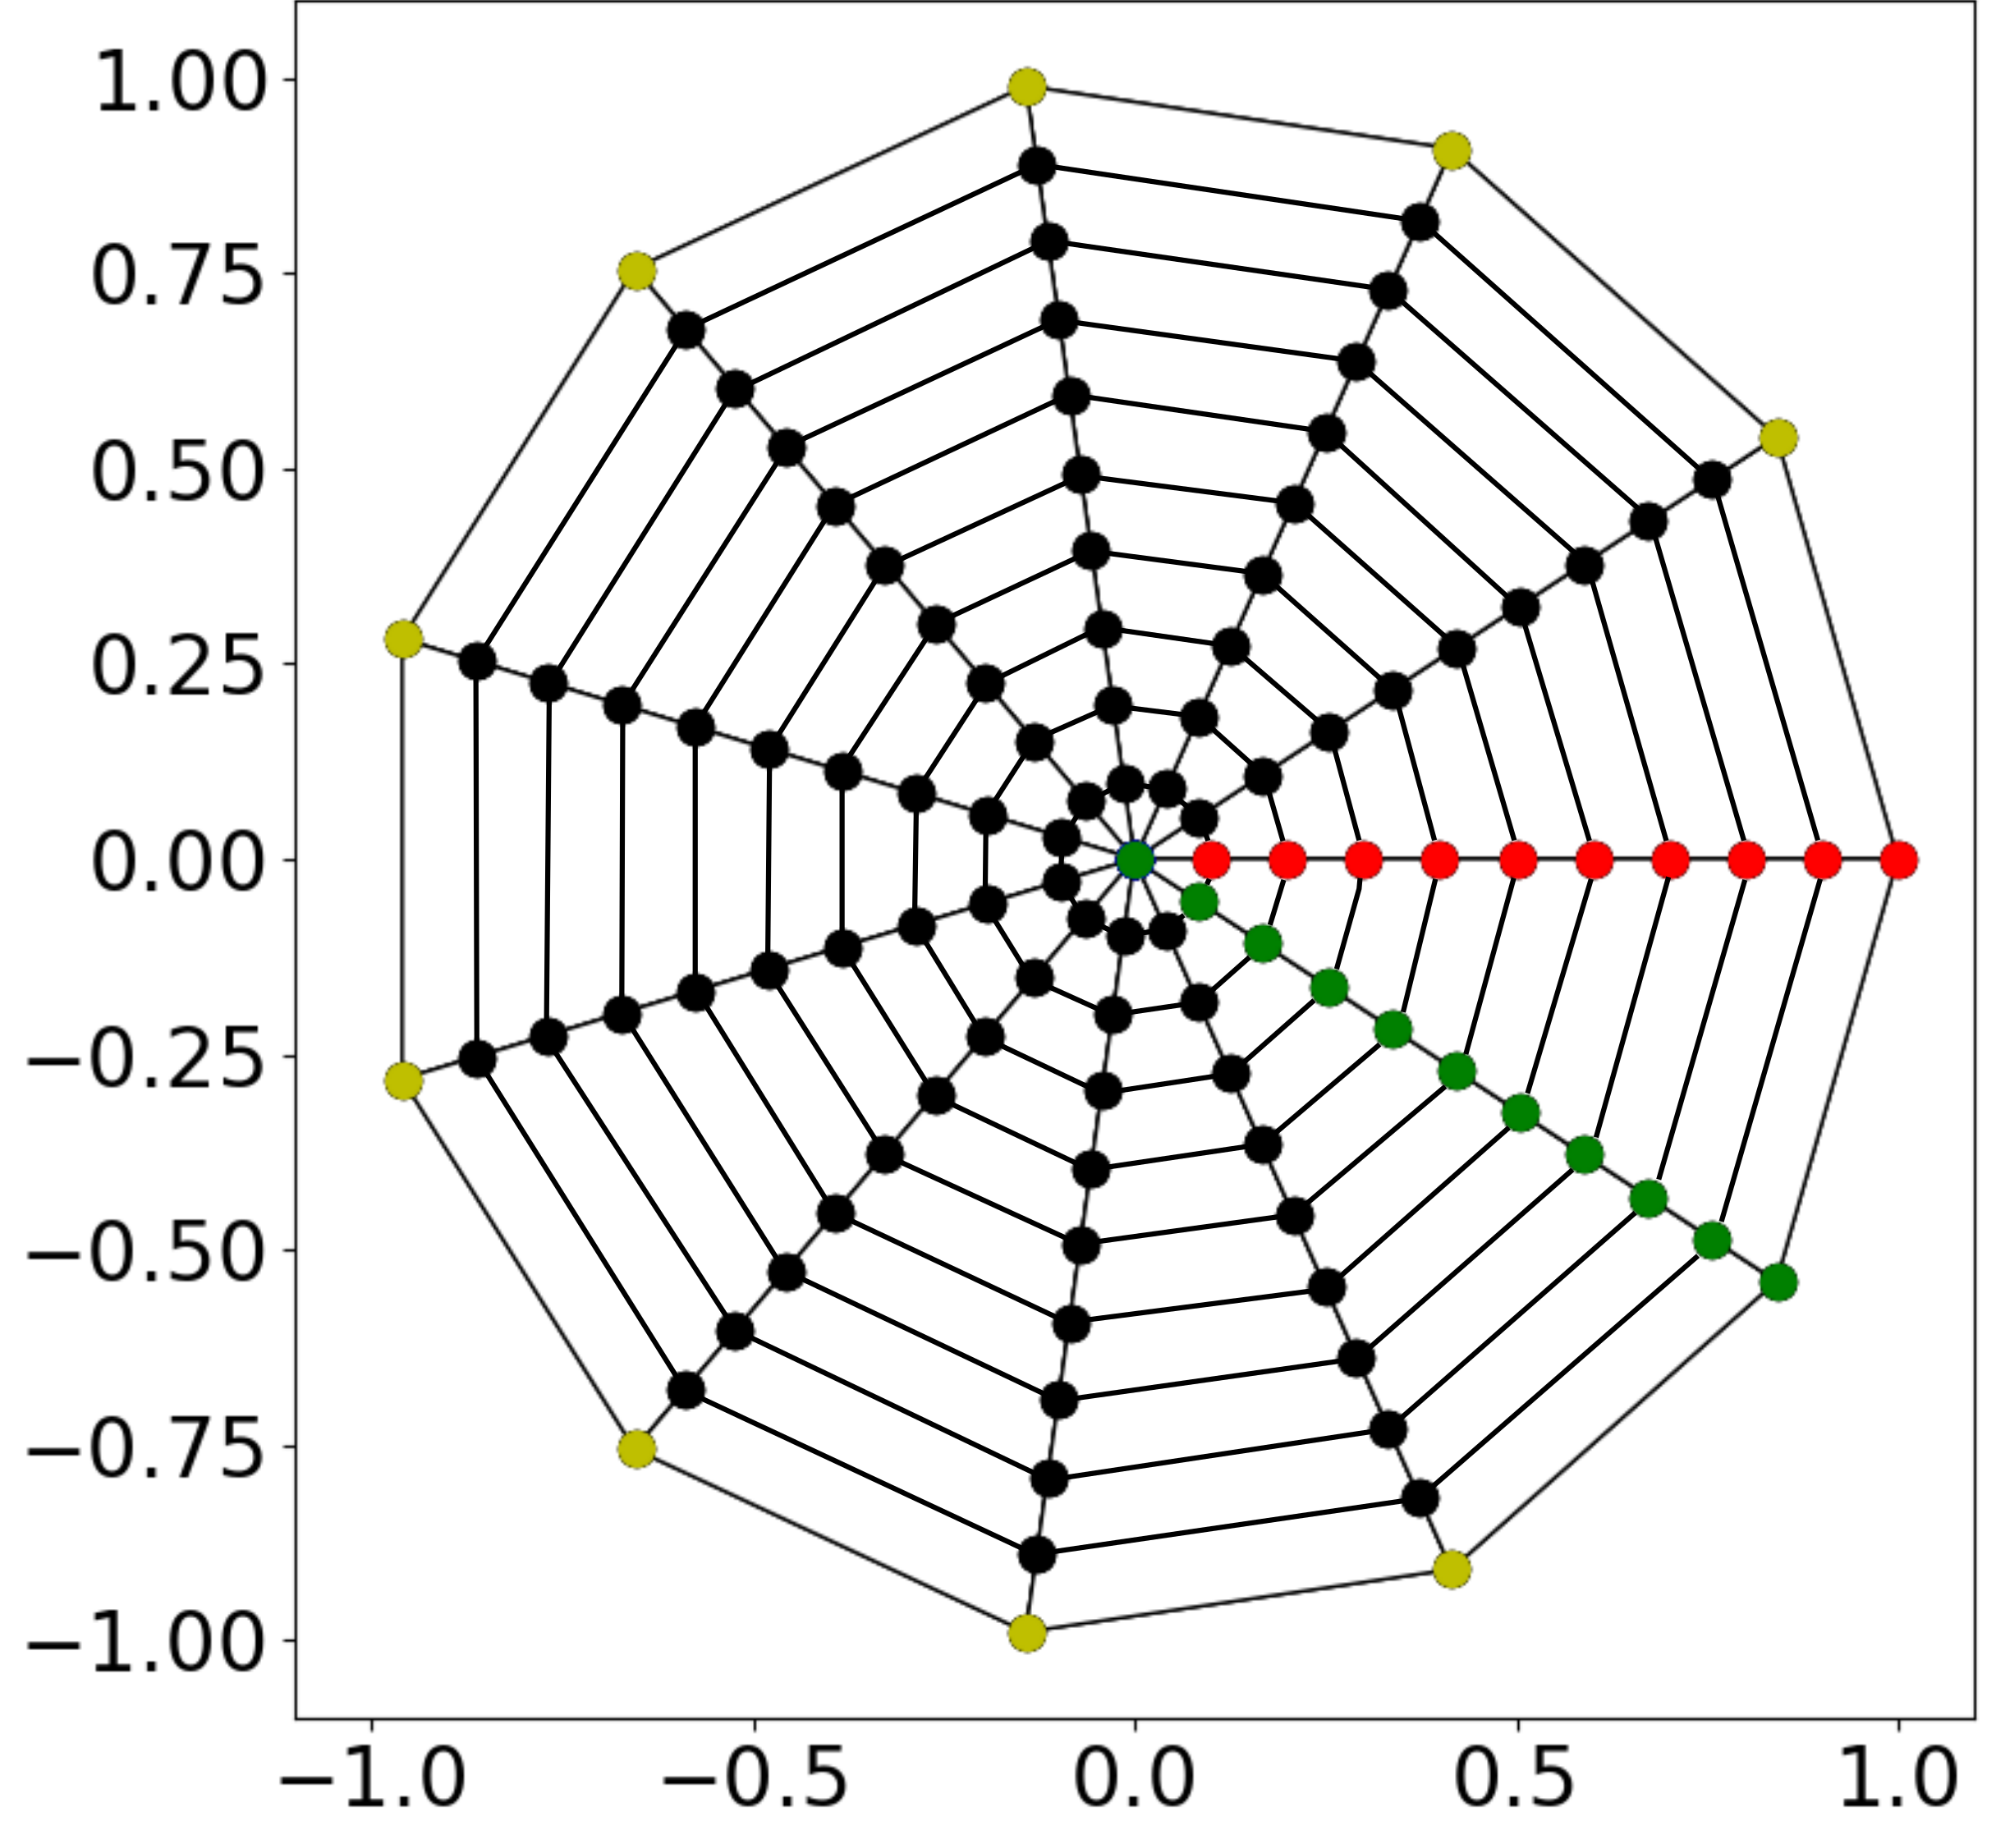
\includegraphics[width=\textwidth]{images/fiber_creation/quad_0.png}%
    \caption{Unit circle, scheme 1}%
    \label{fig:quad_0}%
  \end{subfigure}
  \quad
  \begin{subfigure}[t]{0.48\textwidth}%
    \centering%
    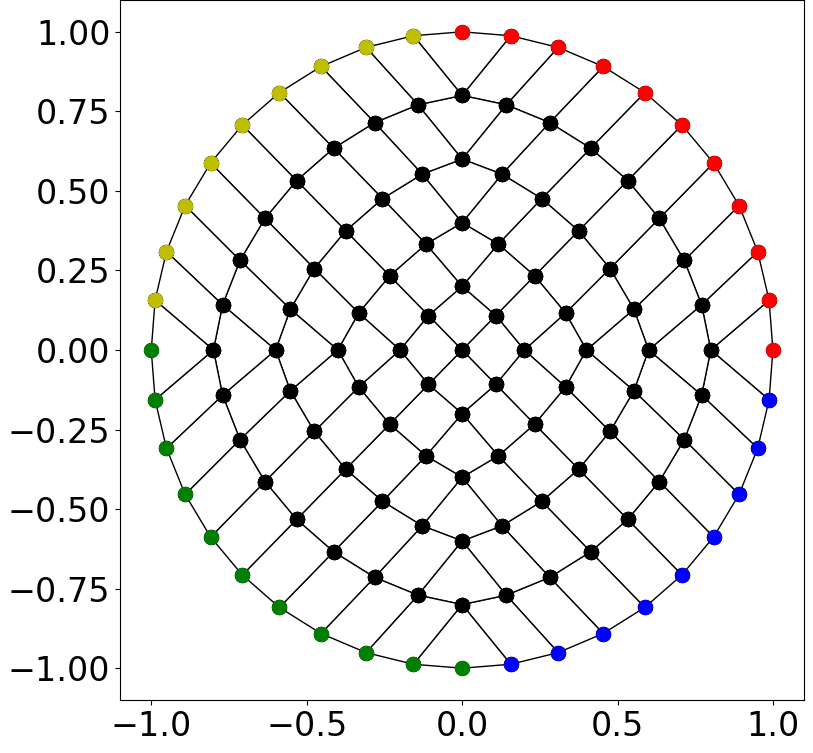
\includegraphics[width=\textwidth]{images/fiber_creation/quad_3.png}%
    \caption{Unit circle, scheme 2}%
    \label{fig:quad_3}%
  \end{subfigure}
  \caption{Four different quadrangulation schemes of the parameter domain with $11\times 11$ nodes. The boundaries of the grid are colored for better perceptiblity. In (a) and (b), the parameter domain is a unit square with a uniform grid (a) and an adjusted grid (b) that tries to reduce the problem of degenerate elements at the corners of the muscle slices. In (c) and (d), quadrangulations on a unit circle parameter domain are shown. (c) shows a rotationally symmetric construction scheme whereas the approach in (d) is similar to a uniform grid.}%
  \label{fig:quads}%
\end{figure}%

Next, the grid in the parameter domain is transferred to the muscle domain by applying the harmonic map $\bfy(\bfx) \in S_M$ on every point of the quadrangulation $\bfx \in \Omega_P$. This is illustrated in \cref{fig:serial_alg_4} for a parameter domain consisting of the unit circle, with quadrangulation scheme 2 and $5 \times 5$ nodes. The cells of the grid in $\Omega_P$ are shown in the right-most stack of domains. The grid points are visualized left of the grids. The resulting image of the mesh in the slices $S_M$ is shown on the left. For visualization reasons, each quadrilateral has been split into two triangles.

\subsection{Formation of Three-Dimensional Elements}

The result of the previous steps is a number of quadrangulated muscle slices. The grid on every slice has the same number of nodes and elements. The nodes on the boundary of neighboring slices are positioned similarly.

The final step of \cref{alg:serial_algorithm_1} is line \ref{alg:1.5}, the formation of 3D elements. Inserting vertical edges between all corresponding nodes on two neighboring slices creates a set of 3D hexahedral elements and, thus, an overall 3D hexahedral mesh of the muscle volume. This step is visualized in \cref{fig:serial_alg_8}.

\subsection{Generation of Fiber Meshes}\label{sec:generation_of_fiber_meshes}

1D fiber meshes are created following the approach of computing a divergence free vector field introduced in \cite{Choi2013}. The steps are given in \cref{alg:serial_algorithm_2}.

The Laplace problem to be solved can be stated as%
\begin{align}\label{eq:fiberest_laplace}
  Δp(\bfx) = 0 \quad \text{for } \bfx \in \Omega_M.
\end{align}
The vector field is given by the gradient $\nabla p$ of a solution $p$ of \cref{eq:fiberest_laplace}. The quantities can be interpreted as pressure $p$ and (negative) velocity field $\nabla p$ of a steady flow.
The muscle fibers are given as streamlines or, equivalently, pathlines in this velocity field. Every streamline $\bfx : [-c_1,c_2] \subset \R \to \Omega_M$ with $c_1,c_2 > 0$ is defined by a seed point $\bfx_0$ and the property that it is tangent to the velocity field at any point:
\begin{align*}
  \bfx(0) = \bfx_0,\quad
  \p{\bfx(s)}{s} = \nabla p\big(\bfx(s)\big).
\end{align*}

As proposed by \cite{Choi2013}, Neumann boundary conditions can be specified for the bottom and top surfaces of the muscle volume, $∂\Omega_{M, \text{bottom}}$ and $∂\Omega_{M, \text{top}}$:
\begin{equation}\label{eq:fiberest_neumann}
\begin{array}{rlrlr}
  \d{p(\bfx)}{\bfx} \cdot \bfn &= F_\text{in}, \quad &&\text{for } \bfx \in ∂\Omega_{M, \text{bottom}},\\[4mm]
  \d{p(\bfx)}{\bfx} \cdot \bfn &= F_\text{out}, \quad &&\text{for } \bfx \in ∂\Omega_{M, \text{top}}.
\end{array}
\end{equation}
The in and outflow values $F_\text{in}<0$ and $F_\text{out}>0$ are balanced such that the total inflow ${F_\text{in}\cdot \mu(∂\Omega_{M, \text{bottom}})}$ compensates the total outflow ${F_\text{in}\cdot \mu(∂\Omega_{M, \text{bottom}})}$. Here, $\mu(∂\Omega)$ is the surface area of the respective boundary.

Alternatively, Dirichlet boundary conditions can be specified:
\begin{equation}\label{eq:fiberest_dirichlet}
\begin{array}{rlrlr}
  p(\bfx) &= 0, \quad &&\text{for } \bfx \in ∂\Omega_{M, \text{bottom}},\\[4mm]
  p(\bfx) &= 1, \quad &&\text{for } \bfx \in ∂\Omega_{M, \text{top}}.
\end{array}
\end{equation}
The specification of Dirichlet boundary conditions has the same effect as Neumann boundary conditions and is easier to define. The in and outflows are still orthogonal to the boundary because the prescribed value of $p$ does not vary in the planar boundary.

The boundary value problem given by \cref{eq:fiberest_laplace,eq:fiberest_neumann}  or \cref{eq:fiberest_laplace,eq:fiberest_dirichlet} is discretized by the Finite Element method with linear or quadratic ansatz functions and solved by our software \opendihu{} using the 3D mesh generated from \cref{alg:serial_algorithm_1}. The divergence free gradient field is visualized in \cref{fig:potential_flow}. The gradient values are directly given by the Finite Element discretization. The gradient is elementwise constant for linear ansatz functions and trilinear for quadratic ansatz functions.

The next step in \cref{alg:serial_algorithm_2} is line \ref{line:2.3}, tracing streamlines through the gradient field. Seed points are selected on the 2D cross-section at the vertical center of the 3D muscle domain. The seed points are sampled regularly on the square or circular parameter domain according to the quadrangulation scheme and then mapped to the respective muscle slice.
Because the 3D mesh was created using harmonic maps, the resulting spacing between the seed points is very uniform.

For the tracing of streamlines, the semi-analytical Pollock's method \cite{Pollock1988} is often used, which was originally developed for fixed 2D finite difference grids. Extensions to irregular 3D grids and for given velocities at nodes instead of fluxes over faces have been formulated \cite{HAEGLAND2007Streamline}. Other, more accurate algorithms exist \cite{cordes1992continuous}, including higher order formulations \cite{juanes2006unified}.

Because modeling muscle fascicles is only a heuristic approach, the generated streamlines do not have to be exceptionally accurate. Therefore, we use a fully numeric method. The streamlines are generated by explicit Euler integration of the gradient vectors in top and bottom direction. A small spatial step width of $h=\num{1e-2}$ is used. Details of the algorithm are given in the next section, \cref{sec:algorithm_for_streamline_tracing}. In line \ref{line:2.4} of \cref{alg:serial_algorithm_2}, all generated streamlines are resampled to obtain the desired widths of the 1D elements.
\Cref{fig:fiber_tracing_streamlines} visualizes the resulting streamlines in the biceps muscle.

\begin{algorithm}
  \begin{algorithmic}[1]%
    \Statex\Procedure{Create\_1D\_meshes}{}
    \Require Structured 3D volume mesh
    \Ensure 1D fiber meshes
    \Statex
    \State Solve Laplacian flow problem   \label{line:2.2}
    \State Trace streamlines in the gradient field  \label{line:2.3}
    \State Resample 1D fiber meshes \label{line:2.4}
    \EndProcedure
  \end{algorithmic}%
  \caption{Serial algorithm}%
  \label{alg:serial_algorithm_2}%
\end{algorithm}%

\begin{figure}%
  \centering%
  \begin{subfigure}[t]{0.48\textwidth}%
    \centering%
    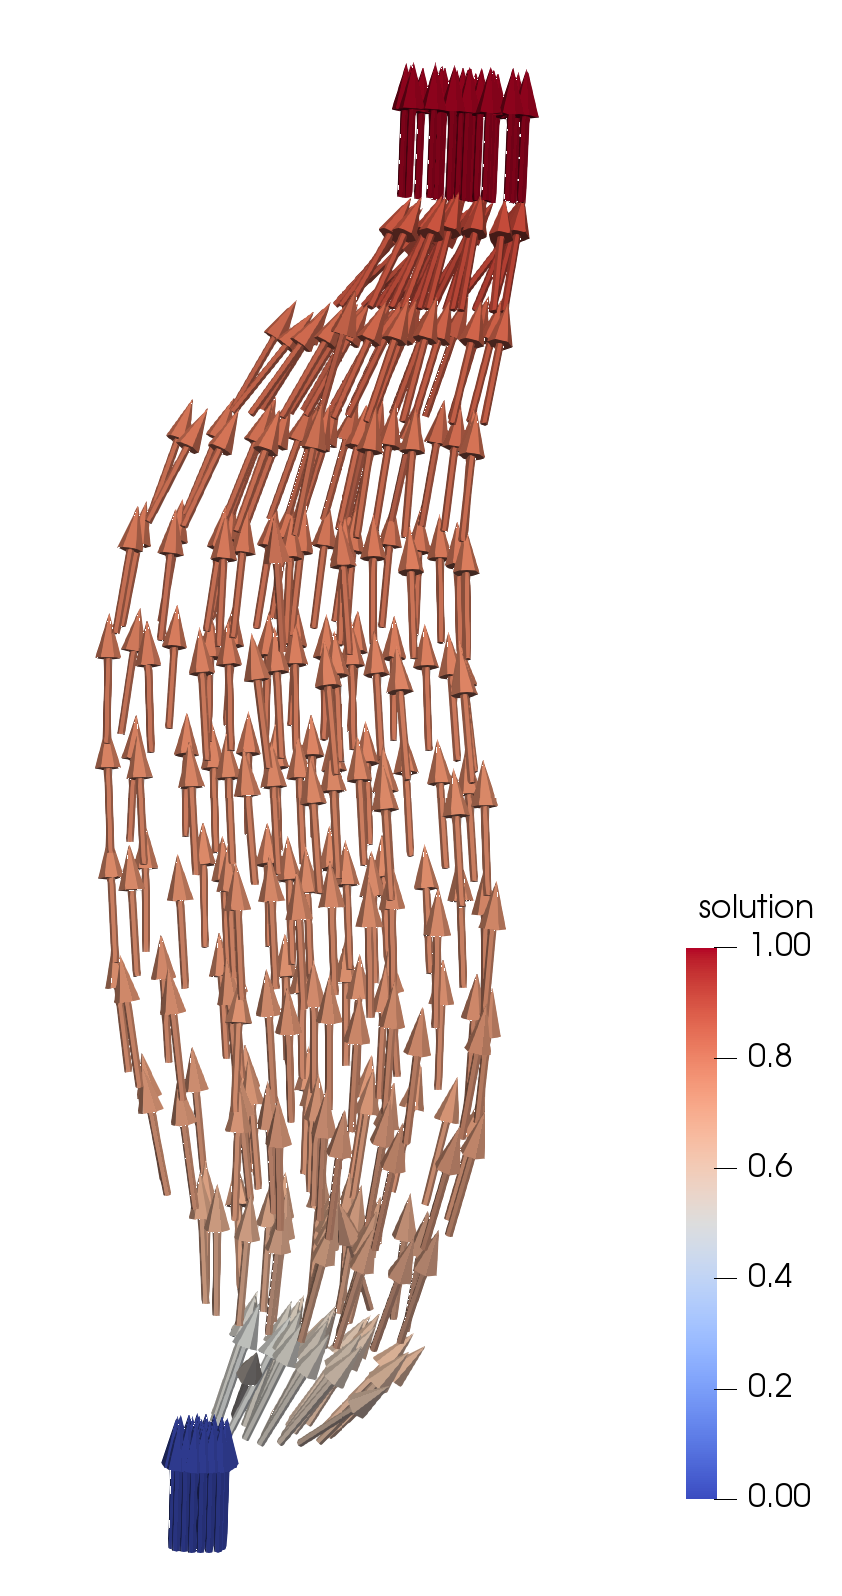
\includegraphics[height=10cm]{images/fiber_creation/potential_flow.png}%
    \caption{Solution (color coding) and direction vectors of the gradient field for the boundary value problem \cref{eq:fiberest_laplace} with Dirichlet boundary conditions \cref{eq:fiberest_dirichlet}.}%
    \label{fig:potential_flow}%
  \end{subfigure}
  \quad
  \begin{subfigure}[t]{0.48\textwidth}%
    \centering%
    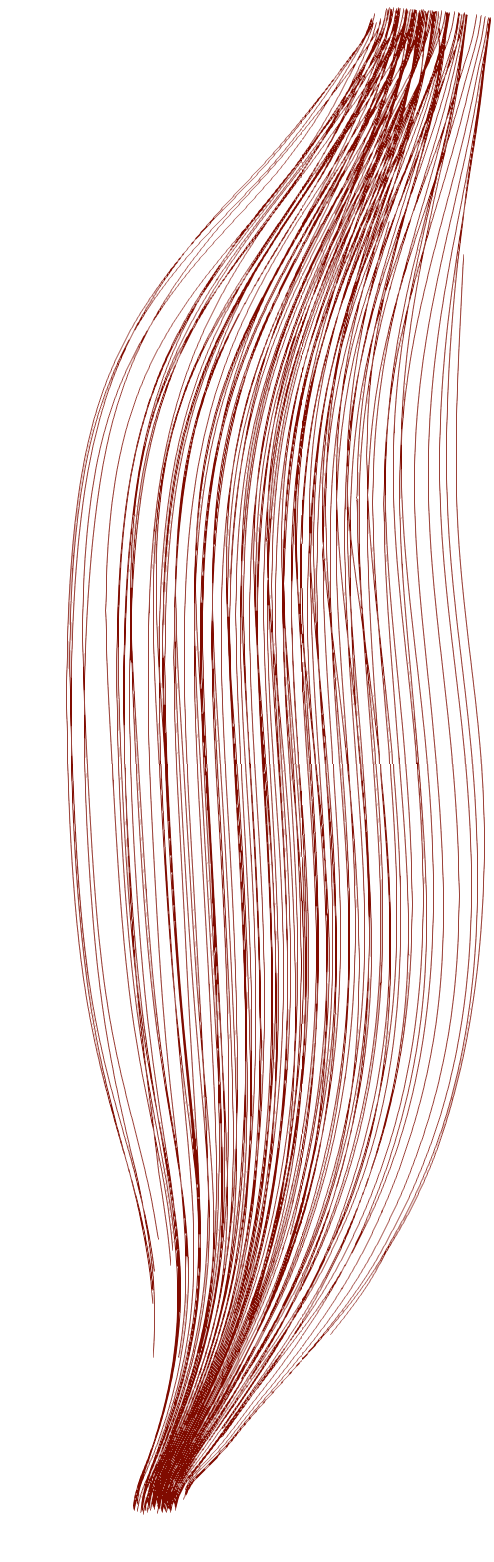
\includegraphics[height=10cm]{images/fiber_creation/streamlines_red.png}%
    \caption{Resulting streamlines that were traced through the gradient field.}%
    \label{fig:fiber_tracing_streamlines}%
  \end{subfigure}
  \caption{Setup and solution of the Laplace problem for the biceps geometry that is used to estimate muscle fibers by streamline tracing.}%
  \label{fig:potential_flow_streamlines}%
\end{figure}%

\subsection{Algorithm for Streamline Tracing}\label{sec:algorithm_for_streamline_tracing}
The algorithm for streamline tracing uses an efficient method to traverse the mesh, which makes use of its structuredness.
At first, the element $E^{(0)}$ in the mesh that contains the first seed point $\bfp^0$ needs to be found. By construction of the mesh generation algorithms, this is always the element with the lowest index. 
However, if the seed point is not found there, the scheme is robust enough to search in all other elements.

Starting from the seed point $\bfp^0 = \bfp^{(i)}$ in element $E^{(i)}$, the next point $\bfp^{(i+1)}$ of a streamline is computed as %
\begin{align*}
  \bfp^{(i+1)} = \bfp^{(i)} + h\,\nabla p (\bfp^{(i)}).
\end{align*}
After $\bfp^{(i+1)}$ has been computed, the mesh element $E^{(i+1)}$ where it is located needs to be identified. This is needed to evaluate the gradient value $\nabla p (\bfp^{(i+1)})$ at the new point by interpolation according to the FE representation of $p$.

At first, the element $E^{(i)}$ of $\bfp^{(i)}$ is checked whether it also contains $\bfp^{(i+1)}$. If not, the neighboring element in the direction of the streamline is considered. This neighboring element is chosen among all up to 26 possible neighbors such that the direction from the previous element $E^{(i-1)}$ to the current element $E^{(i)}$ continues.

If this element is also not the right one, all other neighbors of $E^{(i)}$ are subsequently checked, ordered by their plausibility according to the previous streamline direction. If none of the 27 considered elements contains the computed point, a search among all elements of the entire mesh is performed. This case happens only for unsuited choices of the integration width $h$, i.e., if the streamline tracing skips whole elements.

The end of a streamline is detected when the streamline reaches the final $z$ plane, either at the bottom or top of the muscle volume. To make the algorithm more robust, also the case is considered where the streamline leaves the muscle domain to the side shortly before reaching the end of the muscle. This can happen due to discretization errors for streamlines that start close to the boundary of the muscle. In such a case, the missing rest of the streamline is interpolated from up to four existing neighboring parallel streamlines.

After the end of the streamline is found, tracing of the next streamline starts at the next seed point $\bfp^0_\text{next}$. The element where $\bfp^0_\text{next}$ is located can also be easily determined in the structured mesh.

The presented scheme avoids repeatedly traversing all elements of the mesh by predicting the next elements according to streamline direction and organization of seed points. This is facilitated by the structured mesh, which has well-defined element neighbor relations.
At the same time, the scheme is robust enough to also efficiently handle streamlines in other use cases. It can also be reused, e.g., in muscle fiber tracing applications of more complex shaped muscles where the fibers change directions.

\subsection{Results and Discussion}\label{sec:mesh_generation_0_results_and_discussion}
The presented \cref{alg:serial_algorithm_1,alg:serial_algorithm_2} generate a 3D mesh and 1D muscle fibers from a triangulated surface. Three different triangulation strategies for the slices and four different reference quadrangulations can be chosen. In the following, the different choices are evaluated.

The different triangulation methods for the slices discussed in \cref{sec:triangulation_of_the_slices} are visualized in the three columns of \cref{fig:tri_triangulations}. 
The top rows show the triangulation of $S_M$ and the harmonic map $u$ as color coded values from violet to yellow. $u$ is the horizontal coordinate on the reference domain. A point with violet color in $S_M$ will be mapped to the left-most point in the parameter space $\Omega_P$. Similarly, a yellow point will be mapped to a point far at the right in $\Omega_P$.

The middle and bottom rows in \cref{fig:tri_triangulations} show the image of the triangulation in $\Omega_P$ under the harmonic map, for the unit square and the unit circle, respectively. The mapping between the colored boundary points stems from the Dirichlet boundary conditions in the formulation of the harmonic map. In consequence, the boundary points are by construction equally spaced both in the muscle domain $S_M$ and in the parameter domain $\Omega_P$.

It can be seen that the triangulation appears distorted in the parameter domain. The effect is most significant for the square in \cref{fig:triu_1} and \cref{fig:triu_2}. For the latter, the center point of the muscle domain $S_M$ gets mapped far off the center of the squared parameter domain. This effect does not occur for the circle.

The reason for this lies in the triangulation of $S_M$ together with the boundary shape. In the third method, only the value at the center point is a degree of freedom in the computation of $u$ while the values at the boundary points are fixed. By the triangulation, the value of $u$ varies linearly from the boundary towards the center point.
By comparing the colored boundary points in the muscle slice in the top row with the square in the second row, it can be seen that the prescribed values for $u$ are 0 at all blue points, 1 at all yellow points and linearly increasing from 0 to 1 at the green and red points, increasing from left to right.
The yellow points of $S_M$ with the prescribed constant value of $u=1$ are approximately located on a vertical line. The first two derivatives of $u$ in vertical coordinate direction are therefore almost zero, in consequence, the Laplace equation forces the derivatives in horizontal direction to also be approximately zero. Therefore, the solution value at the center point is close to $1$. This leads to the mapped center point being close to the right boundary in the square parameter domain. The same happens for the vertical coordinate $v$ of the harmonic map.

For the circle, neighboring boundary points are not located on horizontal or vertical lines and, thus, the Dirichlet bondary conditions for $u$ and $v$ vary along the boundary. Therefore, a better mapping is obtained. The shape of the muscular slice is more similar to the circle than to the square.

Another result that can be seen in \cref{fig:tri_triangulations} is the effect of the failure of the first method to handle concave slices on the harmonic map. As the top left image shows, the first triangulation method produces triangles outside the domain. The triangles are located around the red boundary points. In the square parameter domain, these triangles are degenerated and lie on the bottom boundary. In the circle parameter domain where the respective triangles can be seen at the bottom, they even intersect other triangles. This yields an invalid triangulation.

The reasons for degenerate triangles in the square parameter domains are not solely the concave muscle slices. Also, the straight sides of the unit square lead to degenerate triangles whenever three boundary points of the same side form a triangle.
In the example in \cref{fig:tri_triangulations}, this occurs for the square in column (\subref{fig:triu_0}). As can be seen in the triangulated slice in the top row, there are three triangles that are entirely made up of blue boundary points. These triangles get mapped onto the left side of the square parameter domain where they have a vanishing surface area.

The same effect also occurs with the second triangulation method in column (\subref{fig:triu_1}) of \cref{fig:tri_triangulations} where a triangle at the bottom right is comprised of three red boundary points and, therefore, gets mapped to the bottom side of the square. Because of the guaranteed minimum angle in the second triangulation method, this circumstance occurs less often and only for muscle cross-sections where the boundary makes sharp turns, such as the muscle slice in this example. The third triangulation method is guaranteed to avoid this problem as all triangles are connected with the center point.

% ------------------
% parameter space triangulations
\begin{figure}%
  \centering%
  \begin{subfigure}[t]{0.31\textwidth}%
    \centering%
    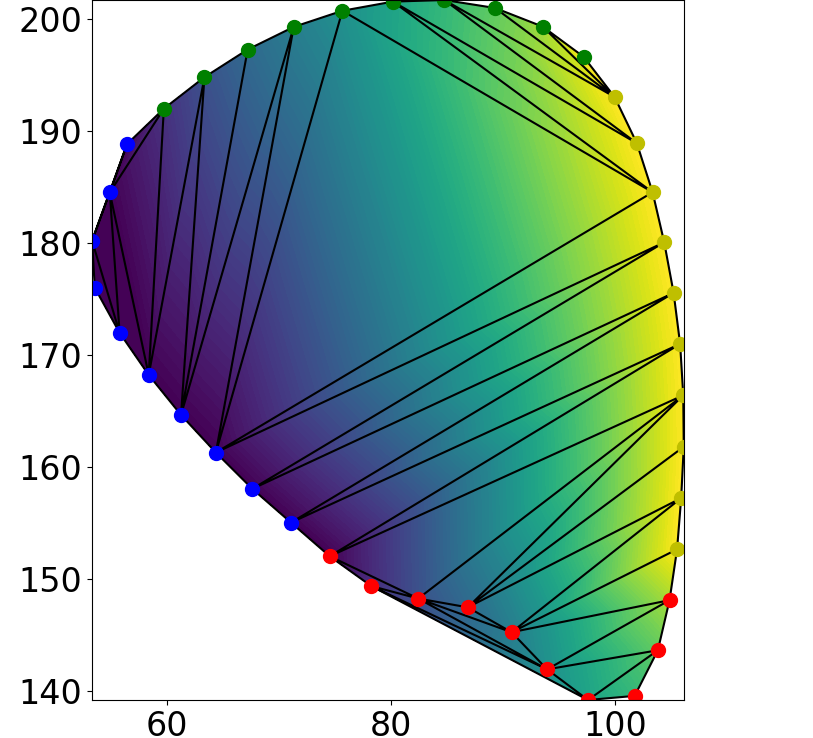
\includegraphics[width=\textwidth]{images/fiber_creation/u_0.png}%
    \caption{First method,\\Quickhull agorithm}%
    \label{fig:triu_0}%
  \end{subfigure}
  \quad
  \begin{subfigure}[t]{0.31\textwidth}%
    \centering%
    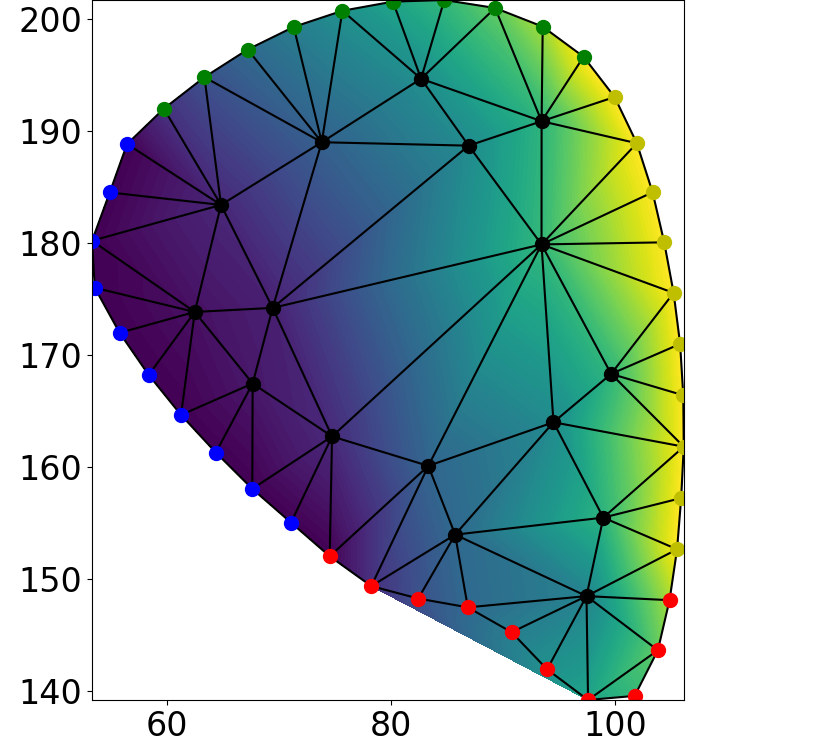
\includegraphics[width=\textwidth]{images/fiber_creation/u_1.png}%
    \caption{Second method,\\Delaunay refinement}%
    \label{fig:triu_1}%
  \end{subfigure}
  \quad
  \begin{subfigure}[t]{0.31\textwidth}%
    \centering%
    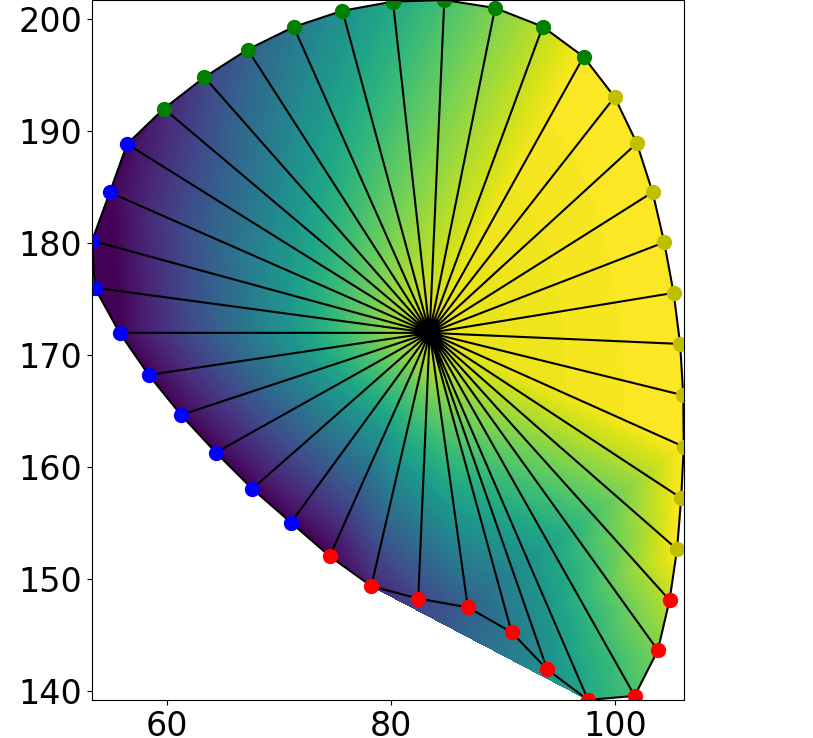
\includegraphics[width=\textwidth]{images/fiber_creation/u_2.png}%
    \caption{Third method,\\center of gravity}%
    \label{fig:triu_2}%
  \end{subfigure}\\
  
  % square
  \begin{subfigure}[t]{0.31\textwidth}%
    \centering%
    \includegraphics[width=0.9\textwidth, trim=37mm 14mm 6mm 6mm, clip]{images/fiber_creation/mesh_plots/out_0_1_0_tri.png}%
    %\caption{}%
    \label{fig:w_01}%
  \end{subfigure}
  \quad
  \begin{subfigure}[t]{0.31\textwidth}%
    \centering%
    \includegraphics[width=0.9\textwidth, trim=37mm 14mm 6mm 6mm, clip]{images/fiber_creation/mesh_plots/out_1_1_0_tri.png}%
    %\caption{}%
    \label{fig:w_11}%
  \end{subfigure}
  \quad
  \begin{subfigure}[t]{0.31\textwidth}%
    \centering%
    \includegraphics[width=0.9\textwidth, trim=37mm 14mm 6mm 6mm, clip]{images/fiber_creation/mesh_plots/out_2_1_0_tri.png}%
    %\caption{}%
    \label{fig:w_21}%
  \end{subfigure}\\
  
  % circle
  \hspace{-12mm}
  \begin{subfigure}[t]{0.31\textwidth}%
    \centering%
    \includegraphics[width=0.9\textwidth, trim=37mm 14mm 6mm 6mm, clip, angle=225,origin=c]{images/fiber_creation/mesh_plots/out_0_0_0_tri.png}% trim=left bottom right top, clip]
    %\caption{}%
    \label{fig:w_00}%
  \end{subfigure}
  \quad
  \begin{subfigure}[t]{0.31\textwidth}%
    \centering%
    \includegraphics[width=0.9\textwidth, trim=37mm 14mm 6mm 6mm, clip, angle=225,origin=c]{images/fiber_creation/mesh_plots/out_1_0_0_tri.png}%
    %\caption{}%
    \label{fig:w_10}%
  \end{subfigure}
  \quad
  \begin{subfigure}[t]{0.31\textwidth}%
    \centering%
    \includegraphics[width=0.9\textwidth, trim=37mm 14mm 6mm 6mm, clip, angle=225,origin=c]{images/fiber_creation/mesh_plots/out_2_0_0_tri.png}%
    %\caption{}%
    \label{fig:w_20}%
  \end{subfigure}
  
  \caption{Initial slice triangulation and harmonic maps in 3D mesh generation: Top row: Different triangulation methods for $S_M$, the color represents the solution $u$ of the harmonic map. Middle and bottom row: triangulation mapped to the parameter domain $\Omega_P$, for the unit square (middle) and the unit circle (bottom). Each column corresponds to one triangulation method.}%
  \label{fig:tri_triangulations}%
\end{figure}%

In conclusion, the second triangulation method with the unit circle and the third triangulation method with both unit square and unit circle show good behavior for use in our meshing algorithm. Next, their interplay with the quadrangulation of the parameter space needs to be investigated.

% bis hierher Änderungen eingearbeitet

In the next step, the algorithm creates a quadrilateral mesh in the parameter domain and computes its image in the muscle domain using the inverse of the harmonic map. The results are shown in \cref{fig:tri_meshes} for the three different initial triangulation methods (columns) and the four different schemes to create the quadrilateral mesh (rows).

In the images in column (\subref{fig:tu_2}) and rows (\subref{fig:tquad_1}) and (\subref{fig:tquad_2}), it can be seen that the previously observed effect of a bad mapping for squares and the third triangulation method also leads to a mesh in $S_M$ of poor quality.
The result for the two square schemes in column (\subref{fig:tu_1}) is better but still not satisfactory. Good results with the square reference domain are only observed for the first triangulation method in this example.

It can be seen that the approximation quality of the boundary of the domain varies. Most of all, the combination of the first triangulation method (column (\subref{fig:tu_0})) and the square parameter domain (rows (\subref{fig:tquad_1}) and (\subref{fig:tquad_2})) reproduces the shape of the slice poorly. 
The mismatch occurs at the blue and red boundary points. Additionally, the second triangulation method (column (\subref{fig:tu_1})) for the squares fails to correctly represent the round boundary at the bottom of the domain.
The degenerate triangles in the parameter domain are the cause for this effect. The harmonic map $\bfy: S_M \to \Omega_P$ is not injective and, therefore, its inverse does not exist. In our implementation, the points on the degenerate triangles in $\Omega_P$ are mapped to an arbitrarily selected location inside the corresponding triangles in $S_M$. Thus, the mapping is correctly inverted at locations of valid triangles and only creates different boundary points in the invalid areas.


Furthermore, it can be seen that an inaccurate representation of the boundary also occurs with the parameter mesh in the unit circle generated by scheme 1. In this case, the reason is the low number of elements at the boundary in the parameter domain quadrangulation.

The two schemes for the circle parameter domain in rows (\subref{fig:tquad_0}) and (\subref{fig:lquad_3}) both generate reasonable meshes for all triangulation methods, despite the different structure of the generated meshes. The best results for both schemes have been obtained with the third triangulation method.

% ------------------
% resulting meshes
\begin{figure}%
  \centering%
  \hspace{0.24\textwidth}
  \begin{subfigure}[t]{0.24\textwidth}%
    \centering%
    \includegraphics[width=\textwidth]{images/fiber_creation/u_0.png}%
    \caption{First method}%
    \label{fig:tu_0}%
  \end{subfigure}
  \begin{subfigure}[t]{0.24\textwidth}%
    \centering%
    \includegraphics[width=\textwidth]{images/fiber_creation/u_1.png}%
    \caption{Second method}%
    \label{fig:tu_1}%
  \end{subfigure}
  \begin{subfigure}[t]{0.24\textwidth}%
    \centering%
    \includegraphics[width=\textwidth]{images/fiber_creation/u_2.png}%
    \caption{Third method}%
    \label{fig:tu_2}%
  \end{subfigure}\\
  
  % square
  \begin{subfigure}[t]{0.24\textwidth}%
    \centering%
    \includegraphics[width=\textwidth]{images/fiber_creation/quad_1.png}%
    \caption{Square, scheme 1}%
    \label{fig:tquad_1}%
  \end{subfigure}
  \begin{subfigure}[t]{0.24\textwidth}%
    \centering%
    \includegraphics[width=\textwidth, trim=26mm 14mm 6mm 6mm, clip]{images/fiber_creation/mesh_plots/out_0_1_0_w.png}%
    %\caption{}%
    \label{fig:tri_01}%
  \end{subfigure}
  \begin{subfigure}[t]{0.24\textwidth}%
    \centering%
    \includegraphics[width=\textwidth, trim=30mm 14mm 6mm 6mm, clip]{images/fiber_creation/mesh_plots/out_1_1_0_w.png}%
    %\caption{}%
    \label{fig:tri_11}%
  \end{subfigure}
  \begin{subfigure}[t]{0.24\textwidth}%
    \centering%
    \includegraphics[width=\textwidth, trim=30mm 14mm 6mm 6mm, clip]{images/fiber_creation/mesh_plots/out_2_1_0_w.png}%
    %\caption{}%
    \label{fig:tri_21}%
  \end{subfigure}\\[-4mm]
  
  % square adjusted
  \begin{subfigure}[t]{0.24\textwidth}%
    \centering%
    \includegraphics[width=\textwidth]{images/fiber_creation/quad_2.png}%
    \caption{Square, scheme 2}%
    \label{fig:tquad_2}%
  \end{subfigure}
  \begin{subfigure}[t]{0.24\textwidth}%
    \centering%
    \includegraphics[width=\textwidth, trim=26mm 14mm 6mm 6mm, clip]{images/fiber_creation/mesh_plots/out_0_2_0_w.png}%
    %\caption{}%
    \label{fig:tri_02}%
  \end{subfigure}
  \begin{subfigure}[t]{0.24\textwidth}%
    \centering%
    \includegraphics[width=\textwidth, trim=30mm 14mm 6mm 6mm, clip]{images/fiber_creation/mesh_plots/out_1_2_0_w.png}%
    %\caption{}%
    \label{fig:tri_12}%
  \end{subfigure}
  \begin{subfigure}[t]{0.24\textwidth}%
    \centering%
    \includegraphics[width=\textwidth, trim=30mm 14mm 6mm 6mm, clip]{images/fiber_creation/mesh_plots/out_2_2_0_w.png}%
    %\caption{}%
    \label{fig:tri_22}%
  \end{subfigure}\\[-4mm]
  
  % circle
  \begin{subfigure}[t]{0.24\textwidth}%
    \centering%
    \includegraphics[width=\textwidth]{images/fiber_creation/quad_0.png}%
    \caption{Circle, scheme 1}%
    \label{fig:tquad_0}%
  \end{subfigure}
  \begin{subfigure}[t]{0.24\textwidth}%
    \centering%
    \includegraphics[width=\textwidth, trim=26mm 14mm 6mm 6mm, clip]{images/fiber_creation/mesh_plots/out_0_0_0_w.png}% trim=left bottom right top, clip]
    %\caption{}%
    \label{fig:tri_00}%
  \end{subfigure}
  \begin{subfigure}[t]{0.24\textwidth}%
    \centering%
    \includegraphics[width=\textwidth, trim=26mm 14mm 6mm 6mm, clip]{images/fiber_creation/mesh_plots/out_1_0_0_w.png}%
    %\caption{}%
    \label{fig:tri_10}%
  \end{subfigure}
  \begin{subfigure}[t]{0.24\textwidth}%
    \centering%
    \includegraphics[width=\textwidth, trim=30mm 14mm 6mm 6mm, clip]{images/fiber_creation/mesh_plots/out_2_0_0_w.png}%
    %\caption{}%
    \label{fig:tri_20}%
  \end{subfigure}\\[-4mm]
  
  % circle adjusted
  \begin{subfigure}[t]{0.24\textwidth}%
    \centering%
    \includegraphics[width=\textwidth]{images/fiber_creation/quad_3.png}%
    \caption{Circle, scheme 2}%
    \label{fig:lquad_3}%
  \end{subfigure}
  \begin{subfigure}[t]{0.24\textwidth}%
    \centering%
    \includegraphics[width=\textwidth, trim=30mm 14mm 6mm 6mm, clip]{images/fiber_creation/mesh_plots/out_0_3_0_w.png}%
    %\caption{}%
    \label{fig:tri_03}%
  \end{subfigure}
  \begin{subfigure}[t]{0.24\textwidth}%
    \centering%
    \includegraphics[width=\textwidth, trim=30mm 14mm 6mm 6mm, clip]{images/fiber_creation/mesh_plots/out_1_3_0_w.png}%
    %\caption{}%
    \label{fig:tri_13}%
  \end{subfigure}
  \begin{subfigure}[t]{0.24\textwidth}%
    \centering%
    \includegraphics[width=\textwidth, trim=30mm 14mm 6mm 6mm, clip]{images/fiber_creation/mesh_plots/out_2_3_0_w.png}%
    %\caption{}%
    \label{fig:tri_23}%
  \end{subfigure}
  \caption{Initial triangulations, harmonic maps and final quadrangulations of muscle slices for 3D mesh generation: Meshes in the muscle slice $S_M$ for quadrangulations (rows) and triangulations (columns).}%
  \label{fig:tri_meshes}%
\end{figure}%

% quantitative quality plots of results

%The mesh quality could easily be improved by a smoothing step, e.g., by applying Laplacian smoothing \cite{field1988laplacianSmoothingAndDelaunayTriangulations}. This technique iteratively improves the local mesh quality. Because of the local scheme, the quality of the final result depends on the quality of the initial mesh. 
%Therefore, the following study forgoes additional smoothing steps and evaluates the direct outcome of the meshing algorithm.

Next, a quantitative comparison of the resulting mesh quality for different parameters of the presented algorithm is carried out. 
The algorithm was executed for all variants with 43 slices of the biceps muscle, resulting in 43 meshes for every combination of triangulation method and quadrangulation scheme. To asses the quality of the generated meshes, the edge lengths of the elements were collected and normalized to have a mean of 1 in each mesh. 
The normalization was done to allow for a comparison between meshes with different bounding box sizes.
The standard deviation of the normalized lengths was determined in each mesh. The total mean of all standard deviations was computed. This value is a measure for the quality of the mesh. A low value means that, in every slice, the generated mesh has similar edge lengths and, in consequence, the overall mesh has good quality.

\begin{figure}%
  \centering%
  \includegraphics[width=\textwidth]{images/fiber_creation/mesh_quality.pdf}%
  \caption{3D mesh generation quality assessment: Mesh quality (red, lower is better) and generation runtime (yellow) for the three different triangulation methods and the different parameter space quadrangulation schemes. $\square 1$ and $\square 2$ designate the two quadrangulation schemes on the unit square parameter domain, $\ocircle 1$ and $\ocircle 2$ are the schemes on the unit circle parameter domain, as introduced in \cref{fig:quads}. A low value for the standard deviation of relative element lengths indicates good quality.}%
  \label{fig:mesh_quality}%
\end{figure}

\Cref{fig:mesh_quality} visualizes the results. Three groups of bars are displayed for the three triangulation methods. For every type of mesh in the parameter space, i.e., unit square ($\square$) or unit circle ($\ocircle$) and scheme 1 or 2, the standard deviation is given by the red bar and the generation runtime of the overall algorithm is given by the yellow bar. The corresponding axis labels for standard deviation and duration are given on the left and right of the diagram.

The diagram shows the lowest standard deviation of edges and therefore the best mesh quality for the first triangulation method and the square ($\square 1$ and $\square 2$), with scheme 1 having a slightly better value than scheme 2. This shows that the modified placement of the nodes in scheme 2 has no positive effect compared to scheme 1.
However, from the observations in \cref{fig:tri_triangulations}, it is known that the boundaries are not represented correctly.
This behavior does not influence the result because of the chosen metric of uniform relative edge lengths.
Similarly good results can be seen for scheme 2 in the circular parameter domain and the second and third triangulations.

Moreover, it can be seen that certain connections between parameter domain and suited triangulation scheme exist. The square parameter domain works best with the first triangulation method. The second scheme for the parameter mesh on the unit circle works best with the triangulation methods 2 and 3.

The first scheme for the parameter mesh on the unit circle ($\ocircle 1$) shows bad results for all triangulation methods. This can be explained by looking at the generated meshes in row (\subref{fig:tquad_0}) of \cref{fig:tri_meshes}. By construction, the elements have a bad aspect ratio. This results in the high standard deviation values. However, the generated meshes still look uniform to a certain extent and can be useful in applications where such type of mesh is needed. The score could be improved by adding more nodes in circumferential direction.

The runtime of the algorithm is approximately the same for the different parameter domain meshes. It mainly depends on the triangulation of the slices. The first triangulation using the \emph{SciPy} package takes the most time, followed by the Delaunay refinement. The fastest triangulation is the custom one where only one additional point needs to be placed. In conclusion, when runtime is an issue, the third triangulation should be chosen. It achieves good quality meshes only with the second scheme of the circular parameter domain. This combination also does not suffer from the bad approximation quality of the boundary, as is the case for the unit circle with the first triangulation method.

\Cref{fig:tendon_meshes} shows three structured meshes $\Omega_{T,i}$ for the tendons of the biceps brachii muscle that were created using \cref{alg:serial_algorithm_1}. The tendon at the bottom of the muscle is represented by a single mesh. At the top, there are two tendons that extend the two muscle heads of the biceps. Because the meshes need to be structured, two tendon meshes are created at the top. It can be seen that the algorithm creates meshes with similar sized elements despite the difficult, wound geometry of the surfaces.

\begin{figure}
  \centering
  \begin{tabular}{cc}
    \begin{tabular}[b]{c}
      \begin{subfigure}[b]{0.60\textwidth}%
        \centering%
        \includegraphics[width=\textwidth]{images/fiber_creation/tendon2_.png}
        \caption{Two meshes for the top tendons with $9 \times 9 \times 21 = \num{1701}$ nodes each.}%
        \label{fig:tendon2}%
      \end{subfigure} \\
      \begin{subfigure}[b]{0.60\textwidth}%
        \centering%
        \includegraphics[width=\textwidth]{images/fiber_creation/tendon1.png}
        \caption{One mesh for the bottom tendon with $5 \times 5 \times 25 = \num{525}$ nodes.}%
        \label{fig:tendon1}%
      \end{subfigure}
    \end{tabular}
    &
    \begin{subfigure}[b]{0.30\textwidth}%
      \centering%
      \includegraphics[width=\textwidth]{images/fiber_creation/muscle_with_tendons.png}
      \caption{The tendon meshes in the volume of the whole biceps muscle.}%
      \label{fig:muscle_with_tendons}%
    \end{subfigure}
  \end{tabular}
  \caption{3D mesh generation results: Tendon meshes that were created using the serial algorithm for mesh creation.}%
  \label{fig:tendon_meshes}%
\end{figure}%

\begin{reproduce_no_break}
  The described algorithms are part of the \code{fiber_tracing} examples. Execute the following commands to get the results in this chapter:
  \begin{lstlisting}[columns=fullflexible,breaklines=true,postbreak=\mbox{\textcolor{gray}{$\hookrightarrow$}\space}]
    cd $\$$OPENDIHU_HOME/examples/fiber_tracing/streamline_tracer/scripts
    . run_evaluation.sh
  \end{lstlisting}
  Then, the visualizations will be created under \code{../processed_meshes}. Create \cref{fig:mesh_quality} with \code{plot_mesh_quality.py}.
  How to create the tendon meshes is explained at the end of \cref{sec:repro_tendon_meshes}.
\end{reproduce_no_break}



\setcounter{section}{4}
\section{Parallel Algorithm to Create Muscle and Fiber Meshes}\label{sec:parallel_algorithm}
%

The previously presented algorithm to create 3D and 1D meshes is not parallelized. 
%This restricts the resources that can be employed during the execution of the algorithm to those accessible by one hardware core.
Thus, the size of the handled meshes is limited by the available memory of the computer.
An algorithm that can be used with distributed memory parallelization could, in contrast, benefit from more total memory that is accessible at different compute nodes. Furthermore, the tracing of the streamlines could be performed in parallel which has the potential to reduce runtimes.

In the following, we present an extended algorithm based on the one presented in \cref{sec:ser_alg_meshes} that can be run in parallel on multiple cores. The extended algorithm employs a partitioning of the 3D volume. Every process only stores data corresponding to its own partition. This allows to run the algorithm on a distributed memory system, where data transfer between the processes occurs by sending messages using the Message Passing Interface (MPI). It is possible to create meshes with larger sizes than could fit into a single nodes' memory. This enables us to run the algorithm for meshes with very high resolution that can be used for simulations in the field of High Performance Computing. 
These meshes are partitioned into subdomains for every compute core and can be read from and written to disk concurrently.

\subsection{Overview of the Parallel Algorithm to Create Muscle and Fiber Meshes}

The steps of the algorithm and its input and output are given in \cref{alg:parallel_algorithm_1}. Input and output are the same as for the \cref{alg:serial_algorithm_1} presented in \cref{sec:ser_alg_meshes}. The input is a triangulated tubular surface of the muscle that can be obtained as described in \cref{sec:preprocessing_of_the_muscle_geometry}. A second input, the variable called \emph{boundary\_points}, is used only during recursive calls and is not set at the beginning. The output consists of the 3D mesh of the muscle volume $\Omega_M$ and embedded 1D fiber meshes $\Omega_{F,i}$. 

During execution of the algorithm, the 3D mesh of the muscle is recreated iteratively with increasing resolution and increasing number of subdomains. The algorithm is formulated recursively. 
At the finest resolution when the recursion terminates, the fiber meshes are finally generated together in all subdomains.

At first, a single process executes all the steps of \cref{alg:parallel_algorithm_1} from lines \ref{line:3.2} to \ref{line:3.11a}. This corresponds to recursion level $\ell=0$. Then, in line \ref{line:3.12}, the procedure is called again and in the first recursion executed by eight processes with eight subdomains. On the $\ell$th recursion level, the number of involved processes and subdomains is $8^\ell$. After a specified maximum recursion depth $\ell_\text{max}$ is reached, all involved processes execute the first branch of the \code{if} statement in line \ref{line:3.8} and generate the final 3D and 1D output meshes in line \ref{line:3.9}.

The steps in \cref{alg:parallel_algorithm_1} are executed concurrently by the involved processes at the respective levels.
Some of the steps only operate on the locally stored data and, thus, are independent of other processes. Other steps involve communication between processes. Whether an instruction effects only the own domain of the process or involves global communication is denoted in parantheses at the beginning of the lines in \cref{alg:parallel_algorithm_1}.

\begin{algorithm}
  \begin{algorithmic}[1]%
    \Procedure{Create\_3D\_meshes\_parallel}{}
    \Require Triangulated tubular surface
    \Require boundary\_points: $4\times 4$ points per slice
    \Ensure Structured 3D volume mesh
    \Ensure 1D fiber meshes
    \Statex
    \State (own domain) Create\_3D\_mesh(boundary\_points)        \label{line:3.2}
    \State (own domain) Fix and smooth 2D meshes  \label{line:3.3}   
    \State (global)$\hskip2.4em$     Solve Laplace problem       \label{line:3.4}
    \State (global)$\hskip2.4em$      Communicate ghost elements to neighboring subdomains      \label{line:3.5}
    \State (own domain) Trace streamlines for new subdomain boundaries      \label{line:3.6}
    \State (global)$\hskip2.4em$      new\_boundary\_points $\leftarrow$ Construct new subdomains      \label{line:3.7}
    \Statex
    \If{recursion ends}         \label{line:3.8}
    \State (own domain) Trace streamlines for fiber meshes      \label{line:3.9}
    \Else      \label{line:3.10}
    \State (global)$\hskip2.4em$      communicate boundary points      \label{line:3.11a}
    \State (global)$\hskip2.4em$      Create\_3D\_meshes\_parallel(new\_boundary\_points)      \label{line:3.11}
    \EndIf      \label{line:3.12}
    \EndProcedure
  \end{algorithmic}%
  \caption{Parallel algorithm to create muscle and fiber meshes}%
  \label{alg:parallel_algorithm_1}%
\end{algorithm}%

\subsection{Overview of the Subdomain Refinement}

The goal during the recursive calls is to determine smooth boundaries for the new subdomains. Each process splits its own subdomain into eight subdomains and then proceeds to the next recursion level.
The subdomain boundaries are determined by tracing streamlines in a divergence-free vector field through the entire muscle volume, similar to the approach in \cref{alg:serial_algorithm_2}. The divergence-free vector field is computed from the solution of a Laplace problem, which is solved in parallel on the entire mesh of the muscle in every recursion. The mesh width of this mesh gets halved in every recursion, subsequently leading to an increasingly fine mesh.

The subdomain boundaries are always aligned to streamlines in the mesh that was created last.
On each recursion level, the existing subdomain boundaries and the new boundaries for the subdomains on the next recursion level are all created anew and, thus, change slightly as the mesh refines.

As the subdomain boundaries in the interior of the volume refine, so do the outer boundaries given by the surface of the muscle. The given triangulation of the surface is sampled again on each recursion level yielding increasingly fine representations.

At the final recursion level $l_\text{max}$, the muscle is partioned into $8^{l_\text{max}}$ subdomains and a respective fine 3D mesh in the muscle volume exists. Then, the algorithm traces the specified amount of streamlines through the whole mesh to produce 1D meshes for the muscle fibers. By construction of the subdomains, the streamlines enter and leave the subdomains through their top and bottom bounding planes. This allows parallel execution of the final streamline tracing step.

The reason that the algorithm constructs the partitioning iteratively and not once at the beginning using an initial mesh lies in the requirements for parallel streamline tracing. Each subdomain should be able to trace streamlines in longitudinal ($z$) direction of the muscle without communication to their neighbors in $x$ and $y$ directions. To ensure this property, the partitioning involves a small overlap of neighboring subdomains, i.e., a ghost layer. This ghost layer can consist of a lower number of elements if the mesh is iteratively refined than if the partitioning was created directly on a coarser mesh.

% --
\subsection{Data Structure of Boundary Points}\label{sec:data_structure_of_boundary_points}

In the following, \cref{alg:parallel_algorithm_1} is illustrated in more detail.
The execution starts with one process and the only input is the tubular muscle surface. It is given either as triangulation or in parametric form as NURBS surface.
The first step is to construct a quadrilateral mesh of this surface. This is done using the procedure explained in \cref{sec:slicing_of_the_geometry}, which creates horizontal slices of the muscle and places equidistant points on the \say{rings} of the boundaries of these slices. As explained earlier, the points are arranged such that the resulting quadrangulation of the surface has good quality. A result for the biceps muscle is visualized in \cref{fig:serial_alg_0}.

Initially, the parallel algorithm stores the points on these rings in the variable \code{boundary\_}\\\code{points}. If the procedure in \cref{alg:parallel_algorithm_1} is called recursively, the contents of this variable is passed as an argument from the previous recursion.
The set of points in \code{boundary\_points} defines the boundaries of the subdomain of the process where it is stored.

The points on each ring in the $x$-$y$-plane are organized such that they enclose a grid of $n_\text{el,x} \times n_\text{el,x}$ elements, where the number $n_\text{el,x}$ of elements per coordinate direction can be specified as parameter. In the following, an example with $n_\text{el,x}=4$ is considered. The grid is shown in \cref{fig:boundary_grid_1}, the $4\,n_\text{el,x}$ boundary points on the ring are visualized by red color. Note that \cref{fig:boundary_grid_1} depicts the ring as a square whereas in reality it has the potentially more irregular shape of the subdomain.

A number $(n_\text{el,z}+1)$ of these rings are stacked in $z$ direction to approximate the enclosing surface of the subdomain, where the number $n_\text{el,z}$ of elements in $z$ direction is again given by a parameter. Thus, the variable \code{boundary\_points} contains a total of $4\,n_\text{el,x}\,(n_\text{el,z}+1)$ points. Typical parameter values are $n_\text{el,x}=4$ and $n_\text{el,z}=50$. 

\begin{figure}%
  \centering%
  \begin{subfigure}[t]{0.48\textwidth}%
    \centering%
    \includegraphics[width=3cm]{images/parallel_fiber_estimation/boundary_grid.pdf}%
   \caption{Grid of $4 \times 4$ boundary points, which occurs at the beginning of the procedure of \cref{alg:parallel_algorithm_1}.}%
    \label{fig:boundary_grid_1}%
  \end{subfigure}
  \quad
  \begin{subfigure}[t]{0.48\textwidth}%
    \centering%
    \includegraphics[width=3cm]{images/parallel_fiber_estimation/boundary_grid_2.pdf}%
    \caption{Grid with $4 \times 8$ boundary points, which occurs after a refinement step at beginning of the procedure of \cref{alg:parallel_algorithm_1}.}%
    \label{fig:boundary_grid_2}%
  \end{subfigure}   
  \caption{Logical subdomain boundaries (red) and interior grid (gray) before and after the refinement at the beginning of \cref{alg:parallel_algorithm_1}.}%
  \label{fig:boundary_grid}%
\end{figure}%

% refine border points
As the goal on every recursion level is to construct a mesh with half the mesh width of the mesh on the previous level, the given boundary points are refined to twice the amount by inserting new points at the centers between neighboring points. The refinement happends in all three coordinate directions. For the example with $n_\text{el,x}=4$, the resulting grid with the $4\times 8$ refined boundary points is shown in \cref{fig:boundary_grid_2}. In $z$ direction, we get $(2\,n_\text{el,z}+1)$ slices with points.

% logical structure of new subdomains
The task in the recursive procedure is now to determine boundaries for eight subdomains. This is achieved by subdividing the given 2D slices into four 2D subdomains each. Additionally, the 3D volume is split at its vertical center. Thus, the upper and lower parts contain four subdomains each. 
\Cref{fig:subdomain} visualizes this scheme for the eight subdomains on recursion level $l=1$. The boundary points of the first and the eighth subdomain are shown. The boundary points have already been refined such that every slice in \cref{fig:subdomain} consists of $4 \times 8$ points and corresponds to the grid in \cref{fig:boundary_grid_2}
\begin{figure}%
  \centering%
  \includegraphics[height=8cm]{images/parallel_fiber_estimation/subdomains_2.png}%
  \caption{Parallel 3D mesh generation: Partitioning of the muscle volume into eight subdomains during the first call to the procedure in \cref{alg:parallel_algorithm_1}. The first (red) and the eighth subdomain (green) are shown.}%
  \label{fig:subdomain}%
\end{figure}%

%   ^v^v^

%For this reason, the given $4 \times 4$ boundary points are refined to twice the amount of boundary points by inserting new points at the centers between neighboring points. The resulting grid is shown in \cref{fig:boundary_grid_2}. Now, it would be possible to subdivide the grid to obtain four instances of the needed grid in \cref{fig:boundary_grid_1}.
%However, this would result in constant straight connection lines between the initial boundary points. In all further recursive calls, the additional points would all be placed on these lines and thereby not properly refine the subdomain boundaries. Instead, a different approach is desired where the subdomain's boundaries in the volume follow the directions of streamlines and fibers. Thus, the approach is to define the subdomain boundaries in the interior of the global domain by traced streamlines and sample the outer boundaries from the surface triangulation with the desired mesh width. The required steps of this approach are discussed next.

% --

\subsection{Generation and Smoothing of the 3D Mesh}
% create 3D mesh

After the \code{boundary\_points} variables has been set, the next step of \cref{alg:parallel_algorithm_1} is to construct a 3D mesh in the domain.
In line \ref{line:3.2} of \cref{alg:parallel_algorithm_1}, the harmonic map  algorithm \cref{alg:serial_algorithm_1} described in \cref{sec:ser_alg_meshes} is called. Its input consists of the boundary points that define the 2D slices of the volume. This means that \cref{alg:serial_algorithm_1} does not need to construct the slice boundary rings from the surface triangulation, instead, the formulation of \cref{alg:serial_algorithm_1} can directly start with line \ref{alg:1.2} to triangulate the slices and then compute the harmonic map. For the harmonic map computation, the second triangulation method is used with a circular reference domain quandrangulated by the second scheme. The result is a set of quadrangulated 2D slices that forms a 3D mesh by vertically connecting the elements of neighbor slices.

% smoothing
Next, line \ref{line:3.3} of \cref{alg:parallel_algorithm_1} improves the mesh quality of the 2D muscle slices $S_M$ from which the 3D mesh is formed. This action consists of two steps. The first step is to ensure that no self-intersecting or degenerate quadrilaterals exist in the slice. The second step applies Laplacian smoothing to improve the mesh quality of the slice.

Theoretically, the first step should not be necessary, as the chosen quadrangulation algorithm always produces valid elements. However, in practice, small or irregularly shaped, concave domains occur and together with rounding and numerical errors in the Laplace problem computations occasionally lead to invalid meshes with self intersecting elements, especially for higher recursion depths in \cref{alg:parallel_algorithm_1}. Executing the first step therefore increases the robustness of the implementation.

\begin{figure}%
  \centering%
  \def\svgwidth{0.7\textwidth}%
  \input{images/parallel_fiber_estimation/quads.pdf_tex}%
  \caption{Decomposition of quadrilateral elements into triangles as substep of the validity check of muscle slice quadrangulations. A quadrilateral element (left) and the four triangles (right) that can be constructed from its four points. These triangles are needed for the check in \cref{alg:parallel_algorithm_1} whether the quadrilateral element is valid.}%
  \label{fig:quads_tris}%
\end{figure}%

\begin{figure}%
  \centering%
  \begin{subfigure}[t]{0.48\textwidth}%
    \centering%
    \includegraphics[width=3cm]{images/parallel_fiber_estimation/triangle_score_3.pdf}%
    \caption{Convex quadrilateral with score $s=4$ and the contained triangles, which are all oriented counterclockwise.}%
    \label{fig:triangle_score_3}%
  \end{subfigure}
  \quad
  \begin{subfigure}[t]{0.48\textwidth}%
    \centering%
    \includegraphics[width=3cm]{images/parallel_fiber_estimation/triangle_score_4.pdf}%
    \caption{Concave quadrilateral with score $s=3$ and the contained triangles. Only the red triangle is oriented clockwise.}%
    \label{fig:triangle_score_4}%
  \end{subfigure}   
  \caption{Check for valid elements in the muscle slice quadrangulations that occurs in \cref{alg:parallel_algorithm_1}: Illustration of the score of valid concave and convex quadrilaterals.}%
  \label{fig:triangle_score}%
\end{figure}%

The algorithm performs this step by repeatedly iterating over all interior mesh points in every slice $S_M$ and fixing invalid elements. To find invalid elements, for every quadrilateral the four triangles that can be formed from the points of the quadrilateral are considered, as shown in \cref{fig:quads_tris}.
For every triangle with points $\bfp^0,\bfp^1$ and $\bfp^2$, the orientation of the triangle is determined. The orientation is counterclockwise if the oriented triangle area $A_{012}$ is positive. The oriented triangle area is the determinant of the $3 \times 3$ matrix that contains the row vectors $(p^i_x,p^i_y,1)$ for the triangle points $\bfp^i=(p^i_x,p^i_y)^\top$ and can be computed by the following formula \cite{sedgewick2011algorithms}:
%
\begin{align*}
  A_{012} = (p^1_x-p^0_x)\,(p^2_y-p^0_y) - (p^2_x-p^0_x)\,(p^1_y-p^0_y).
\end{align*}
If the orientation is counterclockwise, a score value of the triangle is set to one, if it is clockwise, the score is set to zero. The score values of the four triangles are added up to yield a score $s$ for the quadrilateral. Only if this score is $s \geq 3$, the quadrilateral is valid. \Cref{fig:triangle_score} illustrates the cases of valid quadrilateral elements. In a valid, convex element, all four triangles lie inside the element and, thus, the score is $s=4$. If only one triangle is located outside, the quadrilateral is also valid and concave. In this case the score has the value $s=3$.

At the current mesh point in the loop over all points that are not at the boundary of the mesh, the four adjacent quadrilaterals are considered. If any of them is invalid, the algorithm tries to improve the situation by deflecting the point by a random, small vector. A maximum of 200 random deflections from the original position with exponentially increasing deflection vector sizes are tried. After each modification of the point, the scores of the four adjacent quadrilateral elements are evaluated. If the sum of the four element scores increases, the point is kept and the iteration over all interior mesh points starts anew. 

Note that this does not necessarily mean that the invalid element was fixed, only its score was improved. If it was not fixed, it will be considered again in the next iteration. For example, a convex element that initially is oriented clockwise instead of counterclockwise has a score of $s=0$. In the first iteration, one point is deflected such that the quadrilateral intersects itself but has a higher score $s\geq 0$. At least one more iteration is needed until the quadrilateral is oriented correctly.
When all elements in the slice $S_M$ are valid, this step is complete.

\subsection{Laplacian Smoothing}
The second step is the smoothing step that improves the mesh quality of the 2D slices. \num{20} iterations of Laplacian smoothing \cite{field1988laplacianSmoothingAndDelaunayTriangulations} are executed. Laplacian smoothing in our case subsequently visits all interior points of the mesh and sets the location of a point to the center of gravity of its four direct neighbors.
%The order in which the points of the mesh are traversed is changed after every iteration: In the first iteration, the points are traversed starting at the bottom left. In the second iteration, the traversal starts at the top right and moves in opposite direction compared to the first iteration. The third and fourth iterations begin at the bottom right and top left nodes of the mesh. After these four iterations the scheme is repeated. The reason for this change of the traversal is to 
\Cref{fig:laplace_smoothing} shows the effect of Laplacian smoothing for a slice in a subdomain on the first recursion level. It can be seen how the smoothing equalizes the element side lengths and angles.

However, this smoothing step can invalidate a mesh by introducing overlapping quadrilaterals. An example for this case is given in \cref{fig:laplace_smoothing_0}. The initial mesh in \cref{fig:world_mesh_0} is concave and occurs during recursion level $l=2$. \Cref{fig:world_mesh_improved_0} shows the result of the smoothing, which contains one invalid element. The smoothing operation placed the fourth point of the element that also contains the three boundary points at the concavity outside of the mesh. As a remedy, the smoothing method checks the validity of the adjacent elements before a point is moved. If the move would result in an invalid element, the action is not carried out and the traversal continues with the next point instead.
\Cref{fig:world_mesh_improved_1} shows the resulting mesh if this check is enabled. The mesh has slightly different boundaries because the check influenced the behavior already on lower recursion levels.

% smoothing fix

\begin{figure}%
  \centering%
  \begin{subfigure}[t]{0.48\textwidth}%
    \centering%
    \includegraphics[height=7cm]{images/parallel_fiber_estimation/world_mesh.png}
    \caption{Initial 2D mesh of a subdomain at the boundary of the biceps muscle.}%
    \label{fig:world_mesh}%
  \end{subfigure}
  \quad
  \begin{subfigure}[t]{0.48\textwidth}%
    \centering%
    \includegraphics[height=7cm]{images/parallel_fiber_estimation/world_mesh_improved.png}
    \caption{The mesh of (\subref{fig:world_mesh}) after 20 iterations of Laplacian smoothing.}%
    \label{fig:world_mesh_improved}%
  \end{subfigure}    
  \caption{Quality improvement of 2D muscle slice quadrangulation: Effect of Laplacian smoothing of a 2D grid which occurs in line \ref{line:3.3} of \cref{alg:parallel_algorithm_1}.}%
  \label{fig:laplace_smoothing}%
\end{figure}%

\begin{figure}%
  \centering%
  \begin{subfigure}[t]{0.30\textwidth}%
    \centering%
    \includegraphics[width=\textwidth]{images/parallel_fiber_estimation/loop_025_p3728344_world_mesh.png}
    \caption{Initial 2D mesh.}%
    \label{fig:world_mesh_0}%
  \end{subfigure}
  \quad
  \begin{subfigure}[t]{0.30\textwidth}%
    \centering%
    \includegraphics[width=\textwidth]{images/parallel_fiber_estimation/loop_025_p3728344_world_mesh_improved_3.png}
    \caption{The mesh of (\subref{fig:world_mesh_0}) after 20 iterations of Laplacian smoothing, yielding an invalid quadrangulation.}%
    \label{fig:world_mesh_improved_0}%
  \end{subfigure}    
  \quad
  \begin{subfigure}[t]{0.30\textwidth}%
    \centering%
    \includegraphics[width=\textwidth]{images/parallel_fiber_estimation/loop_025_p30402_world_mesh_improved.png}
    \caption{The mesh of (\subref{fig:world_mesh_0}) after 20 iterations of Laplacian smoothing with the validity check, yielding a valid quadrangulation.}%
    \label{fig:world_mesh_improved_1}%
  \end{subfigure}    
  \caption{Quality improvement of 2D muscle slice quadrangulation: Effects of Laplacian smoothing on concave domains.}%
  \label{fig:laplace_smoothing_0}%
\end{figure}%

\subsection{Solution of the Laplace Problem}\label{sec:solution_of_the_laplace_problem}

After the 3D mesh has been created and smoothened, the next steps are to solve the Laplace problem in the muscle domain, to trace streamlines in the gradient of the solution vector field and finally to construct the eight subdomains for the recursive calls by subdividing the own domain along the streamlines.

% refine 3D mesh
Prior to the solution of the Laplace problem, the 3D mesh gets refined further by increasing the number of elements per coordinate direction by a specified factor $r\in \N$. The rationale is to increase the number of degrees of freedom and, thus, the resolution to get a smaller numerical error in the subsequent Laplace computation.
This refinement is in addition to the refinement of the initial boundary points by a factor of two described in \cref{sec:data_structure_of_boundary_points}. The mesh with $2\,n_\text{el,x} \times 2\,n_\text{el,x} \times 2\,n_\text{el,z}$ elements gets refined to $2\,r\,n_\text{el,x} \times 2\,r\,n_\text{el,x} \times 2\,r\,n_\text{el,z}$ elements. The new points are found by interpolating in the existing mesh.

For example, the 3D mesh of \cref{fig:boundary_grid} with $2\cdot 4 \times 2\cdot 4 \times 2\cdot 50$ elements gets refined with the factor $r=2$ to $16 \times 16 \times 200$ elements.
\Cref{fig:02_boundary_points} shows the refined boundary points in this example in a view in negative $z$ direction towards the bottom of the muscle. The red points are the boundary points of the $4 \times 8$ grid, the additional white points are added in between by the refinement with $r=2$. 
Because this refinement is carried out by interpolating between the initial points, the new points are located on straight lines between the initial points.
This can especially be seen at the lower left of the figure (indicated by arrows and lines) where always five neighboring points lie on a straight line. 

\begin{figure}%
  \centering%
  \begin{subfigure}[t]{0.45\textwidth}%
    \centering%
    \includegraphics[height=9cm]{images/parallel_fiber_estimation/02_boundary_points_2.png}
    \caption{Initial (arrows) and refined boundary points (red) and points after additional refinement by a factor of $r=2$ (white).}%
    \label{fig:02_boundary_points}%
  \end{subfigure}   
  \quad
  \begin{subfigure}[t]{0.45\textwidth}%
    \centering%
    \includegraphics[height=9cm]{images/parallel_fiber_estimation/03_seed_points.png}
    \caption{Seed points for the streamlines (blue).}%
    \label{fig:03_seed_points}%
  \end{subfigure}
  \\
  \begin{subfigure}[t]{0.45\textwidth}%
    \centering%
    \includegraphics[height=8cm]{images/parallel_fiber_estimation/05_corner_streamlines_corner.png}
    \caption{The four boundary streamlines (red) and the layer of ghost elements (green) at the bottom and right of the subdomain.}%
    \label{fig:05_corner_streamlines}%
  \end{subfigure}   
  \quad
  \begin{subfigure}[t]{0.45\textwidth}%
    \centering%
    \includegraphics[height=8cm]{images/parallel_fiber_estimation/07_filled_corner.png}
    \caption{New boundary points on the outer (light green) and interior boundary (dark green).}%
    \label{fig:07_filled}%
  \end{subfigure}  
  \caption{Parallel generation of 3D meshes: refined boundaries, streamlines and subdomain refinement in the first subdomain for recursion level $l=1$.}%
  \label{fig:03_boundary_points_and_seed_points}%
\end{figure}%

% laplace problem
Next, in line \ref{line:3.4} of \cref{alg:parallel_algorithm_1} the Laplace problem gets solved. The same step also occurs in \cref{alg:serial_algorithm_2} and is explained in \cref{sec:generation_of_fiber_meshes}.
The equation is formulated globally and the discretization uses the existing partitioning. 
Dirichlet boundary conditions of $p(\bfx) = 0$ and $p(\bfx) = 1$ are prescribed at the bottom and top of the domain, as shown by the spheres in \cref{fig:dirichlet_bc_1}. Alternatively, Neumann boundary conditions can be used.
A parallel GMRES solver is employed to obtain the solution in a small number of iterations. E.g., for the biceps muscle the a linear system at $l=0$ has 4131 degrees of freedom and 26 iterations are needed to obtain a residual norm below \num{1e-4}. After the solution $p(\bfx)$ is obtained, the gradient field $\nabla p(\bfx)$ is computed. The solution and the gradient directions are visualized in \cref{fig:laplace_1}.

\begin{figure}
  \centering
  \begin{subfigure}[t]{0.23\textwidth}%
    \centering%
    \includegraphics[height=7cm]{images/parallel_fiber_estimation/dirichlet_bc_1.png}
    \caption{Location of Dirichlet boundary condition nodes at the bottom and top.}%
    \label{fig:dirichlet_bc_1}%
  \end{subfigure}
  \,
  \begin{subfigure}[t]{0.24\textwidth}%
    \centering%
    \includegraphics[height=7cm]{images/parallel_fiber_estimation/laplace_1.png}
    \caption{Solution $p$ of the Laplace problem and direction of the gradient $\nabla p$.}%
    \label{fig:laplace_1}%
  \end{subfigure}
  \qquad
  \begin{subfigure}[t]{0.19\textwidth}%
    \centering%
    \includegraphics[height=7cm]{images/parallel_fiber_estimation/boundary_points_1.png}
    \caption{Traced streamlines that split the domain into eight subdomains.}%
    \label{fig:boundary_points_1}%
  \end{subfigure}
  \,
  \begin{subfigure}[t]{0.24\textwidth}%
    \centering%
    \includegraphics[height=7.2cm]{images/parallel_fiber_estimation/slices_2.png}
    \caption{Rings of the slices $S_M$ and traced streamlines in the interior.}%
    \label{fig:slices_2}%
  \end{subfigure}
  \caption{Parallel 3D mesh generation: Process of subdividing the muscle volume into eight subdomains using the solution of a Laplace problem, which is an important step in the procedure of \cref{alg:parallel_algorithm_1}.}
  \label{fig:determining_subdomains}%
\end{figure}

\subsection{Communication of the Ghost Layer}

% ghost communication
Subsequently, the gradient field $\nabla p(\bfx)$ is used to trace streamlines to determine new boundaries of the subdomain. This involves tracing streamlines that start exactly on the boundary. These streamlines potentially switch between the subdomain owned by the current process and the subdomains of neighboring processes. Streamline tracing requires the gradient field values of the elements where the streamline passes through.
To avoid repeated communications in these cases, a ghost layer of a specified number $n_\text{ghost\_layer\_width}$ of elements is added to the subdomains at all parts of the boundary that touch a neighboring subdomain directly or diagonally adjacent in $x$ and $y$ direction.

The ghost layer is constructed and the node positions and values of $p$ and $\nabla p$ associated with the ghost elements are communicated between the neighboring processes after the solution of the Laplace problem.
This occurs in line \ref{line:3.5} of the algorithm. \Cref{fig:05_corner_streamlines} shows $n_\text{ghost\_layer\_width}=1$ layer of ghost elements on a subdomain at recursion level $l=1$.

\subsection{Selection of Seed Points for the Streamlines}\label{sec:selection_of_seed_points}

% seed points-1
Next, the seed points from which the streamlines start are determined on the subdomain.
All seed points are selected from the set of nodes in the structured mesh of a horizontal 2D slice. 

\Cref{fig:seed_points_to_send_1} visualizes the structured mesh in light gray in the first call to the procedure for recursion level $l=0$ where the domain is not yet partitioned.
The selected seed points are shown by the yellow and red points.
As can be seen, the seed points consist of the nodes of the 2D mesh at the horizontal and vertical centers in this view which form the \emph{plus sign} shape given by the yellow points.
In addition, the four red points near the corners of the structured mesh are selected.
%\Cref{fig:seed_points_to_send_1} also visualizes the boundary of the slice together with a method of splitting it into eight sectors by choosing the splitting points such that they are the closest to the given outer seed points.

% seed points interior for l=0
The seed points of the \emph{plus sign} yield the streamlines that subdivide the domain into four parts in $x$ and $y$ direction. With the additional split in $z$ direction, the inner boundaries of the eight subdomain are obtained. The resulting boundaries are given in \cref{fig:fixed_1}.

The streamlines of these seed points are also depicted in \cref{fig:boundary_points_1}. The interior boundary points for the eight subdomains that partition the muscle volume at level $l=1$ are shown by different colors.
The full subdomain boundaries include also the outer surface of the muscle, which is given by the rings of the muscle slices.
\Cref{fig:slices_2} shows the streamlines in black and the circumferential rings of the muscle slices in blue that were extracted during the call to \cref{alg:serial_algorithm_1} in line \ref{line:3.2}. 


\begin{figure}
  \centering
  \begin{subfigure}[t]{0.30\textwidth}%
    \centering%
    %\includegraphics[height=4cm]{images/parallel_fiber_estimation/seed_points_to_send_1a.png}
    \includegraphics[height=5cm]{images/parallel_fiber_estimation/fixed_0.pdf}
    \caption{The seed points of the streamlines used to determine the subdomain boundaries. }%
    \label{fig:seed_points_to_send_1}%
  \end{subfigure}
  \,
  \begin{subfigure}[t]{0.30\textwidth}%
    \centering%
    \includegraphics[height=5cm]{images/parallel_fiber_estimation/fixed_1.png}
    \caption{Streamlines and lines on the muscle surface that define the new subdomain boundaries.}%
    \label{fig:fixed_1}%
  \end{subfigure}
  \,
  \begin{subfigure}[t]{0.30\textwidth}%
    \centering%
    \includegraphics[height=5cm]{images/parallel_fiber_estimation/final_interior_1.png}
    \caption{All streamlines and lines on the muscle surface that are created if the algorithm is run with one process and $l_\text{max}=0$.}%
    \label{fig:final_interior_1}%
  \end{subfigure}
  \caption{Parallel mesh generation: Seed points and streamlines that occur during the first call to the procedure in \cref{alg:serial_algorithm_2}, in a view from the top of the muscle.}
  \label{fig:seed_points}%
\end{figure}

% seed points interior for l>0
At higher recursion levels $l>0$, the boundaries for the new subdomains consist of those at the outer boundary of the muscle defined by the surface representation and those in the interior of the muscle.
Similar to the previously considered case at recursion level $l=0$, for $l\geq 1$ the boundaries in the interior of the muscle have to be sampled by a set of streamlines. In addition to the streamlines associated with the plus sign shaped seed points, new streamlines at the boundaries of the current subdomain have to be obtained.

\Cref{fig:03_seed_points} shows in blue all seed points that are selected in a subdomain on recursion level $l=1$ in order to create subdomain boundaries for level $l=2$.
As can be seen, in addition to the plus sign shape and the four outer seed points two lines of points in approximate $x$ and $y$ directions are selected at the lower and right edges of the image.
These are seed points for the new boundaries in the interior of the muscle. Note that the current recursion level $l=1$ also has boundaries at these locations. However, for level $l=2$ these boundaries are recreated by the new streamlines. Tracing of these streamlines potentially uses the ghost layer. The resulting streamlines and the ghost layer for $n_\text{ghost\_layer\_width}=1$ are shown in \cref{fig:05_corner_streamlines,fig:07_filled}.

\subsection{Determination of Subdomain Boundaries on the Outer Muscle Surface}

% seed points-3 outer ring
Next, the boundary points on the outer surface of the muscle are determined for the new partitioning. They are obtained by sampling the circumferential rings of the muscle surface with the resolution required in the current recursion level. In our implementation, this can be done either by sampling the original surface triangulation of the muscle or by directly evaluating the parametric form of the NURBS surface that approximiates the muscle surface.

At recursion level $l=0$, the entire muscle surface is touched by the new subdomains. Thus, when traversing the circumference of the muscle four new subdomains are encountered.
In consequence, every circumferential ring needs to be split into four quarter parts for the four adjacent subdomains. For each of these new subdomains, the quarter part corresponds to two neighboring sides of the subdomain boundary in \cref{fig:boundary_grid_1}. \Cref{fig:seed_points_to_send_1} also visualizes the two neighboring sides per new subdomain as dark and light portions of the outer boundary. 
To obtain these sides, a splitting point is needed that further splits every quarter part of the circumferential ring into the two sides for the new subdomain.
In summary, the ring needs to be split into eight parts that fit to the inner subdomain boundaries.

The eight split points are determined by the eight outer streamline points. In \Cref{fig:seed_points_to_send_1}, the four outer yellow points of the plus sign and the four red points are considered. For each split location, the nearest point on the circumferential ring is determined. The employed algorithm for calculating the coordinates of the point on a ring that has the shortest distance to a given, second point is described in \cref{sec:slicing_of_the_geometry}.

After the two sections of the circumferential rings have been determined for all new subdomains, the sections are equidistantly sampled in circumferential direction with $n_\text{el,x}$ elements each to create the outer boundary points for the subdomains. 
Also in longitudinal direction of the muscle, i.e., the $z$ axis, points are sampled on each streamline and on the outer boundary surface to yield the required number of $n_\text{el,z}$ points per subdomain. The resulting boundary points obtained during recursion level $l=0$ are shown in \cref{fig:fixed_1}.

This method is also required on higher recursion levels $l>0$ in a similar manner. 
Then, however, two cases have to be considered separately. The first case involves splitting the muscle surface boundary on one process into two parts, analogously to the described method at $l=0$. The second case involves two neighboring processes that have to agree on the split point of their common part of the outer surface boundary.

In the example at recursion level $l=1$ in \cref{fig:05_corner_streamlines}, the red streamlines are used to split the boundary sides at the outer boundary of the global domain. 
The first case occurs for the upper left red streamline, which is used to bisect the shown white part of the muscle surface. 

The second case occurs at the lower left and upper right borders between the shown subdomain and the neighboring subdomains of two other processes. For the case at the upper right, \cref{fig:seed_points_case_2} visualizes the following method: First, the point on the outer surface that is closest to the point of the red streamline is determined on both subdomains, visualized by the yellow stars. These points are communicated between the two processes. Each process computes the center point of these two points (orange star) and then finds the closest point to this center point on the boundary. This is done for all rings of the muscle in $z$ direction. In result, both processes have the same line on the surface in longitudinal direction of the muscle that is then used as one edge of the new subdomains.

\begin{figure}
  \centering
  \def\svgwidth{0.7\textwidth}
  \input{images/parallel_fiber_estimation/fixed_1.pdf_tex}
  \caption{Parallel mesh generation: Case of partitioning the outer boundary surface that occurs for recursion level $l \geq 1$ in \cref{alg:serial_algorithm_2}. Shown are the meshes on two subdomains of processes $p_0$ and $p_1$ and the location of the streamline at the corner (red points). The orange star is the newly determined border point between the subdomain boundaries.}
  \label{fig:seed_points_case_2}%
\end{figure}

Thus, the new subdomain boundaries on the outer boundary can be found using the red extra streamlines shown in \cref{fig:05_corner_streamlines}.
For simplicity, the algorithm always computes the four streamlines in every corner of the mesh although all of them are only required for $l=0$. In the shown example for $l=1$, the streamline in the lower right corner is not needed for the sampling of the new boundary points. 

A summary of the streamlines that are used for the new subdomain boundaries in this example is given in \cref{fig:07_filled}.
The sampled boundary points at the muscle surface are shown in light green color. These two sides of the own domain will be split into four sides for the new subdomains. In this example with $n_\text{el,x}=4$, the surface therefore gets sampled at $4\times 4=16$ lines. A comparison with the white lines in \cref{fig:05_corner_streamlines} shows that the newly sampled points are different from the initially sampled points. While in  \cref{fig:05_corner_streamlines} always five neighboring boundary points are located on a straight line, the points in \cref{fig:07_filled} follow the curved outer boundary better and, thus, refine the boundary representation.

\subsection{Parallel Algorithm for Streamline Tracing}\label{sec:parallel_streamline_tracing}
% streamline tracing method

In line \ref{line:3.6} of \cref{alg:parallel_algorithm_1}, streamlines have to be traced through the gradient field $\nabla p(\bfx)$ of the Laplace solution for all the seed points given in \cref{sec:selection_of_seed_points}. In the following, more details on the parallel method of streamline tracing is given.


This step is similar to the analog step in \cref{alg:serial_algorithm_2}. 
The same method of explicit Euler integration is used. The seed points are located at the horizontal plane at the center in vertical direction of the muscle. From there, streamlines are traced in both directions towards the ends of the muscle following the positive and negative gradient directions.
The tracing algorithm uses the efficient scheme of selecting the subsequently traversed elements described in \cref{sec:algorithm_for_streamline_tracing}. The implementation is adjusted in a way to also take into account the layers of ghost elements.

% streamline tracing in parallel-1
Since the streamlines traverse the entire muscle from the center to the bottom and top, multiple processes are involved in the computation of every streamline. To describe the scheme, all processes are numbered in $z$ direction from bottom to top by an index $i_z \in \{0, 1, \dots, n_z-1\}$ where $n_z = 2^l$ is the number of processes in $z$ direction on the current recursion level $l$.

% streamline tracing in parallel-2
The initial seed points are determined on the processes at the vertical center with index $\lfloor n_z/2\rfloor$. They are communicated to the processes below with index $\lfloor n_z/2\rfloor-1$. These two groups of processes begin with tracing the streamlines through their subdomains starting from the same seed points, the upper processes in upward and the lower processes in downward direction. Then, the end points of the traced streamlines are communicated to the next processes, which continue the tracing. The procedure repeats with further processes until the streamlines reach the bottom and top ends of the overall muscle domain.
The time complexity of this approach is $\O(n_z) = \O(\sqrt[3]{n_\text{proc}})$ with the number $n_\text{proc}$ of processes.

% streamline sampling
After the streamlines have been traced, they are sampled at equidistant positions with a distance according to the required distance between the boundary points of the subdomains.

\subsection{Recursion End: Generation of the Resulting Meshes}

% summary/überleitung
In result, one pass of \cref{alg:parallel_algorithm_1} from lines \ref{line:3.2} to \ref{line:3.7} creates boundaries for eight new subdomains. Line \ref{line:3.8} checks whether the maximum recursion $l_\text{max}$ is reached and the recursion ends. If the recursion ends, the final 3D mesh and 1D fiber meshes are constructed in line \ref{line:3.9}. In this case, the prepared boundary points are not needed for a further subdivision of the domain but are used to construct the final meshes instead.

Every resulting fiber mesh is generated by one streamline. In line \ref{line:3.9}, additional streamlines are traced starting at the remaining grid points of the 2D slice at the vertical center of the muscle that were not selected as seed points earlier. The parallel method described in \cref{sec:parallel_streamline_tracing} is used.

As an example, \cref{fig:seed_points_level2} shows all seed points of streamlines for $l=2$ at the beginning of line \ref{line:3.9} in a run of \cref{alg:parallel_algorithm_1} with $n_\text{el,x}=4$, $l_\text{max}=2$ and 64 processes. 
The shown points are located at the top of the lowest 16 subdomains in the muscle, i.e., the subdomains of processes 0 to 15. The corresponding streamlines get traced in line \ref{line:3.6} to be used for the new subdomain boundary. However, since the recursion ends at $l=2$ the missing seed points of the subdomain grids are subsequently filled in and the remaining streamlines are traced. From the full grid of $31\times 31=\num{961}$ streamlines, \num{449} or $~\SI{47}{\percent}$ have already been traced at this point.

\begin{figure}
  \centering
  \includegraphics[width=0.5\textwidth]{images/parallel_fiber_estimation/seed_points_level2.png}
  \caption{Parallel mesh generation: Seed points of the streamlines that are traced on processes 0 to 15 in the procedure of \cref{alg:parallel_algorithm_1} at recursion level $l=2$.}
  \label{fig:seed_points_level2}%
\end{figure}

%If more fiber meshes are desired, the 2D elements of this slice can be sampled equidistantly in the parameter space used for the harmonic map computation to obtain more seed points from which additional streamlines are traced.

In summary, the 2D quadrilateral mesh at the center slice of the muscle defines the location of the resulting muscle fibers. Because the construction of this 2D mesh ensured a good mesh quality with similar element sizes, the distance between the resulting fibers is similar and a spatially homogeneous set of muscle fibers is generated.

To obtain the final 1D fiber meshes $\Omega_{F,i}$, the streamlines are sampled at equidistant $z$ intervals, specified by a parameter $\Delta z$. Because the streamlines are directed mainly along the $z$ axis, the constant $z$ interval for the sampling approximately corresponds to the resulting 1D mesh width, i.e., the distance between the points of a fiber. An advantage of this method is that the points of all fibers lie in the same $x$-$y$ planes. Thus, the total set of points can also be interpreted as a structured 3D mesh of the muscle volume $\Omega_M$. This 3D mesh is aligned with the fiber meshes and planes through the $x$ and $y$ axes. These properties are advantageous for data mapping between the 3D mesh and the 1D fiber meshes and for the numerical solution of models with anisotropic advection processes in the 3D mesh that is oriented according to the direction of the fibers.

% file output
At the end, the data is written collectively by all processes into a single file. This is done using the parallel file I/O functionality of MPI. This can be done because the absolute position in the file of every point can be calculated from the index of the point in the structured mesh.

% Examples
\Cref{fig:final_interior_1} gives an example of the resulting streamlines if the recursion ends already after one pass of the procedure at $l_\text{max}=0$. For the example with $l_\text{max}=1$, the selected seed points and the parts of the resulting streamlines in the considered subdomain are shown in \cref{fig:08_final}. Here, the dark blue streamlines on the boundary were traced as part of the refinement actions in line \ref{line:3.6}. Because the recursion ends for $l=1$, these streamlines are now reused for the final fiber meshes instead of further parallel partitioning. Additionally, the light blue streamlines in the interior were traced to obtain a full grid of fibers for the output of the algorithm.

\subsection{Continuation on the Next Recursion Level}

If line \ref{line:3.8} of \cref{alg:parallel_algorithm_1} does not detect the recursion end because the maximum recursion levels is not yet reached, the \code{else} branch in line \ref{line:3.10} is chosen.
Execution continues with the eight times higher number of processes $8^{\ell+1}$. The processes that executed the previous parts of the algorithm send their determined boundaries of the new subdomains to seven other respective processes in line \cref{line:3.11a}. 
Only the first subdomain remains on the same process. Every process stores the boundary points for its new subdomain in the variable \code{boundary\_points}. In line \cref{line:3.11}, the procedure is called recursively and the next recursion level $(l+1)$ begins.

\Cref{fig:06_subdomain} shows the \code{boundary\_points} of the first new subdomain on level $l=2$ for the example on recursion level $l=1$. It consists of the outer boundary (dark yellow lines) and the interior boundary (brown streamlines) and is nearly geometrically similar to the subdomain on level $l=1$. 

\begin{figure}%
  \centering%
  \begin{subfigure}[t]{0.48\textwidth}%
    \centering%
    \includegraphics[height=10cm]{images/parallel_fiber_estimation/08_final.png}
    \caption{Seed points (yellow), traced interior streamlines (light blue) and boundary points (dark blue), generated if $l_\text{max}=1$.}%
    \label{fig:08_final}%
  \end{subfigure}
  \quad   
  \begin{subfigure}[t]{0.48\textwidth}%
    \centering%
    \includegraphics[height=10cm]{images/parallel_fiber_estimation/06_subdomain.png}
    \caption{Boundary points of the first subdomain on level $l=2$ (dark yellow and brown) embedded in the boundary (white) of level $l=1$, generated if $l_\text{max} > 1$.}%
    \label{fig:06_subdomain}%
  \end{subfigure}
   
  \caption{Generation of 3D and 1D meshes in subdomains: Resulting streamlines after the pass of \cref{alg:parallel_algorithm_1} for recursion level $l=1$.}%
  \label{fig:improved}%
\end{figure}%

\subsection{Repair of Incomplete Streamlines}\label{sec:repair_of_incomplete_streamlines}

Practical tests have shown that, for irregular muscle geometries, occasionally some of the streamlines generated in lines \ref{line:3.6} and \ref{line:3.9} of \cref{alg:parallel_algorithm_1} can be incomplete. This means that it was not possible to obtain a streamline that runs through the entire subdomain or the entire muscle domain from top to bottom, instead points are missing for some ranges of $z$ values. This can happen if the streamlines leave the subdomains (because the ghost layer width was chosen too small) or due to numerical errors in irregularly shaped elements mainly on high recursion levels where the system matrix is badly conditioned.

To obtain meaningful results even in these cases, three different repair mechanisms are introduced that interpolate the missing data from valid streamlines. \Cref{fig:fix_invalid} visualizes the cases by examples in a setting of four subdomains with grids of $5 \times 5$ fibers each. The repair mechanisms $\#1$ to $\#3a$ only apply to boundary points. They are executed in line \ref{line:3.6} of the algorithm after the local portions of the streamlines have been traced and before the end points of the streamlines are sent to the neighbor processes below and above that continue the streamline tracing. Mechanismn $\#3b$ and $\#3c$ repair invalid streamlines in the final result and are executed during line \ref{line:3.9} of \cref{alg:parallel_algorithm_1}.

Mechanism \#1 checks all streamlines at subdomain boundaries in the interior, which are shared between neighboring processes. If a streamline is incomplete on one process but complete on the neighbor process, the data of the complete side are transferred such that both processes have the same valid points for this streamline. In the example in \cref{fig:fix_invalid}, the valid streamline data are sent from the top left to the top right subdomain.

Mechanism \#2 checks streamlines at the outer corners of the subdomains. Incomplete streamlines at these locations are recreated from the given boundary points. Because the set of boundary points is twice as coarse as the required number of sample points at these streamlines, every second point gets interpolated from the top and bottom neighbor points.

Mechanism \#3a is concerned with streamlines at interior subdomain boundaries that could not be fixed by mechanism \#1 because the streamlines are incomplete on both sharing processes. In this case, the streamlines are interpolated from the two complete neighboring streamlines that are located next along the boundary as shown in the example in \cref{fig:fix_invalid}. Instead of the factors $\frac13$ and $\frac23$, the actual relation of distances between the seed points of the streamlines is used. The same interpolation is executed independently on both involved processes. Because the valid streamlines have the same data on both subdomains, the resulting fixed streamlines will also be identical.

Mechanisms \#3b and \#3c follow the same approach. They are applied to the interior fibers of the final result and can repair any number of incomplete fibers that are located between complete fibers. This case rarely occurs, a cause can be errors in the numerical solution of the Laplace problem.  In example \#3b in \cref{fig:fix_invalid}, the two invalid streamlines are interpolated from their left and right valid neighbors. In example \#3c, no valid right neighbor exists. Instead, the streamlines are interpolated by using valid positions from the upper and lower neighbors.

\begin{figure}%
  \centering%
  \def\svgwidth{0.8\textwidth}
  \input{images/parallel_fiber_estimation/fix_invalid.pdf_tex}
  \caption{Repair of streamlines used during partitioning and fiber approximation in the 3D and 1D mesh generation: Examples of the four repair mechanisms for estimating incomplete streamlines during the parallel algorithm. Invalid streamlines are indicated by red circles, valid streamlines by black circles. The brown arrows show the direction of data transfer.}%
  \label{fig:fix_invalid}%
\end{figure}%

\subsection{Postprocessing and Output of the Generated Streamlines}\label{sec:postprocessing_of_the_generated_streamlines}

After repairing invalid streamlines, the final result of the algorithm is a grid with $(2\,n_\text{el,x}\,n_x+1) \times (2\,n_\text{el,x}\,n_x+1)$ fibers in the $x$-$y$ plane and a configurable number of points in $z$ direction, where $n_x = 2^{\ell_\text{max}}$ is the number of subdomains per coordinate direction on the last recursion level. 

If a higher number of fibers is desired than is naturally generated by the parallel algorithm, additional fibers can be created by interpolation in the existing grid of fibers, which is parallel partitioned. The implementation of the presented algorithm in \opendihu{} includes this postprocessing functionality as part of the mesh generation program. Alternatively, the step can be applied separately on any binary output file that contains a grid of fibers. 

The action of increasing the number of fibers proceeds as follows. The initial grid contains the fibers that were created from the streamlines, called \emph{key fibers}.
A specified number $m$ of additional fibers is placed between the key fibers in both $x$ and $y$ coordinate directions.
The additional fibers together with the key fibers form a grid of fibers in the muscle cross sections with an $m$ times finer mesh width. In the grid of key fibers, every portion bounded by $2 \times 2$ key fibers contains $(2+m)^2 - 4$ additional fine fibers. The total number of fibers depending on $n_x$ and $m$, therefore, is $N=(2\,n_\text{el,x}\,n_x\,(1+m)+1)^2$. Due to construction, this number is always odd. This is a desired property because it yields an even number of elements per coordinate direction and this allows to construct a mesh with quadratic ansatz functions.

The new fibers are computed by barycentric interpolation. The location of every new point $\bfp$ is calculated from the nearest points $\bfp_0, \bfp_1, \bfp_2$ and $\bfp_3$ of key fibers in the $x$-$y$ plane, numbered according to  \cref{fig:quads_tris}, by%
\begin{align}\label{eq:mesh_barycentric_interpolation}
  \bfp = (1-\alpha_x)\,(1-\alpha_y)\,\bfp_0 + \alpha_x\,(1-\alpha_y)\,\bfp_1 
        + (1-\alpha_x)\,\alpha_y\,\bfp_2 + \alpha_x\,\alpha_y\,\bfp_3.
\end{align}
Here, the factors $\alpha_x,\alpha_y \in [0,1]$ are chosen in a way to create the fine grid of fibers:
%
\begin{align*}
  \alpha_x = i / (m+1), \quad \alpha_y = j / (m+1)\quad \text{ for }i,j = 0, \dots,m, \quad (i,j) \neq (0,0).
\end{align*}
As a result, we can generate a 3D mesh where the number of points in $x$ and $y$ directions can be adjusted by the parameter $m$. 

An advantage of this algorithm is that each process only has to keep the data of its own subdomain in memory at any time. This allows parallel processing of very large meshes. For small-enough meshes that do not fall under this restriction, the utility script \code{resample_bin_fibers.py} can be used to create meshes of any resolution from any other mesh using the barycentric interpolation in \cref{eq:mesh_barycentric_interpolation}. An example is given in \cref{fig:left_biceps_brachii_33x33fibers_refined}, where a mesh of  $33\times 33$ fibers is refined by interpolation to a mesh with $71\times 71$ fibers.

% seed points 33x33, 71x71 from scaling script
\begin{figure}[H]
  \centering%
  \begin{subfigure}[t]{0.48\textwidth}%
    \centering%
    \includegraphics[width=\textwidth]{images/parallel_fiber_estimation/left_biceps_brachii_33x33fibers_bin_csv.pdf}%
    \caption{Mesh points in a $33\times 33$ grid at the center cross section of the biceps muscle.}%
    \label{fig:left_biceps_brachii_33x33fibers_bin_csv}%
  \end{subfigure}
  \quad
  \begin{subfigure}[t]{0.48\textwidth}%
    \centering%
    \includegraphics[width=\textwidth]{images/parallel_fiber_estimation/left_biceps_brachii_71x71fibers_bin_csv.pdf} % also png
    \caption{Refined mesh points in a $71\times 71$ grid that were obtained from (a) by barycentric interpolation.}%
    \label{fig:left_biceps_brachii_71x71fibers_bin_csv}%
  \end{subfigure}   
  \caption{Refinement of existing meshes to obtain derived meshes with any number of nodes.}%
  \label{fig:left_biceps_brachii_33x33fibers_refined}%
\end{figure}%


The resulting points are stored in a binary file format. The contents of this output file can either be interpreted as grid points of a 3D mesh or as points of individual 1D fibers. This is an advantage in a multi-scale simulation where both a 3D muscle mesh and multiple embedded 1D fiber meshes occur: First, all mesh information of both $\Omega_M$ and $\Omega_{F,i}$ can be given by a single file. And second, the 3D mesh is aligned with the 1D fibers and all 3D mesh points are also 1D mesh points. 

The spacing in $z$ direction between points on a fiber is typically chosen as $\Delta z = \SI{0.01}{\cm}$. This value was found to ensure a low error in the model for propagation of electric stimuli along the muscle. The value leads to 1481 points per fiber on the belly of the biceps muscle. 

Every point coordinate is stored in the output file as double precision value with eight bytes. The file contains a header of 72 bytes with descriptive information such as the number of fibers, some parameter values and a time stamp. The total file size therefore can be calculated by $72+N\cdot 1481\cdot 3\cdot 8$ bytes.

Often, the spatial resolution of the 3D mesh does not need to be as high as those of the fibers. The relation of the 3D and 1D mesh widths as well as the number of 1D meshes should be choosen such that the numerical error of the simulation in both domains is balanced.
In case the 3D mesh should be coarser than the output of the algorithm, we can use only a subset of the points contained in the output file. Then, a stride in $x$, $y$, and $z$ direction is specified in the settings for the simulation. The corresponding coarse grid of points is extracted and used to construct the 3D mesh that is then used for the simulation.
%The 1D fiber meshes use all given points in the file.
% When a 3D mesh with a smaller spatial resolution in $x$ and $y$ direction than the number of fibers is used in a simulation together with 1D fiber meshes from the same file, some of the fibers at the outer layer can be located outside of the 3D mesh. A way to avoid this is to not use the outer layer of fibers. 


A remaining issue concerns the mesh quality on the outer boundary. In general, the 3D mesh created by \cref{alg:parallel_algorithm_1} has good quality because the interior points result from smooth streamlines that were traced through a divergence free vector field. 
The points at the boundary, however, are either sampled from a triangulation of a tubular surface of the muscle or computed from the NURBS formulation. This surface is derived from imaging data, as described in \cref{sec:preprocessing_of_the_muscle_geometry}. If the triangulation is used, the quality of the boundary points of the created mesh depends on the quality of the muscle surface and its triangulation. In a case where this quality is poor, only the outer layer of elements of the created 3D mesh is affected. \Cref{fig:poor_boundary_33x33} shows an example for this effect in a grid of $9 \times 9$ fibers. It can be seen that only the fibers at the bottom of the image have an irregularity at their center. Such an irregularity potentially occurs at every $z$ coordinates where a new subdomain begins. The cause is that, at these locations, the points on the rings are slightly shifted relative to each other.

A remedy in such a case is to discard the outer layer of fibers and construct the mesh only from points of the inner streamlines.
Accordingly, our implementation of the presented algorithm \cref{alg:parallel_algorithm_1} always creates two different output files. The first output file contains all fibers, the second contains all except the outer layer of fibers. The second file contains only $N=(2\,n_\text{el,x}\,n_x\,(1+m)-1)^2$ instead of $N=(2\,n_\text{el,x}\,n_x\,(1+m)+1)^2$ fibers.
\begin{figure}%
  \centering%
  \includegraphics[width=\textwidth]{images/parallel_fiber_estimation/poor_boundary_33x33.png}%
  \caption{Evaluation of the parallel mesh generation algorithm, \cref{alg:parallel_algorithm_1}: Resulting fibers and points on the fibers created with the parallel algorithm, $9\times 9$ fibers with $1481$ nodes each. Irregularities in the outer surface can be seen in the  center at the bottom of the image.}%
  \label{fig:poor_boundary_33x33}%
\end{figure}%

\section{Results and Discussion}

The following section presents results of the parallel algorithm for mesh generation, \cref{alg:parallel_algorithm_1}. In addition, the effect of various parameters is investigated.

Two types of parameters can be distinguished. Parameters of the first type influences the number of nodes in the resulting mesh. These parameters have to be set such that the desired mesh resolution is achieved. Often, multiple, different parameter combinations are possible to achieve a given mesh resolution.
Parameters of the second type have no effect on the mesh resolution but on the quality of the mesh. Usually, the parameter combination that gives the highest mesh quality should be chosen.

In the following, \cref{sec:mesh_generation_resulting_meshes} shows results of the algorithm. Then, \cref{sec:mesh_generation_mesh_size_parameters} outlines how parameters of the first type affect the mesh resolution. A specific parameter, the recursion width, is discussed in \cref{sec:mesh_generation_recursion_width}. Subsequently, \cref{sec:mesh_generation_mesh_quality_parameters} evaluates and discusses parameters of the second type, which affect the mesh quality.

\subsection{Resulting Meshes}\label{sec:mesh_generation_resulting_meshes}

At first, results of the whole workflow described in \cref{sec:overview_and_notation_of_required_meshes} to \cref{sec:parallel_algorithm} are presented.
The input for the mesh generation algorithm is a geometry representation, which is typically extracted from biomedical imaging. The output of the parallel algorithm, \cref{alg:parallel_algorithm_1}, comprises a 3D mesh with hexahedral elements as well as multiple, embedded 1D fiber meshes. 

\Cref{fig:muscle_meshes} visualizes some results for the biceps and triceps muscles.
The parameter values $n_\text{el,x}=4$, $n_\text{el,z}=50$ and $m=0$ are chosen. If the recursion level is set to $l_\text{max}=0$, the algorithm generates meshes with the smallest possible number of fibers, which is a grid of $7 \times 7$ fibers.  
\Cref{fig:muscle_mesh_0} shows a grid of $7\times 7$ fibers and the corresponding 3D mesh that was sampled from the fiber data using every 50th point in $z$ direction of the fiber meshes. It can be seen that the generated fibers traverse all nodes of the generated 3D mesh and, thus, the 3D mesh is aligned with the fiber direction.

\Cref{fig:muscle_mesh_1} shows a similar result with $9 \times 9$ fibers. Here, the colors correspond to the solution of an electrophysiology simulation. Blue regions indicate that the fiber membranes have an electric potential equal to their resting potential, which indicates no activation. Orange and red colors correspond to activated regions. It can be seen that the activation is present at the same locations on both the fibers and the 3D mesh. In the simulation, this requires data mapping from the fiber meshes to the 3D mesh. Because all nodes of the 3D mesh are located on the fibers, this data transfer becomes trivial.

\Cref{fig:muscle_mesh_2,fig:muscle_mesh_3} present grids with $13 \times 13$ and $67 \times 67$ fibers of the biceps muscle, respectively. Results with larger numbers of fibers are not shown here because in such visualizations the fibers become less distinguishable. \Cref{fig:muscle_mesh_4,fig:muscle_mesh_5} show fibers for the triceps geometry.

\begin{figure}%
  \centering%
  \begin{subfigure}[t]{0.30\textwidth}%
    \centering%
    \includegraphics[height=7cm]{images/parallel_fiber_estimation/muscle_mesh.png}
    \caption{Grid of $7 \times 7$ fibers (red) and the aligned 3D mesh with $7 \times 7 \times 30$ nodes (yellow).}%
    \label{fig:muscle_mesh_0}%
  \end{subfigure}
  \quad
  \begin{subfigure}[t]{0.30\textwidth}%
    \centering%
    \includegraphics[height=7cm]{images/parallel_fiber_estimation/muscle_mesh_1b.png}
    \caption{Grid of $9 \times 9$ fibers and 3D mesh with the solution of an electrophysiology simulation.}%
    \label{fig:muscle_mesh_1}%
  \end{subfigure}  
  \quad 
  \begin{subfigure}[t]{0.30\textwidth}%
    \centering%
    \includegraphics[height=7cm]{images/parallel_fiber_estimation/muscle_mesh_2b.png}
    \caption{Grid of $13 \times 13$ fibers.}%
    \label{fig:muscle_mesh_2}%
  \end{subfigure}
  \\
  \begin{subfigure}[t]{0.25\textwidth}%
    \centering%
    \includegraphics[height=5cm]{images/parallel_fiber_estimation/muscle_mesh_3.png}
    \caption{Grid $67 \times 67$ muscle fibers for the biceps geometry}%
    \label{fig:muscle_mesh_3}%
  \end{subfigure} 
  \,
  \begin{subfigure}[t]{0.15\textwidth}%
    \centering%
    \includegraphics[height=5cm]{images/parallel_fiber_estimation/triceps_25x25.png}
    \caption{$25 \times 25$ fibers of triceps}%
    \label{fig:muscle_mesh_5}%
  \end{subfigure} 
  \hfill
  \begin{subfigure}[t]{0.55\textwidth}%
    \centering%
    \includegraphics[width=\textwidth]{images/parallel_fiber_estimation/triceps_inside_67x67c.png}
    \caption{Grid of $67 \times 67$ fibers for the triceps geometry as seen from within the muscle. The total number of points is \num{8982489}.}%
    \label{fig:muscle_mesh_4}%
  \end{subfigure}  
   
  \caption{Evaluation of the parallel mesh generation algorithm, \cref{alg:parallel_algorithm_1}: 1D fiber meshes and corresponding 3D meshes. The biceps geometry is used in (a)-(d), the triceps geometry in (e) and (f). The fibers have 1481 nodes each in the biceps muscle and 2001 nodes each in the triceps muscle.}%
  \label{fig:muscle_meshes}%
\end{figure}%

\subsection{Effect of Mesh Size Parameters}\label{sec:mesh_generation_mesh_size_parameters}

Next, the type of parameters that affect the resulting mesh resolution is discussed.
The choices of the maximum recursion level $\ell_\text{max}$, the number $n_\text{el,x}$ of elements in $x$ direction of the subdomains and the fine grid parameter $m$ determine the resulting number $N$ of fibers and, thus, the file size of the binary output file. The formulas for these numbers were given in \cref{sec:postprocessing_of_the_generated_streamlines}. \Cref{tab:file_sizes} lists exemplary numbers of fibers and file sizes for $n_\text{el,x}=4$ and different values of $\ell_\text{max}$ and $m$. The number $n_\text{proc}$ of required processes to reach the maximum recursion level is also listed, it depends on $\ell_\text{max}$ by $n_\text{proc}=8^{\ell_\text{max}}$.

Two different numbers of fibers and corresponding file sizes are listed for every parameter combination. The two variants correspond to the two files that include respectively omit the fibers at the boundary.

The table shows that meshes with different sizes can be constructed by appropriate choices of parameters. A realistic biceps muscle contains about \num{200000} to \num{400000} muscle fibers \cite{MacDougall1984}. The table shows that constructing a mesh in this range yields a file with a size of $\approx$\SI{10}{\gibi\byte}.\footnote{
In this work, file sizes are given using multiples of bytes (B) and the prefixes defined in the ISO/IEC International System of Quantities \cite{ISOmebi}. The prefixes are: 1 kibibyte (\SI{1}{\kibi\byte})=$2^{10}$ bytes, 1 mebibyte (\SI{1}{\mebi\byte})=$2^{20}$ bytes, 1 gibibyte (\SI{1}{\gibi\byte})=$2^{30}$ bytes}
A mesh that contains \SI{1}{\percent} of the realistic number of fibers can be stored in a file with size of $\approx$\SI{100}{\mebi\byte}.

The binary files to store the generated meshes are small compared to ASCII-based file formats as each point coordinate is represented by only eight bytes. For comparison, the ASCII-based \emph{exnode} format defined within the OpenCMISS framework uses 24 characters, i.e., 24 bytes to store one point coordinate. Additionally, a larger memory overhead for the description of the data is needed such that \emph{exnode} files are more than three times larger than the binary files used in \opendihu{}.

The binary file format uses no compression that could further reduce the file size. The reason is that no extra effort should be needed when writing programs that parse these files. Thus, they can easily be handled by codes in different programming languages. For example, within \opendihu{} the file format is understood by various Python scripts and C++ programs.

\begin{table}
  \centering%
  \begin{tabular}{|l|l|l| r@{\,=\,}l r|rr|}
    \hline
    max.                      &fine grid     &\# proc. &  \multicolumn{2}{c}{\begin{tabular}{lrr} \# fibers && \end{tabular}}&file size \\
    level $\ell_\text{max}$   & $m$          & $n_\text{proc}$         & \multicolumn{2}{c}{\begin{tabular}{lll} &&\end{tabular}}&\\
    \hline
    0     & 0      & 1     & $9\times 9$      & \num{81} & \SI{2.7}{\mebi\byte} \\
          &        &       & $7\times 7$      & \num{49} & \SI{1.7}{\mebi\byte}\\
    0/1   & 1/0    & 1/8   & $17\times 17$    & \num{289} & \SI{9.8}{\mebi\byte}\\
          &        &       & $15\times 15$    & \num{225} & \SI{7.6}{\mebi\byte}\\
    0/1/2 & 3/1/0  & 1/8/64 & $33\times 33$    & \num{1089} & \SI{36.9}{\mebi\byte}\\
          &        &       & $31\times 31$    & \num{961} & \SI{32.6}{\mebi\byte}\\\hline
    0     & 7      & 1     & $65\times 65$    & \num{4225} & \SI{143.2}{\mebi\byte}\\
          &        &       & $63\times 63$    & \num{3969} & \SI{134.5}{\mebi\byte}\\
    2     & 7      & 64     & $257 \times 257$ & \num{66049} & \SI{2.2}{\gibi\byte}\\
          &        &       & $255 \times 255$ & \num{65025} & \SI{2.2}{\gibi\byte}\\
    2     & 15     & 64    & $513 \times 513$ & \num{263169} & \SI{8.7}{\gibi\byte}\\
          &        &       & $511 \times 511$ & \num{261121} & \SI{8.6}{\gibi\byte}\\
    \hline
  \end{tabular}
  \caption{Parallel 1D and 3D mesh generation: Different parameter choices of $l_\text{max}$ and $m$ and the resulting number $n_\text{proc}$ of processes, number of fibers and file size. Some results can be achieved with different parameter combinations, e.g., both $\ell_\text{max}=0, m=1$ and $\ell_\text{max}=1, m=0$ result in $17\times 17$ fibers. These combinations are separated by slashes.}%
  \label{tab:file_sizes}%
\end{table}

\subsection{Effect of the Recursion Width}\label{sec:mesh_generation_recursion_width}

Some numbers of fibers can be achieved with multiple, different parametrizations that use different recursion widths. \Cref{tab:file_sizes} contains such alternatives for $\ell_\text{max}$ and $m$ separated by slashes in the second and third row. For example, the three combinations $(\ell_\text{max} = 0, m=3)$, $(\ell_\text{max} = 1, m=1)$, and $(\ell_\text{max} = 2, m=0)$ all lead to a grid of $31 \times 31$ fibers (without boundary layer). However, the spatial location of the fibers in the muscle is not identical for these alternatives, because the intermediate mesh used for the streamline tracing of the fibers is differently resolved.
In the case with recursion depth $\ell_\text{max} = 0$ and fine grid interpolation parameter $m=3$, numerous of the resulting fibers are interpolated from a coarse grid whereas in the case with $\ell_\text{max} = 2$ and $m=0$ all fibers are key fibers and are obtained by streamlines tracing through a fine mesh.

\Cref{fig:different_recursion_levels} shows parts of the resulting meshes at the longitudinal center of the muscle for these two cases.
In \cref{fig:31x31_l0_center}, the mesh obtained with $l_\text{max}=0$ consists of a grid of traced key fibers and an interpolated finer grid of fibers. The key fiber grid  is given by the corners of the gray checkerboard pattern in the image. It can be seen that the mesh consists of patches with $4 \times 5$ or $5 \times 5$ fibers that each have equal element lengths and angles. In comparison, the mesh in \cref{fig:31x31_l2_center} that was obtained with $l_\text{max}=2$ consists only of key fibers. Here, the change in shape going from one element to its neighbors occurs more smoothly than in \cref{fig:31x31_l0_center}. This qualitatively implies a higher mesh quality.

To quantify this effect, we introduce a measure for mesh quality and compare the scores of the three alternatives in the present example. We consider all angles that occur in an element in the $x$-$y$ plane. The mean value of all angles is obviously $\pi/2$. The variance of all angles can be used as the measure for mesh quality. If the variance is low, this indicates similar elements and, thus, good mesh quality. 

For the present example, the variance was computed for the mesh with $31 \times 31$ fibers and \num{1481} nodes per fiber and, thus, $\num{1332000}$ 3D elements in total.
\Cref{fig:2mesh_quality} plots the variance for the three cases given in the third row of \cref{tab:file_sizes}, i.e., parameter combinations $(l_\text{max}=0,m=3)$, $(l_\text{max}=1,m=1)$ and $(l_\text{max}=2,m=0)$. The 3D mesh corresponding to the lowest bar contains the 2D mesh shown in \cref{fig:31x31_l0_center} and the 3D mesh corresponding to the upper-most bar contains \cref{fig:31x31_l2_center}. 

It can be seen that the quality of meshes on higher recursion levels with less interpolation increases as expected.
This emphasizes the benefit of the parallel algorithm that uses finer meshes compared to the mesh used during serial execution of the algorithm.

\begin{figure}%
  \centering%
  \begin{subfigure}[t]{0.45\textwidth}%
    \centering%
    \includegraphics[width=0.9\textwidth,trim=0 0 8mm 1cm, clip]{images/parallel_fiber_estimation/31x31fibers_l0_m3_2In_dirichlet.pdf}
    \caption{Result for parameters $l_\text{max}=0, m=3$, i.e., with three interpolated fibers between every two traced fibers.}%
    \label{fig:31x31_l0_center}%
  \end{subfigure}
  \quad
  \begin{subfigure}[t]{0.45\textwidth}%
    \centering%
    \includegraphics[width=0.9\textwidth,trim=0 0 8mm 1cm, clip]{images/parallel_fiber_estimation/31x31fibers_l2_m0_2In_dirichlet.pdf}
    \caption{Result for parameters $l_\text{max}=2, m=0$, i.e., without interpolation.}%
    \label{fig:31x31_l2_center}%
  \end{subfigure}   
   
  \caption{Comparison of generated meshes of the biceps with different maximum recursion levels $l_\text{max}$. A lower left portion of the full mesh with $31 \times 31$ fibers is shown.}%
  \label{fig:different_recursion_levels}%
\end{figure}%

\begin{figure}%
  \centering%
  \includegraphics[height=6cm]{images/parallel_fiber_estimation/mesh_quality_recursion_level.pdf}%
  \caption{Variance of the element angles for meshes with the same number of $31 \times 31$ fibers, but created by different recursion levels $\ell_\text{max}$. The parameters correspond to the third row of \cref{tab:file_sizes}. A lower variance means better mesh quality.}%
  \label{fig:2mesh_quality}%
\end{figure}%

\subsection{Effect of Mesh Quality Parameters}\label{sec:mesh_generation_mesh_quality_parameters}

In addition to the parameters that affect the resulting mesh sizes, $n_\text{el,x}$, $l_\text{max}$ and $m$, further options exist to tune the behavior of \cref{alg:parallel_algorithm_1} and in result lead to meshes with different quality. These options are described in the following.

The surface that is the input to \cref{sec:parallel_algorithm} can be represented either as triangulation or in parametric form as NURBS surface. The triangulation can either be the result of the image segmentation step or it can be obtained by triangulating a NURBS surface. Thus, if the approximation of the geometry by a smooth spline surface is desired 
it is possible to choose between both options. 

One difference is the resulting runtime. To sample a point on the surface using the NURBS representation, the nonlinear equation has to be inverted using a Newton scheme for each point. This is slower than using the triangulation where rings on $x$-$y$ planes are extracted initially and then equidistantly sampled, as explained in \cref{sec:slicing_of_the_geometry} and \cref{sec:data_structure_of_boundary_points}.

The Laplace problem $Δp=0$ that is solved in every recursion depends on the discretization and mesh resolution on every subdomain.
In addition to the number $n_\text{el,x}$ of elements in $x$ and $y$ directions, the mesh resolution also follows from the number $n_\text{el,z}$ of elements in $z$ direction.

The number of elements in this intermediate mesh is also influenced by the factor $r\in \N$ of the refinement described in \cref{sec:solution_of_the_laplace_problem}. While $r=1$ corresponds to no refinement, for $r>1$ the number of elements is increased by the factor $r^3$.
Note that the output meshes of the algorithm depend on $n_\text{el,x}$ but not on $n_\text{el,z}$ nor $r$ as they are generated later after the process of streamline tracing.

Furthermore, the finite element discretization of the Laplace problem can either use linear or quadratic ansatz functions, leading to the respective linear or quadratic elements in the mesh.
The type of boundary conditions for the Laplace problem in \cref{eq:fiberest_laplace} can be selected among the Neumann boundary conditions given by \cref{eq:fiberest_neumann} or the Dirichlet boundary conditions given by \cref{eq:fiberest_dirichlet}.

After the Laplace problem is solved, the gradient direction $\nabla p(\bfx)$ at a point $\bfx$ in the domain needed for streamline tracing can be determined by two different methods.
Either the gradient vector field is precomputed using finite differences and the nodal values of the solution field $p$ and then evaluated at $\bfx$.
Or the gradient value is directly interpolated at $\bfx$ in the 3D element using a linear combination of the solution values and derivatives of the ansatz functions of the element.

During parallel streamline tracing, the width $n_\text{ghost\_layer\_width}$ of the ghost layer is important. If it is too small, streamlines leave the domain of the process and have to be repaired, i.e., approximated by neighboring streamlines as described in \cref{sec:repair_of_incomplete_streamlines}. We found that a value of $n_\text{ghost\_layer\_width}=2\,r$ is enough and minimizes the number of invalid streamlines leaving the domain. With some parameter combinations, invalid streamlines still occur occasionally. Those result from badly conditioned elements and gradient values with high numerical errors that cannot be fixed by a larger ghost layer.
By including the factor $r$ in the ghost layer width, the actual sizes of the ghost layer is always the same independent of the chosen refinement.

To investigate the effect of all options, a parameter study is conducted in the following. We fix the values of $n_\text{el,x}=4$, $n_\text{el,z}=50$, $m=1$, $l_\text{max}=1$, and $n_\text{ghost\_layer\_width}=2\,r$ and vary all other parameters. The resulting meshes consist of $33 \times 33$ fibers and $31 \times 31$ fibers if the boundary layer is omitted, as described in \cref{sec:postprocessing_of_the_generated_streamlines}. We compare the mesh quality of the 3D meshes that result from the $31 \times 31$ fibers.
As before, the variance of the element angles is used to rate the quality of each resulting mesh.

To identify a parameter combination in the study, a scenario name is composed of one character each for the various options, as explained in the following.
The linear or quadratic formulation of the Laplace problem is indicated by the characters \say{$\ell$} or \say{q}. Neumann and Dirichlet boundary conditions are indicated by \say{N} and \say{D}. The refinement level $r$ is specified by the respective integer value. Finally, \say{g} or \say{s}  indicates whether the precomputed gradient field (\say{g}) is used in  streamline tracing or the solution values (\say{s}) and derivatives of the ansatz functions.

For example, the scenario considered in \cref{fig:different_recursion_levels,fig:2mesh_quality} can be specified as \say{$\ell$D2s}, as it uses the linear mesh with Dirichlet boundary conditions, a refinement factor $r=2$ and the solution values to compute the gradient.

The following study was performed for the biceps geometry in two variants, firstly using the approximated NURBS surface directly and secondly using a triangulation obtained from the NURBS surface. These two variants are indicated by \say{splines} for the NURBS surface and \say{stl} for the STL file containing the triangulation.

%Additionally, also the variance of relative element lengths in the $x$-$y$ planes was computed, using the calculation explained in \cref{sec:mesh_generation_0_results_and_discussion}. Most scenarios yielded a value of \num{2.2e-2}. Scenarios with significantly different values were discarded, as their results contained incomplete streamlines.
\Cref{fig:3mesh_quality} presents the resulting variances of the element angles.
The scenarios are sorted according to their mesh quality score, i.e., the variance of their element angles. This means the results are ordered by improving mesh quality from bottom to top.

\begin{figure}%
  \centering%
  \begin{subfigure}[t]{0.48\textwidth}%
    \centering%
    \includegraphics[width=\textwidth]{images/parallel_fiber_estimation/mesh_quality_options_0.pdf}%    
    \caption{Scenario using the surface triangulation.}%
    \label{fig:mesh_quality_options_0}%
  \end{subfigure}
  \begin{subfigure}[t]{0.48\textwidth}%
    \centering%
    \includegraphics[width=\textwidth]{images/parallel_fiber_estimation/mesh_quality_options_1.pdf}%
    \caption{Scenario using the spline surface.}%
    \label{fig:mesh_quality_options_1}%
  \end{subfigure}
  \caption{Parallel mesh generation algorithm: Comparison of the mesh quality that results from different options in the mesh generation algorithm. A lower variance means better mesh quality.}%
  \label{fig:3mesh_quality}%
\end{figure}%

Two separate plots  for the \say{stl} and \say{splines} scenarios are shown in \cref{fig:mesh_quality_options_0} and \cref{fig:mesh_quality_options_1}.
The two resulting meshes of the best options, \say{qN1s\_stl} and \say{qN1s\_splines} are visualized left and right in \cref{fig:stl_splines_results}.
In the top plane of the muscle belly, it can be seen that the orientation of the mesh is slightly different. This explains the large difference of the angle variance values between the two scenarios in \cref{fig:3mesh_quality}, which are higher for \say{splines} than for \say{stl}. The scores of parameter combinations should therefore only be compared among the same surface representation. A statement regarding which of the two options is better is not reasonable from this data set.

\begin{figure}%
  \centering%
  \includegraphics[width=0.8\textwidth]{images/parallel_fiber_estimation/stl_splines_results.png}%
  \caption{Parallel mesh generation algorithm: Results of the scenarios using a surface triangulation (stl, left) and a NURBS surface (splines, right).}%
  \label{fig:stl_splines_results}%
\end{figure}%

The results in \cref{fig:3mesh_quality} show that almost all values are close together, which indicates similar good mesh qualities for different parameter combinations.
Nevertheless, the ranking reveals some differences between the options. 
A comparison of the rankings in the columns for \say{stl} or \say{splines} shows that some parameter choices consistently resulted in better meshes. 
A better result was achieved if Neumann boundary conditions were used (\say{N}) compared to Dirichlet boundary conditions (\say{D}). 
Similarly, quadratic ansatz functions (\say{q}) performed better than linear ansatz functions (\say{$\ell$}). This is reasonable as quadratic ansatz functions yield a higher spatial consistency in the finite element formulation. 

A higher refinement factor $r$ of the internal mesh was beneficial for the cases with linear ansatz functions. For quadratic ansatz functions, the effect of $r$ is less clear. The study shows that no refinement ($r=1$) is often better in this case.
The variant without the precomputed gradient field (\say{s}) performed generally better than the variant with gradient field computation (\say{g}).

However, further studies with different recursion depths showed that the effect of some options also depended on the scenario. For a higher recursion depth, Dirichlet boundary conditions turned out to be more robust in the sense that fewer incomplete streamlines occured.
%Larger refinement factors led to smaller mesh widths and in consequence to a smaller ghost layer for the streamline tracing, which always has a thickness of one element. Thus, more streamlines left their subdomain and became invalid. Therefore, e.g., a smaller value of $r$ yielded better results for $\ell_\text{max}=2$.

In summary, the quadratic formulation (\say{q}) and the streamline tracing using solution values (\say{s}) could be shown to be better options than their alternatives. For a maximum recursion level $\ell_\text{max}=1$, the best parameter combination among the tested combination was \say{qN1s}. In a separate study for $\ell_\text{max}=2$, the combination \say{qD2s} was found to be as robust as \say{qN1s}.
%

\subsection{Postprocessing of the Meshes}

To further improve the mesh quality on every cross section, we apply two more postprocessing steps, one local and one global transformation.
As can be seen in the cross section of \cref{fig:stl_splines_results}, some rows of elements in the generated mesh have zig-zag lines, and not all elements are equally sized. Furthermore, there are almost degenerate elements with small interior angles. 

Thus, we apply a first, local transformation on the mesh. This operation consists of Laplacian smoothing and randomly deflecting points, where interior element angles are smaller than \SI{20}{\degree}. If such deflections result in invalid self-intersecting elements, the self-intersection is resolved, which potentially again introduces small interior angles. The total transformation consists of 25 iterations of alternatingly applying the smoothing step and the improvement step of small interior angles.

An exemplary resulting mesh after this transformation is shown in \cref{fig:mesh47_a}. It can be seen that all lines in the mesh are smooth and almost straight. At the right center of the shown mesh, the effects of the deflection step, which improves small interior angles, can be seen. However, at the left, top and bottom boundary of the mesh, degenerate elements with small interior angles remain. This is especially true for the four mesh points on the boundary that correspond to the corners of the quadrangulation. At these points, elements are present that have two sides that are part of the mesh boundary, forming an interior angle of almost \SI{180}{\degree}. Three points of these elements are located in an almost straight line. As a consequence, the Laplacian smoothing step moves the fourth point of these elements close to this straight line, which adds another large interior angle and degenerates the element. This effect also occors for interior elements of the mesh that are close to these points on the boundary.

\Cref{fig:mesh47_b} shows the detail of the left boundary of the mesh in \cref{fig:mesh47_a}, where this effect can be seen. The area of the elements decreases towards the boundary and the elements get more degenerate in this direction.

As a remedy, we perform the second, global transformation step to counteract this tendency. In this step, most of the points in every cross section of the mesh are translated by a fixed mapping, such that the small elements at the boundary are transformed into elements of better quality.

% plot of function f(r)
\begin{figure}
  \centering%
  \includegraphics[width=0.5\textwidth]{images/parallel_fiber_estimation/extend_mesh_plot.pdf}%
  \caption{Transformation of a mesh to improve the mesh quality. The depicted function $f$ transforms the elements in radial direction.}%
  \label{fig:extend_mesh_plot}%
\end{figure}%

Each mesh point on a cross section of the mesh is represented by polar coordinates $(r,\varphi)$. The radius $r$ is transformed according to the function $r_\text{new} = y(r_\text{old})$ that is depicted in the lower plot of \cref{fig:extend_mesh_plot}. This piecewise defined function $f\in \CC^1([0,1]\to [0,1])$ is linear for $x\in [0,s]$ and a polynomial of degree 3 for $x \in [s,1]$. It passes through the yellow point in \cref{fig:extend_mesh_plot}, which in $x$ direction is at the center of the interval $[s,1]$ and in $y$ direction is at fraction $\alpha$ of the shown yellow line.
The parameter $\alpha$ controls the extent, to which the mesh is transformed in radial direction. The parameter $s$ specifies the size of a region around the center of the mesh where no transformation occurs. We obtain good results by choosing $s=0.05$ and $\alpha=0.7$. The resulting function takes the form $f(r) = 1.330\,r^3 - 1.463\,r^2 + 1.136\,r - 0.003$.

The first derivative $f'(x)$ of this function is shown in the upper plot of \cref{fig:extend_mesh_plot}. It quantifies the amount of extension or compression of the mesh elements in radial direction. The right side of the plot corresponds to the outer boundary of the mesh. There, the elements are extended, since $f'(r) > 0$. To compensate this extension, the elements have to be compressed towards the interior of the mesh  where $f'(r) < 0$. The range of $r \in [0,s]$ corresponds to the region in the interior of the mesh that is not transformed.

The points of the mesh are transformed in radial direction by adjusting their coordinate $r$ and not transformed in circumferential direction, i.e., the angle $\varphi$ remains constant. However, the application of the function $f$ on $r$ is additionally modulated by a piecewise sine function depending on $\varphi$. The transformation $f$ is only fully applied at the four radii corresponding to the described special points on the boundary, around which the degenerated elements occur. In between these lines, the transformation is reduced and some points of the mesh are not transformed at all.

\Cref{fig:mesh47_b} shows the mesh of \cref{fig:mesh47_a} after this transformation has been applied. \Cref{fig:mesh47b_} shows the extract of the mesh from the left boundary that corresponds to the same extract of the original mesh in \cref{fig:mesh47a_}.
It can be seen that the quality of the elements is improved close to the boundary. The area of the rectangles is now approximately equal and no small interior angles occur.

In \cref{fig:mesh_47ab}, the previous and the transformed mesh are overlayed to show the regions that remain unmodified. The unmodified parts form a \say{cross} shape that touches the boundary at the regions where the mesh quality is also good in the original mesh.

% original and transformed mesh
\begin{figure}
  \centering%
  \begin{tabular}{cc}
    \begin{subfigure}[t]{0.30\textwidth}%
      \centering%
      \includegraphics[width=\textwidth]{images/parallel_fiber_estimation/mesh47_a.png}%
      \caption{Original mesh at the upper-most cross section of the muscle.}%
      \label{fig:mesh47_a}%
    \end{subfigure}
    &
    \begin{subfigure}[t]{0.30\textwidth}%
      \centering%
      \includegraphics[width=\textwidth]{images/parallel_fiber_estimation/mesh47_b.png}
      \caption{Transformed mesh with better mesh quality.}%
      \label{fig:mesh47_b}%
    \end{subfigure}  
    \\
    \begin{subfigure}[t]{0.48\textwidth}%
      \centering%
      \includegraphics[width=\textwidth]{images/parallel_fiber_estimation/mesh47a_.png}
      \caption{Extract at the left boundary of the original mesh in (a), rotated clockwise by \SI{90}{\degree}.}%
      \label{fig:mesh47a_}%
    \end{subfigure}
    &
    \begin{subfigure}[t]{0.48\textwidth}%
      \centering%
      \includegraphics[width=\textwidth]{images/parallel_fiber_estimation/mesh47b_.png}
      \caption{Analog extract to (c) of the transformed mesh (b).}%
      \label{fig:mesh47b_}%
    \end{subfigure}    
  \end{tabular}
  \begin{subfigure}[t]{0.7\textwidth}%
    \centering%
    \includegraphics[width=\textwidth]{images/parallel_fiber_estimation/mesh_47ab.png}
    \caption{Overlay of the original mesh (a) and the transformed mesh (b), rotated clockwise by \SI{90}{\degree}. The unmodified regions can be seen.}%
    \label{fig:mesh_47ab}%
  \end{subfigure}
  \caption{Transformation of a biceps mesh with $47\times 47$ points to improve the mesh quality.}%
  \label{fig:mesh47}%
\end{figure}%

%
\subsection{Usage of the Generated Meshes in Simulations}

In some biomechanical simulations, also a body fat and skin layer ontop of the muscle is considered. In this case, an appropriate mesh is required that is attached to the muscle mesh and seamlessly matches the elements of the muscle mesh. The construction of such a mesh is discussed later in \cref{sec:construction_and_partitioning_of_the_mesh} together with the parallel partitioning.

A visualization of such a parallel setting is given in \cref{fig:partitioning_biceps}. Tendons connect the muscle belly of the biceps brachii muscle to the humerus and ulna bones at the top left and bottom, respectively. The muscle mesh consists of fibers that are colored according to a parallel partitioning. In a parallel partitioning, every process contributes calculations only on its associated spatial subdomain to the overall computation. At the right side of the muscle, a layer of adipose tissue is attached to the muscle belly. This layer is needed, if electromyography on the skin surface is simulated. 

% fat layer mesh and partitioning
\begin{figure}
  \centering%
  \includegraphics[width=\textwidth]{images/parallel_fiber_estimation/partitioning_biceps.png}%
  \caption{Summary visualization of the simulation setup in this work (I): Biceps muscle with tendons and bones, parallel partitioned fibers and a fat layer mesh.}%
  \label{fig:partitioning_biceps}%
\end{figure}%

\Cref{fig:muscle_meshes_raytrace} shows another use case of various meshes in a multi-scale simulation model. The muscle is cut open for visualization purposes. The figure depicts numerous muscle fibers in the upper part of the muscle belly. The fibers are colored according to simulation results of the electric mebrane potential, which  is responsible for the activation of the muscle. The lower part of the muscle shows elements of the 3D mesh. The coloring corresponds to the electric potential, that is measured during intramuscular electromyography in the interior of the muscle or during surface electrophysiology on the outside of the muscle.

% 3D and 1D meshes
\begin{figure}
  \centering%
  \includegraphics[width=\textwidth]{images/parallel_fiber_estimation/muscle_meshes_raytrace.png}%
  \caption{Summary visualization of the simulation setup in this work (II): Muscle fibers in the upper part and 3D mesh elements in the lower part of the muscle belly.}%
  \label{fig:muscle_meshes_raytrace}%
\end{figure}
\clearpage


%19G     resulting_meshes
%The created meshes have been written to "resulting_meshes". Now you can copy these files to the examples/electrophysiology/input directory

%real    1047m29.662s
%user    3970m33.404s
%sys     4m6.717s


\label{sec:repro_tendon_meshes}
\begin{reproduce}
  The parallel algorithm is implemented in the example \code{parallel_fiber_estimation}. 
  Numerous parameters can be set on the command line. After compilation, run the program as follows to get a description of all available options.
  \begin{lstlisting}[columns=fullflexible,breaklines=true,postbreak=\mbox{\textcolor{gray}{$\hookrightarrow$}\space}]
    cd $\$$OPENDIHU_HOME/examples/fiber_tracing/parallel_fiber_estimation/build_release
    ./generate ../settings_generate.py --help
  \end{lstlisting}
  Running the program without options and \code{--help} uses sensible default values. A given surface triangulation of the biceps muscle gets used by default. To compute the examples shown in this section, use and adjust the following script that runs the \code{generate} program and computes the mesh quality:
  \begin{lstlisting}[columns=fullflexible,breaklines=true,postbreak=\mbox{\textcolor{gray}{$\hookrightarrow$}\space}]
    cd $\$$OPENDIHU_HOME/examples/fiber_tracing/parallel_fiber_estimation/build_release
    ../run.sh
  \end{lstlisting}
  Computation of mesh and file sizes as shown in \cref{tab:file_sizes} can be done using the \emph{compute\_sizes.py} script.
  
  While the previously given commands are good for exploring the algorithms, generation of the meshes used for the simulation involves some more steps. Dedicated scripts exist that perform all steps and call the algorithms with the proper parameters.
  Starting from the STL file extracted from cmgui, as explained in \cref{sec:surf_extr}, the next steps are: 
  \begin{itemize}[leftmargin=1cm]
  \item[(i)] Scale the points from millimeters (used in the Visible Human dataset) to centimeters (used in the simulation), 
  \item[(ii)] remove the interior triangles, 
  \item[(iii)] translate the mesh such that the bounding box begins at $z=0$, this is needed for the programs used in the next steps, 
  \item[(iv)] create the spline surface representation as explained in \cref{sec:nurbs}, 
  \item[(v)] compile and run the \opendihu{} programs to create the binary files of the 3D mesh and the 1D fibers meshes, the algorithm in \cref{sec:parallel_algorithm} is used, 
  \item[(vi)] adjust the indexing and undo the translation in (iii), \item[(vii)] refine the created meshes of key fibers by different numbers $m$ of fine grid fibers, in total 10 different mesh sizes are created for differently refined simulations, 
  \item[(viii)] create meshes for the fat layer $\Omega_B$ ontop of the muscle surface, also in 10 different resolutions.
  \end{itemize}
  
  Two scripts are given for the biceps brachii and triceps brachii muscles. They perform all listed steps and also create intermediate output files that can be used to understand the process. Some steps are automatically skipped if the resulting output file already exists from a previous run. This is especially helpful for the removal of the interior triangles from the initial file which takes nearly a full day.
  
  A third scripts creates three meshes $\Omega_{T,i}$ for the tendons of the biceps muscle, as visualized in \cref{fig:tendon_meshes}. At the bottom, a single tendon mesh is created whereas at the top, two seperate tendons exist. The script involves numerous rotation and cropping operations of the initial surface, before the algorithm of \cref{sec:ser_alg_meshes} is executed. The three output files of the tendon meshes have the same file format as the muscle meshes. The files have the extension \emph{.bin} for \say{binary}. The script \code{examine_bin_fibers.py} can be used to debug the created binary files.
  
  The three scripts can be executed as follows:
  \begin{lstlisting}[columns=fullflexible,breaklines=true,postbreak=\mbox{\textcolor{gray}{$\hookrightarrow$}\space}]
    cd $\$$OPENDIHU_HOME/examples/electrophysiology/meshes
    ./process_meshes_biceps.sh
    ./process_meshes_triceps.sh
    ./process_meshes_tendons.sh
  \end{lstlisting}
  The output can be found in the subdirectory \code{processed_meshes}. For the total output about \SI{68}{\gibi\byte} of drive space is required, however, the resulting meshes have a size of only \SI{19}{\gibi\byte}. A total runtime of more than a day is to be expected.
  
\end{reproduce}

\section{Conclusion and Future Work}\label{sec:meshes_summary_and_conclusion}

This chapter presented algorithms for creating muscle meshes that are needed for multi-scale simulations of the musculoskeletal system.
For the biceps muscle, 3D meshes for tendons on both ends and the muscle were created. Additionally, 1D fibers meshes were generated that are embedded in the mesh of the muscle. The 3D mesh and the 1D meshes resulting from the parallel algorithm are aligned with each other. This facilitates data mapping between the meshes and reduces numerical errors. All generated meshes are structured, which allows an efficient parallelization.

First, an overview of available meshing software and known algorithms in the literature was given. Very little software tools were capable of generating structured meshes and none fitted our special needs. Therefore, own algorithms were developed to generate meshes starting from medical imaging data.

A workflow was presented to generate a smooth surface triangulation from imaging data. Our base data was the male dataset from the Visible Human Project. Two alternatives within this workflow were presented, where the first alternative executed automatic image segmentation based on morphological operations and the second alternative used semi-automatic segmentation tools from the Physiome project. Then, smooth NURBS surfaces were fitted to the extracted boundaries of the muscle volumes.

Next, a novel algorithm to create structured meshes from a triangulated muscle surface was presented. The algorithm used harmonic maps on 2D slices in combination with regular grids in a parameter space to achieve good mesh quality. A method of computing streamlines in a divergence-free vector field to estimate muscle fibers, which is established in the literature, was used. It allowed to embed 1D meshes for muscle fibers in the created 3D meshes of the muscle. Numerical experiments tested and evaluated different choices of triangulation and quadrangulation schemes for the 2D cross section and reference domains in our algorithm.

Next, a parallelized algorithm was introduced that was based on our first, serial algorithm. The algorithm used distributed memory parallelism and provided the same features as the serial algorithm, having the same formats for input and output. The difference was that it constructed a fine, partitioned mesh for streamline tracing that was distributed over all employed processes. Thus, it was possible to create finer meshes using more compute nodes. Differently resolved meshes of the biceps and triceps muscle volumes and muscle fibers were created using this algorithm. The superiority of the parallel algorithm using a higher number of processes compared to the serial execution was explained and demonstrated in a numerical experiment. Several options to fine-tune the algorithm were evaluated. Postprocessing methods were described that improved the mesh quality of the resulting meshes.

The presented algorithms and their implementation in \opendihu{} are the basis for further computations within this work. They are used to generate structured hexahedral meshes with good mesh quality. These meshes are required for efficient, parallel finite element simulations of various aspects of the neuromuscular system.

The presented algorithms are specialized for fusiform muscles and require the muscle geometry to be oriented along one coordinate axis (the $z$ axis) in order to generate a structured mesh  that comprises planar slices that are normal to that direction.
The algorithms can also be applied to any tubular surface geometry of more complex muscles and will construct the corresponding structured 3D mesh. The generated 1D fiber meshes, however, are only valid for muscles, where the approach of streamline tracing through the solution of the Laplacian potential flow problem with boundary conditions at the bottom and top ends of the muscle can be applied.
In literature, this approach has been successfully used for various muscles with more complex fiber architectures, such as the tibialis anterior, gluteus maximus and deltoid muscles \cite{Choi2013}. However, the locations where boundary conditions were prescribed was not always at the bottom and top ends of the muscle.

If in future work muscles with more complex layouts should be simulated, the approach could be as follows. Depending on the complexity of the outer geometry, first the presented algorithms (either \cref{alg:serial_algorithm_1,alg:serial_algorithm_2} or \cref{alg:parallel_algorithm_1}) can be used to create a structured 3D mesh. Then, a potential flow simulation can be manually setup in \opendihu{} using the 3D mesh and boundary conditions defined at proper locations. Seed points have to be defined and the streamline tracer of \opendihu{} can be used to create fiber meshes. In consequence, the resulting 1D fibers will not be aligned with the 3D mesh. Algorithmically, this poses no problem to the simulations in \opendihu{} as the data mapping functionality can handle arbitrarily positioned meshes. However, the parallel partitioning gets more involved as the combined domain of 1D and 3D meshes has to be partitioned equally for both mesh types.

%


%
\chapter{Muscle Fibers and Motor Units} 
The activation of muscle fibers is governed by the functional organization of the fibers in motor units (MU). An MU is the set of fibers that are innervated by the same $\alpha$-motor neuron, together with the neuron. If a motor neuron fires, all muscle fibers within the MU are activated. The association of the muscle fibers with MUs needs to be specified for electrophysiology simulations that consider activated muscle fibers. This chapter describes algorithms to achieve an MU-fiber association based on biophysical principles.

\section{Introduction}\label{sec:mu_intro}
Given a number of muscle fibers, the goal is to assign each fiber to one MU out of a set of given MUs. A muscle with a fusiform geometry, such as the biceps brachii is considered. Because muscle fibers do not branch or interrupt within the belly of such a muscle, the task can be reduced to the 2D problem on a cross-section of the muscle.

Properties of MUs have been subject to various investigations in literature. The number of MUs in a human muscle can be estimated by anatomical and physiological methods \cite{MacIntosh2006}. Anatomical methods include counting large-diameter fibers in post mortem tissue. The morphologic studies of \cite{Feinstein1955} revealed high variations between different muscles. For example, the brachioradialis muscle has an estimated number of \num{333} MUs with \num{410} muscle fibers on average whereas the external rectus muscles in the eye have \num{2970} MUs with an average of only 9 muscle fibers. 

Physiological methods involve comparing the electrical and mechanical responses of artifically activated muscles, e.g., as in \cite{Milner-Brown1973b,Thomas1990b}. Typically, a high number of MUs with a smaller force or electric response is observed and a smaller number of MUs with a higher response. 
The review of \cite{Enoka2001} collects available experimental results and concludes an exponential distribution of the number of fibers per MU over all the MUs in a muscle.
% Enoka and Fuglevand (2001): Motor unit physiology: some unresolved issues

The spatial arrangement of the fibers of an MU can be revealed by a histochemical method \cite{brandstater1969histochemical}. It was found that the fibers of an MU appear at random positions but are grouped in a sub region of the muscular cross section. The size of the sub region varies among muscles and fiber types and can be as large as one quarter of the cross section, as in the tibialis anterior of the rat \cite{Edstrom1968}. Although the fibers of an MU are located in proximity they usually do not touch each other, i.e., there are always fibers of other MUs in between the fibers associated with an MU.

In our algorithm for assigning fibers to MUs we incorporate the following properties that are founded on biophysical experiments. 
\begin{itemize}
\item[(a)] The number of fibers per MU is  exponentially distributed. 
\item[(b)] The fibers of an MU are spatially distributed around a center point of the MU territory.
\item[(c)] The MU center points are reasonably separated from each other. However, the MU territories intermingle. 
\item[(d)] The spatial extents of the MU territories are proportional to the number of fibers of the MUs. 
\item[(e)] The exact locations of the fibers are random, but the overall density of fibers in the muscle is approximately constant. 
\item[(f)] Neighbouring fibers are not innervated by the same motor neuron and therefore belong to different MUs.
\end{itemize}

Further physiological properties of fibers such as their fast or slow-twitch type as well as the distribution of electrical and mechanical properties are not subject to the fiber assignment algorithm. They are considered during configuration of the simulations of electrophysiology or muscular contraction.

\subsection{Related Works}
Simulations involving individually resolved muscle fibers are scarce in the literature. Therefore, not much previous work exists regarding methods to algorithmically assign fibers to MUs. The chemo-electro-mechanical skeletal muscle framework of \cite{Heidlauf2013} uses a method introduced in \cite{Roehrle2012} where center points of MU territories are positioned normally distributed around two distinct weighting centers for fast- and slow-twitch fibers. 
The algorithm randomly selects from certain sets of fibers and assigns them to MUs with exponentially increasing MU sizes. 
%\sout{However, the formulation contains mathematical inaccuracies and therefore the process of the exact algorithm can only be guessed.} 
The method is applied to determine up to 50 MUs in the tibialis anterior (TA) muscle.

This algorithm fulfills the previously formulated properties (a)-(e). Among those, the fulfillment of (c) is not guaranteed but may be given by the random nature of the algorithm. An assumed issue regarding property (b) is that no predictions can be made about the fiber locations of the larger MUs. The larger MUs get assigned to previously unassigned fibers in a late stage of the algorithm, after most of the fibers have been selected for smaller MUs. The largest MU simply gets associated with all remaining fibers that were not selected for other MUs. In the worst case, these fibers can accumulate at multiple different regions, e.g., at boundaries of the muscle which is not physiological.

Instead of the 3D setting in \cite{Roehrle2012} that was needed for the complex anatomy of the TA muscle, we restrict our problem to a 2D cross-section of a fusiform muscle such as the biceps brachii. In comparison, our method creates MU territories of equal quality for all MUs and additionally fulfills property (e). Slow- and fast-twitch fibers are not treated differently by our algorithm, their properties are considered later in the simulation settings.

3D Simulations of skeletal muscle exist that treat MU association as homogenized property in the muscle volume. The approach in \cite{harry2018} assigns volume fractions of MUs to every spatial point of a 3D FEM discretization grid. MU center points are selected randomly ensuring a minimal distance. Prescribed volume fractions are sequentially assigned for each MU. The degree of intermingling can be adjusted by a parameter. It is shown that the algorithm highly depends on the order in which the MUs are traversed. The algorithm fulfills the properties (b)-(e), fulfilling (a) is possible by using appropriate parameter values.

In comparison, our method is targeted at MU assignment to individual fibers. However, distributing volume fractions is also the first step in our method. The volume fractions are interpreted as probabilities of the fibers being assigned to the respective MU. Therefore, our method can also be used as generator for homogenized formulations. A difference is that our method does not depend on a traversing order of MUs and ensures the exponential distribution of MU sizes.

\subsection{Two Alternative Premises for Motor Unit Assignment}
% Röhrle2012: TA 12 elements, MU association
% Heidlauf2013: 400 fibers, TA, OpenCMISS, mechanics

We identify two different sets of requirements which lead to two different methods.
Both methods fulfill the properties (a)-(f) listed in \cref{sec:mu_intro}.
The first premise is to assign motor units to a given number of fibers such that every fiber is associated with one MU. The second, alternative premise is to assign motor units only to a portion of the given set of fibers, discarding unassigned ones and thereby reducing the resulting set of fibers.

With the first setup, simulations of muscles that are gradually activated by motor neurons are possible. Activating the full muscle corresponds to activating all MUs and, in consequence, all muscle fibers. In reality, it is hardly possible to voluntarily activate all fibers in a muscle. This approach is also chosen in the presented literature, \cite{Roehrle2012} and \cite{harry2018}.

The second setup corresponds to modeling only a part of the muscle. The discarded fibers can be seen as belonging to other MUs that are not part of the simulation. When running highly parallelized simulations containing a large number of fibers, the missing fibers can introduce load imbalances, if they are computationally treated equally to the fibers with MUs. Even if no extra computational time is spent for the discarded fibers, a parallel domain decomposition becomes more involved than with the first setup where all fibers in a grid are present.

An advantage of the second setup is that the MU assignment to the fibers is generally easier. It also has its analogue in volume fraction methods, where scalar fields of factors $f_k: \Omega \subset \R^3 \to [0,1]$ representing multiple MU territories, $k=1, \dots, n_\text{MU}$, can be easily defined. With this setup it is possible, for example, to perform analogous EMG simulations with the Multidomain model of \cite{Klotz2020} and the fiber based model of \cite{Mordhorst2015}.

In the remainder of this chapter, \cref{sec:method1_assignment} presents method 1, which fulfills the first premise where all fibers are associated to the MUs. Next, \cref{sec:method2_selection} introduces method 2, which only associates some fibers to MUs. Methods 1 and 2 fulfill the properties (a)-(e). Two derived methods 1a and 2a are subsequently constructed in order to also fulfill property (f). They are presented in \cref{sec:method3_modification}. Results and a discussion is given in \cref{sec:mu_results_and_discussion} before the chapter ends with a conclusion in \cref{sec:mu_conclusion}.

\section{Method 1: Assignment of Motor Units to a Given Set of Fibers}\label{sec:method1_assignment}

In our methods to assign MUs to muscle fibers, the considered set of muscle fibers is organized in a regular grid. \Cref{fig:mu_grid0} shows 
a part of the cross section of a skeletal muscle, the domains of individual fibers are visible. \Cref{fig:mu_grid1} visualizes the representation of muscle fibers in our simulations. In this figure, a relatively low number of 49 fibers was modeled. The fibers are approximated by 1D lines with uniform spacing in radial direction. For the algorithms to assign MUs to fibers, the muscle cross section is considered as a logical 2D grid with a quadratic number of $n \times n$ fibers. Such a grid is visualized in \cref{fig:mu_grid2}.

\begin{figure}%
  \centering%
  \begin{subfigure}[t]{0.32\textwidth}%
    \centering%
    \includegraphics[width=\textwidth]{images/motor_unit_assignment/mus1.png}%
    \caption{Muscle fibers in the cross section of a muscle visualized by Gömöri trichrome stain\footnotemark}%
    \label{fig:mu_grid0}%
  \end{subfigure}
  \quad
  \begin{subfigure}[t]{0.28\textwidth}%
    \centering%
    \includegraphics[width=\textwidth]{images/motor_unit_assignment/muscle_mesh_fibers.png}%
    \caption{A cut open muscle with $49$ muscle fibers in the simulation domain}%
    \label{fig:mu_grid1}%
  \end{subfigure}
  \quad
  \begin{subfigure}[t]{0.33\textwidth}%
    \centering%
    \includegraphics[width=\textwidth]{images/motor_unit_assignment/muscle_fibers_grid.pdf}%
    \caption{A quadratic grid of $7 \times 7$ fibers, used for the methods to assign MUs to fibers.}%
    \label{fig:mu_grid2}%
  \end{subfigure}
  \caption{Representation of muscle fibers for the methods to associate fibers with MUs: From the real muscle to a quadratic grid.}%
  \label{fig:mu_grid}%
\end{figure}%

\footnotetext{Image copyright © 25/12/2010 Michael Bonert (\url{https://commons.wikimedia.org/wiki/User:Nephron}), CC BY-SA 3.0 (\url{https://creativecommons.org/licenses/by-sa/3.0/legalcode}). The picture shows mitochondrial myopathy, it was cropped and the color was adjusted to make the \say{ragged red fibers} less prominent.}
\stepcounter{footnote}


The first method for the assignment of MUs to a given set of fibers associates the $n \times n$ fibers to a set of $n_\text{MU}$ motor units.
First, for each fiber ${(i,j)}$ in the grid, the probabilities $p(i,j,k_\text{MU})$ to be assigned to MU $k_\text{MU}$ are computed. This computation involves the solution of an optimization problem. Second, the sampling step assigns the actual MU indices to the fibers.

\subsection{Stochastic Formulation of Motor Unit Assignment}\label{sec:stochastic_formulation_and_algorithm}

In order to fulfill the formulated properties, the following three conditions are enforced on the probabilities. 
\begin{itemize}
\item[(i)] The probabilities at every fiber  have to be valid, i.e., positive and sum up to 1 for all MUs.
\item[(ii)] The portions fibers associated to MUs have to approximately follow an exponential progression $q$, with MU 1 containing the least and MU $n_\text{MU}$ containing the most fibers.
\item[(iii)] For any given MU, the spatial arrangement of its fibers in the cross-sectional plane is described by a radial kernel function $\hat{p}$. The fiber density of the MU increases when moving closer to the center point of the MU. This condition approximates the fact that the fibers of an MU are located in proximity, forming the MU territory.
\end{itemize}

The exponential progression $q$ in condition (ii) is defined as follows,
%
\begin{align}\label{eq:mus_q}
  q(k_\text{MU}) = b^{k_\text{MU}} / \s{\ell=1}{n_\text{MU}} b^\ell.
\end{align}
%
% f(x) = 1/(1+a*x^2),  ∫f(x)dx = arctan(sqrt(x)*x)/sqrt(a) + c
% stddev = sqrt(variance) = sqrt(∫{-∞,+∞} (f(x)-0)^2 dx) = sqrt(pi/(2*sqrt(a)))
% => a = pi^2 / (4*\sigma^4)
%
% 
The basis $b$ is a parameter and should be set to a value greater than one, e.g., $b=\num{1.2}$. \Cite{Enoka2001} formulate the function to be proportional to $\exp(\log(R)/n_\text{MU}\cdot k_\text{MU})$ where $R$ is the constant ratio between the sizes of the largest and smallest MUs. Our form is equivalent with $b = R^{1/n_\text{MU}}$.

The value of $q$ in \cref{eq:mus_q} is always positive. The division by the scaling factor ensures that the probabilities for all MUs sum up to one. Thus, condition (i) is fulfilled. The construction with the exponential function fulfills condition (ii).

For condition (iii), center positions $\bfx_{k_\text{MU}}, k_\text{MU}=1, \dots, n_\text{MU}$ of the MU territories are defined. 
The center positions are quasi-randomly selected inside the inner 80\% of the $n \times n$ grid of fibers. A band at the boundary with width of 10\% is not considered because the MU center points should not be at the border of any MU territory but rather at their center.

The used quasi-random sequence is the following Weyl low-discrepancy sequence \cite{Weyl1916}:
\begin{equation}\label{eq:weyl}
  \begin{array}{lll}
    x_0 = 0.5, \qquad &y_0 = 0.5,\\[4mm]
    x_{i} = x_0+(i\cdot \alpha_1) \mod \num{1.0}, \qquad\qquad 
    &y_{i} = y_0+(i\cdot \alpha_2) \mod \num{1.0},\\[4mm]
    \text{with }\alpha_1 = \num{0.5545497}, \qquad &\alpha_2 = \num{0.308517}.
  \end{array}
\end{equation}
It is known that the sequences $x_i$ and $y_i$ are equidistributed in $[0,1)$ for any irrational $\alpha_1$ and $\alpha_2$ \cite{Weyl1916}. The chosen values lead to a sequence of 2D points $(x,y)\in $$[0,1)^2$ with low discrepancy and a good coverage of the domain for any number of sequence elements. Accordingly, the MU territory center points are defined as 
%
\begin{align*}
  \bfx_{k_\text{MU}} = \big((0.1 + 0.8\,x_{k_\text{MU}})\,n,\, (0.1 + 0.8\,y_{k_\text{MU}})\,n\big)^\top
\end{align*}
%
The radial kernel function $\hat{p}$ that describes the spatial probability distribution for a given MU $k_\text{MU}$ according to condition (iii) is defined as follows,
\begin{align}\label{eq:phat_kernel}
  \hat{p}(i,j,k_\text{MU}) = \dfrac{1}{1 + a\,\vert\bfx_{k_\text{MU}} - \bfx_{i,j}\vert^2}, \quad \text{with }a = \dfrac{\pi^2}{4\sigma^4}.
\end{align}
The coordinates $i$ and $j$ specify the grid point $\bfx_{i,j} = (i,j)^\top$ of the fiber. The factor $a$ is computed from the given standard deviation $\sigma$ of the spatial distribution of the MU territory around the center point. A lower value of $\sigma$ leads to smaller and \say{sharper} MU territories, for higher values of $\sigma$, the MU territories intermingle more with each other.
\Cref{fig:mu_phat} shows the graph of the function for $\sigma=1$. 

This kernel function was chosen because it can be computed efficiently with a low number of basic operations unlike, e.g., a Gaussian kernel function which requires costly evaluation of an exponential function.

\begin{figure}%
  \centering%
  \includegraphics[width=0.4\textwidth]{images/motor_unit_assignment/phat.pdf}%
  \caption{Function $1/(1+a\,|x|^2)$, similar to $\hat{p}$ of \cref{eq:phat_kernel}, for $\sigma=1$.}%
  \label{fig:mu_phat}%
\end{figure}


If the kernel function $\hat{p}$ in \cref{eq:phat_kernel} is used to describe the probability of fiber $(i,j)$ to be in MU $k_\text{MU}$, then condition (iii) is fulfilled but conditions (i) and (ii) will not automatically be fulfilled. Instead of $\hat{p}$, a derived term $p(i,j,k_\text{MU})$ is introduced in the following that satisfies all requirements.

To ensure condition (ii), additional scalar factors $\lambda_k, k=1\dots n_\text{MU}$ for the MUs are introduced that yield the required exponential distribution.
To ensure condition (i), the term is normalized by a respective division. The resulting formulation is given as follows:
\begin{align}\label{eq:mu_p}
  p(i,j,k_\text{MU};\{\lambda_k\}_{1\dots n_\text{MU}}) = \dfrac{\hat{p}(i,j,k_\text{MU}) \cdot \lambda_{k_\text{MU}}}{\s{\ell_\text{MU}=1}{n_\text{MU}} \hat{p}(i,j,\ell_\text{MU}) \cdot \lambda_{\ell_\text{MU}}}.
\end{align}

Now, the factors $\{\lambda_k\}_{1\dots n_\text{MU}}$ have to be determined accordingly. Setting $\lambda_{k_\text{MU}} = q(k_\text{MU})$ would not yield the required exponential distribution of probabilities, because the MU center points $\bfx_{k_\text{MU}}$ have varying distances between each other.
Therefore, the accumulated total probability of all fibers to be associated to a particular MU is different for each MU. This is the case even before scaling with any factors $\{\lambda_k\}$.

Instead, the values of the factors have to be determined by solving a global optimization problem.
The objective function to be minimized is given by%
\begin{align}\label{eq:mus_objective}
  F(\{\lambda_k\}_{1\dots n_\text{MU}}) = \s{k_\text{MU}=1}{n_\text{MU}} \left(q(k_\text{MU}) - \s{i=1}{n}\s{j=1}{n}p(i,j,k_\text{MU};\{\lambda_k\}_{1\dots n_\text{MU}}) / n^2\right)^2.
\end{align}
It sums up the quadratic error for every MU between the desired, exponentially distributed probability $q(k_\text{MU})$ per fiber and the achieved probability per fiber under the current set of the scaling factors $\lambda_k$. 
The achieved probability is computed by a sum over all fibers $(i,j)$ and the formulated radial probability density function $p$ divided by $n^2$ to get the value per fiber.
After solving the optimization problem and plugging the factors $\{\lambda_k\}$ into \cref{eq:mu_p} we get every probability for a fiber to be in an MU by \cref{eq:mu_p}. The optimization problem is described in more detail in the following section.

\subsection{Algorithm to Solve the Optimization Problem}
The optimization problem to be solved in order to compute the scaling factors in \cref{eq:mu_p} can be stated as:
\begin{align}\label{eq:mus_opt}
  \text{``Find}\quad \{\lambda_k\}_{1\dots n_\text{MU}} \text{ with } \lambda_k > 0 \quad \text{ s.t. } \quad F(\{\lambda_k\}_{1\dots n_\text{MU}}) \quad \text{ is minimal''.}
\end{align}
The objective function $F$ was given in \cref{eq:mus_objective}. The solution is obtained by a Quasi-Newton method, more specifically the limited-memory version of the \emph{Broyden}-\emph{Fletcher}-\emph{Goldfarb}-\emph{Shanno} algorithm with box constraints by the authors of \cite{byrd1995limited}. Their Fortran implementation is made accessible in Python by the \emph{SciPy Optimize} package.

With increasing number $n^2$ of fibers and increasing number $n_\text{MU}$ of MUs, the evaluation duration for the objective function and the number of optimization parameters increases. For numbers about $n^2 > 1000$ and $n_\text{MU} > 25$, the solution times become unfeasible.

As a remedy we develop an algorithm to split the large optimization problem into multiple smaller ones which reduces the total runtime. 
The set of factors $\{\lambda_k\}_{1\dots n_\text{MU}}$ is partitioned into chunks, i.e., subsets of given size $n_\text{per\_chunk}$ leading to a total of $n_\text{chunks} = \lceil n_\text{MU} / n_\text{per\_chunk} \rceil$ chunks.
Remainder chunks towards the end potentially get one set element less. 
The factors for chunk number $c$ are selected in a strided manner as $\{\lambda_k\}$ with indices ${k=c, c+n_\text{chunks}, c+2\,n_\text{chunks}, \dots}$. For example, for $n_\text{MU}=13$ and $n_\text{per\_chunk}=4$ we get chunks of sizes $4,3,3,3$ and subsequently solve for $\{\lambda_k\}$ with $k \in \{1,5,9,13\}$, $\{2,6,10\}$, $\{3,7,11\}$, $\{4,8,12\}$.

A number of $n_\text{chunks}$ optimization problems is solved subsequently where the optimization parameters are each time given by the next chunk. During this loop, more and more scalar factors are determined.
Initially, all scalar factors $\lambda_k$ are set to one. 
After each solved optimization problem, the respective $\lambda_k$ values are updated with the values of the found minimizer.
The number $n_\text{factors\_up\_to\_chunk}$ of already solved scalar factors up to the current iteration starts with zero and increases by $n_\text{per\_chunk}$ after each iteration, finally arriving at $n_\text{MU}$ after the last iteration.

These smaller optimization problems have a similar formulation as the overall problem with different values for some variables.
The formulation of the optimization problem involves \cref{eq:mus_q,eq:phat_kernel,eq:mu_p,eq:mus_objective}. 
The number $n_\text{MU}$ of motor units in \cref{eq:mu_p,eq:mus_objective} is replaced by the number $(n_\text{factors\_up\_to\_chunk}+n_\text{per\_chunk})$ of factors that will have been solved after the current iteration. 
%This means that only so many MUs are considered at this iteration of the algorithm.

As each of the small optimization schemes only solves for $n_\text{per\_chunk}$ factors, the argument of the objective in \cref{eq:mus_objective} contains only the factors of the current chunk.
The other $n_\text{factors\_up\_to\_chunk}$ factors in the definition that are not given by the argument of the objective are set to the solutions obtained in previous iterations.

The indexing of the MU center positions $\bfx_{k_\text{MU}}$ in \cref{eq:phat_kernel} is adjusted such that only the MUs up to and including the current chunk are considered. The indexing in the exponential progression formulated by \cref{eq:mus_q}, however, stays the same, here the argument $k_\text{MU}$ of the function $q$ refers to the full set of MUs.

In summary, the iteratively considered settings contain an increasing number of MUs. The number of optimization parameters and, thus, new MUs is kept constant while the number of summands in the objective function increases. In consequence, the evaluation of the objective function gets more expensive with increasing iteration number while the size of the optimization problem stays constant. The latter has more influence on the optimizer duration.
By increasing the chunk size $n_\text{per\_chunk}$, the size of the small optimization problems can be decreased to any value. This makes the presented algorithm applicable for any large number $n_\text{MU}$ of MUs.

The result in this approach is not exactly the same as if one big optimization problem including all scalar factors at once would be solved. However, the error is small because of the interleaved MUs indices that are considered in every iteration. Because the resulting MU distribution finally gets drawn from the computed random probability distribution the error is hardly noticable in the result.

\subsection{Sampling Motor Unit Indices from the Given Probabilities}

The next step is to assign actual MU numbers to every fiber. Drawing samples $Y$ with the given probabilities $p(i,j,k_\text{MU})$ is done using inverse transform sampling. The inverse cumulative distribution function (CDF) $F_p^{-1}(k_\text{MU})$ is applied onto a random value $X$ drawn from a continuous uniform distribution $\mathcal{U}$:
\begin{align*}
  Y = F_p^{-1}(X)\quad \text{with }X\sim \mathcal{U}\big(0,F_p(n_\text{MU})\big), \quad F_p(k_\text{MU}) = \s{\ell_\text{MU}=1}{k_\text{MU}} p(i,j,\ell_\text{MU}).
\end{align*}
Computing the inverse of the CDF is computationally cheap as the probabilities are discrete and, thus, a loop over the values of the CDF suffices.

To reduce outliers during the random sampling where some MUs get exceptionally little fibers (such as none) or exceptionally many fibers assigned, the sampling procedure is performed five times.
Each time, a histogram with bins for the MUs is computed and provides the number of fibers per MUs. For all MUs $k$ that have zero fibers assigned, the one fiber where the probability for the respective MU $k$ is highest is determined. This is usually the fiber closest to the center point $\bfx_k$ of the MU $k$. The MU assignment of this fiber is changed to $k$, such that the MU $k$ is no longer empty but is associated to one fiber.

In each of the five iterations, the squared error between the sampled MU sizes and the expected sizes according to the probabilities, given by $q(k_\text{MU})\cdot n^2$ is computed. The MU assignment of the iteration that yielded the smallest error is used for the final result of method 1.


\section{Method 2: Assignment of Motor Units to a Selection of Fibers}\label{sec:method2_selection}

The second method proceeds similar to the first method in that at first the probability for a specific MU is defined for any fiber $(i,j)$ in the $n \times n$ grid. Then the actual MU assignments are sampled from the probability distributions. The difference to the first method is that any fiber is also allowed to not be assigned to any MU. This makes the definition of the probabilities easier and no optimization is required.

The three conditions defined in \cref{sec:stochastic_formulation_and_algorithm} are also imposed for the second method. The definition of the MU center positions $\bfx_{k_{MU}}$ follows the same low-discrepancy series. Also, the radial kernel function \cref{eq:phat_kernel} can be reused to describe the spatial distribution of probability for a given MU. Instead of \cref{eq:mu_p}, the probability is formulated directly as the product of the kernel function $\hat{p}$ and the exponential progression $q$:
\begin{align*}
  \tilde{p}(i,j,k_\text{MU}) = \hat{p}(i,j,k_\text{MU}) \cdot q(k_\text{MU}).
\end{align*}
%
To ensure that the function is within the bounds of a probability, $p \leq 1$, the result is divided by the maximum occuring value,%
\begin{align*}
  p(i,j,k_\text{MU}) = \dfrac{\tilde{p}(i,j,k_\text{MU})}{\max\limits_{\substack{\bar{i},\bar{j} = 1,\dots,n\\\bar{k}_\text{MU}=1,\dots,n_\text{MU}}} \tilde{p}(\bar{i},\bar{j},\bar{k}_\text{MU})}.
\end{align*}
%

In the sampling step, for every fiber $(i,j)$ the probabilities $p(i,j,k_\text{MU}), k_\text{MU}=1,\dots,n_\text{MU}$ for the MUs and the remaining probability $\bar{p} = 1-\sum_{k_\text{MU}} p(i,j,k_\text{MU})$ are computed. Then, the MU index is randomly drawn from the set of numbers $\{1,\dots,n_\text{MU}\}$ and a \say{null} event that corresponds to no assigned MU, according to the computed probabilities $p$ and $\bar{p}$. 

As a result, we get MUs that satisfy all three conditions formulated in \cref{sec:stochastic_formulation_and_algorithm}, including the approximate exponential progression of the MU sizes. However, the resulting number of fibers with assigned MU is an outcome of the algorithm and cannot be prescribed.

\section{Assignment of Different Motor Units for Neighboring Fibers}\label{sec:method3_modification}

As mentioned in \cref{sec:mu_intro}, one observation in staining experiments was that the fibers of an MU typically do not touch each other, i.e., neighboring fibers always belong to different MUs.
However, the presented methods 1 and 2 assign neighboring fibers with a high probability to the same MU. To create a grid with an MU assignment that avoids this behavior, the idea is to interleave four smaller grids where the MU assignments were obtained independently of each other but with the same parameters. In the following, this method is named \say{method 1a} and \say{2a} depending on whether the partial grids were handled with method 1 or 2.

First, either method 1 or method 2 are applied four times to smaller grids of fibers, the \emph{partial grids}, as visualized in \cref{fig:interleaving_scheme}. The partial grids contain $n_\text{part} \times n_\text{part} = n/2 \times n/2$ fibers. In each partial grid, MU assignments with $n_\text{MU,part} = n_\text{MU}/4$ MUs are created. The basis $b$ is changed to $b_\text{part} = b^4$ and the standard deviation of the kernel function is changed to $\sigma_\text{part} = \sigma/2$. In result, we get the same exponential distribution of number of fibers per MU on every partial grid.

The four smaller grids are then merged according to the scheme shown in \cref{fig:interleaving_scheme}. Fibers of the first partial grid directly touch only fibers of the third and fourth grids and touch fibers of the second partial grid diagonally. By using this scheme, neighboring fibers in any of the partial grids are always separated by fibers of other grids. 

The MU indices that are assigned in the partial grids are mapped to the resulting, large grid also in an interleaved manner. MU $k$ of the $l$\emph{th} grid is mapped to the resulting MU $(4\,(k-1)+\ell)$. For illustration, the MUs 1,2,3 of the first grid are mapped to MUs $1,5,9$, MUs 1,2,3 of the second grid are mapped to MUs $2,6,10$, etc. Since the MU sizes in the partial grids follow the defined exponential progression, this also holds for the final MUs. 

The location of the MU center points is determined by contiguous elements of the same Weyl sequence given in \cref{eq:weyl} for all partial grids. First, all MU center points for the first partial grid are assigned, then for the second, third and forth. By this construction, all MU center points are distributed with similar spacing between each other and the placement of similar sized MUs close to each other is avoided.

\begin{figure}%
  \centering%
  \includegraphics[width=0.4\textwidth]{images/motor_unit_assignment/interleaving_scheme.pdf}%
  \caption{Repeating scheme for interleaving the four partial grids. The partial grids are indicated by the numbers and have different colors. The pattern is highlighted at the bottom left of the figure.}%
  \label{fig:interleaving_scheme}%
\end{figure}

\section{Results and Discussion}\label{sec:mu_results_and_discussion}

In the following, results of the methods described in \cref{sec:method1_assignment,sec:method2_selection,sec:method3_modification} with different parameters are presented.
\Cref{fig:mus_results1} shows the resulting assignment of MUs to fibers for methods 1 and 2. The number of fibers per coordinate direction is $n=13$, a number of $n_\text{MU} = 10$ MUs is considered and two different values for the kernel function parameter $\sigma$ are used.

In \cref{fig:MU_fibre_distribution_13x13_10_2d_fiber_distribution}, method 1 is used with basis $b=1.2$ and a kernel function with standard deviation of a tenth of the grid, $\sigma=n/10$. Each square represents one fiber, their colors refer to the MU index as indicated by the legend. Colored crosses visualize the center points $\bfx_{k_\text{MU}}$ of the respective MUs.

It can be seen that the MU territories, i.e., the regions of the fibers of an MU are located around the center points of the MUs. Because of the random sampling, the fibers of an MU are not all located closely together but spread over a larger area. Especially for MU 8, depicted by light orange color, some fibers are located further away from the center point, which is approximately at the center of the grid. On the other hand, for MU 10 most of the red marked fibers are located close to the center point of the MU, which can be found in the center of the lower third of the grid.

\begin{figure}%
  \centering%
  \begin{subfigure}[t]{0.48\textwidth}%
    \centering%
    \includegraphics[width=\textwidth]{images/motor_unit_assignment/MU_fibre_distribution_13x13_10_2d_fiber_distribution.pdf}%
    \caption{Result for method 1 with $\sigma = n/10 = 1.3$}%
    \label{fig:MU_fibre_distribution_13x13_10_2d_fiber_distribution}%
  \end{subfigure}
  \quad
  \begin{subfigure}[t]{0.48\textwidth}%
    \centering%
    \includegraphics[width=\textwidth]{images/motor_unit_assignment/MU_fibre_distribution_13x13_10_2d_fiber_distribution_sigma.pdf}%
    \caption{Result for method 1 with $\sigma = n/100 = 0.13$}%
    \label{fig:MU_fibre_distribution_13x13_10_2d_fiber_distribution_sigma}%
  \end{subfigure}
  \begin{subfigure}[t]{0.48\textwidth}%
    \centering%
    \includegraphics[width=\textwidth]{images/motor_unit_assignment/MU_fibre_distribution_sparse_13x13_10_2d_fiber_distribution.pdf}%
    \caption{Result for method 2 with $\sigma = n/10 = 1.3$, only 54 out of 169 fibers, i.e., \SI{32}{\percent} have an assigned motor unit.}%
    \label{fig:MU_fibre_distribution_sparse_13x13_10_2d_fiber_distribution}%
  \end{subfigure}
  \quad
  \begin{subfigure}[t]{0.48\textwidth}%
    \centering%
    \includegraphics[width=\textwidth]{images/motor_unit_assignment/MU_fibre_distribution_sparse_13x13_10_sigma_2d_fiber_distribution.pdf}%
    \caption{Result for method 2 with $\sigma = n/100 = 0.13$, only 63 out of 169 fibers, i.e., \SI{37}{\percent} have an assigned motor unit.}%
    \label{fig:MU_fibre_distribution_sparse_13x13_10_sigma_2d_fiber_distribution}%
  \end{subfigure}
  \caption{Resulting MU assignments to a grid of $n\times n = 13 \times 13 = 169$ fibers. Each MU is represented by a color, the MU center points $\bfx_{k_\text{MU}}$ are the same for all scenarios and are shown by the colored crosses.}%
  \label{fig:mus_results1}%
\end{figure}%

The histogram for the setting considered in \cref{fig:MU_fibre_distribution_13x13_10_2d_fiber_distribution} is shown in \cref{fig:MU_fibre_distribution_13x13_10_fiber_distribution}. It can be seen that the number of fibers per motor unit approximately follows the prescribed exponential function with basis $b=1.2$. The observed deviation is due to the random sampling.

\begin{figure}%
  \centering%
  \includegraphics[width=0.8\textwidth]{images/motor_unit_assignment/MU_fibre_distribution_13x13_10_fiber_distribution.pdf}%
  \caption{Histogram of the number of fibers per MU in \cref{fig:MU_fibre_distribution_13x13_10_2d_fiber_distribution}. The orange line corresponds to the ideal exponential distribution $y=c\cdot 1.2^x$.}%
  \label{fig:MU_fibre_distribution_13x13_10_fiber_distribution}%
\end{figure}

\Cref{fig:mu_kernel_fkt} shows the values of the probability function of a specific MU for all fibers, formulated in \cref{eq:mu_p}. \Cref{fig:MU_fibre_distribution_13x13_10_fibers_mu3,fig:MU_fibre_distribution_13x13_10_fibers_mu9} correspond to the scenario considered in \cref{fig:MU_fibre_distribution_13x13_10_2d_fiber_distribution}. The comparison shows that the probability is highest around the center of MU 3 and MU 9, respectively. When moving away from the MU centers, the probability follows approximately the shape of the radial kernel function in \cref{eq:phat_kernel}.
An image of the radial kernel function in higher resolution is given by \cref{fig:MU_fibre_distribution_37x37_50_fibers_mu41}, where the probability function is depicted for MU 41 in a scenario with 50 MUs in a grid of $37 \times 37$ fibers.

It can be observed, however, that the probability distribution in \cref{fig:MU_fibre_distribution_13x13_10_fibers_mu3,fig:MU_fibre_distribution_13x13_10_fibers_mu9} does not entirely follow the kernel function. The effects of the scaling factors $\{\lambda_k\}$ in \cref{eq:mu_p} are visible, e.g., at the top-most and right-most fibers. There, the probability increases again compared to the interior of the grid. The purpose of the scaling factors is to enforce the exponential distribution of MU sizes.

\begin{figure}%
  \centering%
  \begin{subfigure}[t]{0.31\textwidth}%
    \centering%
    \includegraphics[width=\textwidth]{images/motor_unit_assignment/MU_fibre_distribution_13x13_10_fibers_mu3.pdf}%
    \caption{$n=13, \sigma = n/10 = 0.13$, MU 3}%
    \label{fig:MU_fibre_distribution_13x13_10_fibers_mu3}%
  \end{subfigure}
  \quad
  \begin{subfigure}[t]{0.31\textwidth}%
    \centering%
    \includegraphics[width=\textwidth]{images/motor_unit_assignment/MU_fibre_distribution_13x13_10_fibers_mu9.pdf}%
    \caption{$n=13, \sigma = n/10 = 0.13$, MU 9}%
    \label{fig:MU_fibre_distribution_13x13_10_fibers_mu9}%
  \end{subfigure}
  \quad
  \begin{subfigure}[t]{0.31\textwidth}%
    \centering%
    \includegraphics[width=\textwidth]{images/motor_unit_assignment/MU_fibre_distribution_37x37_50_fibers_mu41.pdf}%
    \caption{$n=37, \sigma = n/10 = 0.37$, MU 41}%
    \label{fig:MU_fibre_distribution_37x37_50_fibers_mu41}%
  \end{subfigure}
  \caption{Probability at every fiber to be in a given MU, for different grid sizes and number of MUs.}%
  \label{fig:mu_kernel_fkt}%
\end{figure}%

This effect is illustrated more clearly in \cref{fig:MU_fibre_distribution_13x13_10_pdf}. It shows the value of $p(i,j,k_\text{MU})$ for the top right fiber in the grid, $(i,j)=(13,13)$, for all values of $k_\text{MU}$. The blue curve indicates the probability that results from the kernel functions, only according to the distance of the top right fiber to the respective MU centers. In other words, the scaling factors $\{\lambda_k\}_{1\dots n_\text{MU}}$ are removed or equivalently set to one. By inspecting again \cref{fig:MU_fibre_distribution_13x13_10_2d_fiber_distribution}, it can be seen that the MU centers of MUs 9, 3 and 5 are---in this order---closest to the top right fiber whereas MU 4 and 10 are the furthest away. Consequently, the blue curve in \cref{fig:MU_fibre_distribution_13x13_10_pdf} has peaks at 9, 3 and 5 and low values for 4 and 10.

When incorporating the scaling factors $\{\lambda_k\}_{1\dots n_\text{MU}}$ that were found by the optimization problem in \cref{eq:mus_opt}, the probabilities change to the orange curve. It can be seen that the probability for the fiber to be in MU 9 increases. MU 9 which is expected to have a rather high number of fibers according to the exponential progression.
It gets more fibers from the top right corner. The areas left to and below the center of MU 9 are at the same time close to the centers of MU 3 and 5 and therefore can also be occupied by fibers of MUs 3 and 5. Thus, the optimization performs an exchange where MU 9 forgoes the bottom and left fibers and, conversely, obtains portions of the fibers in the top right area from MUs 3 and 5. Consequently, the probability in \cref{fig:MU_fibre_distribution_13x13_10_pdf} decreases for MUs 3 and 5. The shape of the final probability distribution for MU 9 in \cref{fig:MU_fibre_distribution_13x13_10_fibers_mu9} is the kernel function stretched to the top and right.
By looking at \cref{fig:MU_fibre_distribution_13x13_10_2d_fiber_distribution}, it can be seen that, by chance, the top right fiber indeed gets assigned to MU 9.

\begin{figure}%
  \centering%
  \includegraphics[width=0.8\textwidth]{images/motor_unit_assignment/MU_fibre_distribution_13x13_10_pdf.pdf}%
  \caption{Probability of the top right fiber in the $13 \times 13$ grid to be in a given MU, without considering the scaling factors $\{\lambda_k\}_{1\dots n_\text{MU}}$ (blue) and including the scaling factors (orange).}%
  \label{fig:MU_fibre_distribution_13x13_10_pdf}%
\end{figure}

The influence of the kernel width $\sigma$ is demonstrated by comparing \cref{fig:MU_fibre_distribution_13x13_10_2d_fiber_distribution} with \cref{fig:MU_fibre_distribution_13x13_10_2d_fiber_distribution_sigma}. In \cref{fig:MU_fibre_distribution_13x13_10_2d_fiber_distribution_sigma} the value of $\sigma$ is only a tenth of the value in \cref{fig:MU_fibre_distribution_13x13_10_2d_fiber_distribution}. All other parameters are the same such that a similar exponential distribution of MU sizes is obtained. It can be seen that the MU territories are less interleaved and have clearer borders. For example, the territory of MU 7 at the bottom left of the domain has a cohesive shape in \cref{fig:MU_fibre_distribution_13x13_10_2d_fiber_distribution_sigma} whereas the respective fibers are more scattered in \cref{fig:MU_fibre_distribution_13x13_10_2d_fiber_distribution}.

In comparison, the results for method 2 with the same two values of $\sigma$ are shown in \cref{fig:MU_fibre_distribution_sparse_13x13_10_2d_fiber_distribution,fig:MU_fibre_distribution_sparse_13x13_10_sigma_2d_fiber_distribution}. All other parameters are kept the same. It can be seen how method 2 only associates some fibers with MUs. For the larger standard deviation $\sigma$ in \cref{fig:MU_fibre_distribution_sparse_13x13_10_2d_fiber_distribution}, only \SI{32}{\percent} of the fibers get assigned to a MU, for the smaller value of $\sigma$, the fraction is slightly higher with \SI{37}{\percent}. Similar to method 1, the effect of more cohesive MU territories for smaller $\sigma$ values can also be observed in the results of method 2.

Next, the two methods 1 and 2 are investigated for a higher number of $n_\text{MU}=100$ motor units and a grid of $n \times n=67 \times 67 = \num{4489}$ fibers.

\Cref{fig:MU_fibre_distribution_67x67_100_mu_positions} shows the MU center points $\bfx_{k_\text{MU}}$. The color corresponds to the MU index and follows the same rainbow color scheme as in \cref{fig:mus_results1}. Since the construction scheme is the deterministic Weyl sequence in \cref{eq:weyl}, the first 10 MU center positions are the same as for the scenario with $n_\text{MU}=10$. It can be seen that the MU centers have similar distances throughout the grid and that, in general, MUs located next to each other have different colors and therefore are differently sized.

\Cref{fig:MU_fibre_distribution_67x67_100_fiber_distribution} shows the histogram of the MUs, i.e., the number of fibers per MU. Following \cite{Enoka2001} the prescribed basis for the exponential progression was reduced because of the higher number of fibers. It was set to $b=1.05$. It can be seen that the resulting MU size distribution closely matches the prescribed function. Because the ratio of fibers to MUs (4489/100) is higher than in the previous setting (169/10) the deviation of the realized MU sizes from the prescribed curve appears smaller than in \cref{fig:MU_fibre_distribution_13x13_10_fiber_distribution}.

\Cref{fig:MU_fibre_distribution_67x67_100_some_2d_fiber_distribution.pdf} shows the result for method 1. The width of the radial kernel function was chosen as $\sigma = n/100 = \num{0.67}$. Only the fibers of five selected MUs and their center points are visualized for better clearity.

The algorithm for the 4489 fibers and 100 MUs was performed with a  chunk size of $n_\text{per\_chunk}=10$, yielding a total number of $n_\text{chunks}=10$ chunks. The runtime was \SI{45}{\min} \SI{53.5}{\sec} on a single core of an Intel Core i5-6300U CPU with base frequency of 2.40GHz and 19.5 GiB of RAM.

\Cref{fig:MU_fibre_distribution_sparse2_67x67_100_2d_fiber_distribution} shows the result for method 2. All resulting fibers that were associated to an MU are shown as gray or colored squares, leaving white spaces for unassigned fibers. Again, only the fibers of five selected MUs are colored. The kernel parameter was set to $\sigma = 0.04\cdot n = \num{2.68}$ which resulted in 2328 of 4489 fibers or \SI{52}{\percent} of the fibers being assigned an MU. When the parameter is instead set to $\sigma = n/100  = \num{0.67}$ as in the study with 10 MUs before, the result assigns only 136 fibers or \SI{3}{\percent}. This shows that method 2 is very sensitive to the choice of the standard deviation parameter $\sigma$.

The comparison with \cref{fig:MU_fibre_distribution_67x67_100_some_2d_fiber_distribution.pdf} shows that the resulting MU territories are more dispersed than for method 1. This can be explained with the higher value of $\sigma$. Obtaining \say{sharper} MU territories would require a smaller $\sigma$, however, this results in less fibers being assigned to MUs.

Furthermore, \cref{fig:MU_fibre_distribution_sparse2_67x67_100_2d_fiber_distribution} shows that the fiber density decreases towards the outer border of the domain. In reality, staining studies on skeletal muscles do not find this effect.
%In an electrophysiology simulation with muscle fibers where the aim is to compute EMG signals on the surface of a muscle, this effect is not desired, as the border of the domain is the important part that contributes to the measurements of surface EMG.

An advantage of method 2 over method 1 is that we do not have to solve any optimization problem. In consequence, the algorithm for the scenario in \Cref{fig:MU_fibre_distribution_sparse2_67x67_100_2d_fiber_distribution} was completed in \SI{8}{\sec} on the same hardware as before.

\begin{figure}%
  \centering%
  \begin{subfigure}[t]{0.48\textwidth}%
    \centering%
    \includegraphics[width=\textwidth]{images/motor_unit_assignment/MU_fibre_distribution_67x67_100_mu_positions.pdf}%
    \caption{MU center points.}%
    \label{fig:MU_fibre_distribution_67x67_100_mu_positions}%
  \end{subfigure}
  \quad
  \begin{subfigure}[t]{0.48\textwidth}%
    \centering%
    \includegraphics[width=\textwidth]{images/motor_unit_assignment/MU_fibre_distribution_67x67_100_fiber_distribution.pdf}%
    \caption{Histogram of number of fibers assigned to MUs (blue) and the prescribed exponential progression $y=c\cdot 1.05^x$ (orange).}%
    \label{fig:MU_fibre_distribution_67x67_100_fiber_distribution}%
    %total number of fibers: 4489
  %  MU 11, n. fibers optimal: 2.802, n. fibers expected: 0.945, realized: 1
  %MU 41, n. fibers optimal: 12.108, n. fibers expected: 8.809, realized: 15
  %MU 61, n. fibers optimal: 32.126, n. fibers expected: 30.439, realized: 29
  % MU 81, n. fibers optimal: 85.241, n. fibers expected: 127.908, realized: 118
  %MU 91, n. fibers optimal: 138.849, n. fibers expected: 137.036, realized: 123
  
  \end{subfigure}
  \begin{subfigure}[t]{0.48\textwidth}%
    \centering%
    \includegraphics[width=\textwidth]{images/motor_unit_assignment/MU_fibre_distribution_67x67_100_some_2d_fiber_distribution.pdf}%
    \caption{Result of method 1 with $\sigma = n/100 = \num{0.67}$. The colored fibers are assigned to one of five selected MUs: 11, 41, 61, 81 and 91. The MU sizes are: 
    MU 11: 1 fiber,
    MU 41: 2 fibers,
    MU 61: 15 fibers,
    MU 81: 32 fibers,
    MU 91: 72 fibers}%
    \label{fig:MU_fibre_distribution_67x67_100_some_2d_fiber_distribution.pdf}%
  \end{subfigure}
  \quad
  \begin{subfigure}[t]{0.48\textwidth}%
    \centering%
    \includegraphics[width=\textwidth]{images/motor_unit_assignment/MU_fibre_distribution_sparse2_67x67_100_2d_fiber_distribution.pdf}%
    \caption{Result of method 2 with $\sigma = 0.04\cdot n = \num{2.68}$. The colored fibers are assigned to one of five selected MUs: 11, 41, 61, 81 and 91. The MU sizes are:  
    MU 11: 3 fibers, MU 41: 8 fibers, MU 61: 18 fibers, MU 81: 34 fibers, MU 91: 75 fibers}%
    \label{fig:MU_fibre_distribution_sparse2_67x67_100_2d_fiber_distribution}%
  \end{subfigure}
  \caption{Results of the presented algorithm to assign MUs to fibers, using a grid of $67 \times 67$ fibers and 100 MUs.}%
  \label{fig:100mus_results}%
\end{figure}%

%chunksize 10, Total duration: 352.44 s 
% MU_fibre_distribution_combined_67x67_100.txt_2d_fiber_distribution_.pdf
% MU_fibre_distribution_combined_67x67_100.txt_fiber_distribution_.pdf
% MU_fibre_distribution_combined_67x67_100_0_2d_fiber_distribution_.pdf
% MU_fibre_distribution_combined_67x67_100_1.txt_2d_fiber_distribution_.pdf
% MU_fibre_distribution_combined_67x67_100_2.txt_2d_fiber_distribution_.pdf
% MU_fibre_distribution_combined_67x67_100_3.txt_2d_fiber_distribution_.pdf

%chunksize 5, Total duration: 293.03 s

% sparse:
% MU_fibre_distribution_combined_sparse_251x251_100_2d_fiber_distribution.pdf

Next, the extension of methods 1 and 2, called 1a and 2a, are investigated that ensure that neighboring fibers are not associated to the same MU.
\Cref{fig:mu_method3_partial} shows results for method 1a for $n_\text{MU}=100$ MUs. In \cref{fig:mu_3partial_1,fig:mu_3partial_2,fig:mu_3partial_3}, three of the four partial grids with $n=34$ are shown. 
Because parameters are the same for those smaller grids, the generated MU assignments look similar for all partial grids, except for different MU center positions. In \cref{fig:mu_3_1}, the resulting grid with $n=67$ is shown that is obtained by interleaving the four partial grids. In this MU association, all neighboring fibers belong to different MUs. The resulting distribution of MU sizes is shown in \cref{fig:mu_method3_distribution}. It can be seen that the algorithm for method 1a achieves the approximate, prescribed exponential progression.

An advantage of method 1a is also that the runtime decreases compared to method 1. The result in \cref{fig:mu_3_1} could be computed in \SI{5}{\min} \SI{52.4}{\sec} with $n_\text{per\_chunk}=10$ or in \SI{4}{\min} \SI{53.0}{\sec} with $n_\text{per\_chunk}=5$, compared to the \SI{45}{\min} \SI{53.5}{\sec} of method 1.

\begin{figure}%
  \centering%
  \begin{subfigure}[t]{0.48\textwidth}%
    \centering%
    \includegraphics[width=\textwidth]{images/motor_unit_assignment/MU_fibre_distribution_combined_67x67_100_0_2d_fiber_distribution_.pdf}%
    \caption{First partial grid, $n=34$.}%
    \label{fig:mu_3partial_1}%
  \end{subfigure}
  \,
  \begin{subfigure}[t]{0.48\textwidth}%
    \centering%
    \includegraphics[width=\textwidth]{images/motor_unit_assignment/MU_fibre_distribution_combined_67x67_100_1_2d_fiber_distribution_.pdf}%
    \caption{Second partial grid, $n=34$.}%
    \label{fig:mu_3partial_2}%
  \end{subfigure}
  \,
  \begin{subfigure}[t]{0.48\textwidth}%
    \centering%
    \includegraphics[width=\textwidth]{images/motor_unit_assignment/MU_fibre_distribution_combined_67x67_100_2_2d_fiber_distribution_.pdf}%
    \caption{Third partial grid, $n=34$.}%
    \label{fig:mu_3partial_3}%
  \end{subfigure}
  \,
%  \begin{subfigure}[t]{0.48\textwidth}%
%    \centering%
%    \includegraphics[width=\textwidth]{images/motor_unit_assignment/MU_fibre_distribution_combined_67x67_100_3_2d_fiber_distribution_.pdf}%
%    \caption{Forth partial grid.}%
%    \label{fig:mu_3partial_4}%
%  \end{subfigure}
  \begin{subfigure}[t]{0.48\textwidth}%
    \centering%
    \includegraphics[width=\textwidth]{images/motor_unit_assignment/MU_fibre_distribution_combined_67x67_100_2d_fiber_distribution_.pdf}%
    \caption{Resulting interleaved grid, $n=67$.}%
    \label{fig:mu_3_1}%
  \end{subfigure}
  \caption{Assignment of motor units to fibers using method 1a. Shown are the first three partial grids (a)-(c) to be interleaved and the result (d), parameters $n=67, n_\text{MU}=100, \sigma = n/10 = 6.7, b=1.05$}%
  \label{fig:mu_method3_partial}%
\end{figure}%


\begin{figure}%
  \centering
  \includegraphics[width=0.9\textwidth]{images/motor_unit_assignment/MU_fibre_distribution_combined_67x67_100_fiber_distribution.pdf}%
  \caption{Histogram of number of fibers assigned to MUs for method 1a, for the scenario that is shown in \cref{fig:mu_method3_partial}.}%
  \label{fig:mu_method3_distribution}%
\end{figure}%

Method 2a cannot be reasonably used with the same parameters as method 1a. If it is used to generate fibers assigned to 100 MUs, a grid of $67 \times 67$ leads to the majority of MUs having only 1 fiber. Therefore, a larger grid is needed. \Cref{fig:mu_method3_2} shows the result for $n=251$. The result assigns \num{13618} of the $n^2 = \num{63001}$ initial fibers to MUs, i.e. \SI{22}{\percent}. The number of fibers per MU varies between \num{41} and \num{244}. As can be seen, fibers of the same MU are separated by either a fiber of a different MU or by a an unassigned fiber, i.e., a hole in the grid.

%It can be seen in \cref{fig:mu_method3_2} that the fibers are dispersed over the grid and holes are present throughout the domain. The resulting set of fibers can be viewed as being arbitrarily positioned in the domain instead of following the grid. When this viewpoint is adopted, the property that neighboring fibers are of different MUs no longer holds as the separation is often given by a hole, which does not prevent the fibers touching each other.

\begin{figure}%
  \centering
  \includegraphics[width=0.9\textwidth]{images/motor_unit_assignment/MU_fibre_distribution_combined_sparse_251x251_100_2d_fiber_distribution_.png}%
  \caption{Assignment of motor units to fibers using method 2a and parameters $n=251, n_\text{MU}=100, \sigma = n/100 = 2.51, b=1.05$.}%
  \label{fig:mu_method3_2}%
\end{figure}%
% resulting fibers: 13618 / 63001 = 22\%

\begin{reproduce}
  Run the script \code{generate_fiber_distribution.py} without arguments to get usage information.
  The script contains the implementation for all three presented methods. For example, to run method 1a to get the result of \cref{fig:mu_method3_partial}, use:
  \begin{lstlisting}[columns=fullflexible,breaklines=true,postbreak=\mbox{\textcolor{gray}{$\hookrightarrow$}\space}]
    generate_fiber_distribution.py MU_fibre_distribution_combined_67x67_100 100 3 1 67 1.05 100 10
  \end{lstlisting}
  Then, existing fiber distribution files can be visualized by the following script:
  \begin{lstlisting}[columns=fullflexible,breaklines=true,postbreak=\mbox{\textcolor{gray}{$\hookrightarrow$}\space}]
    $\$$OPENDIHU_HOME/examples/electrophysiology/input/plot_fibre_distribution_2d.py MU_fibre_distribution_combined_67x67_100.txt 67
  \end{lstlisting}
\end{reproduce}

\section{Summary and Conclusion}\label{sec:mu_conclusion}
In the beginning of this chapter, two methods 1 and 2 for associating MUs with fibers in a given 2D grid were presented. The methods were constructed based on biophysical properties of MU distribution. The fibers were located in intermingling MU territories that were each centered at different MU center points.
The density of fibers belonging to an MU decreased with higher distance from the center and was described by a radial kernel function.
The number of fibers assigned to the motor units approximately followed an exponential progression where the first MU contained the lowest number of fibers and the last MU contained the largest amount. 
Whereas method 1 assigned MUs to all available fibers, method 2 only assigned MUs to some fibers yielding a lower number of fibers in the result.
Evaluation of the literature showed that no comparable method with these properties existed previously.

Next, the methods 1a and 2a were introduced that built upon methods 1 and 2. They ensured that neighboring fibers were assigned to different MUs, another behaviour that was known from anatomical studies.

Steps of the algorithms and their final satisfaction of the design critera were demonstrated with various visualizations. Results were shown for different parameter values. The influence of the kernel width on the \say{sharpness} or intermingledness of MU territories was pointed out. 

It was found that methods 2 and 2a typically produced results where only 20-50\% of the fibers get an MU assigned. This ratio highly depended on the problem size and the kernel function width and no direct predictions about the number of resulting fibers was possible. Since the kernel parameter at the same time also influenced the sharpness of the MU territories, adjusting parameters to the desired outcome was an issue for these methods. Reasonable results were only achieved for a higher number of initial fibers. In contrast, methods 1 and 1a robustly produced exponentially distributed MU assignments for all parameter values.

In method 2a for large grid sizes the fibers were dispersed over the grid and \say{holes}, i.e., unassigned fibers, were present throughout the domain. The fiber density decreased towards the boundaries of the domain. No experimental evidence exists that this behaviour occurs in reality. It might also be unfavorable when EMG simulations are performed where the boundary layers contribute most to the measured EMG signal on the muscle surface. In contrary, method 1a did not show this behaviour.

The runtime for \num{4489} fibers and 100 MUs was over \SI{45}{\min} for method 1 and below \SI{10}{\sec} for method 2. The large difference could be explained with the optimization problem that needed to be solved for method 1. To handle large runtimes for a high number of MUs, an algorithm was presented that splits the optimization problem in smaller chunks that could be solved faster.

With the use of the extended methods 1a and 1b, runtime decreased. For method 1a the runtime was under \SI{6}{\min}. These runtimes are all considered acceptable since the task occurs only once during preprocessing. 

In conclusion, the developed method 1a proved to be robust for all tested parameter combinations and fulfilled all considered biophysical properties of MU distributions. The exponential distribution of MU sizes and the sharpness of MU territories are adjustable through parameters. If the condition that neighbouring fibers belong to different MUs is not desired, method 1 can be used instead.

The presented methods are implemented and made available as Open Source software within \opendihu{}.
The program stores the resulting MU assignments in a plain text file format that is compatible with both OpenCMISS Iron and \opendihu{}. Thus, it can and will be used in simulations of the multiscale chemo-electromechanical model.




%\chapter{Theoretic Foundations in Modeling and Solution for the Neuromuscular System}
%  - ODES: 0D Hodgkin-Huxley, Shorten
%  - PDES: general FEM, diffusion, CN
%  - multi-scale model, Godunov
%  - EMG model
%  - multi-domain in FD
%  - all mechanics
%\chapter{Extensions the Models}
% all what I have improved:
%  - Strang splitting (w/ Aaron)
%  - multidomain with FEM

%\chapter{Implementation}
%  - related works, find all other frameworks, CellML
%  - opendihu from user's perspective
%  - design choices, code etc.
%  - CellML code generator
% ----------------

% \chapter{Formulation of electrophysiology and muscle contraction}
%    - electrophysiology introduction
%    \section{State of the art}
%    - Hodgkin-Huxley, shorten, advanced models, how it gets solved
%    \section{discretization}
%    - discretization of electrophysiology, operator splitting
%    \section{Standard for formulation of models}
%    - cellml introduction
%    \section{Bidomain}
%    - EMG
%    \section{Multidomain}
%    - multidomain formulation
%    \section{Formulation of solid mechanics}
%    - basics solid mechanics framework, material modeling, 
%    
%    \section{Simulation workflow}
%    - simulation workflow of skeletal muscle
%  
% \chapter{Numerics}
%   \section{Fundamentals of the discretization}
%    \section{Finite element method}
%    - basics FEM formulation of Laplace operator and diffusion equation, boundary conditions
%    \section{Incompressible nonlinear solid mechanics}
%    - incompressibility, penalty formulation vs. mixed formulation\\
%    - governing nonlinear eq.\\
%    - jacobian
%   \section{Numerical schemes}
%    \section{time stepping schemes}
%    \section{linear system solvers}
%    \section{newton algorithm}
%  % 
% \chapter{Simulation software}
%    \section{State of the art}
%    - review on bioengineering simulation frameworks 
%    
%    \section{OpenCMISS}
%  - OpenCMISS introduction, iron zinc cmgui, unstructured\\
%  
%  - Strang splitting, solvers 1D\\
%  - improved interpolation\\
%  - parallelization, issue with 1D \\
%  - 3D parallelization strategies\\
%  - design flaws, memory\\
%    % untergliedern, z.B. schnittstellen parall etc.
%    \section{The simulation framework \emph{opendihu}}
%    - modularity of opendihu, concepts (python c++ build system)
%    \section{Overview of discretization features}
%    - feature overview, implemented equations, ansatz functions, meshes
%    \section{Input and output}
%    - file i/o parallel, i: only local data important for high parallelism, o: paraview
%    \section{In-situ visualization}
%    - in-situ
%    \section{Details on the implementation}
%    \section{Representation of structured meshes}
%    \section{Parallel data handling}
%    - data structures, petsc variables, partitioning, ghost communication
%    \section{Implementation of boundary conditions}
%    - Neumann, Dirichlet boundary conditions
%    \section{Implementation of material formulation and automatic derivation of derivatives}
%    - implementation of solid mechanics with analytic differentiation
%    
%    \section{efficient and configurable data transfer}
%    - data layout details, efficient transfer of variables between solvers
%    \section{Mapping between meshes}
%    - parallel mapping between meshes, invertability of index space represesantion
%    \section{An efficient solver to the Monodomain equation}    
%    - cellml code generator and its optimizations - openmp, simd, vc
%    \section{Details on the partitioning}
%    - fibers emg structure and partitioning
%    \section{Parallelization of the multidomain system}
%    - multidomain parallelization, reordering of matrix
%    \section{load balancing}
%    - load balancing on fiber level
% \chapter{External coupling}
%    - introduction to external coupling, precice
%    \section{coupling with FEBio}
%    \section{coupling with AceFEM}
%  

%  \chapter{An algorithm for mesh generation}
%    - introduction, need for fiber and 3d mesh
%    \section{State of the art}
%    - literature, laplace potential flow idea
%    \section{Data preprocessing}
%    - visual human dataset, methods to extract surface, approximation by spline surfaces
%    \section{Outline of the algorithm}
%    - pseudo code
%    \section{Plane mesh smoothing}
%    \section{Parallelization}
%    \section{Generation of fiber meshes}
%    - generation of muscle mesh, 3D and fibers, also in parallel
%  
% \chapter{Simulation scenarios}
%    \section{Simulation of electromyography with fiber-based formulation}
%      - scenario static-biceps-emg, composite meshes
%    \section{Simulation of electromyography with multidomain formulation}
%    \section{Muscle contraction with fiber-based formulation}
%      - fibers with contraction
%    \section{Muscle contraction with multidomain formulation}
% \chapter{Technical simulation results}
%    \section{Runtime evaluation}
%    - results and experiments, runtime, peak performance\\
%    - monodomain runtime comparison OpenCMISS opendihu
%    \section{parallel partitioning}
%    - parallel partitioning and weak scaling, opencmiss and opendihu 
%    \section{memory consumption}
%    - memory scaling OpenCMISS
% \chapter{biomechanical simulation results}
%    \section{Simulation of fatigue}
%    - monodomain, hh  shorten, fatigue effects
%    \section{Simulation of EMG}
%    - static biceps emg\\
%    - fibers with contraction\\
%    - multidomain with fat layer\\
%    - multidomain with contraction\\
%
%\part{Soft tissue robotics}
%\chapter{...}
%  - introduction, handling flexible objects, overview of different object types\\
%  - basics Lagrange formulation of cable\\
%  - cable with friction on surface\\
%  - placing cable\\
%  - peg-in-hole, with sparse grids\\
%  - simulation of 2d tissue\\
%  - gripping point estimation\\
%  
%  \cite{Maier2021}
%  
%\part{Conclusion}

% -------------- Literaturseite --------------------
\newpage

%\acsetup{pages/display=first,pages/name=true}

% Abbreviations
%\printacronyms[include-classes=abbrev,name=Abbreviations]

% Nomenclature
%\printacronyms[include-classes=nomencl,name=Nomenclature]


%\bibliography{references}{}
%\bibliographystyle{abbrv}
\printbibliography[%
  % change title
  title=Bibliography
]


% -------------- Anhang ------------
%\appendix
%\input{8_anhang.tex}

\end{document}

%\input{preambule/footer}
